\documentclass[12pt,a4paper,openright,twoside]{book}
\usepackage[utf8]{inputenc}
\usepackage{phd-thesis}



\mainlinespacing{1.241} % line spacing in mainmatter, comment to default (1)

\begin{document}
	
\frontmatter
%!TeX root = phd-thesis.tex
\title{Digital Twins Ecosystems for Intelligent Applications in Healthcare}
\author{Samuele Burattini}
\date{\today}

\newgeometry{margin=0.8in}
\begin{titlepage}
	\begin{center}
		% \vspace*{0.2cm}

		\large
		\textbf{\unibo \\ \disi}
		\\
		\noindent\hrulefill
		\vspace{0.4cm}

		\Large
		Dottorato di Ricerca in \\
		Computer Science and Engineering

		\vspace{0.4cm}

		Ciclo XXXVIII

		\vspace{0.4cm}

		Settore Scientifico Disciplinare: ING-INF/05

		Settore Concorsuale: 09/H1

		\Huge
		\vspace{3cm}
		\textbf{
			\thetitle
		}

		{\Large{
		\vspace{3cm}

		\textit{Candidato:\\}
		\centering
		\theauthor}
		\\}
		\large
		\vspace{2.5cm}
		\begin{minipage}[t]{0.49\textwidth}
			\begin{flushleft}
				\textit{Coordinatrice Dottorato:}
				\\
				\textbf{Prof.ssa Ilaria Bartolini}
			\end{flushleft}
		\end{minipage}
		\begin{minipage}[t]{0.5\textwidth}
			\begin{flushright}
				\textit{Supervisore:}
				\\
				\textbf{Prof.} \textbf{Alessandro Ricci}
				\\
				\vspace{0.4cm}
				\textit{Co-supervisori:}
				\\
				\textbf{Dott. Ing.} \textbf{Angelo Croatti}
				\\
				\textbf{Prof.} \textbf{Mirko Viroli}
			\end{flushright}

		\end{minipage}\\

		\vfill
		\noindent\hrulefill
		\vspace{0.3cm}
		\Large

		Esame finale anno 2025
	\end{center}
\end{titlepage}
\restoregeometry

\begin{abstract}	
%Max 2000 characters, strict.

\section*{Italiano}

La digitalizzazione della sanità è vista come una evoluzione necessaria per migliorare efficienza e qualità dei sistemi sanitari, aumentando la tracciabilità e supportando il processo decisionale.
%
% L'applicazione delle tecnologie \acl{IoT} alla sanità porta all'emergere di nuovi paradigmi per il monitoraggio e la gestione in tempo reale delle condizioni dei pazienti.
%
In questo contesto, il concetto di \ac{DT} si è affermato come un'astrazione per modellare e rappresentare asset fisici, costruendone una replica software continuamente aggiornata tramite dati raccolti dal mondo reale.

Tuttavia, domini complessi come quello sanitario sono caratterizzati da asset eterogenei le cui relazioni sono cruciali per fornire una rappresentazione completa e accurata del contesto fisico.
%
Questa tesi esplora le sfide ingegneristiche legate allo sviluppo di \emph{Ecosistemi di Digital Twins (DTE)} che integrano \ac{DT} eterogenei connessi tra loro da relazioni dinamiche.
Il concetto di \acs{DTE} è proposto come layer di astrazione a supporto dello sviluppo di applicazioni intelligenti in grado di sfruttarne le capacità per acquisire una visione globale del mondo fisico e automatizzare processi.
%
Per affrontare tali sfide, il lavoro introduce soluzioni architetturali per lo sviluppo di \ac{DT} focalizzate su modularità e interoperabilità.
%
L’approccio è completato dall'introduzione di descrizioni (semantiche) per \ac{DT}, volte a supportare sia la gestione operativa che l'integrazione nei \acs{DTE}.
%
Ispirandoci alla natura basata su hypermedia del Web e al \acl{WoT}, è stato sviluppato un prototipo di \emph{\ac{HWoDT}} per l'implementazione di \acs{DTE}.
%
Infine, viene esplorato l'uso dei Sistemi Multi-Agente (MAS) come mezzo per realizzare applicazioni intelligenti e affidabili nei \acs{DTE}, chiarendo la relazione con i \ac{DT} e contribuendo all'ingegneria dei \acs{MAS} basati sul modello \acl{BDI}.
%
L'approccio proposto è validato attraverso l'analisi e lo sviluppo di scenari applicativi nel dominio sanitario.



\paragraph{Parole Chiave:} 
Digital Twin, Internet of Things, Web of Things, Cyber-Physical Systems, Artificial Intelligence, Multi-Agent Systems, Software Engineering

\glsresetall

\newpage

\section*{English}

The digitalization of healthcare is envisioned as a necessary development to improve the efficiency and quality of healthcare systems worldwide by improving traceability and supporting decision-making.
%
% The application of \acl{IoT} technologies to healthcare further leads to the emergence of new paradigms for live monitoring and management of patients' conditions.
%
In this context, the concept of \ac{DT} has emerged as a powerful abstraction to model and represent physical assets by creating a software replica which is continuously updated with data from the physical world.

Complex domains such as healthcare, however, are characterized by a variety of heterogeneous assets whose interrelations are crucial to provide a complete and accurate representation of the physical context.
%
This thesis explores the engineering challenges in the development of \emph{\acp{DTE}} integrating heterogeneous \acp{DT} connected by dynamic relationships.
We further propose the \ac{DTE} as a layer of abstraction to support the development of intelligent applications which can exploit its capabilities to acquire a comprehensive view of the physical world and automate processes.
%
To address these challenges, this work proposes architectural and engineering solutions for the development of \acp{DT} focusing on modularity and interoperability.
%
This approach is complemented by the introduction of (semantic) descriptions for \acp{DT} that can support both the operational management and integration challenges in \acp{DTE}.
%
Through an approach inspired by the hypermedia nature of the Web and the \acl{WoT} we develop a prototype for a \emph{\ac{HWoDT}} which can be used to implement \acp{DTE}.
%
Finally, we investigate the use of \acp{MAS} as a way to implement trustworthy intelligent applications in \ac{DTE}, defining their relationship with \acp{DT} and contributing to the engineering of \ac{MAS} based on the \acl{BDI} model. 
%
The proposed approach is validated through the analysis and development of application scenarios in the healthcare domain.


\paragraph{Keywords:} Digital Twin, Internet of Things, Web of Things, Cyber-Physical Systems, Artificial Intelligence, Multi-Agent Systems, Software Engineering

\end{abstract}

\glsresetall

% \begin{dedication} % this is optional
% The most profound technologies are those that disappear.
% \\
% They weave themselves into the fabric of everyday life
% \\
% until they are indistinguishable from it.
% \\
% \vspace{1em}
% -- Mark Weiser
% \end{dedication}


% \begin{acknowledgements} % this is optional
% Optional. Max 1 page.
% \end{acknowledgements}

%%%%%%%%%%%%%%%%%%%%%%%%%%%%%%%%%%%%%%%%%%%%%%%%%%%%%%%%
\tableofcontents   
\listoffigures     % (optional) comment if empty
\lstlistoflistings % (optional) comment if empty
%%%%%%%%%%%%%%%%%%%%%%%%%%%%%%%%%%%%%%%%%%%%%%%%%%%%%%%%

\mainmatter

%%%%%%%%%%%%%%%%%%%%%%%%%%%%%%%%%%%%%%%%%%%%%%%%%%%%%%%%
\chapterOutsidePart{Introduction}
\label{chap:introduction}
%%%%%%%%%%%%%%%%%%%%%%%%%%%%%%%%%%%%%%%%%%%%%%%%%%%%%%%%

\glsresetall

%=======================================================
\section*{Context and Motivations}
%=======================================================

In the last decade, we have assisted to a significant transformation driven by the integration of advanced digital technologies such as the \ac{IoT}, \ac{AI} and \ac{ML} to improve the efficiency and automation of processes across manufacturing and service industries~\missingref{}.
This digital transformation, often referred to as the \emph{Fourth Industrial Revolution} or \emph{Industry 4.0}~\missingref{}, has 
is now becoming a pervasive trend impacting even less technology-driven sectors such as agriculture and healthcare~\missingref{}.

In the healthcare sector, the integration of digital technologies is reshaping the way care is delivered, with a focus on improving patient outcomes, enhancing operational efficiency, and enabling personalized medicine~\missingref{}.
%
Some see this transformation as a way to address the challenges of an aging population, rising healthcare costs, and the need for more efficient and effective care delivery towards accomplishing the United Nations' \ac{SDG} 3 aiming to ensure healthy lives and promote well-being for all at all ages~\cite{un_sdg_report_2025}.

This Ph.D. thesis is the outcome of a collaboration with \auslLong{}, the local public healthcare authority in the southern region of Emilia-Romagna, Italy, aimed at exploring the potential of digital technologies to enhance the internal processes of the local healthcare system. 

In this exploration, we follow the rising trend of digitalizing the core assets of an application domain with \emph{\acp{DT}}: representations of \acp{PA}, connected and synchronized through data streams from sensors and other digital sources~\cite{Grieves_2023}.
%
This concept has emerged as a paradigm shift in the way we model and interact with the physical world when designing \acp{CPS}, focusing on capturing the essential features of each relevant entity, creating personalized models and combining real-time data with modeling techniques, \ac{AI} and simulation~\cite{Semeraro_Lezoche_Panetto_Dassisti_2021}.
%
The focus of \acp{DT} towards individualized modeling is well-paired to the digitalization needs of the healthcare domain supporting a patient-centric approach~\missingref{}.
%
Furthermore, the ability of \acp{DT} to integrate data from various sources
-- spanning from legacy systems to \ac{IoT} devices --
and provide a holistic view of the system is beneficial for the development of \emph{intelligent applications} which can leverage the data and insights provided by \acp{DT} to support -- or partially automate -- healthcare processes.

%=======================================================
\section*{Overview and Contribution}
%=======================================================

Adopting a \ac{DT}-based approach for healthcare digitalization is not without challenges.
%
Healthcare organizations often operate with fragmented processes and legacy systems that hinder the seamless flow of information.
%
Moreover, healthcare processes often involve a variety of very different assets
-- including facilities, medical devices, patients and healthcare professionals --
whose interrelations are crucial for the understanding of workflows.
%
Finally, for an effective monitoring and decision-making support, it is crucial to have an always up-to-date view of all the assets involved.
%
Given the safety critical setting of healthcare, automated decisions must be transparent and reliable, albeit capable of adapting to the dynamic nature of healthcare environments.


These challenges call for an integrated approach towards the development of both \acp{DT} and applications.
%
In this thesis, we propose a framework for the development of \emph{\acp{DTE}} that can incorporate heterogeneous \acp{DT} and expose a holistic, synchronized view of the mirrored physical environment to applications under a unified interoperable interface.
%
To implement \emph{heterogeneous} \acp{DTE} we explore architectural patterns and best practices taking inspiration from the (semantic) Web, as an example of large-scale decentralized system that successfully integrates heterogeneous resources and supports their interaction through standardized protocols and data formats~\missingref{}.
%
Namely, we ground our approach on \emph{hypermedia} representations that can semantically describe the assets and their relationships, and support navigation and interaction through hyperlinks~\missingref{}.
%
To support the development of intelligent applications, we look at \ac{MAS}, which model distributed applications in dynamic environments through sets of autonomous entities~\missingref{}.
We specifically focus on cognitive approaches such as the \ac{BDI} model~\missingref{}, as they merge adaptability and responsiveness with a declarative encoding of domain knowledge and business rules.

%--------------------------------------------------------
\subsection*{Problem Statement}
%--------------------------------------------------------
Digital transformation, can be supported by \aclp{DT} creating personalized models of relevant assets and support their tracking over workflows.
Yet, legacy systems, assets heterogeneity and dynamically evolving relationships hinder the creation of a holistic view that can be leveraged by intelligent, transparent, and adaptive applications to support and automate processes.
Addressing this gap is essential for the successful implementation of \aclp{DTE} making processes more efficient and supporting decision-making.

Towards this goal, we are interested in answering these research questions:

\begin{enumerate}[label=\textbf{RQ\arabic*}]

  \item\label{rq:1}
  \emph{How can we engineer \acp{DT} to integrate heterogeneous data sources and provide an up-to-date uniform representation of the mirrored assets?}
  \newline
  To effectively implement \acp{DTE}, it is necessary to investigate first how to engineer \acp{DT} that can mediate interaction with their physical counterpart and give access to external consumers to the asset's state and capabilities.

  \item\label{rq:2}
  \emph{How can we engineer \acp{DTE} that integrate heterogeneous \acp{DT} and support applications in interacting with them?}
  \newline
  Given the fragmented nature of \acp{DT} we need to ensure that \acp{DTE} can integrate heterogeneous \acp{DT} and offer features that facilitate the interaction of external applications with the set of \acp{DT} within an ecosystem.

  \item\label{rq:3}
  \emph{How can we support the operational management of \acp{DTE}?}
  \newline
  \acp{DT} have a complex development-to-deployment lifecycle that may involve multiple stakeholders. Supporting the operational management of \acp{DTE} requires addressing the challenges of supporting these stakeholders alongside the lifecycle, giving them access to a comprehensive view of the \acp{DT} involved in the ecosystem and possibly deployed to a complex cyber-physical computing infrastructure.
  
  \item\label{rq:4}
  \emph{What are the synergies between \acp{DTE} and \acp{MAS} for the development of intelligent applications?}
  \newline
  Given the dynamic nature of \acp{DTE}, applications interacting with \acp{DT} need to be flexible, and encapsulate strategies and rules to automate decision-making. In this thesis, we are interested to explore how (cognitive) \acp{MAS} can be used to this purpose and in general how can we exploit both autonomous agents and \acp{DT} to engineer intelligent cyber-physical applications.  


  \item\label{rq:5}
  \emph{How can we make the development of \ac{BDI} agents more accessible and easier to integrate with external systems such as \ac{DT}?}
  \newline
  \ac{BDI} agents are a powerful tool for modeling intelligent applications, but their development is often complex as they require a deep understanding of the underlying concepts. We are interested in exploring how to make the development of \ac{BDI} agents more accessible and easier to integrate with external systems looking at the design of new tools and frameworks.
\end{enumerate}


%--------------------------------------------------------
\subsection*{Contributions}
%--------------------------------------------------------

Despite being motivated by the digitalization of healthcare processes through \acp{DTE}, this thesis contributions can be interpreted in the broader scope of engineering \acp{CPS} with \acp{DT}.
%
The area of \ac{DT} engineering is a rapidly evolving field, with ongoing research aimed at improving the design, implementation, and management of \acp{DT} in various application domains where \acp{DT} are being employed~\missingref{}.
%
In this context, this thesis contributions can be applied to different application scenarios sharing similar challenges in terms of integration of heterogeneous data sources, heterogeneous assets connected by dynamic relationships.
We identify the following key contributions to the area of \ac{DT} engineering:
\note{Su ogni punto, citare i miei lavori pubblicati rilevanti}
\begin{itemize}
  \item Proposal of an architectural framework for the development of \acp{DT} focusing on integration of heterogeneous data sources and interoperability with external applications~\missingref{}.
  \item Definition of architectural patterns and best practices for the implementation of \acp{DT} to accurately capture synchronization requirements and augmented features~\missingref{}.
  \item Implementation of a prototype framework for the development of \acp{DT} that demonstrates the proposed architectural concepts and patterns~\missingref{}.
  \item Definition of the concept of \acp{DTE} and its role in the context of \ac{DT}-based systems~\missingref{}.
  \item Proposal for a framework to implement \acp{DTE} that can integrate heterogeneous \acp{DT} and expose a unified interface for external applications using semantic hypermedia representations~\missingref{}.
  \item Implementation of a prototype platform and toolkit to integrate \acp{DT} into a \ac{DTE}~\missingref{}.
  \item Proposal of an abstraction layer to handle the operational management of \ac{DTE} and their deployment on a cyber-physical computing infrastructure~\missingref{}.
  \item Alignment of the \ac{DT} and \ac{MAS} concepts to establish a synergetic approach for the development of intelligent applications~\missingref{}.
\end{itemize}

Additionally, as this thesis leverages cognitive \ac{MAS} to support the development of intelligent applications that can integrate with \acp{DTE}, it contributes to the area of \ac{BDI} \ac{MAS} engineering by:  
\begin{itemize}
  \item Proposing new tools for the implementation of \ac{BDI} agents in order to facilitate their integration with other programming paradigms~\missingref{}.
  \item Exploring the use of simulation to test and verify \ac{BDI} \ac{MAS} in a controlled environment before deployment~\missingref{}.
  \item Proposing a conceptual framework to derive explanations of \ac{BDI} agents' behavior, enhancing the transparency and trustworthiness of \ac{BDI} applications~\missingref{}.
  \item Investigating the integration of \ac{BDI} agents with hypermedia environments~\missingref{}.
\end{itemize}


%=======================================================
\section*{Thesis Structure}
%=======================================================

This thesis is organized as follows. 
In \Cref{part:background} we provide the necessary context and background on the key concepts that underpin this research, including an overview of the challenges of healthcare digitalization and the reality of \ausl{} in \Cref{chap:back:health4.0},
moving on to introducing the concept of \ac{DT} its technological characterization  in \Cref{chap:back:DT},
discussing the architectural principles of the (semantic) Web and how they can build interoperability, presenting the case study of the \ac{WoT} in \Cref{chap:back:Web},
and finally giving an overview of the concepts related to \ac{MAS} engineering that are relevant for this thesis in \Cref{chap:back:MAS}.

In \Cref{part:dte} we delve into the contributions towards the definition of the concept of \ac{DTE}. Namely, in \Cref{chap:dte:egineering-dt} we present architectural proposals and patterns for the development of \ac{DT} that can be integrated into a \ac{DTE}, then in \Cref{chap:dte:dte} we introduce the concept of \ac{DTE}, and explore its operational management and prototype implementation through the integration of heterogeneous \acp{DT} in \Cref{chap:dte:dtc} and \Cref{chap:dte:hwodt} respectively.

In \Cref{part:mas} we focus on the role of multi-agent systems in the development of intelligent applications, analyzing how they align with the requirements of healthcare applications in \Cref{chap:mas:requirements} before discussing their alignment for a synergetic exploitation with \acp{DTE} in \Cref{chap:mas:mas-dt} and the contributions to the engineering of \ac{BDI} agents towards the goal of making them more accessible for developers and users in \Cref{chap:mas:engineering}.

Finally, in \Cref{part:validation} we present the application scenarios and validation of the proposed approaches demonstrating their effectiveness in tackling healthcare challenges proposed by our partner \ausl{}
-- namely, pharmaceutical supply chain (\Cref{chap:val:irst}), trauma management (\Cref{chap:val:trauma}), and operating room management (\Cref{chap:val:orm}) --
before concluding by discussing results and presenting open challenges to be addressed in future works.
\glsresetall

%****************************************************************************************
%****************************************************************************************
\part{Background and Context}
\label{part:background}
%****************************************************************************************
%****************************************************************************************

%%%%%%%%%%%%%%%%%%%%%%%%%%%%%%%%%%%%%%%%%%%%%%%%%%%%%%%%
\chapter{Healthcare Digitalization}
\label{chap:back:health4.0}
%%%%%%%%%%%%%%%%%%%%%%%%%%%%%%%%%%%%%%%%%%%%%%%%%%%%%%%%

As this thesis work is a partnership with the local public healthcare administration \ausl{},
this chapter focuses on providing context on information systems used in healthcare and the trends in digital transformation that have been shaping the sector in recent years.
These have been driven by \ac{IoT} and \ac{AI} technologies,
enabling the automatic acquisition of large amounts of data, which need to be integrated across different systems and analyzed to extract useful information to support clinical decisions, motivating the need for interoperability and knowledge representation.
%
The chapter provides an overview of the complexity of \ac{HIS},
the main medical standards, and, finally, the context of \ausl{} and its digital transformation journey.

%=======================================================
\section{Healthcare 4.0}
%=======================================================

As any industrial sector, healthcare is constantly innovated by the introduction of new technologies.
%
The adoption of \ac{ICT} technologies has been driving a digital transformation in healthcare~\cite{Kraus_Schiavone_Pluzhnikova_Invernizzi_2021} which has led healthcare institutions to require new digital capabilities to support their operations and manage the amount of clinical data they produce in order to improve quality of care and reduce costs. 

Compared to other application domains, healthcare is particularly critical for a variety of societal factors, 
including the sensitivity of the personal medical data being handled, the need for high reliability and availability of services, and the complexity of the domain itself, which involves a wide range of stakeholders and professionals. 
%
This makes healthcare generally more conservative in adopting new technologies, making the process of digital transformation generally slower than in other sectors~\cite{Hermes_Riasanow_Clemons_Böhm_Krcmar_2020}.
%
It is then not surprising that despite the \emph{Industry 4.0} paradigm introduced in the early 2010s~\cite{Lasi_Fettke_Kemper_Feld_Hoffmann_2014} and progressively adopted in many sectors is still far from being realized in healthcare today~\cite{Kotzias_Bukhsh_Arachchige_Daneva_Abhishta_2022}.

Healthcare 4.0~\cite{Tortorella_Fogliatto_Mac_Cawley_Vergara_Vassolo_Sawhney_2020} is a term that has been used to refer to the application of Industry 4.0 technological drivers in healthcare.
%
These include \ac{IoT}, Big Data and \ac{AI} technologies, which ease the collection and analysis of large amounts of data, support the continuous care and remote monitoring of patients and the support of clinical decisions through data-driven approaches.
%
The general consensus is that Healthcare 4.0 represents a frontier for innovation in healthcare towards the virtualization and distribution of real-time healthcare services~\cite{Kotzias_Bukhsh_Arachchige_Daneva_Abhishta_2022}.


\begin{table}[t]
    \centering
    \renewcommand{\arraystretch}{1.2}
    \begin{tabularx}{\textwidth}{>{\raggedright\arraybackslash}p{0.3\textwidth}|>{\raggedright\arraybackslash}X}
        \toprule
        \textbf{Area} & \textbf{Description} \\
        \midrule
        Patient-centered & Focus on improving patient experience, engagement, and outcomes through digital technologies. \\
        \hline
        Operational efficiency & Enhancing processes, resource management, and service delivery using ICT solutions. \\
        \hline
        Organizational factors & Examining how digital transformation affects organizational structures, culture, and management practices. \\
        \hline
        Impact on workforce practices & Assessing changes in healthcare professionals' roles, skills, and workflows due to digital innovation and the co-design of solutions. \\
        \hline
        Socio-economic aspects & Considering the macro implications of digital transformation in healthcare from an economic and social perspective. \\
        \bottomrule
    \end{tabularx}
    \caption{Main areas of research in healthcare digital transformation, adapted from~\cite{Kraus_Schiavone_Pluzhnikova_Invernizzi_2021}.}
    \label{tab:h40-clusters}
\end{table}


The survey by Kraus et al.~\cite{Kraus_Schiavone_Pluzhnikova_Invernizzi_2021} identifies five main areas of research in the context of healthcare digital transformation summarized in \Cref{tab:h40-clusters}.
%
The survey highlights that healthcare digitalization is a complex phenomenon that is studied across multiple axes.
%
The role of participatory approaches to the design of digital solution is also highlighted as a key factor for the success of digital transformation initiatives, as they can help break the barriers to adoption and acceptance of new technologies by both patients and healthcare professionals.

The first two areas of research in \Cref{tab:h40-clusters} focus on the direct impact of digital technologies on patients and efficiency of healthcare processes.
%
This is confirmed in other surveys as well~\cite{Al-Jaroodi_Mohamed_Abukhousa_2020,Tortorella_Fogliatto_Mac_Cawley_Vergara_Vassolo_Sawhney_2020} which identifies the improvement of \emph{quality of care} and \emph{operational efficiency} as the main goals of Healthcare 4.0. 

Namely, improving the quality of care is proposed to be achieved through improved access to patient's past health records together with general lifestyle data to design personalized treatment plans, real-time (remote and on-site) monitoring, and improved utilization of resources and scheduling of appointments.
%
Efficiency is instead targeted through proactive maintenance of equipment, automation of repetitive tasks, and support decision-making thanks to the analysis of data shared across different systems and sources to detect patterns and trends in advance.
%
The analysis maps out several applications of Healthcare 4.0 targeting patients, healthcare professionals, medical equipment and resource management across the whole healthcare organization~\cite{Al-Jaroodi_Mohamed_Abukhousa_2020}, confirming the wide scope of digital transformation in healthcare.


\begin{table}
    \centering
    \renewcommand{\arraystretch}{1.2}
    \begin{tabularx}{\textwidth}{>{\raggedright\arraybackslash}p{0.27\textwidth}|>{\raggedright\arraybackslash}X}
        \toprule
        \textbf{Challenge} & \textbf{Description} \\
        \midrule
        Data privacy and security & Medical data is sensitive and must be protected from unauthorized access complying with rules and regulations. \\
        \hline
        Data fragmentation & Medical data is often heterogeneous, complex and uncertain, often unstructured and hence difficult to integrate in a coherent picture. \\
        \hline
        Legal framework & The legal framework surrounding healthcare data is often fragmented and varies by jurisdiction. Ethical considerations must also be taken into account. \\
        \hline
        Closer Collaboration & There is very limited data sharing between organizations, and often it is shared by manual processes and limited by legal constraints.\\
        \hline
        Knowledge and skills gap & Healthcare professionals often lack the necessary digital skills and knowledge to effectively understand the impact of new technologies and data-driven approaches. At the same time medical data requires a high level of expertise to interpret and utilize effectively. \\
        \hline
        Users' acceptance and adaptability & The successful implementation of solutions depends on the acceptance, trust and adaptation to new technologies by both healthcare professionals and patients. \\
        \hline
        \ac{IoT} known issues & The integration of \ac{IoT} devices in healthcare raises concerns regarding data security, interoperability, and the management of resources linked to \ac{IoT} systems. \\
        \hline
        Implementation costs & Healthcare 4.0 solutions often requires significant upfront investment in new technologies, infrastructure, and training, with no guarantee of return. This puts a lot of pressure on organizations that already operate at thin margins. \\
        \hline
        Standardization & The lack of standardized protocols and frameworks for data exchange and interoperability hinders the seamless integration of diverse systems and technologies. \\
        \bottomrule
    \end{tabularx}
    \caption{Challenges in Healthcare 4.0, adapted from~\cite{Kotzias_Bukhsh_Arachchige_Daneva_Abhishta_2022}.}
    \label{tab:h40-challenges}
\end{table}

The pervasive scope of Healthcare 4.0 leads to several challenges that span from technical to organizational and socio-economic aspects. 
%
\Cref{tab:h40-challenges} summarizes the main challenges identified in the survey by Kotzias et al.~\cite{Kotzias_Bukhsh_Arachchige_Daneva_Abhishta_2022}. 
%
Among them, we highlight that the main technical challenges are related to data privacy and security but also on data fragmentation and lack of standardization which is a direct consequence of the heterogeneity of systems and the lack of incentives to share data across organizations. 
%
Addressing these challenges require an integrated approach. 
%
On the technical side, the push towards interoperability and data management and integration is crucial to support all other applications relying on it.
%
Al-Jaroodi et al.~\cite{Al-Jaroodi_Mohamed_Abukhousa_2020} propose to tackle the technical challenges through a service-oriented middleware approach. 
%
Recognizing that building healthcare services from the ground up is not feasible due to practical and economic constraints, they argue that leveraging existing systems and services through a middleware layer can facilitate interoperability across heterogeneous systems and enable the integration of new technologies and services.
%
Among the main functionalities that such a middleware could provide, they highlight data brokering and translation to handle data heterogeneity. 

In this thesis, we will look at the emerging paradigm of \acp{DT} \cite{Semeraro_Lezoche_Panetto_Dassisti_2021} as a potential solution to address the technical challenges of Healthcare 4.0, focusing on the role of \acp{DT} as enablers of interoperability and integration of heterogeneous systems and data sources in healthcare~\cite{Alazab_Khan_Koppu_Ramu_M_Boobalan_Baker_Maddikunta_Gadekallu_Aljuhani_2023}.


%=======================================================
\section{\aclp{HIS}}
%=======================================================

\acfp{HIS} are the most prominent example of \ac{ICT} systems in healthcare, supporting the management of clinical and administrative data concerning hospital operations. 
%
This has been historically one of the first applications of \ac{ICT} in healthcare, given the relevance of hospital management in the overall operation of healthcare institutions.
%
Hospitals are, in fact, complex organizations that involve a wide range of activities, and the major source of costs. 

More recently the term \ac{HIS} have been evolving to consider \emph{Healthcare Information Systems} to represent a broader scope that includes not only hospital management, but also the overall management of healthcare services across different settings~\cite{Kuhn_Giuse_2001}.
%
Nevertheless, hospital information systems continue to play a crucial role as the prominent example of healthcare \ac{ICT} systems and hence why in this section we will refer to \ac{HIS} as hospital information systems.

Haux in \cite{Haux_2006} reflects on the evolution of \acp{HIS} over the years.
%
He identifies the main drivers from the digitalization of healthcare data (compared to paper reporting) and the shift from local systems to interconnected systems within and across organizations. 
%
The initial use of \ac{ICT} to support specific tasks (e.g., radiology, laboratory, administration) weights on the overall design of a \ac{HIS}, which still often results---due to practical and economic constraints---an integration of several specialized systems rather than a coherent system designed from the ground up.

Other development trends of \ac{HIS} include the progressive inclusion of patients as users of the system, rather than just passive subjects of care, and the aggregation of data from multiple sources to support medical research and public health monitoring rather than just clinical care.
%
These additional use cases further increase the complexity of \acp{HIS} which needs to be designed to support a wide range of users with very different needs. 
%
On the technological side, the evolution of \ac{HIS} is further driven by the adoption of new technologies for continuous health monitoring and the availability of new data sources (e.g., genomics, lifestyle data) which can be integrated to support personalized medicine.

Finally, Haux finds that the digital transformation significantly permeated the organizational management of processes. Strategic management of \ac{HIS} becomes crucial to ensure that operations run smoothly and that the system can evolve to meet new requirements. 
%
Given this historical perspective on the evolution of \acp{HIS}, Haux suggests that the future evolution of \ac{HIS} would require interoperability across different systems and organizations with the consequent development of new scalable architectures and new professionals working at the intersection of healthcare and \ac{ICT}~\cite{Haux_2006}.

Similar efforts to analyze the evolution of \acp{HIS} have been carried out more recently~\cite{Balaraman_Kosalram_2013,Degoulet_2014}, confirming the overall trends and pushing for the role of standards to address the challenges in \ac{HIS}.
%
\Cref{fig:his-functional} shows the main functional subsystems of a \ac{HIS}. 
The decomposition identifies three main categories of processes associated with corresponding \ac{HIS} sub-systems: clinical information, logistics and decision systems~\cite{Degoulet_2014}.
%
The interrelation of these three areas is crucial as every process in a hospital spans across them, further complicating the design of a \ac{HIS}.


\begin{figure}[t]
    \centering
    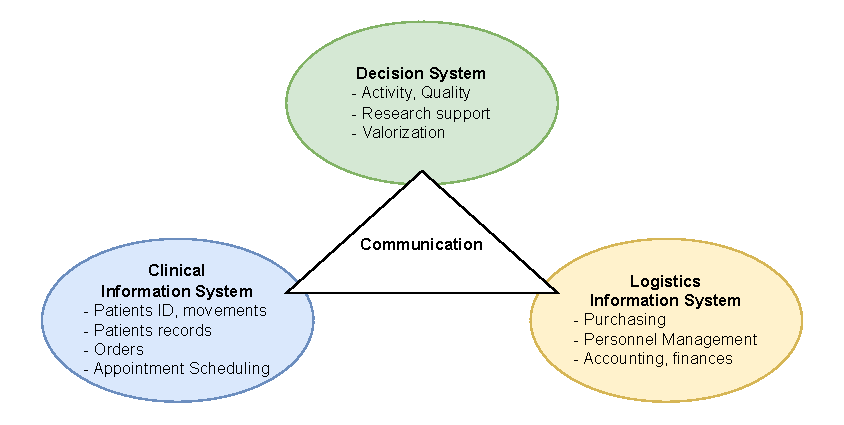
\includegraphics[width=0.9\textwidth]{figures/HIS Schema.pdf} 
    \caption{Functional subsystems in a Hospital Information System, adapted from~\cite{Degoulet_2014}.}
    \label{fig:his-functional}
\end{figure}

The design of a \ac{HIS} is generally component-based~\cite{Van_De_Velde_Degoulet_2003, Winter_Ammenwerth_Haux_Marschollek_Steiner_Jahn_2023}.
%
The components of a \ac{HIS} follow a functional decomposition~\cite{Winter_Ammenwerth_Haux_Marschollek_Steiner_Jahn_2023} separating the core functionalities across different processes. 
%
Classical components of a \ac{HIS} include~\cite{Winter_Ammenwerth_Haux_Marschollek_Steiner_Jahn_2023}:
\begin{itemize}
    \item Patient Administration Systems including \textbf{Patient Identification}, \textbf{Appointment Scheduling (AS)}, \textbf{Admission, Discharge and Transfer (ADT)} and \textbf{Billing and Accounting};
    \item Medical Documentation Systems such as the \textbf{\acp{EHR}} to manage patient medical records, including clinical notes, diagnoses, medications, and allergies, now often integrated to provide a full view of patient data through \textbf{Clinical Data Repositories (CDR)};
    \item \textbf{Operation Management Systems} to support logistics such as planning, bed management and staff schedules for surgeries.
    \item \textbf{Computerized Physician Order Entry (CPOE)} to manage orders for medications, lab tests, imaging, and other procedures;
    \item \textbf{Clinical Decision Support Systems (CDSS)} to provide clinicians with evidence-based recommendations and alerts to support clinical decisions;
    \item ancillary departmental systems such as \textbf{Laboratory Information Systems (LIS)} to manage laboratory tests and results, \textbf{Radiology Information Systems (RIS)} and \textbf{Picture Archiving and Communication Systems (PACS)} to manage imaging studies and results, and \textbf{Pharmacy Information Systems (PIS)} to manage medication orders and dispensing;
    \item \textbf{Document Archiving Systems} to store and manage medical documents for archival and legal purposes. 
\end{itemize}

These core modules are often building the backbone of a \ac{HIS} which can then be correlated with a variety of specific additional systems to support specific needs of the organization. 
%
These include telemedicine systems, patient portals, mobile health applications, and systems for managing specific clinical areas such as oncology or cardiology~\cite{Winter_Ammenwerth_Haux_Marschollek_Steiner_Jahn_2023}.

The level of digitalization and integration of these functional components can significantly impact operations in a healthcare organization. 
%
Maturity assessments of \ac{HIS} are hence crucial to identify gaps and areas of improvement.
%
Several maturity models have been proposed~\cite{Gomes_Romão_2018}, assessing the maturity of \ac{HIS} across various dimensions such as technology, processes, and organizational culture.

A notable example is the \emph{Electronic Medical Record Adoption Model (EMRAM)} by HIMSS~\cite{HIMSS_EMRAM_Criteria}, which assesses the adoption and utilization of electronic medical records in healthcare organizations across eight stages, from 0 (no electronic records) to 7 (fully electronic and integrated systems).
%
The different levels offer a roadmap for healthcare organization to plan their digital transformation journey. 
%
Interestingly, the first levels (following also an historical perspective) focus on the digitalization of ancillary systems first, and follow with the integration of \ac{EHR} in clinical data repositories, highlighting the importance of data integration as a key step in the digital transformation of healthcare organizations.

Other models such as the one proposed in \cite{Carvalho_Rocha_van_de_Wetering_Abreu_2019} also identify different levels, characterizing the maturity of \ac{HIS} in terms of interoperability, data analysis, strategic planning, involved people, availability of electronic medical records, security and technological infrastructure. 
%
The goal of the last levels is to achieve a fully national integrated \ac{HIS} that utilizes real-time data, supports personalized medicine, flexible planning and clinical decision-making, in line with the goals of Healthcare 4.0.

%=======================================================
\section{Medical Standards for Interoperability}
%=======================================================

The complexity of \acp{HIS} and the need for integration across different systems make interoperability a key requirement. 
%
This motivates the need for standards to ensure that different systems can communicate and exchange data effectively. 
%
The complexity of medical data and the variability in medical processes makes the encoding of medical knowledge in such standards a challenging task. 

Over the years, several independent organizations have developed standards to address different aspects of healthcare interoperability~\cite{benson2016principles}.
%
Medical interoperability standards can be broadly categorized into different types based on their purpose and scope: 
\begin{itemize}
    \item \textbf{Terminologies and Coding Systems} provide a common vocabulary for representing medical concepts, diagnoses, procedures and medications. Examples include \ac{ICD} (established by the World Health Organization) for disease classification, \ac{SNOMED-CT} for clinical terminology, and \ac{LOINC} for laboratory and clinical observations.
    \item \textbf{Data Exchange and Transport} standards define how data is exchanged between systems. One of the main example is \ac{HL7} Clinical data Architecture and its new version \ac{FHIR}, which defines a structured information model for exchange of medical data across systems.
    \item \textbf{Specialized Document Formats} are used to represent specific types of medical documents. An example is the \ac{DICOM} standard for medical imaging.
\end{itemize}

These standards are often used in combination to achieve technical and semantic interoperability. 
%
In particular, \ac{FHIR} is the most modern proposal for data exchange in healthcare systems, adopting a modular approach based on the definition of \emph{resources} that can be combined to represent complex clinical concepts, which can be associated with other standard terminologies~\cite{Braunstein_2018}
%
\ac{FHIR} adopts a \ac{REST}~\cite{fielding2000architectural} approach to its \ac{API}, making it easier to integrate with modern Web technologies, breaking out of the traditional silos of healthcare systems. 
%
Despite this choice, \ac{FHIR} is not limited to work in a request-response fashion, but can be integrated as a transport protocol for other communication paradigms such as publish-subscribe or event-based architectures, or even simply to serialize documents for archival purposes~\cite{benson2016principles}.
%
\ac{FHIR} resources can link to other resources, enabling the representation of relationships between entities (e.g., patients, practitioners, medications, observations). 
%
This approach favors the integration of data from multiple sources in a \ac{HIS}, and the pervasive use of \ac{FHIR} as a the format to represent and exchange data in a structured format~\cite{benson2016principles}.

\todo{an image for FHIR?}

\ac{FHIR} resources have a hierarchical structure, with each resource having a defined set of attributes and relationships to other resources.
%
The semantic interpretation of \ac{FHIR} resources is supported by a fixed set of data types, and the support for referencing external terminologies and coding systems, providing unambiguous meaning to the data being exchanged.
%
Furthermore, \ac{FHIR} provides a mechanism for defining profiles and extensions, allowing customization of resources to meet specific use cases while maintaining interoperability with the core standard. 

Due to its versatility and modern design, \ac{FHIR} is increasingly being adopted in healthcare systems~\cite{Ayaz_Pasha_Alzahrani_Budiarto_Stiawan_2021} and also in healthcare research~\cite{Vorisek_Lehne_Klopfenstein_Mayer_Bartschke_Haese_Thun_2022}, making it a key standard for healthcare interoperability today.

A different approach to \ac{EHR} interoperability is taken by the openEHR standards~\cite{openEHR_architecture_overview}, which focus on the multi-level definition of stable \emph{reference models} and domain-specific \emph{archetypes} to represent clinical concepts in a structured and reusable way.
%
The main focus of openEHR is on the modeling of clinical data, rather than on the exchange of data between systems.
%
This makes openEHR more suitable for the design of clinical data repositories and \ac{EHR} systems~\cite{Delussu_Frexia_Mascia_Sulis_Meloni_Del_Rio_Lianas_2024}.
%
The standard further provides guidelines on management of \ac{EHR} including versioning, auditing and access control which are crucial for the management of sensitive medical data. 
%
OpenEHR can hence be considered complementary to other standards, focusing on the management and storage of \ac{EHR} data~\cite{Bosca_Moner_Maldonado_Robles_2015,Pedrera-Jiménez_García-Barrio_Frid_Moner_Boscá-Tomás_Lozano-Rubí_Kalra_Beale_Muñoz-Carrero_Serrano-Balazote_2023}. 

This section provides a brief overview of the main standards for healthcare interoperability. 
%
The abundance of standards clearly reflects the complexity of the healthcare domain both in terms of the intrinsic complexity of medical data and processes and the variety of stakeholders and organizations involved.
%
Adopting and combining effectively these standards is a key requirement for the design of modern \acp{HIS} towards the implementation of Healthcare 4.0 objectives.
%
Semantic interoperability is still an open challenge as the standards partially overlap and are not supported by formal ontological models which could remove ambiguities and improve deductive reasoning~\cite{de_Mello_Rigo_da_Costa_da_Rosa_Righi_Donida_Bez_Schunke_2022}.
%
In this sense, alignment with Semantic Web technologies~\cite{berners2023semantic} and ontologies could provide a pathway towards achieving greater semantic interoperability in healthcare~\cite{Schulz_Martínez-Costa_2013}.

%=======================================================
\section{Intelligent Applications in Healthcare}
%=======================================================

\todo{maybe find an image for AI applications..}

Among the drivers of Healthcare 4.0, \ac{AI} is playing an increasingly important role in healthcare.
%
Due to its inherent complexity, healthcare has always been a target domain for \ac{AI} applications, as the possibility to ease the burden of healthcare professionals and improve the quality of care is a strong motivation for innovation. 
%
While originally most \ac{AI} applications in healthcare focused on rule-based symbolic reasoning and expert decision-support systems to support clinical decisions, the recent advantages in \ac{ML} and \ac{DL} and the availability of large amounts of data have made data-driven approaches more feasible~\cite{Yu_Beam_Kohane_2018}.
%
Recent surveys confirm that the rate of scientific publications on \ac{AI} in healthcare is growing at a very fast pace covering a wide range of applications~\cite{Secinaro_Calandra_Secinaro_Muthurangu_Biancone_2021,Yousefi_Dehnavieh_Laberge_Gagnon_Ghaemi_Nadali_Azizi_2025}.

Applications of \ac{AI} techniques in healthcare span across a wide range of areas.
%
One of the most significant is image-based diagnosis, where \acp{CNN} for image classification have shown performances comparable or even superior to human experts in recognizing pathologies from medical images.
%
Other relevant applications include genome interpretation, biomarker discovery, risk estimation and prediction of clinical outcomes, and continuous monitoring through \ac{IoT} stream analysis~\cite{Yu_Beam_Kohane_2018}.

More recently, the advent of \acp{LLM} and \ac{GenAI} technologies is opening new possibilities for \ac{AI} applications in healthcare~\cite{Sai_Gaur_Sai_Chamola_Guizani_Rodrigues_2024}.
%
\ac{GenAI} techniques can be used for data augmentation, to generate synthetic medical data and support training of \ac{ML} models when real data is scarce. 
%
\acp{LLM} can be used to analyze and produce medical documents and their adoption is growing at a fast pace especially for the automatic draft of clinical documentation from conversations with the overall objective of increasing efficiency by automating repetitive tasks~\cite{Poon_Lemak_Rojas_Guptill_Classen_2025}.
%
Additionally, \ac{LLM} can be used to interact with patients through chatbots, providing information and support for common medical questions and concerns.
%
Fine-tuned medical \acp{LLM} can also be used to support clinical decision-making and summarization of medical literature~\cite{Sai_Gaur_Sai_Chamola_Guizani_Rodrigues_2024}.

Secinaro et al.~\cite{Secinaro_Calandra_Secinaro_Muthurangu_Biancone_2021} identify three main clusters of application of \ac{AI} in healthcare:
\begin{itemize}
    \item predictive models for diagnosis and monitoring of patients
    \item decision support systems to support decision-making
    \item big data analytics to optimize healthcare operations and management
\end{itemize}

This multi-faceted approach highlights the wide scope of \ac{AI} applications in healthcare which can target both clinical and administrative processes.

Given the critical nature of healthcare, the adoption of \ac{AI} requires careful consideration of ethical implications~\cite{Morley_Machado_Burr_Cowls_Joshi_Taddeo_Floridi_2020}.
%
In general \ac{AI} systems are seen as tools to improve human decision-making, making it possibly more objective and data driven.
%
Of course this requires carefully designed systems and data collection processes to avoid introducing new sources of errors and biases which may undermine the benefits~\cite{Norori_Hu_Aellen_Faraci_Tzovara_2021}.

The reliance on \ac{AI} systems for clinical decisions can also raise concerns of misdiagnosis due to the possibility of overestimating the confidence of automated systems~\cite{Morley_Machado_Burr_Cowls_Joshi_Taddeo_Floridi_2020}.
%
New trends are hence focusing on explainability and interpretability of \ac{AI} systems which becomes a crucial property for the deployment of \ac{AI} systems in healthcare~\cite{Bharati_Mondal_Podder_2024}.
%
\ac{XAI} techniques are being increasingly required in healthcare~\cite{Freyer_Groß_Lipprandt_2024} settings due to the need for transparency in the decision-making process which is crucial for building trust: a necessary condition for the successful acceptance of \ac{AI} by both patients and healthcare professionals~\cite{Alonso_Astobiza_Ortega_Lozano_2025}.

Finally, regulations play a crucial role in the effort to ensure that \ac{AI} systems in healthcare are safe and ethical~\cite{Freyer_Groß_Lipprandt_2024}.
%
These need to be accompanied by guidelines and best practices that promote careful design and implementation of \ac{AI} models, from data collection, selection and preprocessing, to model training and validation~\cite{de_Hond_Leeuwenberg_Hooft_Kant_Nijman_van_Os_Aardoom_Debray_Schuit_van_Smeden_et_al._2022}.


%=======================================================
\section{The \ausl{} Context}
%=======================================================

\auslLong{} is the local public healthcare administration for the Emilia-Romagna region in Italy, covering a population of more than 1.1 million people across a territory of roughly 5100 km$^2$ which covers the provinces of Ravenna, Forlì-Cesena and Rimini and is divided into 8 health districts (\Cref{fig:ausl-map}).
%
The organization manages 7 main hospitals hubs comprising a total of 13 hospital facilities and several other care centers managed by a network of more than 16 thousands employees. 
%
Born from the merger of three different local healthcare administrations in 2013, \ausl{} is among the largest healthcare providers in Italy.
%
The high complexity of the organization and the large territory it covers make \ausl{} a relevant case study for the challenges of digital transformation in healthcare as, due to its historical evolution it deals with integration of heterogeneous systems and processes across different settings and can represent a microcosm of the challenges faced by the healthcare sector in general.


\begin{figure}[t]
    \centering
    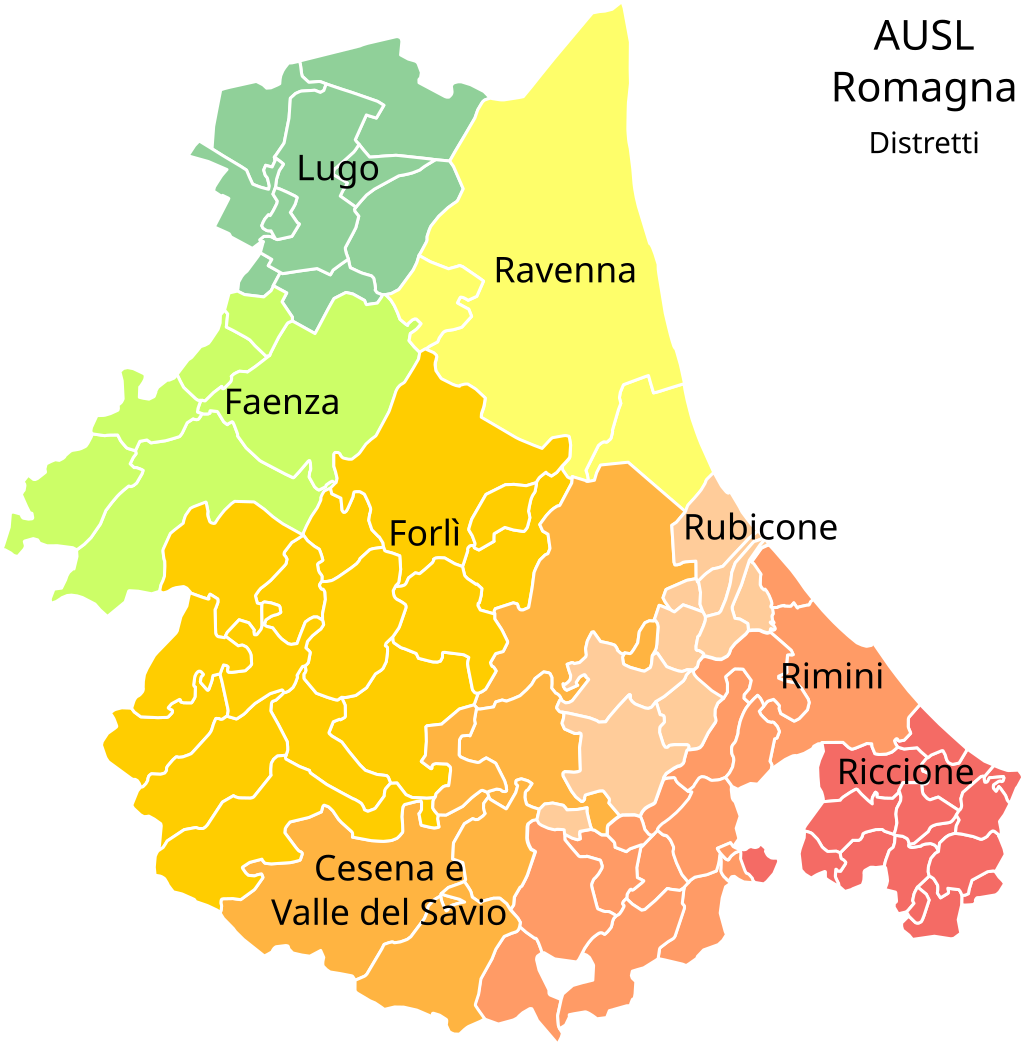
\includegraphics[width=0.55\textwidth]{figures/mappa_ausl.png} 
    \caption{
        Map of the \ausl{} territory, credits:
        \url{https://commons.wikimedia.org/wiki/File:Mappa_dell\%27AUSL_Romagna.svg}
    }
    \label{fig:ausl-map}
\end{figure}


\ausl{}, aligned with the objectives of the national healthcare plans, is pursuing a digital transformation process aimed at improving the efficiency and effectiveness of its services.
%
A first essential step in this direction has been the adoption of a personal \ac{EHR} system directly accessible by patients (\emph{Fascicolo Sanitario Elettronico (FSE)}).
This system allows patients to access their health records, book appointments, and communicate with healthcare providers more easily. 
%
Emilia-Romagna has been the Italian region with the highest success rate in the implementation of FSE~\cite{fse_ausl_prima} with over 65\% of the population having accessed their FSE at least once and more than 90\% of the population agreeing to its consultation by healthcare professionals.

The digitalization program has been accelerated by the COVID-19 pandemic, which has highlighted the need for more agile and resilient healthcare systems worldwide.
%
The NextGenerationEU programme of the European Union funds several initiatives in its member states as a response to the COVID-19 pandemic. 
%
In Italy, this has been translated into the \emph{Piano Nazionale di Ripresa e Resilienza (PNRR)} which includes several \emph{missions}.
Mission 1 includes as a key objective the which digitalization of public administrations, including healthcare organizations. 
Mission 6 is instead entirely dedicated to the innovation of healthcare services, targeting the technological improvement of hospitals, decentralization of healthcare services, telemedicine and remote care~\cite{italy_pnrr_2021}.
%
This PhD work is also funded under PNRR, under Mission 4 promoting the collaboration of industrial partners and research institutions.

\ausl{} is continuing its digital transformation journey within this framework.
%
A strategic plan for its digitalization (``Progetto Sanità Digitale'') has been defined in 2021 to guide the process as a collaboration between \ausl{}, the Computer Science and Engineering Department of the University of Bologna and the oncologic care and research center {Istituto Romagnolo per lo Studio dei Tumori ``Dino Amadori''(IRST)}, members of a local lavoratory for healthcare innovation (Laboratiorio Sanità Digitale~\footnote{\url{https://laboratorio-sanita-digitale.github.io/}})~\cite{progetto_sanità_digitale}.
%
Key objectives of the digitalization plan include the decentralization and distribution of care with local care centers and remote monitoring, the integration of data from multiple sources to support personalized medicine and the improvement of operational efficiency. 
%
A strategic technology envisioned in this context is the adoption of \emph{\acp{DT}~\cite{Grieves_2023}}, which can offer an aggregation point for data and functionalities from multiple systems tailored to the representation of critical assets in the healthcare organization~\cite{progetto_sanità_digitale}.

This thesis work is framed within this context, exploring the role of \acp{DT} as enablers of Healthcare 4.0 objectives and focusing on the challenges of interoperability and data integration in a complex and distributed healthcare organization such as \ausl{}.

%=======================================================
\section{Final Remarks}
%=======================================================

This chapter provides an overview of the context of Healthcare 4.0 which motivates and frames the work presented in this thesis. 
%
The digital transformation of healthcare is a complex process that involve multiple dimensions, from technological to organizational and socio-economic factors.

The chapter highlights the multi-faceted nature of the healthcare domain, and the efforts that are being pursued towards improving digitalization, with a focus on \ac{HIS} as the exemplary case of \ac{ICT} systems in healthcare which motivates the need for interoperability and data integration.

The chapter further reflects on the role of \ac{AI} in healthcare, showing how it can address both clinical and organizational challenges, emphasizing the critical requirements the domain imposes on the design of intelligent applications that are trustworthy, reliable and fair.

Finally, the chapter describes the context of \ausl{} as the partner organization for this thesis work, highlighting the relevance of the challenges faced by the organization in its digital transformation journey which motivate this thesis work. 

%%%%%%%%%%%%%%%%%%%%%%%%%%%%%%%%%%%%%%%%%%%%%%%%%%%%%%%%
\chapter{\aclp{DT}}
\label{chap:back:DT}
%%%%%%%%%%%%%%%%%%%%%%%%%%%%%%%%%%%%%%%%%%%%%%%%%%%%%%%%

This chapter provides an overview of the \ac{DT} concept,
its historical development and the more recent models and technologies that have emerged
to support its implementation.
%
The ever-growing literature on the subject reflects the increasing interest in \acp{DT}
and its multi-faceted nature, encompassing various domains and applications.
%
In this thesis we focus on the software engineering perspective of \acp{DT}, 
and the application of \acp{DT} to the engineering of \ac{IoT} systems.
%
Accordingly, this chapter focuses on how the \ac{DT} concept has been interpreted in this context.


%=======================================================
\section{History and Definitions}
%=======================================================

The concept of \ac{DT} was introduced in the early 2000s by Michael Grieves
in the context of Product-Lifecycle Management~\cite{Grieves_2023}
where it was conceived as a virtual representation of a product throughout its lifecycle.
%
At its essence, Grieves defined what later came to be known as a \ac{DT} as a system composed of three main components (\Cref{fig:dt-grieves-original}):
\begin{itemize}
\item a \emph{physical space} and its products;
\item a \emph{virtual space} containing the digital representation of the products;
\item a \emph{connection} between the two, making data flow from the physical to the virtual space and information flow from the virtual to the physical space~\cite{Grieves2017}.
\end{itemize}

\begin{figure}[t]
    \centering
    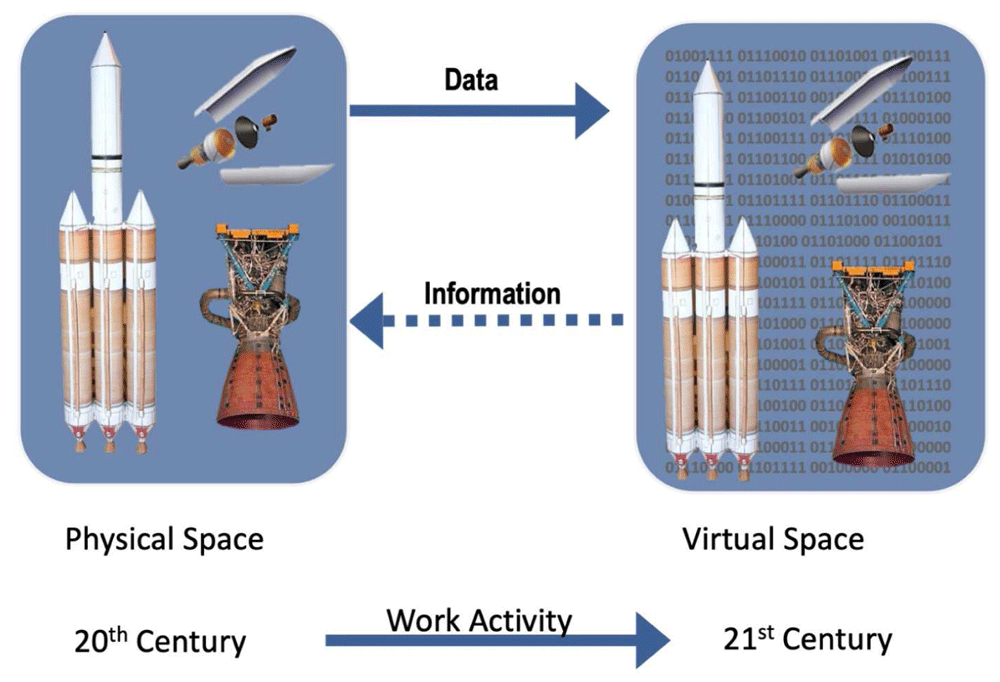
\includegraphics[width=0.7\textwidth]{figures/dt-original.png}
    \caption{The original \ac{DT} model by Grieves, from \cite{Grieves_2022}.}
    \label{fig:dt-grieves-original}
\end{figure}

Grieves referred to this concept as the \emph{Mirrored Spaces Model}~\cite{Grieves_2005},
a name which echoes the idea of \emph{Mirror Worlds} introduced by David Gelernter in the 1990s~\cite{gelernter1991mirrorworlds}
who also envisioned the ability to replicate the real world in a completely virtual space~\cite{Singh_Fuenmayor_Hinchy_Qiao_Murray_Devine_2021}.

The idea was later associated with its modern \emph{\acl{DT}} name and popularized by NASA in the 2010s, when it was presented as a key technology
for future development of aircraft and spacecraft in order to virtually simulate extreme conditions,
integrate data from the physical system in operation, 
and provide feedback on the conditions of the \emph{flying twin}
while possibly enacting changes to mitigate damage~\cite{glaessgen2012dtnasa}.
%
NASA's definition hence focused on the ability of the \ac{DT} to integrate multiple simulation models and characterized the \ac{DT} as \emph{ultra-realistic}, as the goal was to virtually replicate the physical system with the highest possible degree of fidelity:

\begin{quote}
    A Digital Twin is an integrated multiphysics, multiscale, probabilistic simulation of an as-built vehicle or system that uses the best available physical models, sensor updates, fleet history, etc., to mirror the life of its corresponding flying twin~\cite{glaessgen2012dtnasa}.
\end{quote}

Given the various phases of a product's lifecycle, the \ac{DT} concept was later
refined to distinguish between the \emph{Digital Twin Prototype} (DTP) and the \emph{Digital Twin Instance} (DTI) and \emph{Digital Twin Aggregate} (DTA)~\cite{Grieves2017}.
The DTP is the virtual representation of the product during its design and development phase,
while the DTI is the virtual representation of the product during its operational phase.
%
The DTA represents instead the aggregation of all DTIs, hence all products that have been built~\cite{Grieves_2022}.
%
Interestingly, the DTP exists before the physical product is even produced, 
and it is rather ``just'' a virtual model of the product. 
%
Grieves argues that requiring that a \ac{DT} exists only when the physical product exists is a \emph{fallacy}~\cite{Grieves_2022}.
%
Nevertheless, it is generally accepted within the community nowadays that, for a proper characterization, what is usually referred as \ac{DT} is hence a DTI, which exists alongside its physical counterpart and is continuously updated with data from the physical world. 

The role of such bidirectional data exchange between the physical and virtual parts
of a \ac{DT} has been, in fact, used to characterize the \ac{DT} concept and distinguish it from other related concepts.
%
A widely accepted taxonomy classifies the concepts of \emph{Digital Model}, \emph{Digital Shadow} and \emph{Digital Twin} based on direction of the automatic data flow between the physical and virtual spaces~\cite{kritzinger2018dtmanufacturing} (\Cref{fig:dt-taxonomy}):
namely, 
a Digital Model (\Cref{fig:dt-taxonomy-digital-model}) is a static model of a physical system (similarly to the DTP) that can be manually updated over time,
the Digital Shadow (\Cref{fig:dt-taxonomy-digital-shadow}) gets automatically updated through an inbound data flow from the physical space,
while the Digital Twin (\Cref{fig:dt-taxonomy-digital-twin}) is the only one that holds a bidirectional data flow which can provide feedback to the physical counterpart.
%
Such connection has been referred to as the \emph{digital thread}~\cite{Singh_Willcox_2018,Grieves_2023} to evoke the idea of a tie that binds the physical and virtual spaces.
%
Other common terms include \emph{twinning}~\cite{JONES202036} or \emph{shadowing}~\cite{Jiang_Yin_Li_Luo_Kaynak_2021,web-of-dt-ricci-2022} process. 
%
This terminology emphasizes the continuous and dynamic nature of the relationship between the physical and virtual entities, 
and highlights the active role of such process in maintaining the \ac{DT} up to date.

\begin{figure}[t]
    \centering
    \begin{subfigure}[b]{0.3\linewidth}
        \centering
        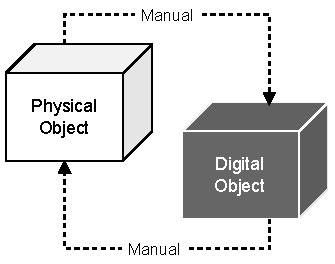
\includegraphics[width=\linewidth]{figures/kritzinger-digital-model.pdf}
        \caption{Digital Model}
        \label{fig:dt-taxonomy-digital-model}
    \end{subfigure}
    \hfill
    \begin{subfigure}[b]{0.3\linewidth}
        \centering
        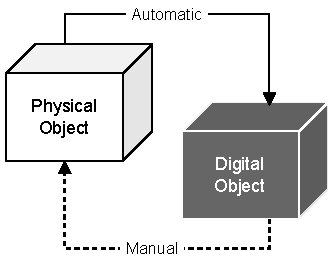
\includegraphics[width=\linewidth]{figures/kritzinger-digital-shadow.pdf}
        \caption{Digital Shadow}
        \label{fig:dt-taxonomy-digital-shadow}
    \end{subfigure}
    \hfill
    \begin{subfigure}[b]{0.3\linewidth}
        \centering
        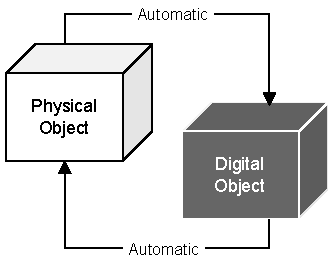
\includegraphics[width=\linewidth]{figures/kritzinger-digital-twin.pdf}
        \caption{Digital Twin}
        \label{fig:dt-taxonomy-digital-twin}
    \end{subfigure}
    \caption{Taxonomy of Digital Twin related concepts based on the data flows between physical and digital objects, adapted from \cite{kritzinger2018dtmanufacturing}.}
    \label{fig:dt-taxonomy}v
\end{figure}

The scope and applicability of the \ac{DT} concept has evolved and expanded
to encompass a wide range of applications and domains.
%
Today, \acp{DT} are used in various fields such as manufacturing, healthcare, smart cities, and more.
%
This is also reflected in the abundance of terminology used to identify the physical counterpart of a \ac{DT}
which is nowadays often referred to as the \emph{physical twin} or
\emph{physical entity}~\cite{Singh_Fuenmayor_Hinchy_Qiao_Murray_Devine_2021,JONES202036,DBLP:journals/jss/DaliborJRSWWW22}.
%
This shift from identifying the physical counterpart as a \emph{product} to a more generic \emph{entity}
highlights the broader applicability of the \ac{DT} concept beyond its original manufacturing context.
%
The \ac{DT} concept has been adopted also to represent people~\cite{Shengli_2021},
processes (e.g., supply chain~\cite{Barykin_Bochkarev_Kalinina_Yadykin_2020}) and organizations~\cite{Parmar_Leiponen_Thomas_2020}, leading to a more abstract interpretation of what can be considered \emph{physical}. 
%
Accordingly, the definitions of \acp{DT} have also diversified, leading to a plethora of interpretations~\cite{DBLP:journals/jss/DaliborJRSWWW22}. 

For the scope of this thesis, 
since the focus is on how \acp{DT} can be used to engineer \ac{IoT} systems, taking as the reference context the healthcare domain,
we adopt the following definition, adapted from \cite{dt-IoT-context-Minerva-2020}:

\begin{quote}
A \acf{DT} is a comprehensive software representation of an individual \acl{PA}.
It includes the properties, conditions, and behavior(s) of the real-life asset through models and data.
A \ac{DT} is a set of realistic models that can simulate an asset's behavior in the deployed environment.
The \ac{DT} represents and reflects its physical twin and remains its virtual counterpart across the asset's entire lifecycle.
\end{quote}

The definition emphasizes the software nature of the \ac{DT} and its ability to model the properties and behavior of its physical counterpart.
%
We deliberately use the term \emph{\ac{PA}} to refer to the physical counterpart of a \ac{DT}
to highlight the fact that an \emph{asset} is something that has a strategic
value in the context of an application domain, and that the \ac{DT} is meant to represent and manage such assets.
%
Compared to the original Grieves model which characterized the \ac{DT} as having three parts (physical, digital and connection), for the reminder of this thesis we will instead consider:
\begin{itemize}
\item the \ac{PA} as the physical counterpart of a \ac{DT};
\item the \ac{DT} as the software implementing the virtual representation of the \ac{PA} through a combination of models and data;
\item the \emph{twinning process} implemented by the \ac{DT} software to keep the \ac{DT} up to date with the \ac{PA} and possibly provide feedback to it.
\end{itemize}

%=======================================================
\section{Reference Architectures and Properties}
%=======================================================

The conceptual definition of \ac{DT} gives little indication on how to implement it,
leaving a degree of freedom in the technical realization of the \ac{DT} software.
%
For this reason, a variety of reference architectures have been proposed, 
each emphasizing different aspects of the \ac{DT} concept~\cite{ferko2022architecting}.

One that has gained significant recognition in the \ac{DT} community is the \emph{five-dimensional model} (5D model) by Tao et al.~\cite{dt-driven-prognostics-tao-2018}.
%
As shown in \Cref{fig:dt-5d-model}, the 5D model characterizes a \ac{DT} as composed of five main components~\cite{qi2021enablingtechdt}:
\begin{itemize}
\item the \emph{physical entity} (PE), which is the physical counterpart of the \ac{DT};
\item the \emph{virtual models} (VM), which is the digital representation of the PE possibly including 3D models, rules and behavioral models;
\item the \emph{data} (DD), which includes all data related to the PE and possibly generated by the VM, such as historical data, real-time data, simulation results;
\item the \emph{service} (Ss), which encompasses all services provided by the \ac{DT} to users, such as monitoring, simulation, diagnostics, and optimization;
\item the \emph{connection} (CN), which represents the communication and data exchange between all other components, there including the bidirectional connection between the PE and the VM that is fundamental for the \ac{DT} operation.
\end{itemize}

\begin{figure}[t]
    \centering
    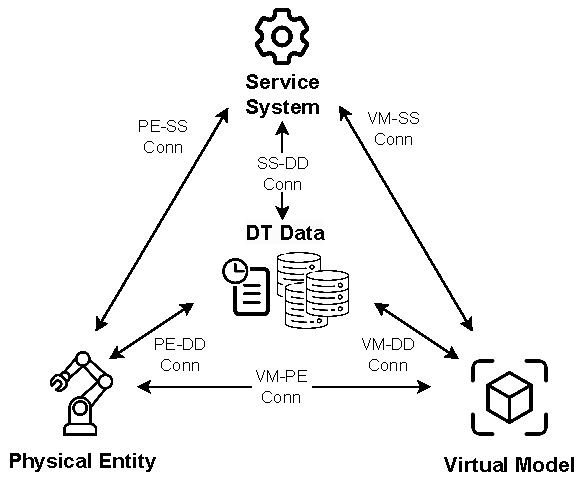
\includegraphics[width=0.6\textwidth]{figures/5d-model.pdf}
    \caption{The 5D model of a Digital Twin.}
    \label{fig:dt-5d-model}
\end{figure}

Tao's 5D model extends Grieves' original model by explicitly including the data and services dimensions, better characterizing the \ac{DT} as a data-driven and service-oriented system. 


The service-oriented nature of \acp{DT} has an essential role in their ability to provide value to users.
%
The \ac{DT} is hence not just a passive representation of a \ac{PA}, but an active system that users can interact with to obtain insights and perform actions on the \ac{PA}.
%
This also contrasts the idea of the \ac{PA}-\ac{DT} system as a closed-loop control system, but rather envisions the \ac{DT} as open to interactions with external entities such as human users or other software systems.

Following this perspective, the idea of \ac{DT}-as-a-service has been proposed.
As shown in \Cref{fig:dt-as-a-service}, the proposed reference architecture adds a cyber layer and an application layer on top of the classic physical, digital and communication layers of a \ac{DT}~\cite{aheleroff2021aei}.
%
The reference architecture further highlights different levels of integration following the taxonomy of Digital Model, Shadow, and Twin~\cite{kritzinger2018dtmanufacturing}, with a further Digital Twin predictive level, which includes predictive models and analytics capabilities enabled by the cyber layer grounded on cloud technologies such as Big Data analytics. 
%
The vision additionally integrates \acp{DT} in an incremental and iterative development lifecycle, to accompany and evolve alongside the \acp{PA} they represent. 

\begin{figure}[t]
    \centering
    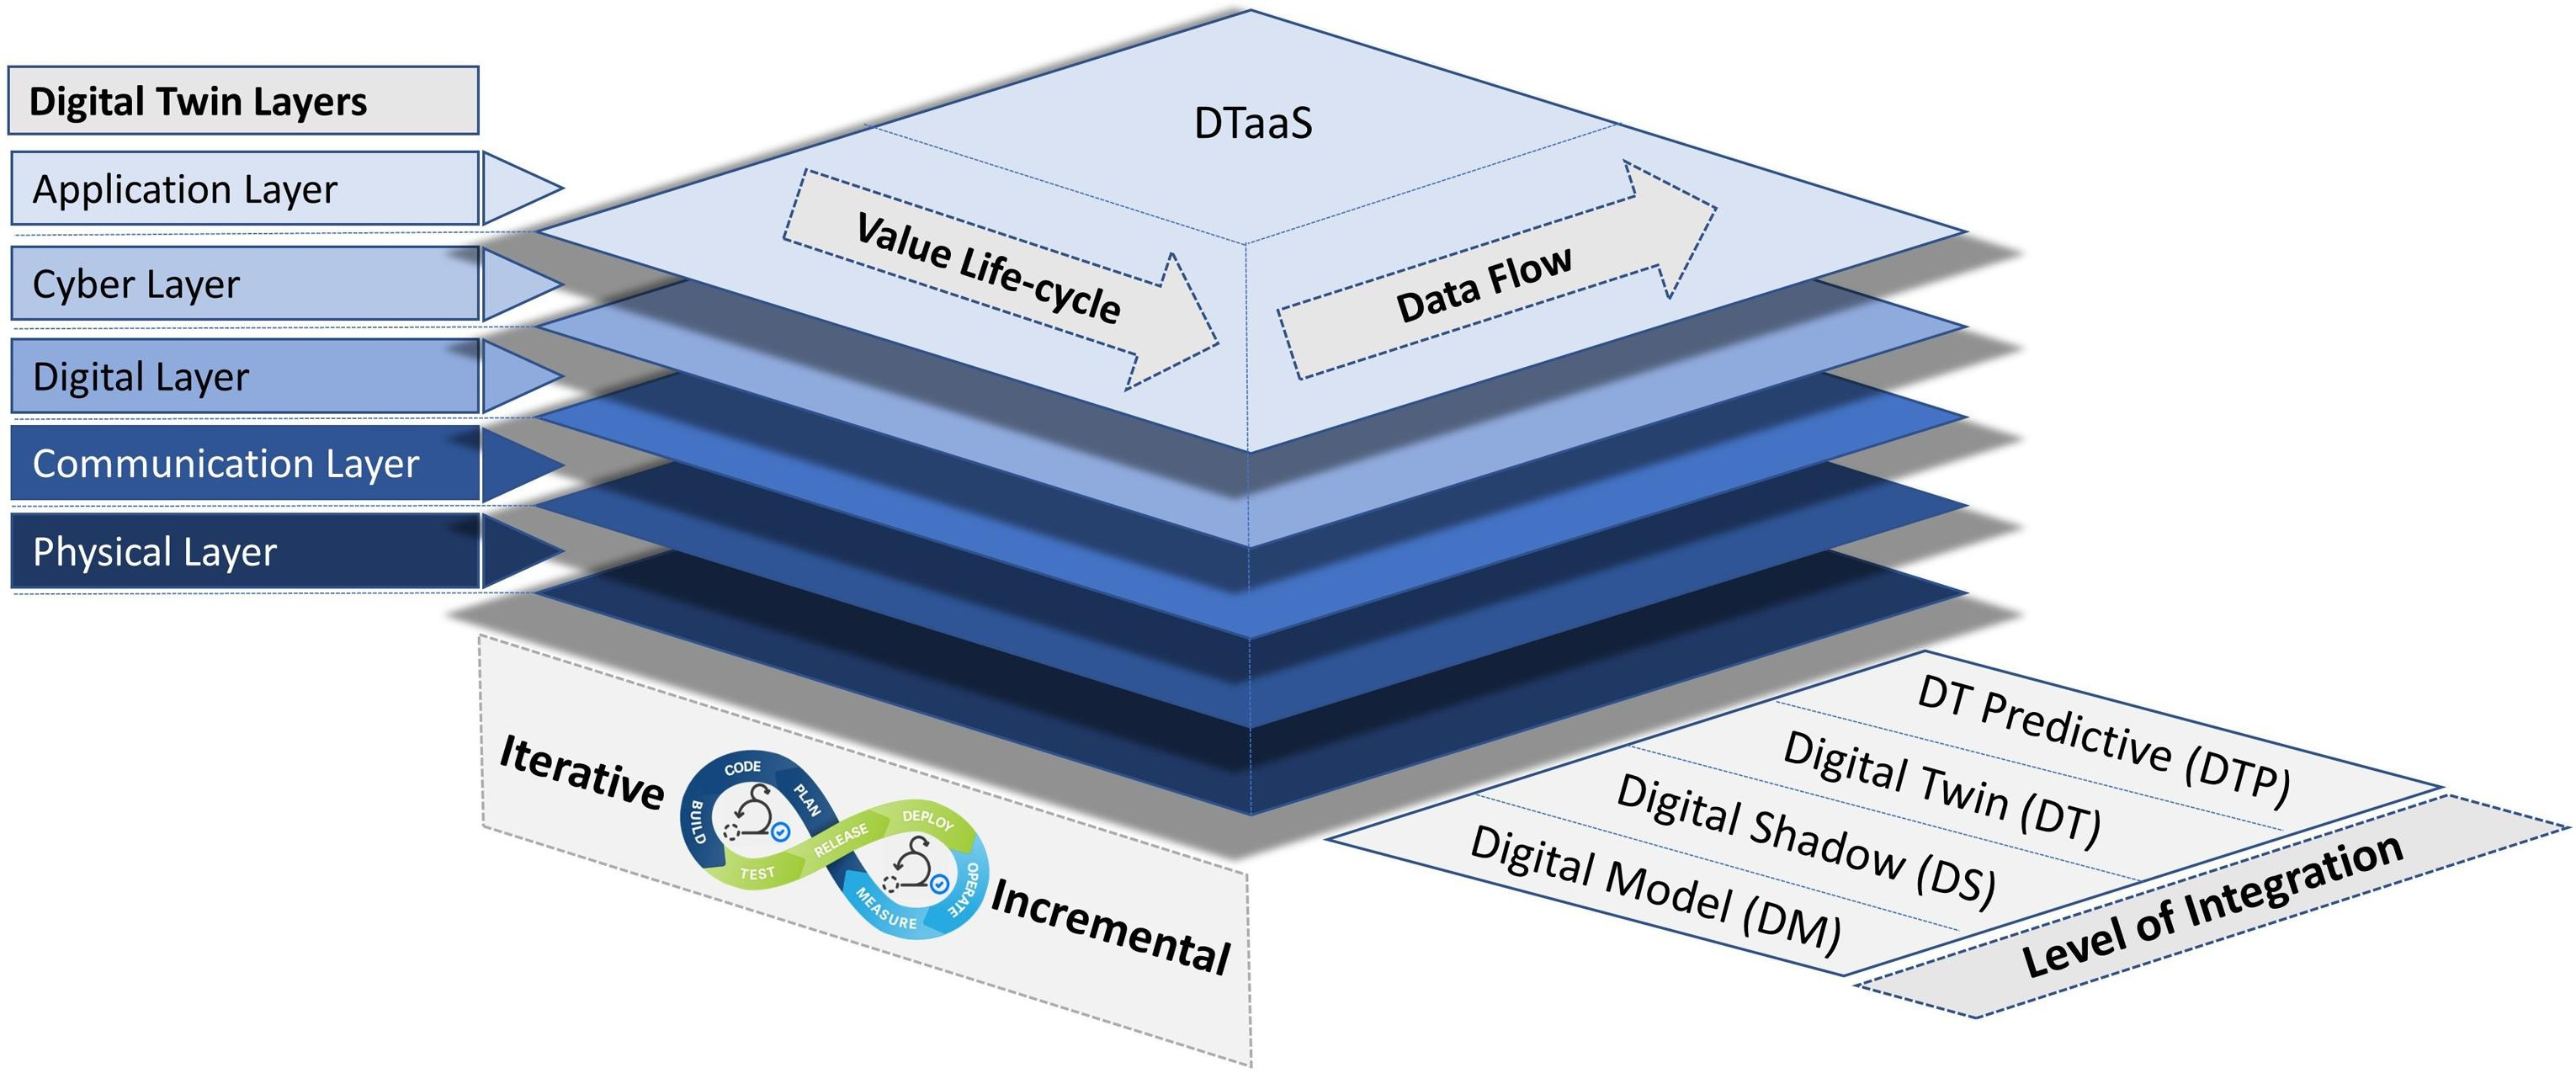
\includegraphics[width=\textwidth]{figures/dt-as-a-service.jpg}
    \caption{The DT-as-a-Service reference architecture, from \cite{aheleroff2021aei}.}
    \label{fig:dt-as-a-service}
\end{figure}

Layered and service-oriented architectures for \acp{DT} are the most popular in the literature.
%
These architectures support desired non-functional quality attributes such as performance efficiency, reliability and maintainability, but also compatibility with existing systems and scalability~\cite{ferko2022architecting}

On the functional side, \cite{dt-IoT-context-Minerva-2020} proposes a set of properties \ac{DT} should have, analyzing existing literature and implementations in the \ac{IoT} context.
%
The properties, summarized in \Cref{tab:minerva-properties} detail various aspects that characterize functional behavior of \acp{DT}.
%
Interestingly, such properties go beyond the generic definition of \ac{DT} as a virtual representation of a \ac{PA} and highlights the various capabilities that a \ac{DT} can provide to its users.

First, both the \ac{DT} and the \ac{PA} are required to be \emph{univocally identifiable} in order to establish a clear relationship between the two. This vision supports the possibility of having possibly multiple \acp{DT} representing the same \ac{PA} in different contexts or for different purposes.
%
Accordingly, the second important contribution is the emphasis on \emph{contextualization}. 
This shifts the focus from the ultra-realistic \ac{DT} envisioned by NASA to a more pragmatic approach where the \ac{DT} is representative of the \ac{PA} in a specific context,
hence possibly abstracting away details of the \ac{PA} that are not relevant for the intended use of the \ac{DT} in the target system.
%
Additional properties emphasize the dynamic nature of the \ac{DT} and its ability to reflect changes in the \ac{PA} (\emph{reflection}), in a timely manner (\emph{entanglement}), persisting over time (\emph{persistence}), memorizing past states (\emph{memorization}) and offering a reliable representation of the \ac{PA} (\emph{accountability}). 
%
Finally, the properties also highlight the ability of \acp{DT} to provide value to users through services (\emph{servitization}) such as aggregation of multiple assets (\emph{composability}), augmentation of the \ac{PA} capabilities (\emph{augmentation}), management of access control (\emph{ownership}), and anticipation of future states and behaviors of the \ac{PA} (\emph{predictability}).

\begin{table}[t]
\centering
\caption{Characterizing Properties of \acp{DT}, defined in \cite{dt-IoT-context-Minerva-2020}.}
\renewcommand{\arraystretch}{1.3}
\begin{tabular}{p{3.5cm}|p{\dimexpr\textwidth-4.5cm\relax}}
\toprule
\midrule
\textbf{Property} & \textbf{Description} \\
\midrule
\toprule
{Contextualization} & A \ac{DT} models the \ac{PA} in a way that is representative with regard to the target context. \\
\hline
{Reflection} & A \ac{DT} reflects changes in the \ac{PA} in real-time. \\
\hline
{Replication} & A \ac{DT} replicates an object into different environments. \\
\hline
{Entanglement} & The degree to which a \ac{DT} is interconnected with its \ac{PA}. \\
\hline
{Persistency} & A \ac{DT} persists over time even when the \ac{PA} is not available. \\
\hline
{Memorization} & A \ac{DT} stores and allows retrieving past states and events. \\
\hline
{Composability} & A \ac{DT} can aggregate different assets or \acp{DT}. \\
\hline
{Accountability} & A \ac{DT} recovers from errors and maintains a reliable state.\\
\hline
{Augmentation} & A \ac{DT} can add new capabilities to the \ac{PA}.\\
\hline
{Ownership} & A \ac{DT} manages access control over its data and functionalities.\\
\hline
{Servitization} & A \ac{DT} provides services to its users.\\
\hline
{Predictability} & A \ac{DT} can anticipate future states and behaviors of the \ac{PA}.\\
\midrule
\bottomrule
\end{tabular}%
\label{tab:minerva-properties}
\end{table}



%=======================================================
\section{Enabling Technologies and Platforms}
%=======================================================

On a practical level, the implementation of \acp{DT} has been enabled by the convergence of various technologies.
%
This includes the proliferation of \ac{IoT} devices, 
advancements in Big Data analytics and \ac{AI}, 
and an increased availability of computing power to run simulations, 
which make possible to collect and analyze large amounts of data from the physical world, 
derive models of the \ac{PA} and execute them to obtain insights~\cite{qi2021enablingtechdt,Fuller_Fan_Day_Barlow_2020,Mihai_survey_enabling_2022}.

On the physical side, the availability of network-connected sensors and actuators enable the acquisition of real-time data from the \ac{PA}.
%
Sensing technologies for \ac{DT} broadly include classic \ac{IoT} techniques such as RFID, digital sensors,
but also computer vision and image processing.
%
In many cases, the data that can be automatically collected from the \ac{PA} is complemented by manual data entry, making the \ac{DT} interact with other information systems.
%
Sensing is followed by connectivity and data exchange, through a variety of communication protocols and network technologies.
%
\acp{DT} may need to operate with different data sources, each with its own communication protocol and data format.
%
Classic examples of \ac{IoT} communication protocols include MQTT, CoAP, HTTP, and WebSocket, but also industrial protocols such as OPC-UA and Modbus~\cite{Fortino_Savaglio_2023}. 
%
Finally, the physical layer includes a computing infrastructure that can span from the edge to the cloud, to support the data acquisition, processing and storage needs of the \ac{DT}.

On the virtual side, the \ac{DT} requires modeling techniques to represent its properties and behaviors.
%
Depending on the application domain this can range from geometrical and physical models, to behavioral models such as finite state machines or process models.
%
Models can be manually created by experts, or automatically derived from data through data-driven modeling and machine learning techniques~\cite{Tao_Xiao_Qi_Cheng_Ji_2022}.
%
Models can be used to simulate the behavior of the \ac{PA} with different simulation software.
%
The volume and variety of data that can be collected from the \ac{PA} and from the \ac{DT} models requires Big Data technologies to extract insights~\cite{Tao_Cheng_Qi_Zhang_Zhang_Sui_2018}. 
%
Finally, the \ac{DT} software needs to provide services to its users, including data visualization technologies, user interfaces and \acp{API} to interact with other software systems.
%
Some further include \ac{AR} and \ac{VR} technologies in the enabling technologies of \acp{DT} to provide immersive experiences to users and visualize \ac{DT}~\cite{Mihai_survey_enabling_2022}.

\todo{maybe a table or something to break the text... }

Due to the complexity of the technological stack required to implement \acp{DT}, the industry has seen the emergence of various supporting tools.
%
First examples of \ac{DT} development tools were developed by large industrial companies such as General Electric's Predix, Siemens MindSphere, PTC ThingWorx, and IBM Watson \ac{IoT}~\cite{Fuller_Fan_Day_Barlow_2020,Adamenko_Kunnen_Nagarajah_2020}.
%
Additionally, several simulation tools such as  ANSYS Twin Builder~\cite{ansys_twinbuilder}, SimuLink~\cite{mathworks_digitaltwin} and AnyLogic~\cite{anylogic_digitaltwin} started to include features to support \ac{DT} development. 
%
Many of these tools, emerging from industrial domains, are tailored to specific use cases and application domains.
%
Additionally, being proprietary software, they often lack openness and interoperability becoming closed silos from a broader system engineering perspective. 

More recently, cloud providers have started to offer so-called \emph{\ac{DT} platforms} such as Microsoft's \azureTwin{}\footnote{\url{https://azure.microsoft.com/en-us/services/digital-twin/}} and Amazon's \awsTwin{}\footnote{\url{https://aws.amazon.com/iot-twinmaker/}}.
%
These general-purpose platforms complement the existing cloud-based \ac{IoT} middlewares with specific features to support the implementation of \acp{DT}. 
This includes the ability to model assets with defined data schemas, providing identification and tracking state properties,
as well as tools to integrate data from various sources, and to grant access to the \ac{DT} data and functionalities through well-defined common \acp{API}.
%
Interestingly, these platforms put forth the idea of having multiple \acp{DT} connected together to represent a complex application domain. 
%
As an example, \azureTwin{} is based on the concept of a \emph{digital twin graph} where multiple \acp{DT} can be connected together to represent complex systems~\cite{Meijers_2022}.
%
Additionally, these platforms are not tied to specific application domains, paving the way for a broader adoption of the \ac{DT} concept. 

Last, but not least, open-source \ac{DT} platforms are emerging~\cite{Gil_Mikkelsen_Gomes_Larsen_2024}.
Among them, \ditto{}\footnote{\url{https://eclipse.dev/ditto/}} is a notable example, integrating with the Eclipse \ac{IoT} ecosystem. 
%
The platform allows storing and managing digital representations of \acp{PA}, providing a RESTful \ac{API} to interact with them. 
%
Other relevant examples from the academic community include
the \ac{DT}-as-a-Service platform proposed in \cite{Talasila_Gomes_Mikkelsen_Arboleda_Kamburjan_Larsen_2023} supporting developers in developing and sharing \acp{DT} by managing a combination of services including simulation models and data sources,
and TwinBase~\cite{Autiosalo_Siegel_Tammi_2021}, a platform to manage \ac{DT} models in the open Web with an implementation leveraging GitHub repositories to store and serve static \ac{DT} models.

The shift towards more general and open \ac{DT} platforms is reflecting the broader application of \acp{DT} beyond their original industrial context, as well as the need of integrating \acp{DT} in larger software ecosystems.

%=======================================================
\section{\aclp{DT} and \acl{AI}}
\label{sec:back:dt:ai}
%=======================================================

As highlighted in the previous section, 
despite not being considered a core requirement when \acp{DT} were initially introduced,
\ac{AI} and machine learning techniques are increasingly being recognized as one of the fundamental enabling technologies for \acp{DT}~\cite{Kreuzer_Papapetrou_Zdravkovic_2024}.
%
This is due to the fact that the amount of data that can be collected from \acp{DT} is often too large and complex to be manually analyzed and interpreted. 
%
Hence, \ac{AI} techniques can be used to implement different \ac{DT} functionalities. 

In \cite{Minerva_Crespi_Farahbakhsh_Awan_2023}, the authors propose a classification of \ac{DT} based on the level of behavioral intelligence, correlating the different levels to different \ac{AI} techniques as shown in \Cref{fig:ai-dt-pentagon}.
%
They introduce four levels of \ac{DT} intelligence: 
\begin{itemize}
    \item \textbf{Passive} if the \ac{DT} purpose is only to provide a virtual representation of the \ac{PA} for monitoring and simulation purposes;
    \item \textbf{Predictive} if the \ac{DT} can forecast future \ac{PA} states and behaviors based on historical data and models;
    \item \textbf{Reactive} if the \ac{DT} can respond to changes in the \ac{PA} state by diagnosing issues and taking corrective actions using reasoning techniques;
    \item \textbf{Proactive or Autonomic} if the \ac{DT} can understand the \ac{PA} context and make decisions adapting to it to autonomously reach or maintain goals without human intervention.
\end{itemize}

\begin{figure}[t]
    \centering
    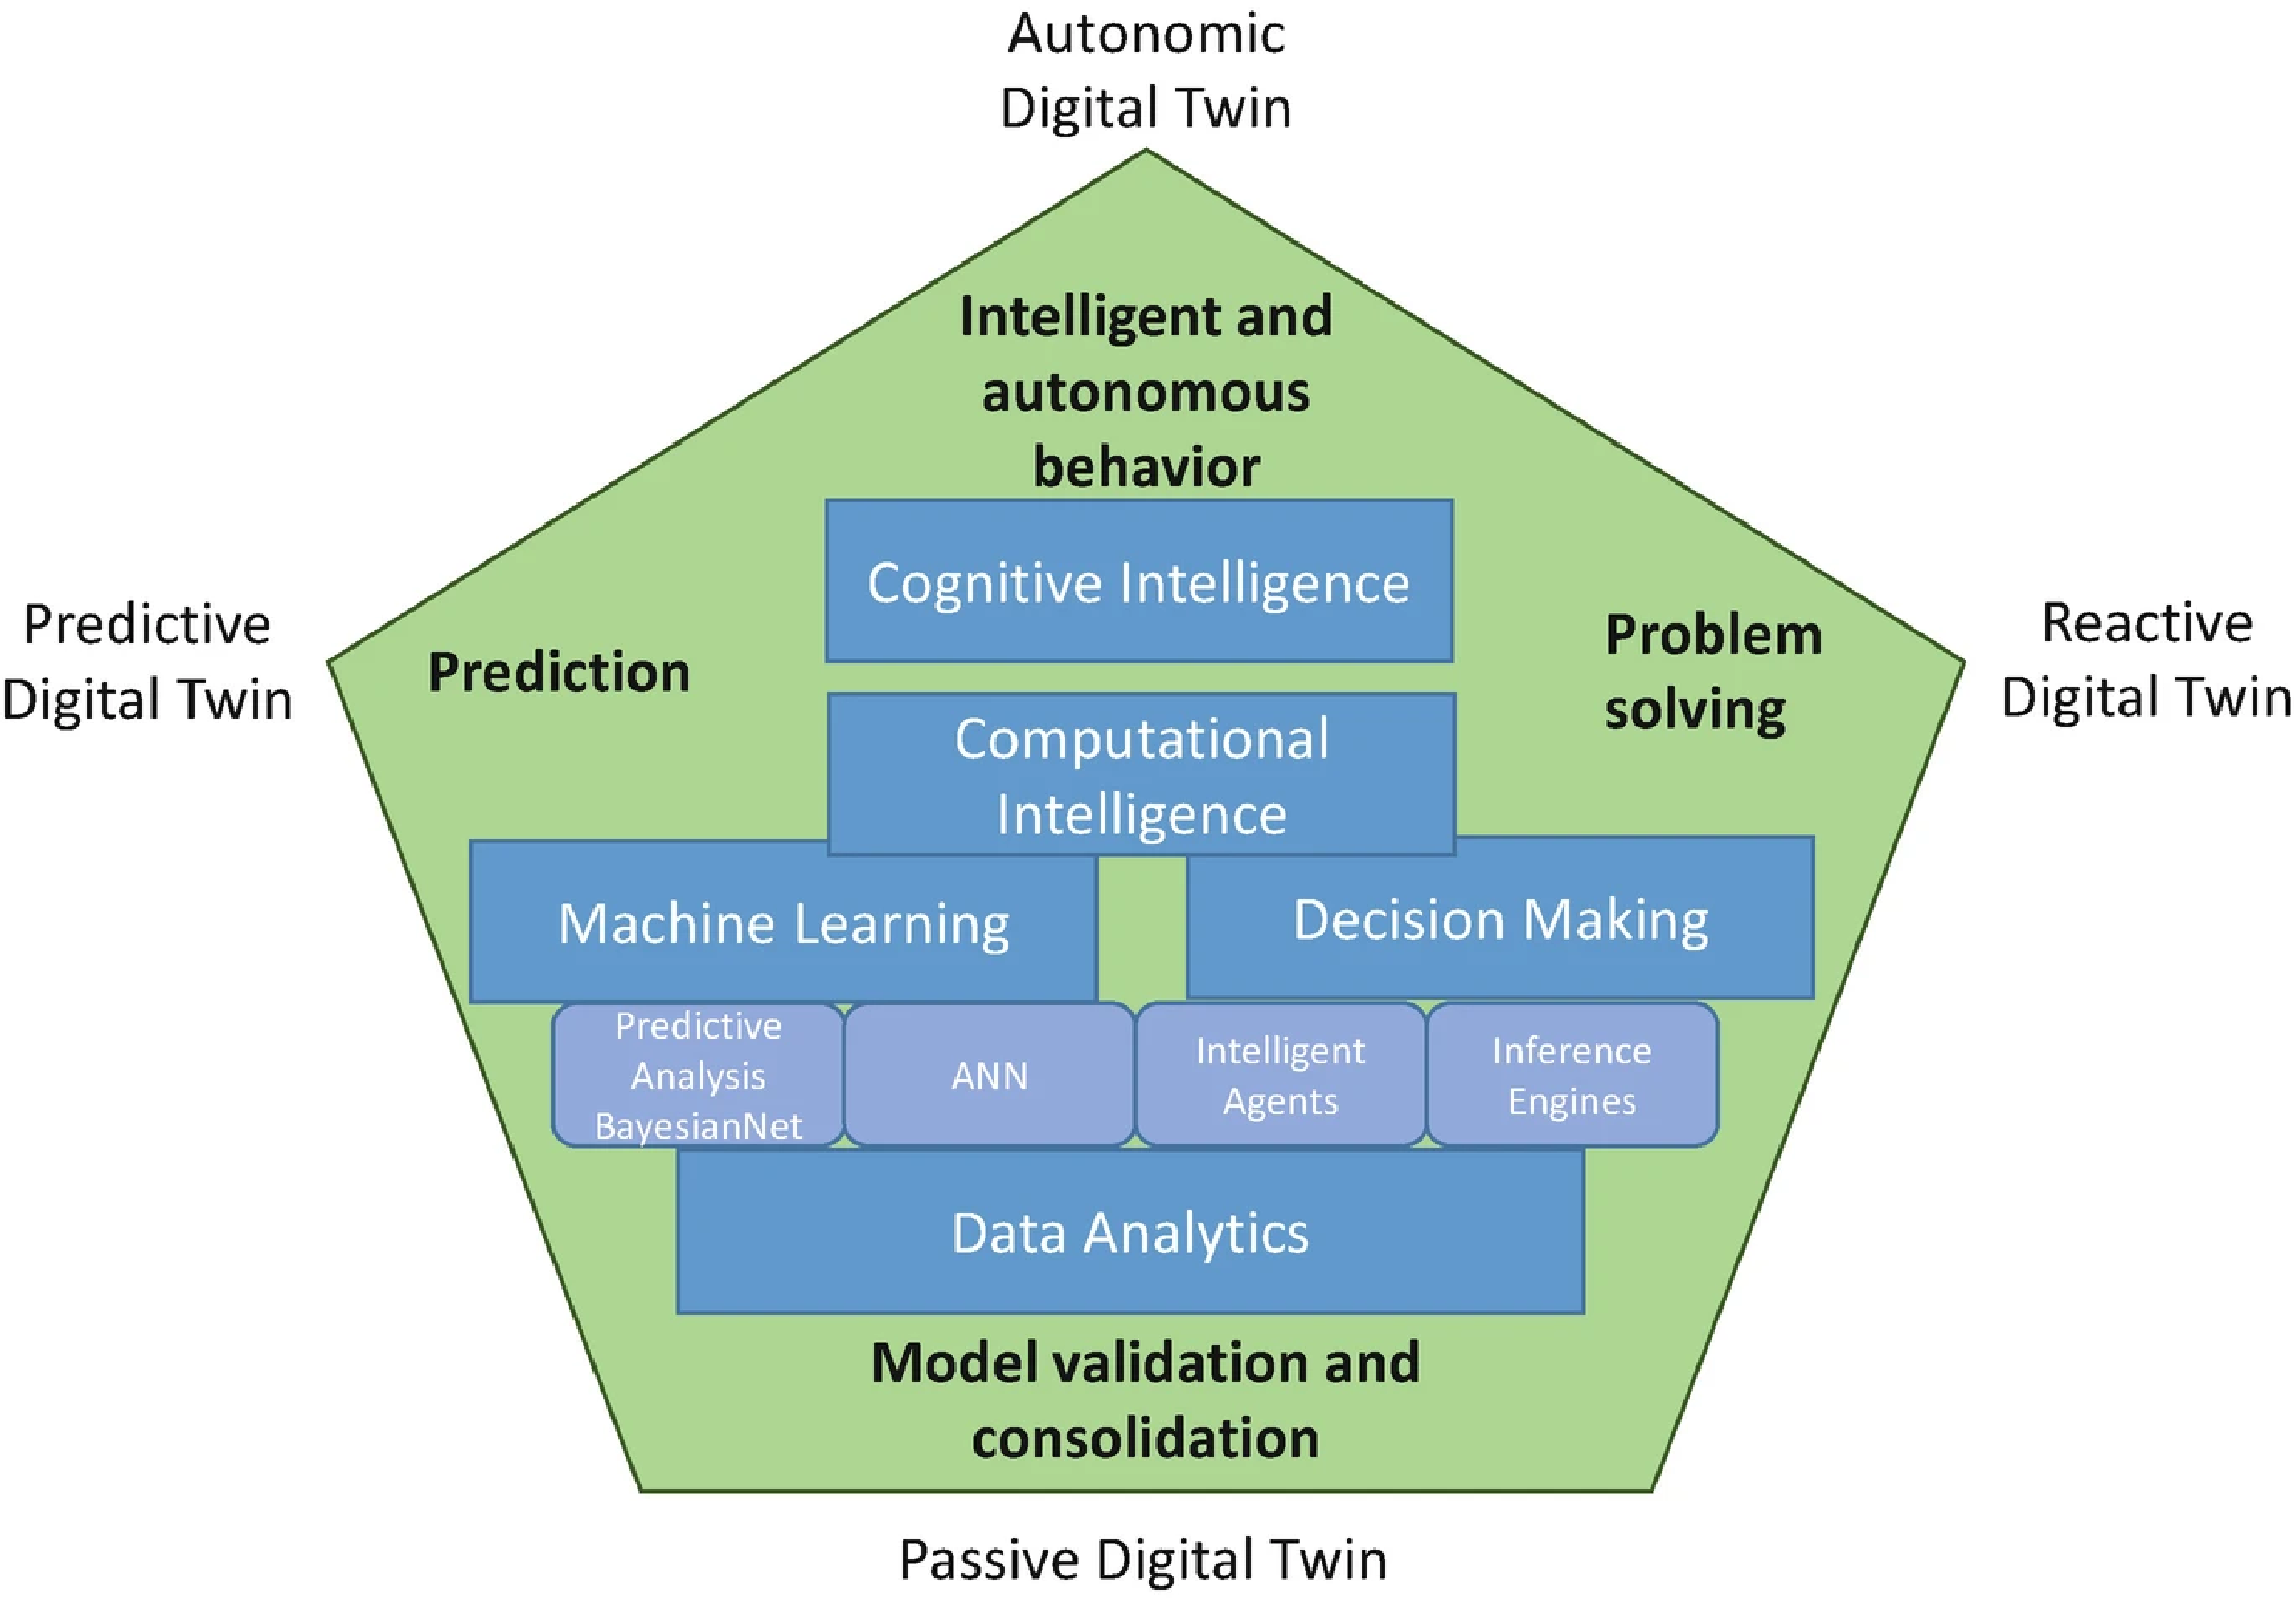
\includegraphics[width=0.9\textwidth]{figures/AI_DT_pentagon.pdf}
    \caption{Artificial intelligence with respect to \ac{DT} capabilities, from \cite{Minerva_Crespi_Farahbakhsh_Awan_2023}.}
    \label{fig:ai-dt-pentagon}
\end{figure}

Passive \acp{DT} can be supported by statistical data analytics techniques to create models of the \ac{PA}. 
%
Predictive \acp{DT} can leverage different techniques such as regression, time series analysis, deep learning but also fuzzy logic to implement the prediction capabilities. 
%
This of course requires the availability of historical data to train such models. 
%
Reactive \acp{DT} can instead use classification techniques, decision-trees and rule-based systems to implement decision-making. 
%
Finally, Autonomic \acp{DT} can combine different reasoning techniques with planning to implement self-adaptation and autonomous beavior.
%
This level of intelligence is often associated with the vision of \emph{Cognitive Digital Twins}~\cite{Zheng_Lu_Kiritsis_2022,Intizar_Ali_Patel_G_Breslin_Harik_Sheth_2021} in which the \ac{DT} has a strong degree of autonomy with respect to its \ac{PA} and can influence its behavior to achieve specific goals.
%
The technologies tied to this vision include knowledge representation, ontologies and reasoning, hence including the more symbolic side of \ac{AI} techniques, rather than only relying on data-driven techniques.

%=======================================================
\section{Digital Twins in Healthcare}
%=======================================================

\acp{DT} have been used to tackle the tracking, prediction and simulation of physical assets in several domains, and in healthcare it is considered a true revolution~\cite{Erol_Mendi_Doğan_2020}.
%
\acp{DT} are seen as a key technology to implement the vision of \emph{Healthcare 4.0}~\cite{Alazab_Khan_Koppu_Ramu_M_Boobalan_Baker_Maddikunta_Gadekallu_Aljuhani_2023} (see ~\ref{chap:back:health4.0}), as they align with the core principles of this new paradigm, promoting digitalization, data integration and proactive and personalized care~\cite{Björnsson_Borrebaeck_Elander_Gasslander_Gawel_Gustafsson_Jörnsten_Lee_Li_Lilja_et_al._2019}.

\begin{figure}
    \centering
    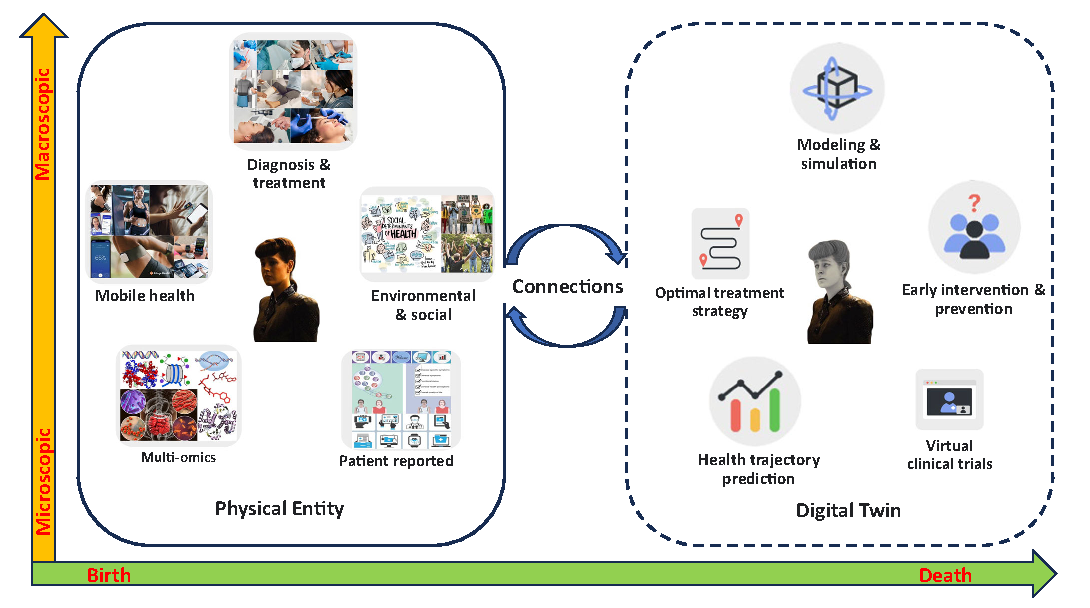
\includegraphics[width=\textwidth]{figures/dt4h_overview.pdf}
    \caption{An overview of \ac{DT} for healthcare, showing enablers and target goals, from \cite{Katsoulakis_Wang_Wu_Shahriyari_Fletcher_Liu_Achenie_Liu_Jackson_Xiao_et_al._2024}.}
    \label{fig:dt-healthcare-overview}
\end{figure}

\acp{DT} can hence be used in various specific healthcare applications, with the common goal of improving the quality and efficiency of healthcare services.
%
\Cref{fig:dt-healthcare-overview} shows a conceptualization of \ac{DT} for healthcare, highlighting how the \ac{DT} can have a role in various healthcare applications.
This is supported by an ever rising trend of scientific publications on the integration of \acp{DT} in healthcare~\cite{Katsoulakis_Wang_Wu_Shahriyari_Fletcher_Liu_Achenie_Liu_Jackson_Xiao_et_al._2024}.

Among the main applications of \acp{DT} in healthcare, the ability to create a \emph{Human \acp{DT}} is one of the most sought after~\cite{Shengli_2021}.
%
The vision is that each person could have a \ac{DT} that holds all its relevant healthcare-related data, including biological, genetic and lifestyle information to provide a comprehensive view of a patient's health status over its entire life. 
%
The vision supports the idea of personalized medicine, where treatments and interventions are evaluated first on the \emph{virtual patient} to assess their effectiveness and possible side effects before being applied to the real patient~\cite{Kamel_Boulos_Zhang_2021,Björnsson_Borrebaeck_Elander_Gasslander_Gawel_Gustafsson_Jörnsten_Lee_Li_Lilja_et_al._2019}.
%
This has been also extended towards processes of drug discovery and development, simulating biochemical reactions and drugs interactions~\cite{Katsoulakis_Wang_Wu_Shahriyari_Fletcher_Liu_Achenie_Liu_Jackson_Xiao_et_al._2024}.

Other applications focus instead of building \acp{DT} of specific organs to better model their behavior and diagnose diseases or detect anomalies~\cite{Erol_Mendi_Doğan_2020}. A primary example of this application is cardiology, as creating a \ac{DT} of the human heart is a complex task with great potential to improve the care of heart pathologies, requiring the combination of mechanical and data-driven models~\cite{Corral-Acero_Margara_Marciniak_Rodero_Loncaric_Feng_Gilbert_Fernandes_Bukhari_Wajdan_et_al._2020}.
%
Such \acp{DT} can be used to understand the medical data collected by continuous monitoring devices for \ac{IoT}-based remote healthcare~\cite{Elayan_Aloqaily_Guizani_2021}.

Moving on from the more ambitious clinical applications of \acp{DT} in healthcare, there is also potential for their use in operational contexts, such as optimizing hospital workflows and resource management.
%
\acp{DT} of hospitals~\cite{Peng_Zhang_Yu_Xu_Gao_2020} can model patient flows, support allocation of resources and staff as well as support classic building management tasks such as energy optimization and maintenance of critical systems. 
%
Similarly, \ac{DT} of medical devices can be used to monitor their status and predict maintenance needs, ensuring availability~\cite{Peng_Zhang_Yu_Xu_Gao_2020}.

Finally, \acp{DT} can be also used to model healthcare processes, such as patient care pathways and clinical workflows~\cite{Ricci_Croatti_Montagna_2022}.
%
This can help to track the ongoing processes, automatically produce medical documentation and identify bottlenecks and inefficiencies to improve the overall quality of care and optimize future planning of activities and investments~\cite{Ricci_Croatti_Montagna_2022}.

Overall, the integration of \acp{DT} in healthcare holds great promise, despite the field being still in its infancy and heavily focused on the creation of simulation models rather than fully connected \acp{DT}. 
%
Significant challenges remain to be addressed, starting from the typical challenges of healthcare systems such as data quality, integration, privacy and security, but also the need of validation of \ac{DT} models to ensure their reliability and accuracy for clinical applications~\cite{Katsoulakis_Wang_Wu_Shahriyari_Fletcher_Liu_Achenie_Liu_Jackson_Xiao_et_al._2024}.

In this thesis, we will focus on the use of \ac{DT} to model healthcare processes and workflows, as a more pragmatic approach to leverage the potential of \ac{DT} in healthcare, while addressing the needs of Healthcare 4.0 healthcare systems.


%=======================================================
\section{Digital Twin Interoperability}
\label{sec:back:dt:interoperability}
%=======================================================

The rapid development of \ac{DT} technologies and the adoption of \acp{DT} in various domains has led to a fragmentation of the field. 
%
Moving on from the technological silos of the early \ac{DT} implementations towards a more service-oriented view of \acp{DT},
it is not surprising that interoperability is emerging as a key challenge for \acp{DT}~\cite{piroumian2021interoperability,Rebelo_Moreira_2024}. 


Interoperability is seen as a necessary condition for \ac{DT} maturity.
In \cite{Klar_Arvidsson_Angelakis_2024} the authors propose a general maturity assessment framework for \acp{DT}. 
\Cref{tab:dt-maturity} summarizes the proposed levels of maturity.


\begin{table}[htbp]
\centering
\renewcommand{\arraystretch}{1.2}
\begin{tabular}{c|p{2.8cm}|p{5cm}|p{4cm}}
\toprule
\midrule
\textbf{Level} & \textbf{State} & \textbf{Requirement} & \textbf{Enabled potential} \\
\midrule
\toprule
1 & Replication of assets & 
Digitization of physical assets and their state at moment of capture (e.g. 2D maps or 3D models) & 
Awareness of assets, rudimentary decision support \\
\hline
2 & Connection & 
Connect processes and models to static data and metadata of level 1 & 
Realistic simulations and asset planning \\
\hline
3 & Synchronization & 
Enrich with timely data (sensors and other IoT technologies) & 
Real-time situational awareness and immersive environments \\
\hline
4 & Interaction & 
Two-way data communication and interaction & 
Remote control of physical assets and processes \\
\hline
5 & Automation & 
Transparent explainable systems with broad control potential & 
Autonomous operations optimization and self-maintenance \\
\hline
6 & Interoperability & 
Highly linkable systems characterized by a high level of standardization, ontology definition, and semantic modelling & 
Joint decision-making among various systems, enhanced system of systems performance \\
\midrule
\bottomrule
\end{tabular}
\caption{Levels of \acl{DT} maturity from \cite{Klar_Arvidsson_Angelakis_2024}.}
\label{tab:dt-maturity}
\end{table}

Authors correlate level one and two to the Digital Model, level three to the Digital Shadow and level four and five to the Digital Twin concepts~\cite{kritzinger2018dtmanufacturing}.
%
Level six, which they identify as the highest level of maturity is tied to interoperability and envisions \emph{Connected Digital Twins} that can interact with each other to provide joint decision-making capabilities. 

In this context, interoperability is hence seen as a key enabler for the realization of \ac{DT}-based systems and integrate the \ac{DT} concept as a \ac{CPS} engineering paradigm. 
%
Accordingly, in \cite{Acharya_Khan_Päivärinta_2024}, the authors survey \ac{DT} literature to characterize interoperability in \ac{CPS} and \ac{DT} systems.
%
\Cref{fig:dt-interoperability-levels} visually summarizes the identified levels of interoperability in six levels: 

\begin{figure}[t]
    \centering
    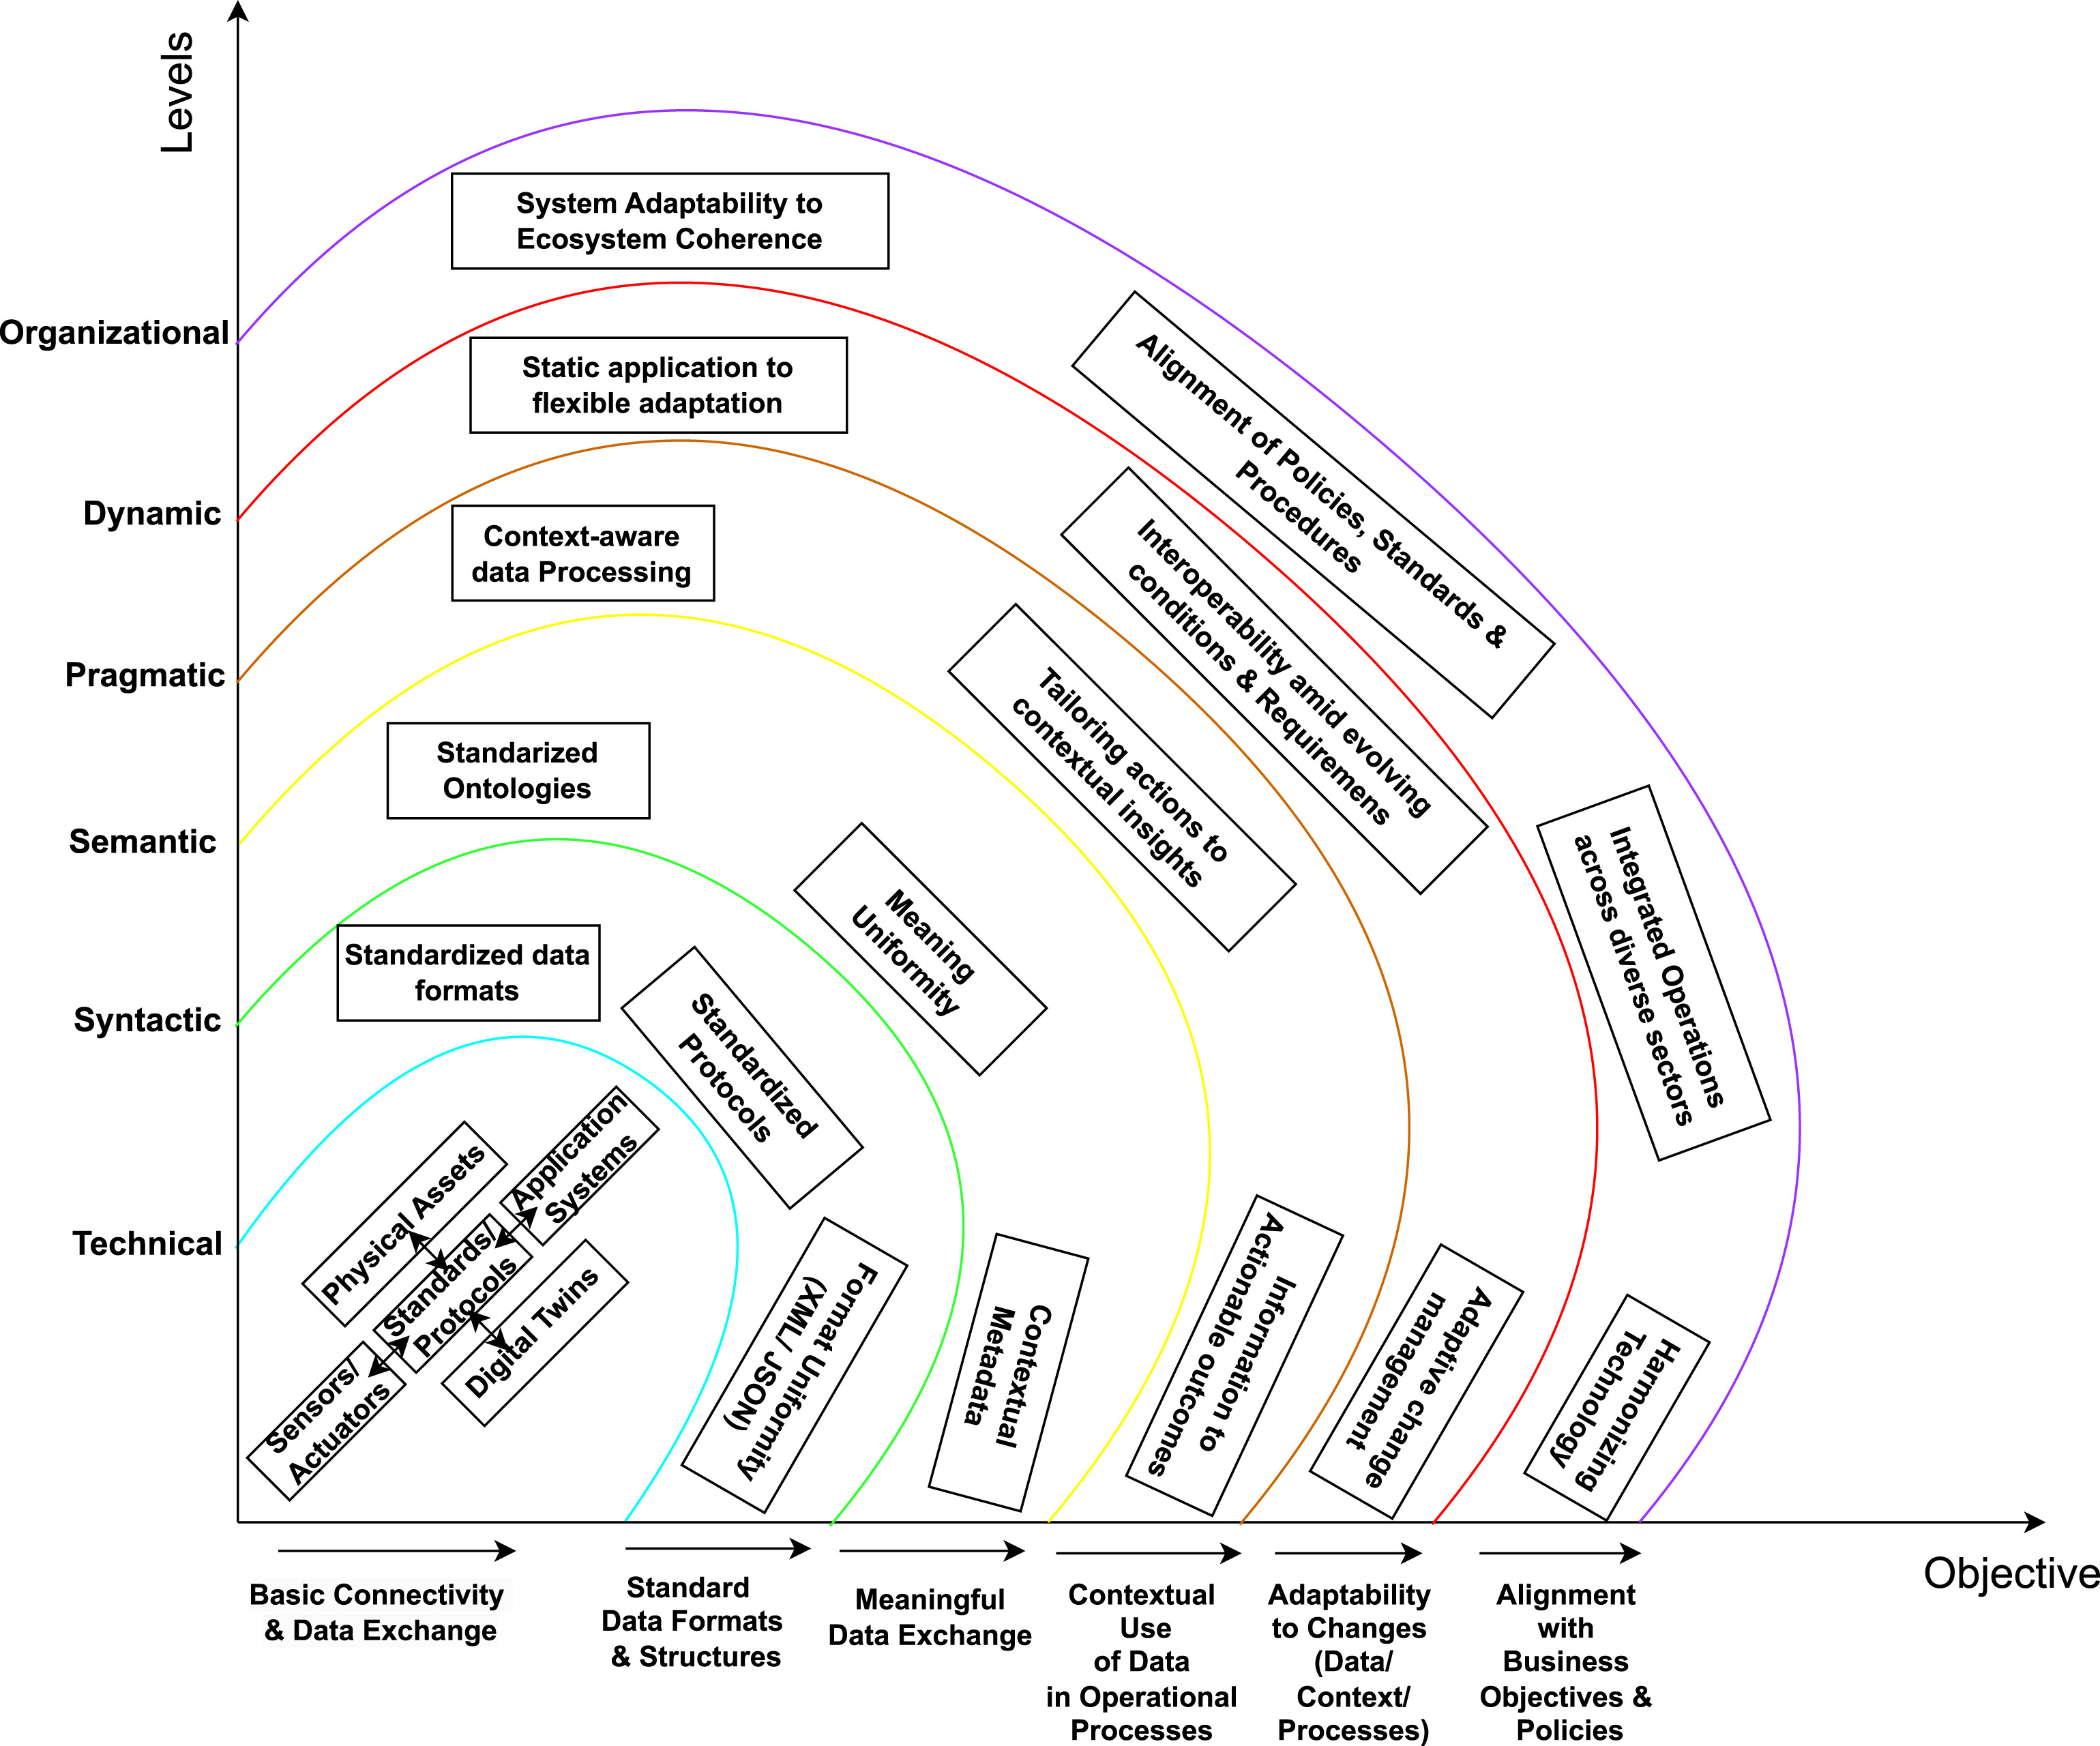
\includegraphics[width=\textwidth]{figures/interoperability-levels.jpg}
    \caption{Interoperability Levels in \acl{DT}, from \cite{Acharya_Khan_Päivärinta_2024}.}
    \label{fig:dt-interoperability-levels}
\end{figure}


\begin{enumerate}
    \item \textbf{Technical Interoperability} is the lowest level and refers to the ability of different systems to communicate and exchange data using common protocols and formats;
    \item \textbf{Syntactic Interoperability} refers to the ability of different systems to understand the structure and format of the exchanged data, enabling them to parse and interpret it correctly;
    \item \textbf{Semantic Interoperability} refers to the ability of different systems to understand the meaning of the exchanged data, enabling them to interpret it consistently;
    \item \textbf{Pragmatic Interoperability} refers to the ability of systems to understand context of the exchanged data and use it to 
    \item \textbf{Dynamic Interoperability} refers to the ability of different systems to adapt and evolve over time, enabling them to maintain interoperability in the face of changing requirements and technologies
    \item \textbf{Organizational Interoperability} refers to the ability of different organizations to work together effectively, through the adherence to standards and the integration of operations. 
\end{enumerate}
%

These studies highlight the importance of interoperability for the future of \acp{DT}, emphasizing the need for standardization and common frameworks to enable seamless integration of \acp{DT} in larger systems. 
%
The envisioned ultimate goal, tends towards \acp{DT} as building-blocks of more complex systems, interacting with each other to provide additional value. 

Of course, there are significant challenges to achieve this vision.
%
In \cite{Klar_Arvidsson_Angelakis_2024}, the authors identify the lack of trust as a key barrier to interoperability, especially for an organizational level as the exchange of data is often perceived as a loss of competitive advantage.
%
Initiatives such as the European data space~\cite{Braud_Fromentoux_Radier_Le_Grand_2021} are trying to address this issue by proposing a federated data infrastructure where data can be shared in a secure and controlled manner.

Other than societal challenges, technical issues such as data silos, proprietary formats, and lack of common standards further complicate interoperability efforts.
%
Standardization initiatives such as the one from \ac{ETSI}~\cite{etsi_TR_103844_v1.1.1_2023} aim to address these challenges by providing guidelines and frameworks for interoperable \acp{DT}.
%
Different challenges arise at different levels of interoperability~\cite{Klar_Arvidsson_Angelakis_2024}.

At the technical level, a plethora of standards originally developed within the industrial \ac{IoT} domain are being proposed to address the communication and data exchange needs of \acp{DT}~\cite{Barnard_2024}.
%
Examples are the \ac{AAS}~\cite{platform_i40_aas_part1_v2}, the \ac{OPC-UA}~\cite{mahnke2009opc}, and \ac{AML}~\cite{DBLP:conf/etfa/DrathLPH08}.
%
These standards, given their different origins and motivations, cover different aspects of a \ac{DT}~\cite{Barnard_2024} and are generally tailored to a specific problem, namely \ac{AAS} focuses on creating a representation of an asset through its static and dynamic properties, operations and services;
\ac{OPC-UA} primarily serves as a secure and efficient \ac{M2M} communication protocol and data model; and \ac{AML} captures the geometry, topology, and behavior of machines in automation processes.


At the semantic level, authors recognize the role of shared semantic models to provide common understanding of the exchanged data.
%
In this setting, ontologies and \acp{KG} are seen as essential tools to implement \acp{DT}~\cite{Karabulut_Pileggi_Groth_Degeler_2024}. They can provide a common vocabulary and shared understanding of an application domain, fostering interoperability, explainability and reasoning capabilities.
%
The survey finds that most \ac{DT} implementations use ontologies to represent the physical layer as it is the one more tied to the application domain. Few leverage ontologies to exchange data and build \acp{KG} to share the \ac{DT} knowledge, limiting their interoperability potential~\cite{Karabulut_Pileggi_Groth_Degeler_2024}.

%
% A different approach to \ac{IoT} interoperability is the aforementioned W3C \ac{WoT} which provides a general purpose model to integrate multiple \ac{IoT} devices, using Web principles to support the discovery of capabilities described through \acp{TD}.
% %
% Differently from the other approaches, the \ac{WoT} focuses on modeling interactions with devices, allowing to translate \acp{API} from machine-specific to Web-based protocols.

% Given the different nature of these standards, they can be viewed as complementary rather than competing against each other.
% %
% There have been integration efforts in order to leverage their different strengths. For instance, \ac{OPC-UA} has been integrated with web technologies~\cite{DBLP:journals/csi/CavalieriSS19} to support direct integration with web clients, operations in \ac{AAS}~\cite{platform_i40_aas_part1_v2} and affordances in \ac{WoT}\footnote{\url{https://profiles.opcfoundation.org/workinggroup/97}} can have an \ac{OPC-UA} protocol bindings, and \ac{AML} specifications can be linked to \ac{AAS} to have a coherent view of the involved assets~\cite{DBLP:conf/etfa/DrathRH19,DBLP:conf/indin/WengerZ018}.
% %
% In this view, the Semantic Web technologies adopted in the \ac{HWoDT} approach can be integrated on top of existing standards and complement their features.

% The Semantic Web excels at general-purpose knowledge representation, and integration of such heterogeneous knowledge under a uniform interface.
% %
% Additionally, it enable reasoning through ontological inference and expressive queries across concepts, supporting use cases that have limited support when using the aforementioned standards alone (see \cref{tab:interop_comparison}, Querying and Data access).
% %
% It is then not surprising that alignment between Semantic Web technologies and industrial standards are being investigated, highlighting similarities between e.g., \ac{OPC-UA}~\cite{DBLP:conf/etfa/MajumderWD19,DBLP:conf/etfa/PerzyloP0K19} and \ac{AAS}~\cite{DBLP:conf/icphys/BedenCB21, platform_i40_aas_part1_v2} data models, to benefit from these features.

%=======================================================
\section{Towards \aclp{DTE}}
\label{sec:back:dt:dte}
%=======================================================

As discussed in the previous sections, \acp{DT} are evolving from the original view of virtual copies of physical products, to serve as a general-purpose engineering abstraction for the strategic design and development of \acp{CPS}.
%
This shift is reflected by both technological advancements with the emergence of \ac{DT} platforms that support the management of multiple \acp{DT}, and the increasing attention to interoperability to enable \acp{DT} to be integrated in larger systems.


Complex \acp{CPS}, in fact, typically consist of interrelated assets whose connections can change dynamically.
%
These relationships are currently difficult to track and model with a single \ac{DT}, hence several approaches are proposing to consider a more collective dimension in which each asset is modeled with its own \ac{DT}, and the overall system is modeled as an \emph{ecosystem} of interconnected \acp{DT}~\cite{web-of-dt-ricci-2022}.
%
\emph{\ac{DTE}}, which are the core concept explored in this thesis, are hence emerging as a key abstraction to address the challenge of effectively model complex \acp{CPS} through a set of interconnected \acp{DT}.
%
The call to \emph{``make more \aclp{DT}''}~\cite{nature_make_moredt} is hence opening a perspective in which \acp{DT} are pervasively used to model strategic \acp{PA} and their interaction becomes crucial to effectively leverage their potential in complex scenarios.

The idea of \ac{DTE} can be traced back to the concept of \emph{Digital Twin Aggregate} introduced by Grieves~\cite{Grieves_2023} which understood the potential of aggregating multiple \acp{DT} instances to derive aggregate insights.
%
In that vision, though, the aggregate was composed of multiple \acp{DT} of the same type of asset, to observe the behavior of different instances of the same product and capture collective trends.

The more modern interpretation of \ac{DTE} can be derived, instead, from the United Kingdom's \textit{National Digital Twin} program~\cite{bulter2018geminiprinciples}.
%
As described in \cite{kendall2021ndt} the National Digital Twin is \emph{``an ecosystem
of digital twins and the protocols by which
they can be integrated securely and
resiliently''}.
%
Finalized at the tracking of the national built environment, the initiative fostered the development of a \ac{DT} integration framework to share and exchange data across different stakeholders.
%
Although the program was focused on a specific domain, the underlying idea of composing an ecosystem of interconnected \acp{DT} rather than a monolithic put forth by the \emph{Gemini principles}~\cite{bulter2018geminiprinciples} can be generalized to other applications.
%
Today, \ac{DTE} are hence envisioned as systems where multiple \emph{different} \acp{DT} are interconnected to model complex scenarios spanning different domains and organizations.

Building on this vision, Ricci et al. proposed the idea of a \emph{\ac{WoDT}}~\cite{web-of-dt-ricci-2022} as a conceptual framework to model \ac{DTE} in an open, distributed and dynamic manner.
The core principle states that:

\begin{quote}
Every strategic \acl{PA} of an organisation must have a corresponding \acl{DT}, mirroring and augmenting its functionalities and services at the digital level, resulting in an ecosystem of connected \aclp{DT}~\cite{web-of-dt-ricci-2022}.
\end{quote}

\todo{Refine the figure to have the layers on the same side}
\begin{figure}[t]
    \centering
    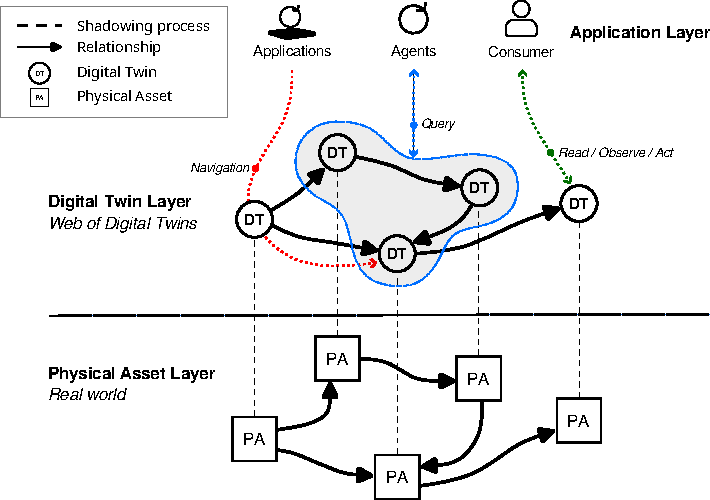
\includegraphics[width=\textwidth]{figures/wodt.pdf}
    \caption{Conceptual model of the \acl{WoDT}.}
    \label{fig:dt-wodt-model}
\end{figure}

The \ac{WoDT} hence strongly emphasizes the service dimension of \acp{DT}, envisioning a pervasive digitalization of the physical world.
%
With this pervasive approach, it becomes essential to manage the relationships between \acp{PA} at the \ac{DT} level through links that connect the corresponding \acp{DT}.
%
From a knowledge representation perspective, the \ac{WoDT} envisions \ac{DT} as entities that expose \emph{domain-level} knowledge.
%
The proposal is to encode such knowledge through semantic models, making it possible to see the \ac{WoDT} as a distributed \ac{KG}.
%
Finally, from an application-oriented perspective, the \ac{WoDT} aims at supporting the discovery, navigation, and exploitation of \acp{DT} and their services to support complex applications that span multiple \acp{DT}.

\Cref{fig:dt-wodt-model} summarizes the conceptual model of the \ac{WoDT}.
%
We can distinguish three main layers:
\begin{itemize}
    \item The \emph{Physical Layer} which includes the \acp{PA} which can be connected by dynamic relationships in the physical world;
    \item The \emph{\acl{DT} Layer} which includes the \acp{DT} that model the \acp{PA}, linked by relationships that reflect the ones in the physical layer;
    \item The \emph{Application Layer} which includes applications, users and possibly autonomous software agents that can interact with the \ac{DT} layer to access \ac{DT} data and services.
\end{itemize}

The resulting holistic conceptualization enables services that extend beyond the boundaries of a single \ac{DT} to encompass the ecosystem as a whole, improving the design of large-scale systems.
%
The application layer implements high-level \acp{API} to expose functionalities to users and applications.
%
These include the possibility to \emph{observe} the evolving state of (subgraphs of) \acp{DT}, as well as to \emph{query} the \ac{KG} to selectively retrieve data from the \ac{WoDT}. 

The \ac{WoDT} proposes a general-purpose metamodel to support a common understanding of \acp{DT} in the ecosystem, fostering interoperability and integration across different application domains.
Hence, each \ac{DT} in the ecosystem is modeled through a set of:
\begin{itemize}
    \item \textit{Properties} that represent the observable attributes of the \ac{PA}, as labelled data that can evolve over time based on the state of the \ac{PA};
    \item \textit{Relationships}: that reflect, at the \ac{DT} level, the connections between the \acp{PA} as links to other \acp{DT};
    \item \textit{Actions}: that represent operations which can be invoked to modify the state or behavior of the \ac{PA};
    \item \textit{Events}: exposing notifications representing domain events of the \ac{PA}.
\end{itemize}

The \ac{WoDT} serves as this thesis conceptual foundation to explore the challenges and opportunities of practically implementing \ac{DTE}. 


%=======================================================
\section{Final Remarks}
%=======================================================

This chapter provides an overview of the research landscape around \acp{DT}, from the historical definition of the concept to the more recent trends leading towards the idea of \ac{DTE}. 
%
This serves the purpose of identifying what is the interpretation of \ac{DT} adopted in this thesis in the broader scope of \ac{DT} research.
%
A \ac{DT} is considered as the software system that implements the \emph{twinning process} to create and maintain a virtual representation of a generic \ac{PA}, providing services to external users and applications.

In this scope, the chapter highlights the essential properties a \ac{DT} should have, as well as the complexity of the technological panorama required to implement \acp{DT}, with a special focus on the relationship between \ac{DT} and \ac{AI}.
%
The service-oriented perspective and the complexity of the many technologies involved, call for a strong emphasis on interoperability, which will be a crucial theme in this thesis to enable \acp{DT} to be integrated in larger systems.

Among the various applications of \acp{DT}, the chapters also provides a deep-dive into the role of \acp{DT} in healthcare, being the target domain explored in this thesis.

Finally, the chapter introduces the idea of \ac{DTE} as a key abstraction to model complex \acp{CPS} through a set of interconnected \acp{DT}, highlighting the \ac{WoDT} as the conceptual framework adopted in this thesis to explore this vision.

%%%%%%%%%%%%%%%%%%%%%%%%%%%%%%%%%%%%%%%%%%%%%%%%%%%%%%%%
\chapter{The Semantic Web and The \acl{WoT}}
\label{chap:back:Web}
%%%%%%%%%%%%%%%%%%%%%%%%%%%%%%%%%%%%%%%%%%%%%%%%%%%%%%%%

In this thesis, we leverage web technologies and standards to build interoperability in \ac{DTE}. 
Accordingly, this chapter provides an overview of the principal Web technologies, standards and architectural patterns and discuss how they build interoperability in heterogeneous systems. 
%
Additionally, we introduce the \ac{WoT} as an example of how web technologies can be applied in the \ac{IoT} context to achieve interoperability. 


%=======================================================
\section{History and Definitions}
%=======================================================


The World Wide Web, or simply, the Web, was initially proposed as an \emph{information management} system by Tim Berners-Lee in 1989 while working at CERN as a way to facilitate information sharing among researchers~\cite{berners1989information,Gillies_Cailliau_2000}.
%
The fundamental intuition of the Web is to apply the concept of \emph{hypertext}~\cite{nelson1967getting}---text containing links to other documents---to a global network of computers, enabling users to navigate and access information seamlessly across different systems through following Web links.
%
This allows to: 
\begin{itemize}
    \item easily add and link new information without requiring changes to existing systems;
    \item access and share information across a distributed network of computers in a location-independent manner.
\end{itemize}

The Web quickly evolved from a private information-sharing system, to a \emph{universe of global accessible information}~\cite{Berners-Lee_1996}
%
To implement this vision, the Web has been built on a set of fundamental building blocks: 
\begin{itemize}
    \item the \ac{URI} scheme for identifying resources on the Web;
    \item the \ac{HTTP} protocol for communication between clients and servers;
    \item the \ac{HTML} markup language for structuring and presenting information.
\end{itemize}
These essential Web architecture components are standardized by the \ac{W3C}, an international organization that maintains and develops open standards to ensure the long-term growth of the Web. The \ac{W3C} defines the Web as:

\begin{quote}
\emph{
The World Wide Web (WWW, or simply Web) is an information space in which the items of interest, referred to as resources, are identified by global identifiers called \acfp{URI}~\cite{wwwarch2004}.
}
\end{quote}

The definition highlights the role of \emph{resources} as the first-class entities composing the Web. 
%
Resources can represent anything, from documents and images, to services, people and physical objects. 

The history of the Web is often divided into three main generations.
%
Web 1.0 refers to the early days of the Web, characterized by static web pages and limited interactivity.
%
In the early 2000s, the concept of Web 2.0 emerged to highlight the shift towards a more dynamic and interactive Web, in which users could not only consume content but also create and share it through social media, blogs, and wikis.
%
The third and current generation, Web 3.0, is often associated with the emergence of structured data, shifting the focus from human consumption to machine-readable representations~\cite{Aghaei_2012}.

The \emph{Semantic Web}~\cite{berners2023semantic} represents a vision for a Web of data that can be processed and understood by machines, enabling intelligent applications and services.
%
The Semantic Web builds on the existing Web infrastructure and introduces new standards and technologies to represent, share, and reason about data in a machine-readable way. 

\begin{figure}[t]
    \centering
    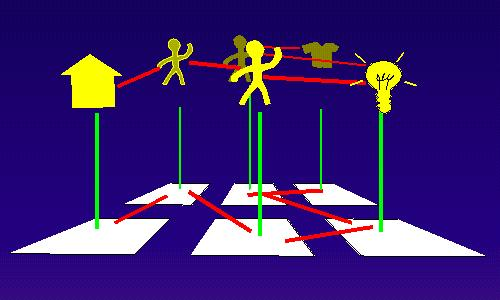
\includegraphics[width=0.8\textwidth]{figures/semantic.jpg}
    \caption{A slide showing the concept of the Semantic Web, with documents linked to real-world concepts through semantics, from \cite{bernerslee1994www94plenary}.}
    \label{fig:semantic-web-idea}
\end{figure}

In its keynote talk outlining future directions for the Web at the 1994 World Wide Web Conference, Tim Berners-Lee discussed the role of semantics on the Web (see \Cref{fig:semantic-web-idea}): 

\begin{quote}
\emph{
But to a computer, it looks kind of flat [...] what it sees is a bunch of documents [...] and in fact we know that there is a world that is being described by these documents [...] but there is no semantics out there [...] the World Wide Web scaled, and it was sufficiently fun for everybody to use, but I missed out on putting semantics in [...] Semantics allow machines to manipulate reality. Well, machines at the moment can browse the Web, but if you put semantics over this then machines basically are browsing through reality~\cite{bernerslee1994keynote}.
}
\end{quote}

Following this original vision, in this thesis we leverage (semantic) Web technologies and standards to build interoperability in \ac{DTE}, with the goal of representing physical reality with machine-readable descriptions through networks of interconnected \acp{DT}.

%=======================================================
\section{The Web Architecture and Hypermedia}
%=======================================================

\todo{Maybe a figure of REST?}

The Web's success is a testament to how its design rationale, open standards, and protocols can enable seamless integration across diverse systems and data sources.
%
The architecture of the Web is based on a client-server model, where clients (e.g, web browsers) request resources from servers (e.g., web servers) using the \ac{HTTP} protocol.
%
This strong separation of concerns allows clients and servers to evolve independently, as long as they adhere to the same protocols and standards.
%
The principles of the Web architecture were formalized by Roy Fielding's PhD dissertation~\cite{fielding2000architectural}, where he introduced the concept of the \emph{\ac{REST}} architectural style.

\ac{REST} is defined by a set of constraints that promote scalability and interoperability in distributed systems. 
%
Constraints include client-server separation with stateless interactions for a strong separation of concerns, a \emph{uniform interface} between the two, cache mechanisms to improve performance and scalability supporting a layered system architecture, and code-on-demand for extensibility of client functionality~\cite{fielding2000architectural}.
%
The \emph{uniform interface} constraint is the cornerstone of \ac{REST}, achieved through:
\begin{itemize}
    \item resources identified by \acp{URI} which can unambiguously reference any entity in the global Web;
    \item manipulation of resources via a small set of methods (e.g., HTTP GET, PUT) for exchanging representations (e.g., JSON, XML) of their current or intended state; 
    \item self-descriptive messages using standard methods, media types, etc.;
    and
    \item server-guided navigation presenting both data and currently available controls using \ac{HATEOAS}.
\end{itemize}

The last point highlights the importance of \emph{hypermedia} in the Web architecture.
%
Although originally coined to extend the concept of hypertext to include multimedia content, Fielding defined hypermedia as:

\begin{quote}
\emph{
Hypermedia is defined by the presence of application control information embedded within, or as a layer above, the presentation of information. Distributed hypermedia allows the presentation and control information to be stored at remote locations~\cite{fielding2000architectural}.
}
\end{quote}

This perspective shifts the focus from merely linking static documents to enabling dynamic interactions and navigation in the Web.
%
This makes the Web not only a repository of information but also an interactive platform for applications and services.
%
The Web's hypermedia nature, in fact, allows clients to discover and interact with resources dynamically, following links and controls provided by servers, rather than relying on fixed, predefined interactions.

The \ac{HATEOAS} sub-constraint of the uniform interface is particularly relevant for supporting the dynamic discovery of resources and actions in the open Web.
%
In a famous blog post, Fielding clarified the importance of \ac{HATEOAS}, explaining that hypermedia is the \emph{``simultaneous presentation of information and controls such that the information becomes the affordance through which the user (or automaton) obtains choices and selects action''}~\cite{fielding2008hypertext}.
%
The Web's hypermedia-driven interactions enable clients to navigate and interact with resources dynamically, following links and controls provided by servers, based on the current context and state of the application.
%
This mechanism further cements the Web as a platform for building interoperable systems that can evolve and adapt over time and that can support automated clients in discovering interactions and adapting to changes.

%=======================================================
\section{Semantic Web Technologies}
\label{sec:back:web:semantic-web-technologies}
%=======================================================

The Semantic Web vision~\cite{berners2023semantic} exploits the hypermedia-based nature of the Web and advances interoperability by introducing machine-readable representations with shared semantics.
%
The Semantic Web is not ``a separate Web, but an extension of the current one''~\cite{berners2023semantic}, as such, it shares the same fundamental building blocks (e.g. \ac{URI}, \ac{HTTP}, \ac{REST}) and extends them with a set of dedicated standards and technologies to represent data in order to be processed and understood by machines.


\begin{figure}[t]
    \centering
    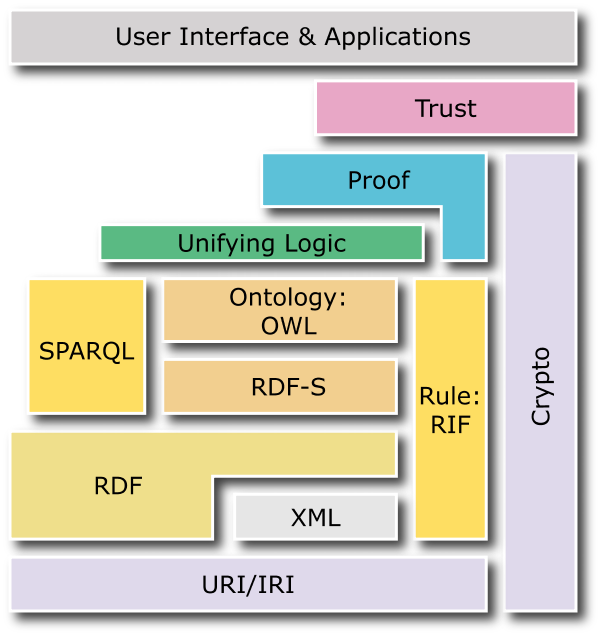
\includegraphics[width=0.8\textwidth]{figures/semantic-web-stack.png}
    \caption{The Semantic Web ``cake'' showing the layers of the technological stack, from \cite{bratt2007semanticweb}.}
    \label{fig:semantic-web-stack}
\end{figure}


\Cref{fig:semantic-web-stack} illustrates the layers of the Semantic Web technological stack with the main standards associated with each layer. 

The foundational building block is the \ac{RDF}, which provides a common data model for representing information about resources on the Web in the form of subject-predicate-object \emph{triples}~\cite{rdf-concepts}.
%
\ac{RDF} triples compose a directed labeled graph, where nodes represent resources and edges represent relationships between them. 
%
Nodes can be either \acp{IRI} (an extension of \acp{URI}) identifying a resource or \emph{literals} representing a typed value (e.g., string, number, date).
%
Additionally, \ac{RDF} supports \emph{blank nodes} to represent resources without a global identifier and support more complex structures than the basic triple structure allow.
%
In its latest version, \ac{RDF} officially supports also having \emph{triple terms} enabling the use of triples as objects of other triples, previously introduced by the {RDF-star} extension~\cite{hartig2021rdfstar}.
%
Predicates of a \ac{RDF} triples are always \acp{IRI}, which ensures a consistent and unambiguous identification of the relationships between resources.
%
Through the combination of these basic elements, \ac{RDF} enables the representation of relationships between resources, which can encode machine-understandable knowledge about a domain.

\ac{RDF} can be serialized in various formats, with the original being an XML-based syntax, while more recent formats include the JSON-LD syntax popular due to its compatibility with JSON-based systems~\cite{json-ld} and \emph{Turtle} syntax, which provides the most compact and human-readable representation of \ac{RDF} graphs~\cite{turtle}.


\todo{Example of RDF triples or figure??}

The next step in the Semantic Web stack is the introduction of vocabularies to provide shared semantics for the terms used in \ac{RDF} graphs.
%
This is essential to ensure that different systems can understand and interpret data with consistent meanings.
%
The concept of \emph{ontology}~\cite{Vickery_1997} is used to refer to a formal definition of concepts and relationships within a specific domain.

The basic vocabulary layer is provided by \ac{RDF} Schema~\cite{rdfs}, which introduces a simple set of terms to define classes and properties. 
%
The more expressive \ac{OWL}~\cite{olw2overview} builds on \ac{RDF} Schema to provide a richer set of modeling primitives.
%
Through \ac{OWL} ontologies, it is possible to establish taxonomies of concepts and inference rules that enable reasoning over the represented knowledge, as well as axioms that can be used to validate data against the defined schema and discover inconsistencies. 

The combination of \ac{RDF} triples and \ac{OWL} ontologies enables the creations of \emph{\acp{KG}}~\cite{KG_Book:21}, creating a structured representation of knowledge through the primitives provided by these standards.
%
\ac{KG} have the benefit of not requiring a predefined schema, creating a flexible and extensible representation of knowledge that can easily evolve over time. 

\todo{Example of SPARQL query?}

Accessing data in a \ac{KG} requires dedicated query languages that can traverse the graph structure and retrieve relevant information.
%
The \ac{SPARQL}~\cite{sparql} is the standard query language for \ac{RDF} data. It is designed to be SQL-like, making it familiar to use for developers used to relational databases.
%
\ac{SPARQL} allows the retrieval of data by matching graph patterns. The result of a query is a list of variable bindings that satisfy the specified pattern. 

The core set of standards presented above simply provides the foundations for the Semantic Web. 
%
Other relevant technologies include validation of \ac{RDF} data by means of matching \emph{shapes} and conditions using \ac{SHACL}~\cite{shacl}, and rule-based reasoning with \ac{SWRL}~\cite{swrl} which extend the inference capabilities of \ac{OWL} with Horn-clause rule logic~\cite{Horn_1951}.

Interestingly, the technologies described above, can be used outside the Web context, for example for building local \acp{KG} to serve as databases for specific applications. 
%
When integrated with the Web architecture and principles, however, they enable the creation of so-called \emph{Linked Data}~\cite{Bizer_Heath_Berners-Lee_2023}.
%
Originally proposed by Tim Berners-Lee in 2006~\cite{berners-lee2006linkeddata}, Linked Data is grounded on four main principles:
\begin{enumerate}
    \item User \acp{URI} as names for things;
    \item Use \ac{HTTP} \acp{URI} so that people can look up those names;
    \item When someone looks up a \ac{URI}, provide useful information, using the standards (e.g., \ac{RDF}, \ac{SPARQL});
    \item Include links to other \acp{URI} so that they can discover more things.
\end{enumerate}

Together, these principles promote the interrelation of \ac{RDF} resources, enabling the creation of a global distributed \ac{KG} that applications can navigate by following and dereferencing \ac{HTTP} \acp{URI}. 
%
In Linked Data, \acp{URI} are used not only to identify documents and web pages, but also real-world entities, concepts, and abstract ideas.
%
The disambiguation between information resources (e.g., documents) and non-information resources (e.g., people, places, physical objects) is achieved through the use of \emph{hash} or \emph{303} \ac{URI} patterns~\cite{cool-uris}.

To complete the consumption and interaction with Linked Data, the \ac{LDP} specification~\cite{ldp} defines rules and best practices on how to apply \ac{REST} principles to the management of \ac{RDF} resources.
%
\ac{LDP} servers expose \emph{containers} of \ac{RDF} resources, that clients can interact with using \ac{HTTP} methods to create, read, update and delete resources. Depending on the type of container, the containment relationship is implicitly or explicitly represented, to ease the discovery of related resources.

The combination of Semantic web technologies and Linked Data principles provides a powerful framework for creating distributed knowledge bases that can be easily shared, integrated and queried across different systems.
%
Of course, the adoption of this approach is not without challenges. 
%
Despite being around for over two decades, the Semantic Web is still far from the original vision of a global Web of data that can be easily consumed by machines~\cite{Hogan_2020}. 
%
Nevertheless, the technological standards and principles described above have been successfully applied and still offer a solid foundation for building open interoperable ecosystems in which data is shared and integrated with clear semantics, supporting automated reasoning and advanced analytics.

\todo{possibly discuss more about challenges and applications}

%=======================================================
\section{The \acl{WoT}}
\label{chap:back:web:WoT}
%=======================================================

Among the domains in which the application of (semantic) Web technologies has been explored to build interoperability, the \ac{WoT} is particularly noteworthy for the scope of this thesis as it emerged to connect physical objects to the Web, and enable their seamless integration through Web principles and standards.

The original vision of the \ac{WoT}~\cite{Wilde_2007,dguinard:wotMashups:2009} was to leverage the \ac{REST} architectural style to integrate physical \emph{Things} into the Web, enabling their interaction and composition through standard Web protocols and formats, rather than relying on proprietary or custom solutions.

The \ac{WoT} original proposal consisted in a \ac{REST} architecture for \emph{Things}, embedding Web servers directly into devices or using gateways to expose their functionalities as Web resources~\cite{Guinard_Trifa_Wilde_2010}.
%
The \ac{HTTP} protocol was used to interact with physical resources using standard methods (e.g., GET, PUT) to retrieve or update their state (e.g., read a temperature sensor, turn on a led).
%
Finally, integrating things into the Web, allowed using Web techniques to discover resources and compose them into applications, for example by using links between resources representing physical devices~\cite{dguinard:phdthesis:2011}.
%
The resulting layered architecture is illustrated in \Cref{fig:wot-layers}, showing how different technologies from the Web and \ac{IoT} domains can be combined to support the creation of applications based on \emph{mashups} of physical \emph{Things}.

\begin{figure}[t]
    \centering
    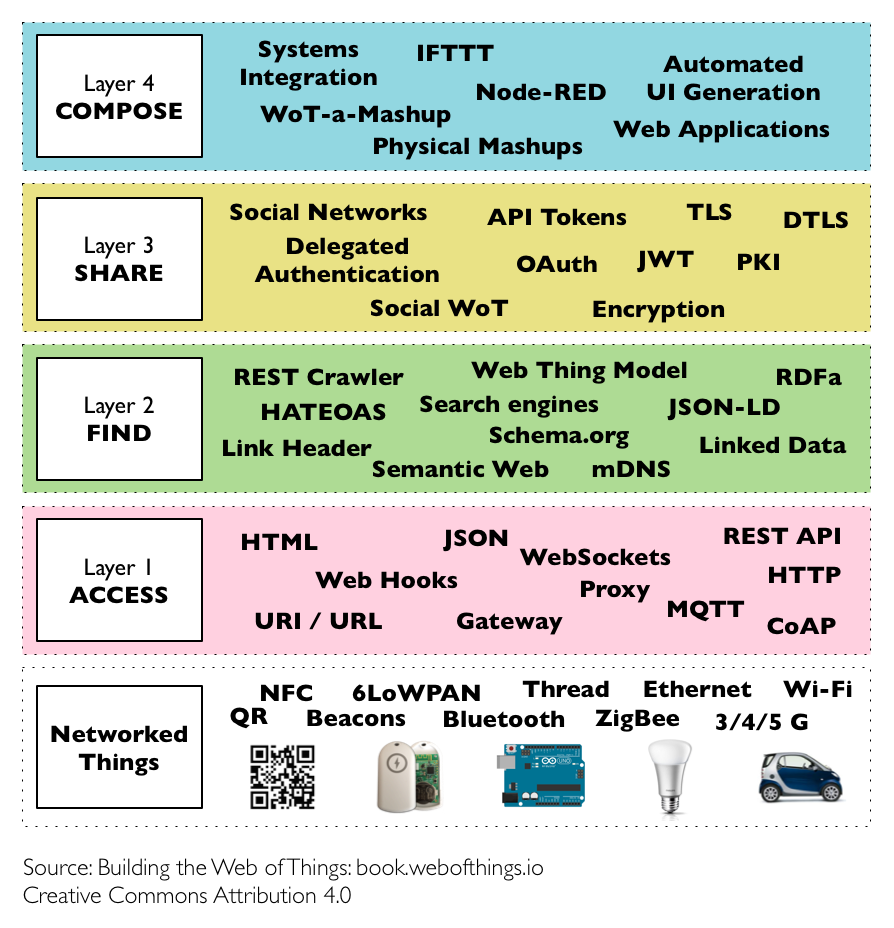
\includegraphics[width=0.85\textwidth]{figures/wot-layers.png}
    \caption{The main layers of the \ac{W3C} \ac{WoT} architecture, from \cite{Guinard_Trifa_2016_book}.}
    \label{fig:wot-layers}
\end{figure}

From its initial proposal, the \ac{WoT} went under a standardization process within the \ac{W3C} resulting in a set of specifications that define the architecture and data model to represent and interact with \emph{Things} on the Web~\cite{wot-arch,wot-td}.


The key component of the \ac{W3C} \ac{WoT} is the \emph{\ac{TD}}~\cite{wot-td}, a machine-readable document that describes the metadata, interfaces, and interaction patterns of a \emph{Thing}.
%
A \ac{TD} describes the capabilities a \emph{Thing} exposes in terms of \emph{interaction affordances}, borrowing from the concept of affordance in design theory which represents what interactions can be perceived from an environment~\cite{Gibson_2014,Norman_2013}.
%
\ac{TD} interaction affordances are of three types: 
\begin{itemize}
    \item \textbf{Properties}, which represent the state of a \emph{Thing} that can be read or written (e.g., the current temperature of a sensor);
    \item \textbf{Actions}, which represent operations that can be invoked on a \emph{Thing} (e.g., turn on a light);
    \item \textbf{Events}, which represent asynchronous notifications that a \emph{Thing} can emit (e.g., a door sensor reporting that the door has been opened);
\end{itemize}
%
Through this simple, yet expressive, metamodel, \ac{TD} can describe a wide range of physical devices with sensors and actuators, supporting both request-response and publish-subscribe interaction patterns.
%
This supports a variety of scenarios for seamless interaction between \ac{TD}-enabled components as showcased in \Cref{fig:wot-arch}. 

\begin{figure}[t]
    \centering
    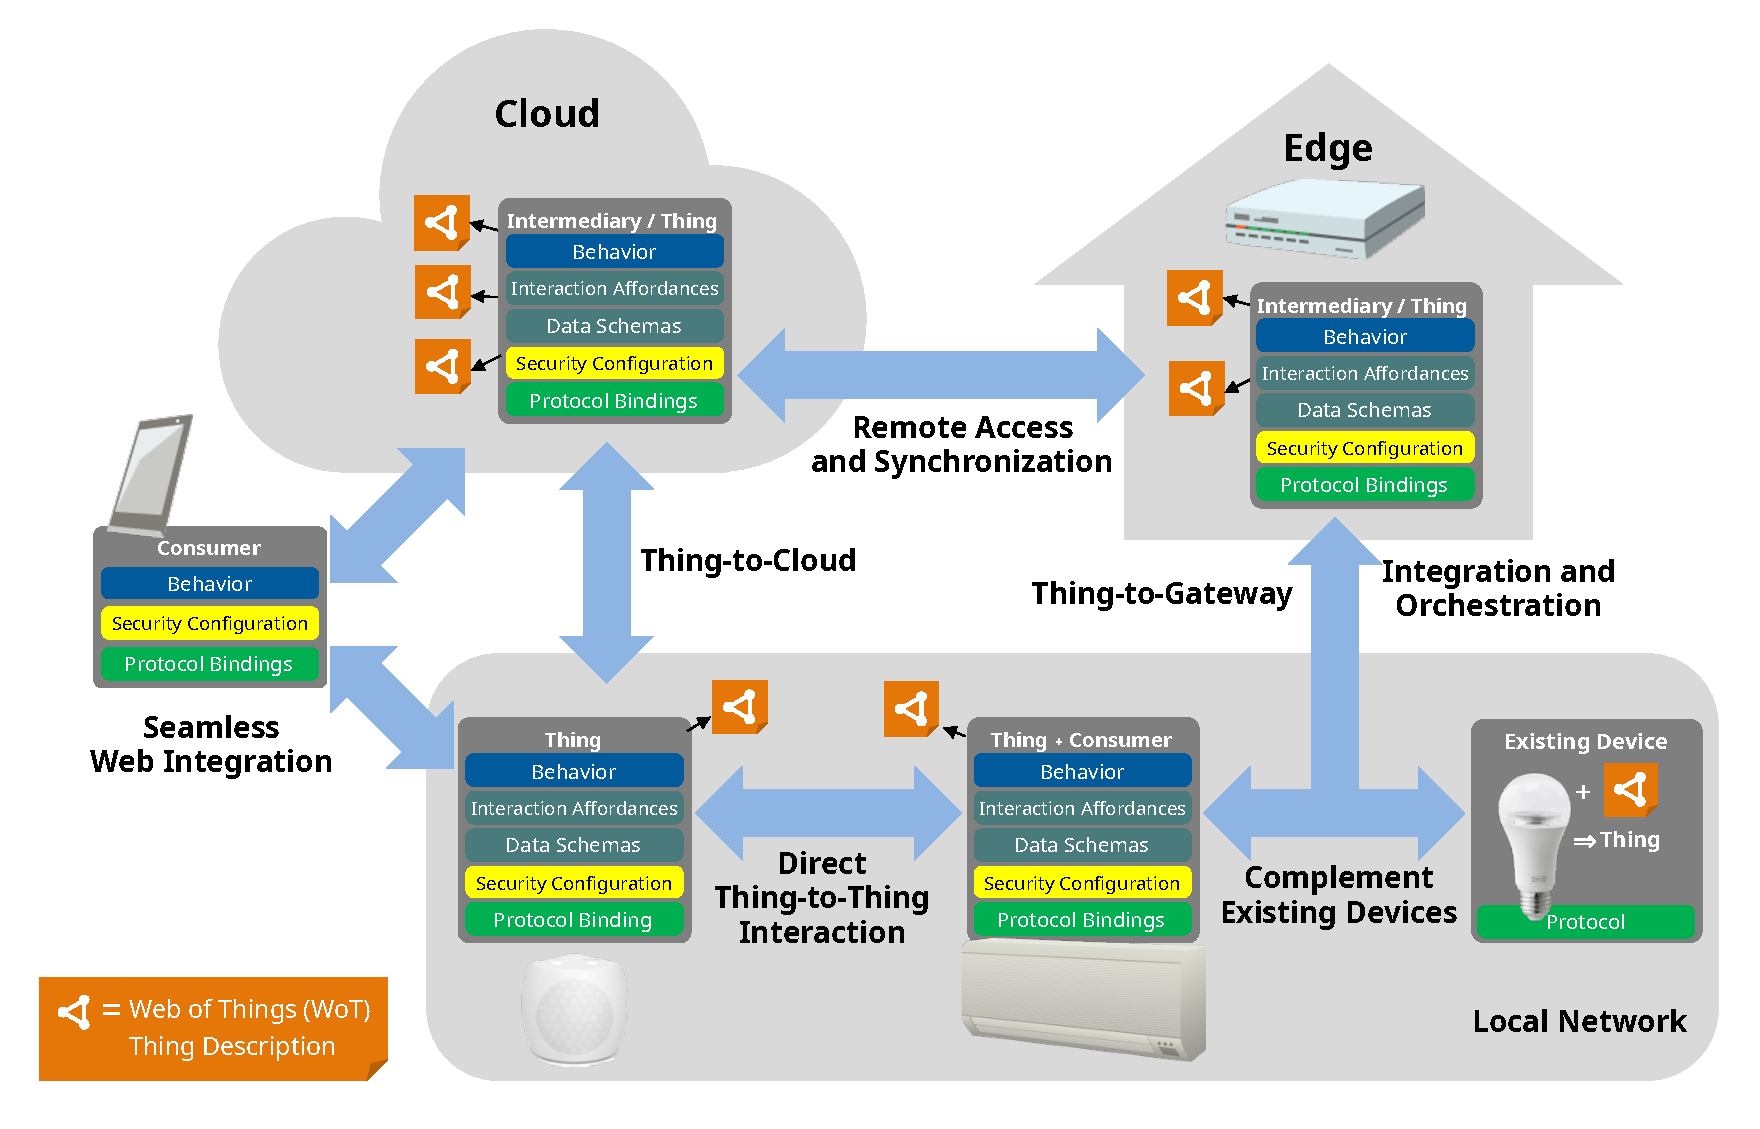
\includegraphics[width=\textwidth]{figures/wotarch.pdf}
    \caption{An overview of the \ac{W3C} \ac{WoT} architecture, from \cite{wot-arch}.}
    \label{fig:wot-arch}
\end{figure}

In the \ac{WoT} architecture, an \emph{exposed} thing represent the logical abstraction of the system component which is capable of responding to interactions as described in its \ac{TD}, hence implementing the behavior behind the exposed affordances. 
%
A \emph{consumer} can discover \acp{TD} through classic Web discovery mechanisms (e.g., search engines, directories), consume them and interact with the corresponding device. 
%
To do this, interaction affordances in a \ac{TD} are associated with \emph{forms}, which specify the data formats for inputs and outputs of a given affordance as well as the \emph{protocol binding} which describes how to actually communicate with the device through one of the supported protocols.

Decoupling the interaction description from the actual protocol binding allows \acp{TD} to possibly support multiple communication protocols and data formats. Examples of supported protocols include \ac{HTTP}, \ac{CoAP}, \ac{MQTT}, and WebSocket, while data formats include JSON, XML, but also binary formats like CBOR~\cite{wot-td}
%
This design ensures that the \ac{TD} can be used in a variety of contexts, and that clients can seamlessly interact with different devices without needing to know the specifics of their communication protocols beforehand. 
%
Additionally, a \ac{TD} interaction affordances can stay the same even if the underlying physical device is replaced or upgraded, greatly improving maintainability and evolvability of systems built using \ac{WoT} principles.

Since the \ac{WoT} is inspired by \ac{REST} principles, \acp{TD} are hypermedia documents. 
%
They hence can include \emph{links} to other resources (e.g. other \acp{TD} of related devices), as well as the aforementioned \emph{forms} that present to consumers the available interactions offered by the \emph{Thing}. 

Finally, \acp{TD} can include security metadata to describe the security mechanisms supported by a \emph{Thing}, such as authentication to secure interaction between consumers and exposed things~\cite{wot-td}. 

The \ac{TD} structure is standardized, and it is usually serialized in JSON-LD, meaning that it is also a valid \ac{RDF} document and is described through a dedicated ontology~\cite{wot-td-ontology,Charpenay_Kabisch_Kosch_2016}.
%
This makes \ac{TD} semantic representations of \ac{IoT} devices, which can be easily integrated with other \ac{RDF} data and ontologies to provide rich descriptions of devices and their capabilities~\cite{Jara_Olivieri_Bocchi_Jung_Kastner_Skarmeta_2014}.

The \ac{WoT} is a successful example of how the transposition of Web principles to a different domain can enable interoperability in heterogeneous systems and support automation in open ecosystems.
%
\ac{WoT} is currently being applied in various domains, including smart homes, manufacturing, smart agriculture, smart cities, and healthcare~\cite{Sciullo_Gigli_Montori_Trotta_Felice_2022}.

Notably, \acp{DT} have been included as an application scenario in the \ac{W3C} \ac{WoT} architecture~\cite{wot-arch}, and there has been work on integrating \ac{DT} and \ac{WoT} technologies~\cite{Jacoby_Usländer_2020,SciulloWoTwins2022} given the close relationship between the two concepts.
%
In this thesis we will explore the intersection between \ac{WoT} and \ac{DT} technologies, investigating how the \ac{WoT} can be used to build interoperable \acp{DT} and \ac{DTE}.

%=======================================================
\section{Final Remarks}
%=======================================================

This chapter introduces fundamental architectural principles and technologies from the Web domain that can be leveraged to build interoperability in open distributed systems.
%
It further presents the \ac{WoT} as an example of how these principles have been applied to the \ac{IoT} domain to enable integration of \ac{IoT} devices under a uniform interface, supported by semantic descriptions of device capabilities.

The principles of the \ac{REST} architectural style, in particular the uniform interface and \ac{HATEOAS} constraints will be explored in this thesis with the twofold goal of:
\begin{itemize}
    \item investigate the application of hypermedia-driven interactions in \ac{DTE} to support dynamic discovery and interaction with \acp{DT};
    \item explore how autonomous agents can leverage such hypermedia-driven interactions to operate in open and dynamic Web environments. 
\end{itemize}
%
The Semantic Web technologies and Linked Data principles will be used to advocate for a shared and machine-readable representation of \acp{DT} and their capabilities, supporting structured knowledge representation and reasoning in \ac{DTE}. 
%
Finally, the \ac{WoT} architecture and \ac{TD} specification will be used as a basis to design and implement interoperable \acp{DT} and \ac{DTE}, exploring how the \ac{WoT} can be integrated with other \ac{DT} technologies to build open ecosystems of interconnected \acp{DT}.

Web technologies and standards hence serves as the \emph{glue} to connect \ac{DTE} with intelligent applications based on autonomous software agents. 


%%%%%%%%%%%%%%%%%%%%%%%%%%%%%%%%%%%%%%%%%%%%%%%%%%%%%%%%
\chapter{\aclp{MAS}}
\label{chap:back:MAS}
%%%%%%%%%%%%%%%%%%%%%%%%%%%%%%%%%%%%%%%%%%%%%%%%%%%%%%%%

%=======================================================
\section{History and Definitions}
%=======================================================

\note{Wooldridge intelligent agents}

\note{Russel and Norvig}

\note{Multi-Agent System definition}

\note{Contextualize Reinforcement Learning Agents}
\note{Possibly even agentic AI?}

%=======================================================
\section{Agent-Oriented Software Engineering}
%=======================================================

%=======================================================
\section{\acl{BDI} Agents}
%=======================================================

%=======================================================
\section{Web-based and Hypermedia \acs{MAS}}
%=======================================================

%=======================================================
\section{\aclp{MAS} and \aclp{DT}}
%=======================================================

%======================================================
\subsection{Synergistic Usage of AAs and DTs}
\label{ssec:synergy}
%======================================================


AAs and DTs are not only used separately 
to deliver intelligent functionalities 
in a mutually exclusive way, 
or as alternative solutions to overlapping requirements.
Their synergistic usage is already seen in the available literature, 
especially in industrial deployments. Here, we briefly report recent surveys that highlight the rich intersection of these research areas.

The contamination of AAs in DTs is mostly related to the need to adopt a variety of artificial intelligence techniques in IoT applications, both to enhance the modelling capabilities of complex assets and to implement automatic controls.
Minerva et al.\ present a classification of DTs in relation to the level of intelligent behaviour the DT exhibits~\cite{Minerva2023}.
They identify the ultimate level of intelligent DT as a proactive (or autonomic) DT, capable of enacting autonomous behaviour based on the physical counterpart's current or future context.
This has a clear link with AAs, that are primarily used to model and encapsulate autonomous and intelligent behaviour in software systems.

Authors of \cite{Pretel2024} deliver a systematic literature review considering both MAS to create DTs and MAS to exploit DTs. 
Table 2 therein highlights how manufacturing is the main use case for synergistic AAs and DTs usage. 
This suggests that Industry 4.0 enabled by IoT technologies is a driving force for AAs and DTs applications. 
Furthermore, Table 3 therein emphasises that 73\% of the surveyed papers do not disclose the AAs and DTs development framework 
and that almost 8\% propose their own 
    (second largest percentage behind a ``team'' of 4 agent-oriented development frameworks). 
This suggests a great fragmentation of uncoordinated proposals, 
generating ``reinvention of the wheel'', especially with respect to the integration of AAs and DTs.

The survey in \cite{10.1115/1.4050244}, instead, has its main focus on DTs considering whether and how AAs (especially MAS) are used to complement the functionalities of DTs. 
Of particular relevance for the present article is Figure 5 therein, 
which reports the vision of an ``Intelligent Product'' (IP) from the literature. 
Such IP fosters the synergistic usage of DTs and AAs. 
DTs help create an ``intelligent being'', 
whereas AAs augment it with an ``intelligent agent'' to make it an IP. 
The ARTI reference architecture is inspired by these concepts, 
and it has been among the first architectures proposed to consider 
the combined usage of AAs and DTs (and the most widely adopted). 
Finally, it is relevant that also here manufacturing and IoT emerge as the main application domains for the integrated usage of AAs and DTs.

The last survey we mention is \cite{Kalyani2025}, 
where the focus is on a one-way integration of AAs and DTs: 
AAs supporting DTs implementation. 
A practical example of such an integration is given in \cite{Latsou2021811}, 
where AAs are used to create a complex DT endowed with ``intelligent'' functionalities (e.g.\ prediction). 
An interesting takeaway that the authors of \cite{Kalyani2025} get from the surveyed literature 
is that a main driving force behind this specific integration is exactly endowment of DTs with AA properties. 
In Section~\ref{sec:abstractions-and-principles} we will see how this need is captured by our principles and proposed micro-architectures for AAs and DTs integration.

Providing the complete overview 
of all the available AAs and DTs-based architectures for IoT scenarios 
is out of the scope of this paper---the interested reader is referred to these surveys. 
However, it may be beneficial for the reader
to report some selected examples.
In \cite{Nie2022}, for instance, 
    an AA is used to aggregate information from different DTs in a manufacturing scenario, 
    to predict faults in machinery and (re-)optimise production scheduling.
Another example in manufacturing is in \cite{Xu2024}. 
    There DTs are used mainly as an abstraction layer over the whole manufacturing system, 
    providing a uniform access layer to AAs. 
    AAs are used mainly to support automatic feedback control (digital to physical) 
    and communication and coordination between robot AAs, task AAs, and workstation AAs.
In \cite{DBLP:conf/pads/ClemenALOOSG21}, instead, 
    AAs are used to build the complex DT of a whole city.

It is also worth noting that there may be literature, such as reference \cite{DBLP:journals/jiii/BiZWL22}, 
where the term ``autonomous agent'' does not appear, 
but whose proposal is well aligned with the literature about AAs. 
For instance, in the mentioned paper, 
a Digital Triad is proposed as an advancement beyond DTs, 
where design knowledge and application-specific intelligence is encapsulated 
in a very similar way to AAs. 
Surveying all of this ``submerged'' literature is a complex task given that terminology likely do not match. 
However, we hope that our contribution can promote cross-fertilisation with these related research efforts, 
in a joint effort to avoid reinventing the wheel---our main motivation for sticking to AAs instead of introducing brand new concepts into DTs.
    
%======================================================
\subsection{Intelligent functionalities for AAs and DTs}
\label{ssec:functions}
%======================================================

The literature on distributing intelligence in IoT discussed in previous sections reports on several intelligent functionalities for which AA and DTs are being actively used by system designers. 
%
We summarise and categorise them here regardless of the specific task they accomplish (e.g.\ time series forecasting vs.\ fault prediction) and of the specific technique adopted (e.g.\ regression, SVM, etc.), but focussing on the \textit{kind} of intelligent function they deliver.
%
This categorisation is useful first of all in defining what we can consider, for the scope of this paper, ``intelligence'' in a practical, bottom-up way, stemming from related works in the area without getting trapped in philosophical arguments. 
%
Then, it is also useful to establish the \emph{coverage} of such functionalities by AAs and DTs, as shown in Figure~\ref{fig:radar-aa-dt}, which already suggests that they can be used synergistically to deliver the full spectrum of such intelligence. 
%
\begin{itemize}
    \item \emph{Prediction}, there including time series forecasting, recommendations, namely any form of reasoning meant to ``guess'' new information based on past and current knowledge. 
    In the IoT, common prediction targets are machinery failures, stock levels, resource use, and system states. 
    \item \emph{Simulation}, encompassing any form of reasoning by hypothesising different states, in the past, present, or future. 
    ``What-if''-like analysis falls into this category. 
    In the IoT, it is common to simulate the future states of individual things, for example, to improve the design of a product or a production pipeline. 
    However, complete systems can also be simulated with an added degree of complexity.%usually integrate multiple AAs and DTs in hierarchical architectures. 
    \item \emph{Planning}, that includes any form of synthesis, and \emph{practical reasoning}~\cite{Bratman1988}, which is meant to figure out how to achieve some practical effect (on the target system) by properly sequencing available actions. 
    Planning to achieve a given system configuration is common in the IoT, as well as planning to reconfigure after some disruptions. 
    \item \emph{Inference}, within which we include both \emph{epistemic reasoning}~\cite{Meyer1995}, that is, synthesising novel information from known data, or data-driven inference such as pattern recognition and classification.
    This is perhaps the most common form of intelligence used in IoT, as even simple monitoring and control applications usually infer situations by aggregating different data coming from distributed sources of information. 
    In addition, fault detection and diagnosis can be gathered in this category. 
    %    \item \emph{Diagnosis} \ste{Tutti}{a pensarci bene è una forma di inference imho, che dite?} \samu{Ste}{La definizione di inference è veramente larga quindi ci cade dentro quasi tutto sì.. io ci ho fatto ricadere anche detection poi nella 4}
    \item \emph{Adaptation} instead gathers all the intelligent functionalities aimed at enabling the system to adapt to unforeseen situations that had not been explicitly managed at design time. 
    As in the previous category, this one is quite broad and includes several heterogeneous approaches, ranging from engineered adaptation (e.g.\ the MAPE-K loop~\cite{Oh2022}) to learning-based methods (e.g.\ evolutionary approaches~\cite{Eiben2005}). 
    \item Finally, we highlight the role of \emph{Learning}, which despite not usually being the primary goal for a functionality, is a valuable tool to implement some of the ones highlighted above and still poses important requirements on the architecture of a system that wishes to support any form of learning process in one of its components.
    That includes statistical machine learning, reinforcement learning, and causal structure learning~\cite{Bordini2020-AI,Erduran2023,Mariani2023a,Mariani2023}. 
    In this category, we group the functionalities that aim to make the system, or one of its components, learn to do something. 
    In IoT, the most common form of learning employs statistical machine learning to create prediction models, for example. 
\end{itemize}
%
The next Section refers to these categories of intelligent functionalities to illustrate why and how to use the design principles proposed therein.


%****************************************************************************************
%****************************************************************************************
\part{\aclp{DTE}}
\label{part:dte}
%****************************************************************************************
%****************************************************************************************

%%%%%%%%%%%%%%%%%%%%%%%%%%%%%%%%%%%%%%%%%%%%%%%%%%%%%%%%
\chapter{Engineering \aclp{DT}}
\label{chap:dte:engineering-dt}
%%%%%%%%%%%%%%%%%%%%%%%%%%%%%%%%%%%%%%%%%%%%%%%%%%%%%%%%

In an attempt to answer \ref{rq:1}, 
this chapter presents a proposal for the engineering of \acp{DT}
focusing on the challenges of integrating heterogeneous sources of \ac{PA} data
and exposing \ac{DT} functionalities as services for digital applications.
%
Additionally, the chapter addresses the challenge of managing the \emph{lifecycle} of a \ac{DT}, 
which is crucial to ensure that the \ac{DT} can accurately reflect the state of the \ac{PA}, 
or signal when it may not be able to do so, in order for applications to make informed decisions on how to 
interpret the data provided by the \ac{DT}.
%
Finally, the modelling of \emph{augmented} functionalities of a \ac{DT} is discussed, with a modular approach
in order to decouple them from the primary \ac{DT} responsibility of \emph{shadowing} the \ac{PA} state. 
%
The resulting contribution is the proposal of an architectural framework and patterns for the engineering of \acp{DT}, 
which has been implemented in a supporting open-source framework: the \ac{WLDT} Java Library\footnote{\url{https://wldt.github.io}}.

%=======================================================
\section{An Abstract Architecture for \aclp{DT}}
\label{sec:dte:engineering-dt:abstract-architecture}
%=======================================================
Starting from the principles outlined by the 5D model~\cite{dt-driven-prognostics-tao-2018},
and incorporating insights from both recent academic research~\cite{web-of-dt-ricci-2022,Bellavista_Bicocchi_Fogli_Giannelli_Mamei_Picone_2023} and relevant standards from industry bodies~\cite{etsi-dt-comm-requirements-2024}.
This section presents a proposal aiming to generalize an abstract architecture that captures the core software requirements for \ac{DT} development.

%%%
\begin{figure}[t]
    \centering
    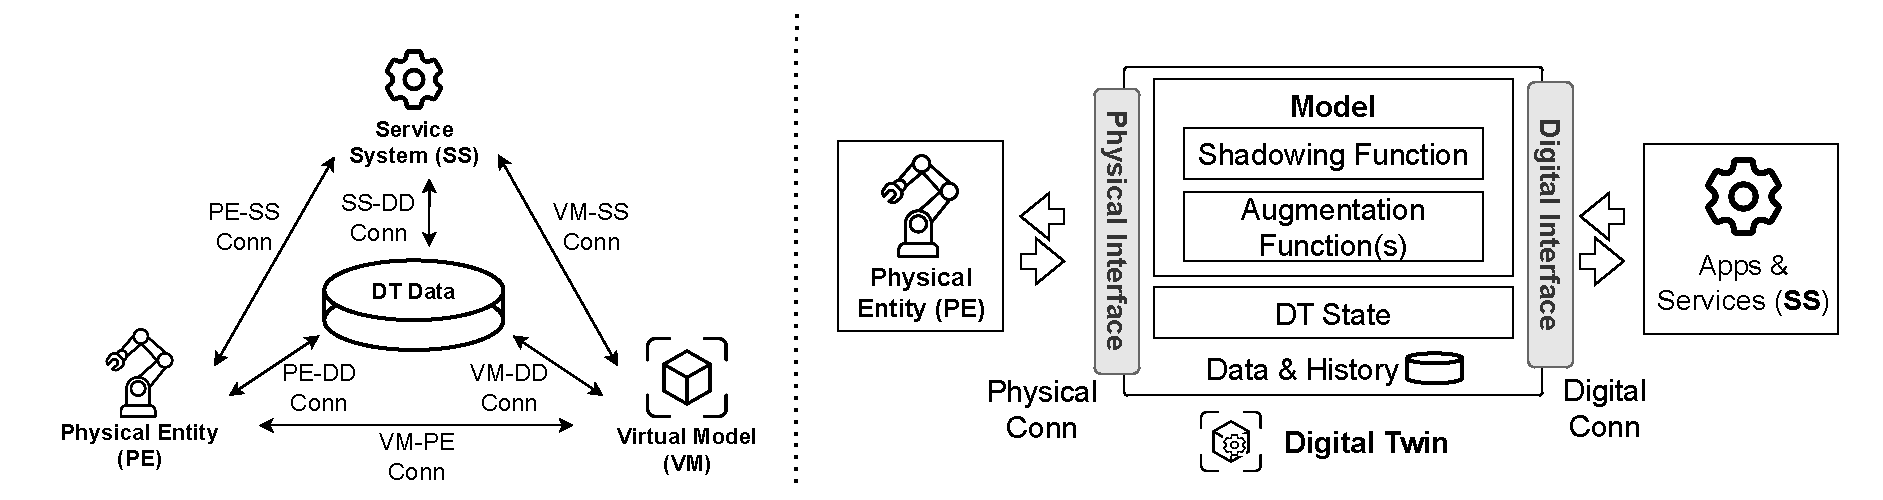
\includegraphics[width=\textwidth]{figures/mapping-Tao-WLDT.pdf}
    \caption{A side-by-side mapping between 5D DT modelling and the abstract \ac{DT} architecture.}
    \label{fig:tao_mapping_dt_modelling}
\end{figure}
%%%

In the 5D model (Figure \ref{fig:tao_mapping_dt_modelling}, left), 
the first dimension, Physical Entities (PE), represents the actual physical object or system being modeled as a \ac{DT}.
The second dimension, Virtual Entity (VE), is the digital representation of the physical entity, replicating its characteristics and behaviors.
The third dimension, Connection (C), ensures linkage between the physical and virtual entities, including communication technologies, data transmission protocols, and synchronization mechanisms for real-time interaction and data exchange.
The fourth dimension, Data (D), covers data management aspects, ensuring accurate and timely data for simulation, prediction, and optimization.
Finally, the fifth dimension, Service (S), involves various services enabled by the \ac{DT}, such as monitoring, simulation, prediction, control, and optimization, leveraging data and insights from the virtual entity to enhance the performance and efficiency of the physical system.

Moving this towards an abstract architectural perspective, a \ac{DT} can be described as the combination of three main high-level components as schematically illustrated in Figure \ref{fig:tao_mapping_dt_modelling} (right): 

\begin{itemize}
    \item \textit{\ac{PI}:} tasked with both the digitalization process and the ongoing synchronization of the \ac{DT} and \ac{PA} throughout their lifecycle based on its characteristic cyber-physical nature and the supported protocols and data formats (e.g., HTTP and JSON, MQTT and binary);
    \item \textit{\ac{DI}:} complementing the \ac{PI}, it manages the routing of \ac{DT}'s internal variations and events directed towards external digital entities and consumers ensuring the \ac{DT}'s interaction, interoperability and observability;
    \item  \textit{\ac{M}:} Defines the \ac{DT}'s behavior through the digitalization process together with augmented functionalities.
    The \textit{shadowing} process is responsible for handling events from both the \ac{PI} and \ac{DI} to model and replicate the state of the asset,
    while \textit{augmentation}~\cite{dt-IoT-context-Minerva-2020} functions extends functionalities of the \ac{PA} through additional features and capabilities supported by the software nature of the twin (e.g., simulation, machine learning inference models).
\end{itemize}


Table~\ref{tab:evaluation} discusses how the proposed architecture supports the core properties of \acp{DT}~\cite{dt-IoT-context-Minerva-2020} compared to both existing research from the scientific literature and features offered by major production-ready platforms.

Among these platforms, general-purpose cloud solutions such as AWS IoT TwinMaker and Microsoft Azure Digital Twins have become prominent.
They provide an integration layer on top of existing cloud data storage and IoT services and hence mainly function as data repositories, storing data from physical assets, with pre-processing handled externally.
%
In such environments, the interaction with the physical world is typically managed using an IoT middleware that collects data and routes it to internal communication buses.
%
These buses are consumed by serverless functions that implement the \ac{DT} model.
Additionally, such cloud platforms often provide digital communication capabilities with built-in visualization, interfaces, and query support.
%
Data acquisition pipelines, supported protocols and data formats are often defined at the platform level, not on a per-\ac{DT} basis, leading to limitations in the shadowing process and client interactions.

Beyond traditional and widely adopted cloud solutions, several industrial platforms are offered by major players like Siemens, General Electric, Bosch, and IBM.
These platforms are often domain-specific and provide strong integration with the physical assets and systems produced by the same companies.
These solutions are tailored to the specific needs of their respective industries, offering robust capabilities for managing and interacting with physical entities.
They do not, though, have a common modeling approach and as such, they offer limited interoperability among the different solutions, as the competitive nature of the market tends to prefer both hardware and software lock-in instead of promoting integration.

In contrast, the proposed approach is \emph{event-driven}, where both the \ac{PI} and \ac{DI} are responsible for capturing events from their respective domains (physical and digital) and forwarding them to the \ac{M} for processing. This allows \acp{DT} to operate as independent software entities, communicating with the external world through finely configurable interfaces.

Following the proposed architecture, a \ac{DT} can be formally represented as:

\begin{equation} 
\label{eq:dt_basic_model}
        DT = \langle PI, M, DI \rangle\\
\end{equation}

Where the \ac{PI} captures data from the \acf{PA}, represented as a stream of time ordered \emph{physical} events $e_{PA}$, and controls physical actuation on the object through time ordered actions $a_{PA}$, 
%
the model \ac{M} encapsulates the \ac{PA} behavior, processes physical events $e_{PA}$, and generates time ordered \emph{digital} events $e_{DT}$,
%
and, finally, the \ac{DI} consumes digital events $e_{DT}$, exposes them to external consumers, and supports the invocation of \emph{digital} actions $a_{DT}$ to modify the behavior of the \ac{PA} through the \ac{DT}.

To better align with multimodel perspectives of \acp{DT}, the model \ac{M} can be actually interpreted as a set of models:

\begin{equation}\label{eq:multi_model}
        M = \{ m_{1}, m_{2}, \dots, m_{n} \} \\
\end{equation}


\begin{table}
\renewcommand{\arraystretch}{1.2}
\centering
\small
\begin{tabularx}{\textwidth}{>{\arraybackslash}m{2.5cm} >{\arraybackslash}X}
\hline
\textbf{Property} & \textbf{Description} \\ \hline

\multirow{2}{*}{\parbox[t]{2.8cm}{\raggedright\arraybackslash\hspace{0pt}\textbf{Representativeness \& Contextualization}}}
& \textbf{Traditional:} DTs are limited to store properties and relationships received from external entities, and do not implement a model or a behavior themselves. DTs fail to encapsulate the PA, and the responsibility of the contextualization is entirely externalized. \\
& \textbf{Event-Driven:} DTs are active entities aware of the characteristics of the PAs through dedicated adapters able to support a fine-grained representation and contextualization thanks to internal models and the event-driven approach. \\ \hline

\multirow{2}{*}{\textbf{Shadowing}} 
& \textbf{Traditional:} The shadowing is not correctly encapsulated within a DT and is dispersed across different components. The constraint to rely on a fixed set of communication protocols and platform-specific data formats creates a strong vendor lock-in, limiting re-usability. \\
& \textbf{Event-Driven:} DT directly encapsulates the functionalities and responsibilities to communicate with the PA through the adoption of any required protocols and data formats and decouples the responsibilities of interacting with the PA through re-usable and interoperable modules. \\ \hline

\multirow{2}{*}{\textbf{Replication}} 
& \textbf{Traditional:} Adoption of centralized and monolithic solutions (e.g., Cloud-only) represents a critical limitation to cross-domain interactions, scalability, and fault tolerance since DTs are designed as passive singleton instances operating in isolated tenants. \\
& \textbf{Event-Driven:} The event-driven approach natively supports the creation of multiple active, independent, and modular DTs interacting by means of events and operating through multi-layered and cross-domain deployments. \\ \hline

\multirow{2}{*}{\textbf{Composability}} 
& \textbf{Traditional:} The composition logic and its management (regardless of whether it is linking or an effective interconnection) are fully externalized, and the DT is passively subject to them. \\
& \textbf{Event-Driven:} Each DT is active and directly handles the composition process through behavior defined by its model, supported by dynamic adapters and a native, event-based notion of observability. \\ \hline

\multirow{2}{*}{\textbf{Augmentation}} 
& \textbf{Traditional:} DT augmentation is a concept entirely missing from state-of-the-art platforms, and it is outsourced to external computational services. \\
& \textbf{Event-Driven:} Augmentation is implemented through a flexible plug-in mechanism allowing the injection of novel functionalities and relying on existing modules to effectively augment the DT. \\ \hline
\end{tabularx}

\caption{Comparison of DT capabilities: limitations of existing (traditional) approaches versus the benefits of the proposed event-driven solution.}
\label{tab:evaluation}
\end{table}

In the proposed approach, the core functionality of the \ac{DT} is the shadowing process, which handles the transformation of data received from the \ac{PI}, feeding the models that characterize the \ac{DT}.
%
The result of the shadowing process is to compute the state of the \ac{DT} $S_{DT}$, which---following the \ac{WoDT} metamodel~\cite{web-of-dt-ricci-2022}---can be represented through sets of: 
\begin{itemize}
\item \textbf{Properties} ($P$): labeled data that change with the evolution of the \ac{PA} state;
\item \textbf{Relationships} ($R$): capturing the existing and dynamic connections among \acp{PA} within the system, mirroring them between the corresponding \acp{DT}; 
\item \textbf{Events} ($E$): non-persistent signals captured by the information gathered from the associated \ac{PA};
\item \textbf{Actions} ($A$): the possible operations that the \ac{DT} allows to be invoked on behalf of the \ac{PA}, to either send feedback to the physical entity or exploit a service exposed by the \ac{DT}.
\end{itemize}

At any given time $t$, the state of the \ac{DT} can hence be represented as: 

\begin{equation}
    S_{DT} = \langle P, R, E, A, t \rangle \\
\end{equation}

Computed states can be stored to maintain a history $H$ of the \ac{DT}, which can be modeled as a time ordered sequence of states:

\begin{equation}\label{eq:dt_history}
        H = \langle S_{DT_1}, S_{DT_2}, ... , S_{DT_n}\rangle\\
\end{equation}

Additionally, to fulfil the \emph{shadowing} process, 
state updates can then be communicated to applications through the \ac{DI}, fulfilling the objective of the \ac{DT} in providing an up-to-date representation of the \ac{PA}.
%
The shadowing process can be represented as a function $Shad$ that given an event from the \ac{PI} $e_{PA}$, the set of models $M$, and the history of previous states $H$, computes the new state of the \ac{DT} and generates an event $e_{DT}$ to be sent through the \ac{DI}:

\begin{equation}
        e_{DT}(S_{DT}) = Shad_{PA \rightarrow DT}(M, e_{PA}, H) \\
\end{equation}

The shadowing is bidirectional:
when actions are invoked, the \ac{DT} receives an action request $a_{DT}$ on its \ac{DI}, validates it through the models $M$ possibly evaluating the history $H$, and then it may propagate the request through its \ac{PI} sending a command $a_{PA}$ to have an effect on the \ac{PA}.

\begin{equation}
    a_{PA} = Shad_{DT \rightarrow PA}(M, a_{DT}, H)
\end{equation}

It is crucial to note that a digital action request does not directly change the state of the \ac{DT}.
Any changes of the state occur only as a result of the propagation of physical changes from the \ac{PA} to the \ac{DT}.
This abstract architectural model addresses the main functional requirements of a \ac{DT}.
It provides a clear separation of concerns between different components focusing on the \emph{shadowing} process as the core responsibility of the \ac{DT} encapsulating the complexity of physical and digital interactions through the \ac{PI} and \ac{DI}. 


Finally, considering these additional specifications, the resulting \ac{DT} model enhances (\ref{eq:dt_basic_model}) to include also the shadowing $Shad$ and the history of states $H$ in the \ac{DT} definition:

\begin{equation}\label{eq:5D_dt_model}
    DT = \langle PI, M, Shad, H, DI \rangle
\end{equation}

In the following sections the abstract architecture will be refined to highlight how it can concretely be implemented to address challenges in \ac{DT} engineering.


%=======================================================
\section{Modular Design of Digital Twin Interfaces}
\label{sec:dte:engineering-dt:physical-digital-adapters}
%=======================================================

As introduced in \Cref{sec:back:dt:interoperability}, interoperability is a key requirement for \ac{DT} development~\cite{Acharya_Khan_Päivärinta_2024,Klar_Arvidsson_Angelakis_2024}.
%
Considering interoperability as the ability to integrate effectively with other system components,
in the \ac{DT} context, such ability can be considered twofold due to their cyber-physical nature.

Figure \ref{fig:dt_application_example} represents a \ac{DT} implemented following the abstract architecture presented in Section \ref{sec:dte:engineering-dt:abstract-architecture} in an exemplary deployment setting.
%
It highlights the role of the \ac{DT} as a bridge between \emph{physical} devices and \emph{digital} applications.

On the one hand, \acp{DT} must effectively integrate with a heterogeneous physical world, interacting with diverse \ac{IoT} devices and systems that operate on different standards, protocols, and architectures.
%
For example machines from different vendors may utilize different communication protocols and interaction patterns.
%
Similarly, in healthcare applications, \acp{DT} must integrate various electronic health records across different data sources, from traditional repositories to sensor networks.
%
This \emph{physical} heterogeneity poses a challenge for the development of \acp{DT}, as, most often, it is unfeasible to modify the existing conditions and the \ac{DT} system must be constructed on top of the legacy ones \emph{adapting} to their requirements.

On the other hand, although \acp{DT} could work in isolation, they are increasingly being envisioned as part of complex software systems.
%
Thus, \acp{DT} needing to integrate with different kinds of services ranging from system automation tools, to data platforms, machine learning pipelines and visualization tools, may expect to face several degrees of \emph{digital} heterogeneity.
%
As for the physical realm, the \ac{DT} might need to \emph{adapt} to the requirements of the digital ecosystem it is part of.
%
Additionally, the modeling of complex \ac{CPS} can be tackled through the idea of \acp{DTE}~\cite{web-of-dt-ricci-2022} which envision multiple connected \acp{DT}, each modeling individual entities of the same domain. 
Such \acp{DTE} can benefit from standardized interactions between \acp{DT} and with higher-level services.

\begin{figure}[t]
    \centering
    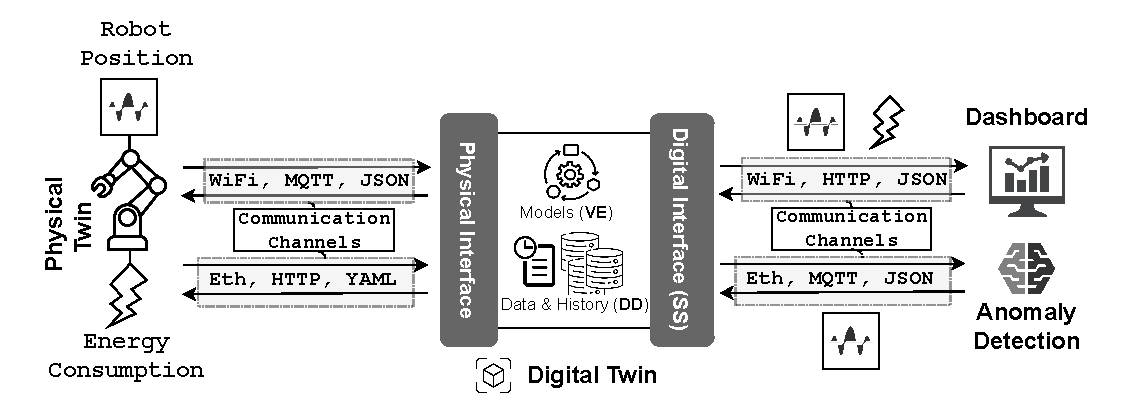
\includegraphics[width=\columnwidth]{figures/dt_application_example.pdf}
    \caption{Example of a DT in an application scenario interacting with a physical asset and digital applications through its PI and DI.}
    \label{fig:dt_application_example}
\end{figure}


Tackling such twofold interoperability challenges requires on one side
the adoption of common data models, semantic interoperability frameworks, and compliance with industry standards~\cite{etsi-dt-comm-requirements-2024} such as OPC-UA\footnote{OPC-UA: \url{https://opcfoundation.org/about/opc-technologies/opc-ua/}}, oneM2M\footnote{oneM2M: \url{https://www.onem2m.org/}}, ISO-23247\footnote{ISO-DigitalTwin: \url{https://www.iso.org/standard/81442.html}}, or the W3C Web of Things\footnote{W3C WoT: \url{https://www.w3.org/WoT/}}.
%
On the other side, the \ac{DT} architecture should accommodate physical and digital heterogeneity \emph{by design} to avoid being locked down in those situations where adherence to a single standard can not be enforced.
Without such measures, \acp{DT} risk becoming fragmented, limiting their ability to collaborate and exchange information across different platforms and applications.
%
The proposal of modular \ac{DT} interfaces aims to address these concerns
at the architectural level, to enhances the interoperability and re-usability of \ac{DT} components in cyber-physical applications.

At an appropriate abstraction level, a \ac{PA} may be digitalized by obtaining and sending data through possibly \emph{several} different \texttt{Communication Channels} (\Cref{fig:dt_application_example}), which 
encompass network protocols, data formats, and physical connections.
The \ac{PI} manages interactions with the \ac{PA}, integrating such channels.
%
Similarly, on the digital side, the \ac{DT} supplies data and insights to applications via the \ac{DI}, adapting to different protocols and representations.

Engineering the \ac{PI} and \ac{DI} requires addressing the challenge of effectively integrating such heterogeneous communication channels.
%
To ensure flexibility and adaptability, it is essential that the core of the \ac{DT}, including its models and implemented behaviors, remains decoupled from the heterogeneous physical and digital communication channels.
%
The \ac{DT}'s shadowing process should focus solely on understanding the available physical data, receiving and transmitting telemetry information, and executing action requests, with no concern for the underlying implementation details.

The remainder of this section describes a proposal for the design the \ac{DT}'s \ac{PI} and \ac{DI}, refining and extending the conceptual model originally proposed in \cite{web-of-dt-ricci-2022} with a concrete implementation based on the concept of modular \emph{adapters}.

%..........................................................
\subsection{Physical Interoperability}
\label{ssec:dte:dt-engineering:physical_interoperability}
%..........................................................

\begin{figure}
    \centering
    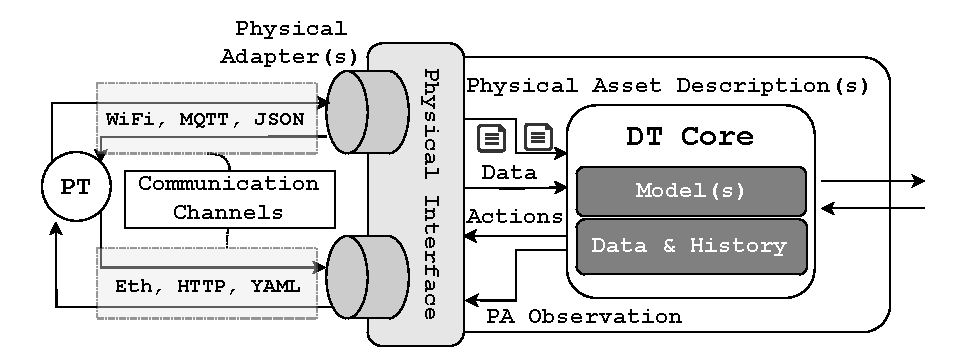
\includegraphics[width=\columnwidth]{figures/dt-interoperability/dt_interoperability_physical.pdf}
    \caption{PI design with modular physical adapters each producing the corresponding \acl{PAD} that is processed by the \ac{DT} Model.}
    \label{fig:physical_interoperability}
\end{figure}


One of the main challenges in facilitating effective communication through the \ac{PI} is the wide variety of communication protocols and data formats used by \acp{PA}.
%
While it can be the case that one \ac{PA} is directly sending all the data concerning its digitalization through only one channel,
it is far more common to build a \ac{DT} aggregating different sources of information~\cite{qi2018dt-and-bigdata}.
%
\ac{IoT} protocols often differ considerably based on the manufacturer, device type, or application domain, making it difficult for the \ac{DT} software to integrate diverse assets.
%
Arguably, the modularity of the \ac{PI}, which encapsulates these responsibilities, is a crucial factor in the design and implementation of interoperable \acp{DT}.
%
Accordingly, the proposal is to design the \ac{PI} as a composition of multiple \emph{\acp{PhA}}: specialized modules capable of interacting with the \ac{PA} using diverse protocols and data formats.
%
As shown in Figure \ref{fig:physical_interoperability}, each \ac{PhA} is responsible for mediating the bidirectional interaction through a single communication channel, simplifying the design and reusability of the component, and making it configurable to adapt to different application contexts.
%
The responsibility of the \ac{PI} becomes then to manage the different \acp{PhA} and make sure the \ac{DT} model can accurately interpret, process, and leverage the data generated by the physical world to create the digital replica and implement its behaviors.
%
Note that although terminology of \ac{PhA} is borrowed from \cite{web-of-dt-ricci-2022}, where it is originally introduced, the \emph{Physical Asset Adapter} proposed in \cite{web-of-dt-ricci-2022} is in fact a conceptual monolithic component, whereas in this concrete proposal a \ac{PhA} is considered as a single-responsibility module of a potentially more complex \ac{PI}.

\subsubsection{Generating \aclp{PAD}}
To facilitate managing different \acp{PhA}, the concept \emph{\ac{PAD}} is introduced: a representation of the capabilities provided by a communication channel in terms of \emph{properties}, \emph{actions}, \emph{events}, and \emph{relationships} that characterize the associated \ac{PA}.
%
Each \ac{PhA}, since it encapsulates the characteristics of a channel, can generate the corresponding \ac{PAD}, effectively decoupling the asset's functionality from the specific communication protocols used.
%
The implementation of the \ac{PAD} generation can be challenging due to the varying capabilities of different communication protocols.
For instance, protocols like \ac{CoAP}~\cite{RFC7252} often come with built-in description and discovery functionalities, which can simplify the process of creating a \ac{PAD} by providing standardized representations of the physical asset's capabilities and behaviors.
On the other hand, protocols like \ac{MQTT}~\cite{MQTTv5} may require developers to add additional information manually to define how information is structured and exchanged, as they do not natively include asset metadata.
In the case of custom or proprietary protocols, the challenge becomes even more pronounced, as these protocols are tailored to specific systems and may lack any standardization or descriptive capabilities.

In all the aforementioned scenarios, the mechanism of \ac{PAD} generation offers a way to encode knowledge about the \ac{PA} bridging the gap by interpreting and extracting relevant information from the protocol used in the associated communication channels.
%
Confining this complexity within the \ac{PI} allows the \ac{DT} model to be agnostic with regard to the complexity of the underlying physical world.

The \ac{PAD} allows the \ac{PI} to discover, extract, and manage asset information and present it to the model that can choose which ones are relevant for the implementation of the \ac{DT} behavior.
%
For example, to create the \ac{DT} of a temperature sensor streaming binary data on MQTT, the \ac{PI} could be composed of a generic MQTT adapter, configured to correctly parse the payload as a decimal number, and generate a \ac{PAD} which advertise the available temperature property to the \ac{DT} model as a Celsius value. 


\subsection{Digital Interoperability}
\label{sec:digital_interoperability}

%%
\begin{figure}[t]
    \centering
    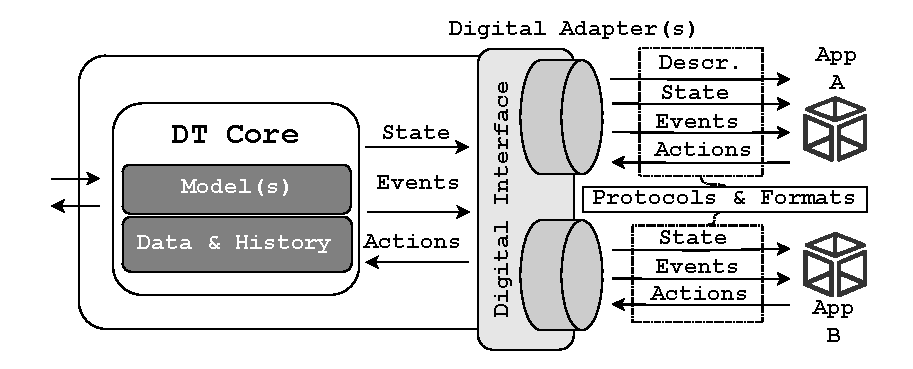
\includegraphics[width=\columnwidth]{figures/dt-interoperability/dt_interoperability_digital.pdf}
    \caption{Digital Interface design with modular adapters and DT description.}
    \label{fig:digital_interoperability}
\end{figure}
%%

As \acp{DT} are meant to bridge between the physical and digital spaces,
interoperability is not only a matter of interfacing with heterogeneous devices, but also other digital applications.
Indeed, despite their initial conception as vertical silos, the concept of \ac{DTE} (\Cref{sec:back:dt:dte}) is emerging to support the the digitalization of complex scenarios through a combination of several \acp{DT}.
%
In this context, \acp{DT} can be used \emph{as-a-service} by other applications implementing the business logic by spanning across different software entities.

To foster interoperability in \acp{DTE}, \acp{DT} must then expose either a standardized general purpose \acf{DI} that can serve different applications or
---following the same design principles adopted to address physical interoperability---
have a modular interface that can satisfy the different needs of different applications
as shown in Figure \ref{fig:digital_interoperability}.

As for \ac{PhA} the terminology is borrowed from \cite{web-of-dt-ricci-2022} and consider to have a \ac{DI} composed of modular \emph{\ac{DiA}}.
The original abstract concept of \ac{DiA} is hence refined to represent a modular component of a more complex \ac{DI}.
Using the concept of \ac{DiA}, the \ac{DI} can expose the \ac{DT} state and services supporting multiple data formats and interaction patterns.
This can be beneficial for integrating it with applications and, especially, legacy systems.
The existence of legacy applications usually implies having little control over the integration requirements, making having more flexible \acp{DT} beneficial to better integrate with the application requirements.

Using several \ac{DiA}, a \ac{DT} could, for instance, support both request-response and publish-subscribe mechanisms to access its current and previous states, support different query languages to access the same data store, expose its current state using different representation formats, etc.
%
This would make the development of the application simpler because adding an application-specific \ac{DiA} won't require intervention in the underlying physical system. 
%
Additionally, the developed application would be more robust and stable since it would depend only on the \ac{DT}, and changes to the physical configuration of the \ac{PA} (e.g., software updates, sensor replacement, network reconfiguration) would have no impact on the application software.
%
Even if the \ac{PA} were to change, (e.g., a software update on a robot changes the telemetry format) the \ac{DI} of the \ac{DT} could stay the same, as the changes would occur within the boundaries of the \ac{PI} and \ac{DT} model.
%
Through this mechanism, \acp{DT} effectively achieve their bridging role, shielding applications from the complexity of physical deployments.

\subsubsection{Describing \aclp{DI}}

A further level of interoperability is possible when allowing \acp{DT} to describe their \ac{DI}, advertising capabilities and available communication channels that applications can exploit.

This is especially relevant in contexts where applications are not bound to a specific interface but can instead process machine-readable descriptions of \acp{DT} and choose to interact with specific assets.
%
A \ac{DT} could then use a \emph{\ac{DTD}}, which, similarly to the \ac{PAD}, can represent the features of the \ac{DT} to its observers.
%
The idea of exposing \acp{DTD} is somewhat present in the major platforms supporting the creation of \acp{DTE}, such as 
Microsoft's \azureTwin{}\footnote{\azureTwin{}: \url{https://azure.microsoft.com/en-us/products/digital-twins}} and \ditto{}\footnote{\ditto{} \url{https://eclipse.dev/ditto/}} and is advocated by standardization activities on interoperability in \acp{DTE}~\cite{etsi-dt-comm-requirements-2024}.

The way such descriptions are implemented may differ significantly, but essentially, they should at least allow representing the \ac{DT}  features and APIs to access them.
%
Notably, differently from the \ac{PAD}, the \ac{DTD} is targeted to external consumers, hence, it should preferably adhere to standard formats and representations to be useful in practice in achieving interoperability.
%
To this end, using Semantic Web technologies (see \Cref{sec:back:web:semantic-web-technologies}) could be a possible solution to implement standard machine-readable \acp{DTD}.
\todo{add forward ref to semantic web descriptors sections}

% \begin{figure*}[t]
%     \setlength{\belowcaptionskip}{-13pt}
%     \centering
%     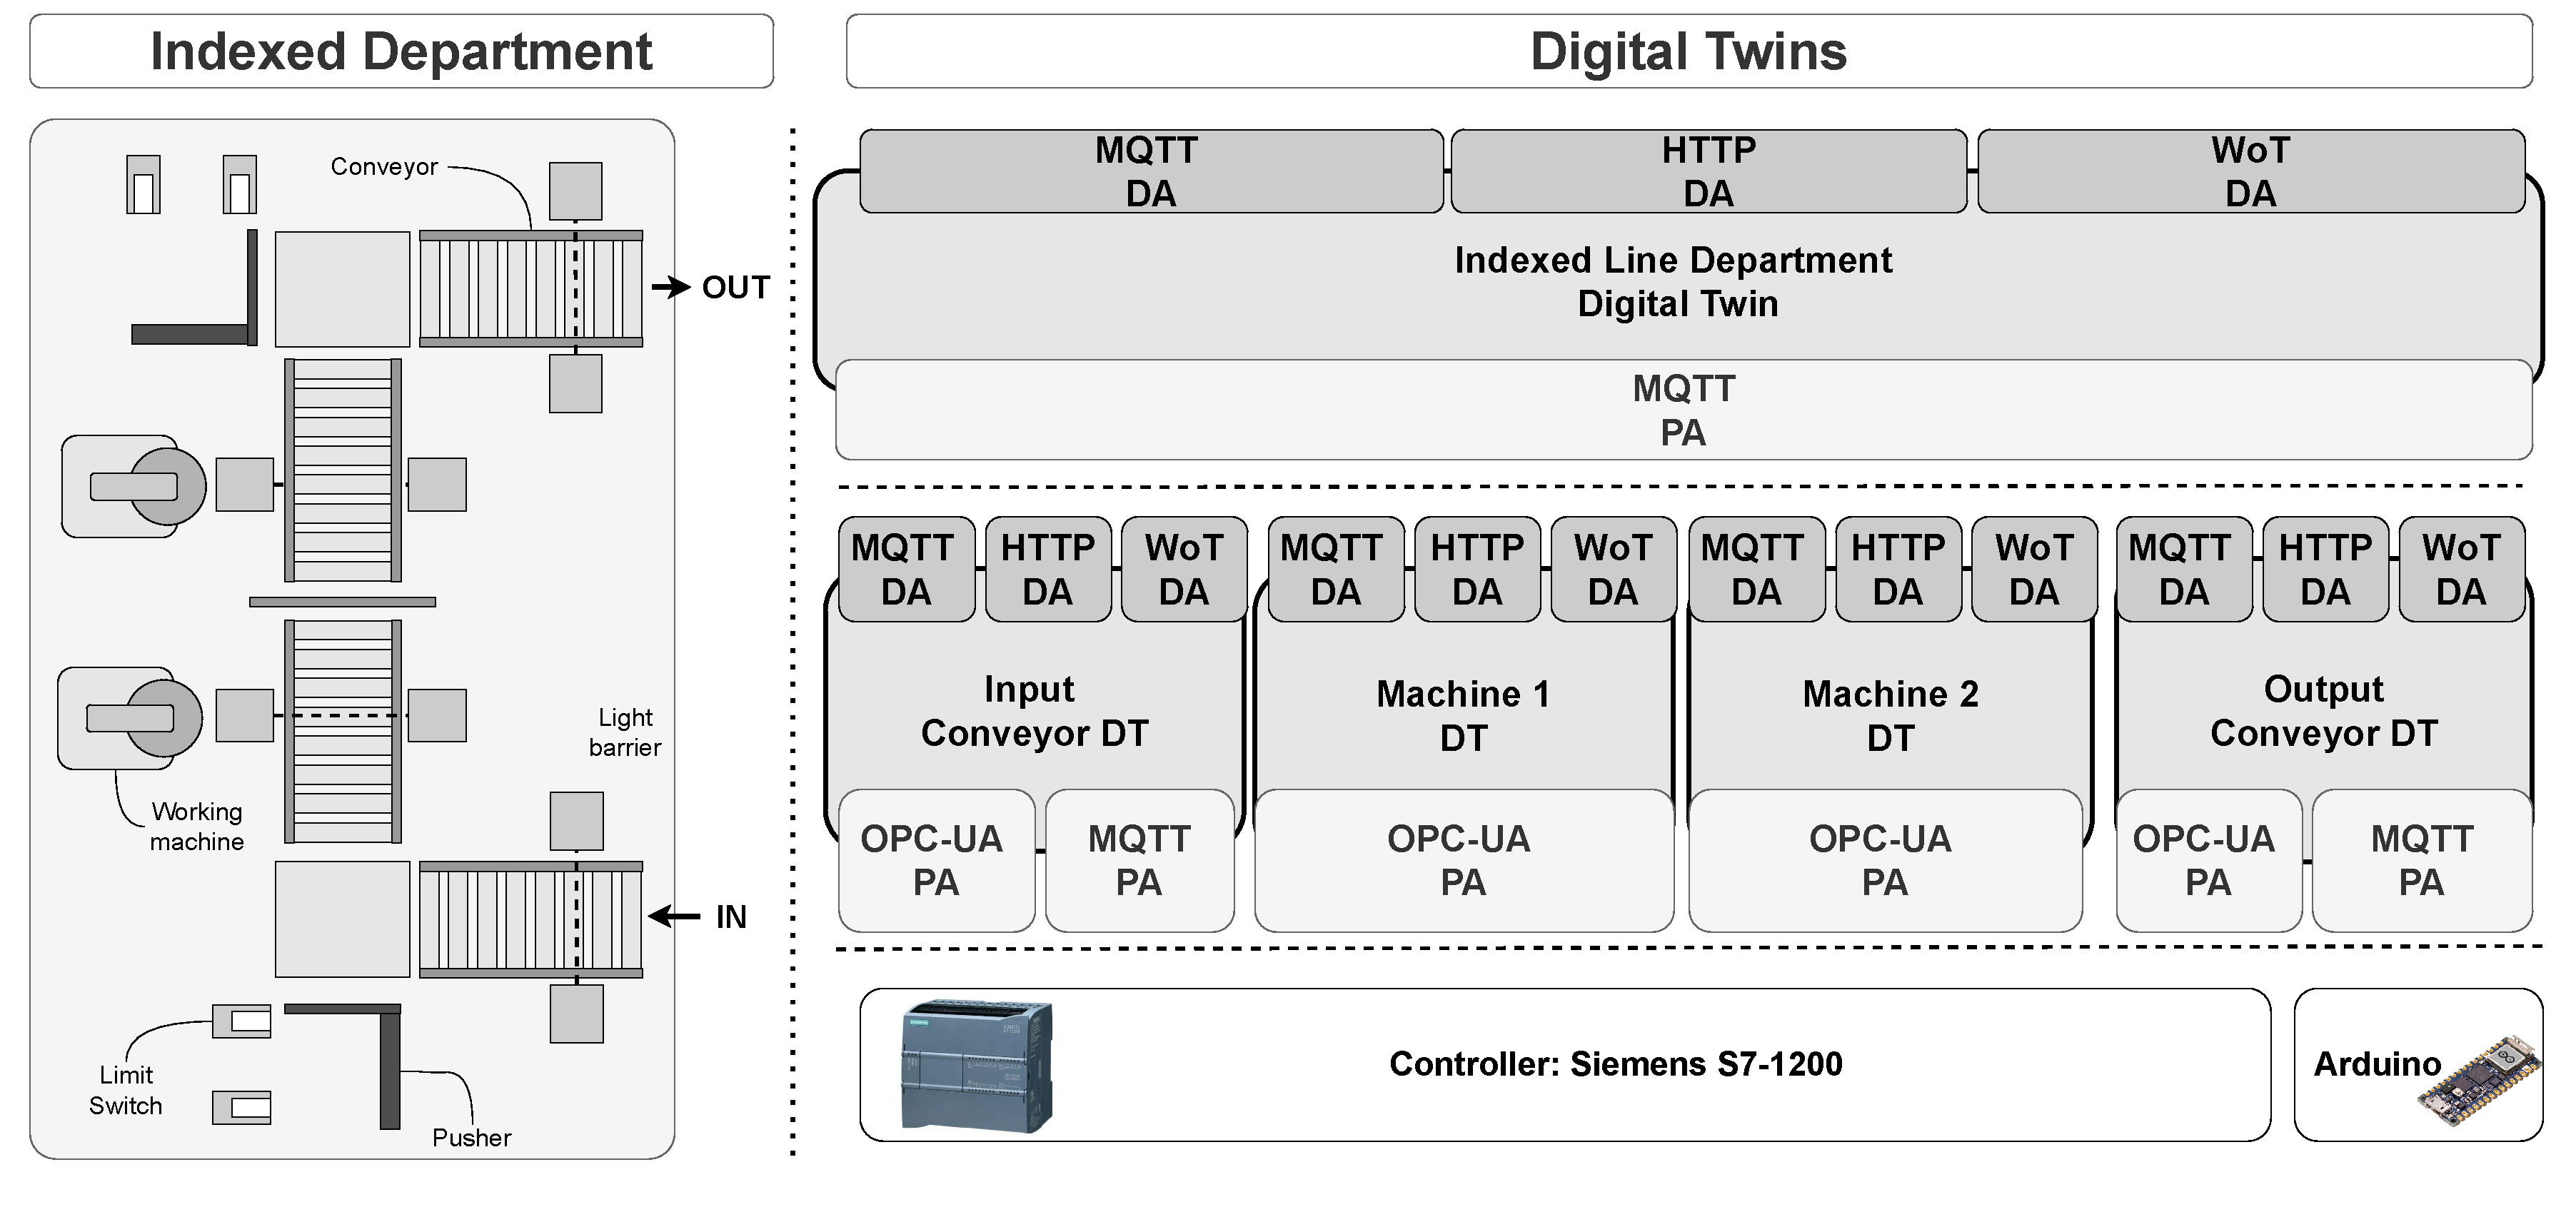
\includegraphics[width=0.93\linewidth]{figures/dt-interoperability/mf_dt_structure.pdf}
%     \caption{The \acl{DT} ecosystem architecture of the microfactory industrial system.}
%     \label{fig:mf_dt_ecosystem}
% \end{figure*}

%-------------------------------------------------------
\subsection{\acl{WoT}: enabling DT Interoperability}
\label{sec:dte:dt-engineering:wot-for-dt}
%-------------------------------------------------------

\ac{WoT}~\cite{wot-arch} standards (\Cref{chap:back:web:WoT}) share the goal of adopting uniform API and data format descriptions to hide low-level complexities and promote interoperability with the proposal of self-descriptive \ac{PhA} and \ac{DiA}.

Despite their similarities, \acp{PAD} and \acp{TD} serve distinct purposes. 
A \ac{TD} provides a structured description of a physical twin's available interactions to external consumers, detailing protocols and interaction possibilities.
%
In contrast, a \ac{PAD} is designed for internal use by the \ac{DT} modules, decoupling the twin's core from the complexities of communication channels.
Its primary role is to facilitate the discovery of available resources and capabilities on the \ac{PA} after establishing a connection with the physical counterpart, providing a structured description of its functionalities and data.
This description is directly interpretable by the \ac{DT} model and independent of the physical characteristics, allowing the reuse of the same model for similar \acp{PA} employing different communication channels.

In contexts in which \ac{WoT} standards are applicable, the devices' \acp{TD} can be automatically mapped to \acp{PAD}, streamlining the \ac{DT} creation process.
Leveraging \ac{WoT} \acp{TD} can significantly reduce the effort required to generate \acp{PAD}, particularly in environments where numerous physical twins already have associated \acp{TD}.
This convergence between \ac{WoT} and \ac{DT} architectures has the potential to accelerate the development and deployment of \ac{DT} solutions by promoting standardization and reusability.
%
Nevertheless, the more general concept of \ac{PAD} can be tailored also to those scenarios in which \ac{WoT} is not applicable. In those cases the responsibility falls back to development (or configuration) of a \ac{PhA} for a specific device to encode the necessary knowledge for the generation of the \ac{PAD}.

\ac{WoT} \acp{TD} can also be used as \acp{DTD}.
The \ac{WoT} architecture actually lists \acp{DT} as one of the possible deployment patterns, with a \ac{DT} mediating the interaction with a \ac{PA} behind a \ac{WoT} interface\footnote{\url{https://www.w3.org/TR/2023/REC-wot-architecture11-20231205/\#digital-twins}}.
%
This is especially useful when devices are not \ac{WoT} compatible or can not be made so due to other constraints, essentially retrofitting the capabilities of the devices with a \ac{WoT} compatible interface.
%
Adhering to \ac{REST} constraints~\cite{fielding2000architectural} and specifically to the HATEOAS and self-descriptive principles, a \ac{TD}-based \ac{DTD} facilitates the discovery of the \ac{DT} model and services.
%
Its machine-readable nature ensures interoperability for applications and consumers.
%
In particular, a \ac{TD}-based \ac{DTD} facilitates the inclusion of \acp{DT} in \ac{WoT} mashups, promoting \acp{DT} as valid \ac{WoT} Things usable by \ac{WoT} Consumers.

Despite its flexibility,
and broad applicability, 
using of \ac{TD} for \acp{DT} presents several limitations in capturing the specific characteristics of \acp{DT} that distinguish them from \emph{Things}.
%
A path to address these limitations could be extending \acp{TD} or supporting additional descriptions specifically for \acp{DT} in \acp{DTE} as explored in \Cref{chap:dte:hwodt}.



%=======================================================
\section{Managing the Digital Twin Lifecycle}
\label{sec:dte:engineering-dt:dt-lifecycle}
%=======================================================


Recently, there has been an increasing recognition of the importance of the lifecycle of \acp{DT},
particularly in distinguishing the properties that define the relationship between the \ac{DT} and \ac{PA}. 
%
Key concepts such as \emph{reflection} and \emph{entanglement} are critical for accurately representing the \ac{PA}~\cite{dt-IoT-context-Minerva-2020,web-of-dt-ricci-2022}.
%
These properties underscore the necessity for a structured lifecycle for the \ac{DT}, ensuring that its state remains consistently aligned with the \ac{PA} throughout various stages.
%
As highlighted in recent surveys~\cite{ferko2022architecting, 9640612,Hribernik_Cabri_Mandreoli_Mentzas_2021}, while the body of literature on \ac{DT} software architectures is growing, most papers are domain-specific and focus on reference models.
%
However, these models often lack concrete guidance on how to implement the internal components of a \ac{DT}. Many of the existing models envision multiple parallel components or models working together, but fail to address how they communicate and interact to maintain consistency in the \ac{DT} state.
This gap leads to potential inconsistencies between the \ac{DT} and \ac{PA}, as the interaction between models and the management of state changes is not adequately captured~\cite{alam2017access,Malakuti2019fourlayer,Lpez2021}.




\begin{figure}[t]
    \centering
    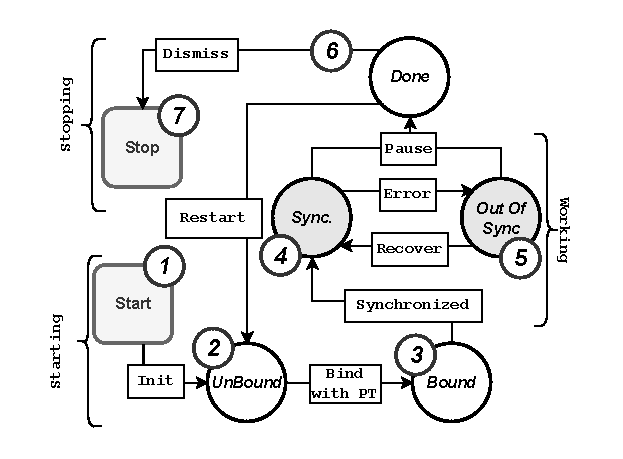
\includegraphics[width=\columnwidth]{figures/wldt_lifecycle_simple.pdf}
    \caption{DT Life Cycle with its phases and transitions.}
    \label{fig:dt_life_cycle}
\end{figure}


%START FROM HERE

%-------------------------------------------------------
\subsection{A Digital Twin Synchronization Lifecycle}
%-------------------------------------------------------

The concept of a \ac{DT} lifecycle has recently been introduced and examined, focusing on its core components and the integration of both the software nature of the \ac{DT} and its ability to synchronize with the \ac{PA} over time~\cite{web-of-dt-ricci-2022}.
%
This lifecycle encompasses the various phases that a \ac{DT} undergoes, as shown in Figure~\ref{fig:dt_life_cycle}, from its creation to deactivation.
%
Since a \ac{DT} is fundamentally a software entity, it is vital to track the evolution of such phases considering the different stages of synchronization with its \ac{PA}.
Proper observation and modeling of this lifecycle are essential to ensure that the \ac{DT} representation can be trusted to reflect the physical counterpart's state consistently when the \ac{DT} is \texttt{Synchronized} and can instead be considered to be outdated in the other phases.

The execution lifecycle of a \ac{DT} can be modeled as follows.
Upon creation (from the \texttt{Started} phase),
the \ac{DT} enters the \texttt{Unbound} phase, where all internal modules are initialized and prepared for the binding process with the \ac{PA}.
%
Once the \ac{DT} successfully binds to its \ac{PA},
meaning the \ac{PA} meets the necessary requirements (expected functionalities and properties)
and the \ac{DT} can communicate with it,
the \ac{DT} enters the \texttt{Bound} phase.
%
During this phase, the \ac{DT} is connected to the \ac{PA} and is ready to begin the shadowing process.

The next phase is the \texttt{Synchronized} phase, 
this is different from simply having established a connection with the \ac{PA}, 
but rather indicates that the \ac{DT} is complying with application-specific requirements
and is receiving the necessary and correct amount of information to be fully aligned with its \ac{PA}.
%
During the synchronization phase the \ac{DT} can compute the \ac{DT} state ($S_{DT}$), ensuring that it is able to accurately reflects the status of its physical counterpart.

If any issues arise, such as network failures, and the \ac{DT} synchronization performance falls under the expected requirements, the \ac{DT} enters the \texttt{Out of Sync} phase.
In this state, the \ac{DT}---while still operational---is unable to update its state reliably. 
%
Eventually, the \ac{DT} may return to the \texttt{Synchronized} phase.

Finally, when the \ac{DT} is no longer required or has completed its function, it transitions to the \texttt{Done} phase.
In this phase, the \ac{DT} remains accessible to external consumers and retains its memory, but it is no longer bound to the \ac{PA} or in sync with it. At the end of the lifecycle, the \ac{DT} can be dismissed and moved to the \texttt{Stopped} phase.
Throughout its lifecycle, the \ac{DT} may also return to the \texttt{Unbound} phase if errors are detected during the binding process or if it is rebooted or restarted.


%-------------------------------------------------------
\subsection{Binding the DT with the PA}
%-------------------------------------------------------

The transition from the Unbound to Bound phase in the \ac{DT} lifecycle remains an open research area:
a key challenge is identifying whether all the capabilities of the \ac{PA} relevant to support the \ac{DT}'s behavior are available so that the shadowing process can start.

The modular design of the \ac{PI} presented in the previous section (\Cref{ssec:dte:dt-engineering:physical_interoperability}) can have support this transition.
%
Namely, once a \ac{PhA} successfully connects to the \ac{PA}'s channel and starts receiving data from it, it can send the generated \ac{PAD} to the \ac{DT} model.
The generation of the \ac{PAD} can be used as a synchronization step to signify that the \ac{PhA} is successfully connected to the \ac{PA}.
%
The \ac{DT} model is then responsible for collecting the different \acp{PAD}, assessing whether all the relevant information to start computing the \ac{DT} state is available and consequently moving on to the \texttt{Bound} phase.
%
This mechanism enables managing the \ac{DT} behavior consistently, even with the additional complexity of the modular \ac{PI} design.

Of course the challenge still stands in managing each individual \ac{PhA} connection, but this decoupling through \acp{PAD} allows \ac{DT} developers to establish functional binding requirements that are independent of technical details. 

%--------------------------------------------------------
\subsection{Managing DT and PA Synchronization}
%--------------------------------------------------------


The most significant challenge in current \ac{DT} lifecycle modeling is the broad characterization of the \texttt{Synchronized} phase, which
only generically considers synchronization requirements between the \ac{PA} and the \ac{DT}, without having explicit awareness of the \ac{PA} lifecycle and the potential changes in its operational context.
This general and unstructured approach limits the ability to model the lifecycle in a consistent and uniform manner, failing to properly address the dynamism of the \ac{PA} behavior.

The \texttt{Synchronized} phase of the \ac{DT}'s lifecycle assumes a continuous exchange of information between the \ac{DT} and its associated \ac{PA} usually measured to maintain a frequency within a given threshold, to guarantee that information on the \ac{DT} is \emph{fresh} and can hence be trusted as a valid representation of the \ac{PA} state. 

However, this general assumption may not always hold true due to variations in the \ac{PA}'s internal states.
% The issue arises because \ac{PA} can adjust telemetry frequency and have different value ranges over time, depending on the phases of their lifecycle and their operational context (e.g., from \texttt{Ready} to \texttt{Working}).
% These variations introduce complexity in maintaining the cyber-physical alignment. 
% Without appropriate modeling, these changes might be misinterpreted as failures while they are instead expected variations due to the \ac{PA}'s phase transition.
%
In some cases, \acp{PA} can enter operational states that temporarily inhibit their ability to communicate, even while maintaining an active connection to the \ac{DT}.
These are scenarios in which the absence of messages from the \ac{PA} does not necessarily indicate a failure or misalignment but rather reflects the \ac{PA}'s operational context.
For instance, a \ac{PA} might enter a \texttt{Rebooting} state during which it cannot send telemetry data.
Similarly, resource constraints on the \ac{PA}, such as \textit{CPU overload} or \textit{network bandwidth exhaustion}, may result in disrupted or paused communication that may or may not be tolerable for the \ac{DT} model and application.
%
In other cases, the \ac{PA} may not entirely cease communication but instead alter its update frequency in response to operational changes. For example, an industrial robotic arm might increase its data transmission frequency during a high-precision assembly task to provide real-time feedback, while it could reduce the update rate to conserve energy and network bandwidth when in an idle or maintenance mode.


\begin{figure}
    \centering
    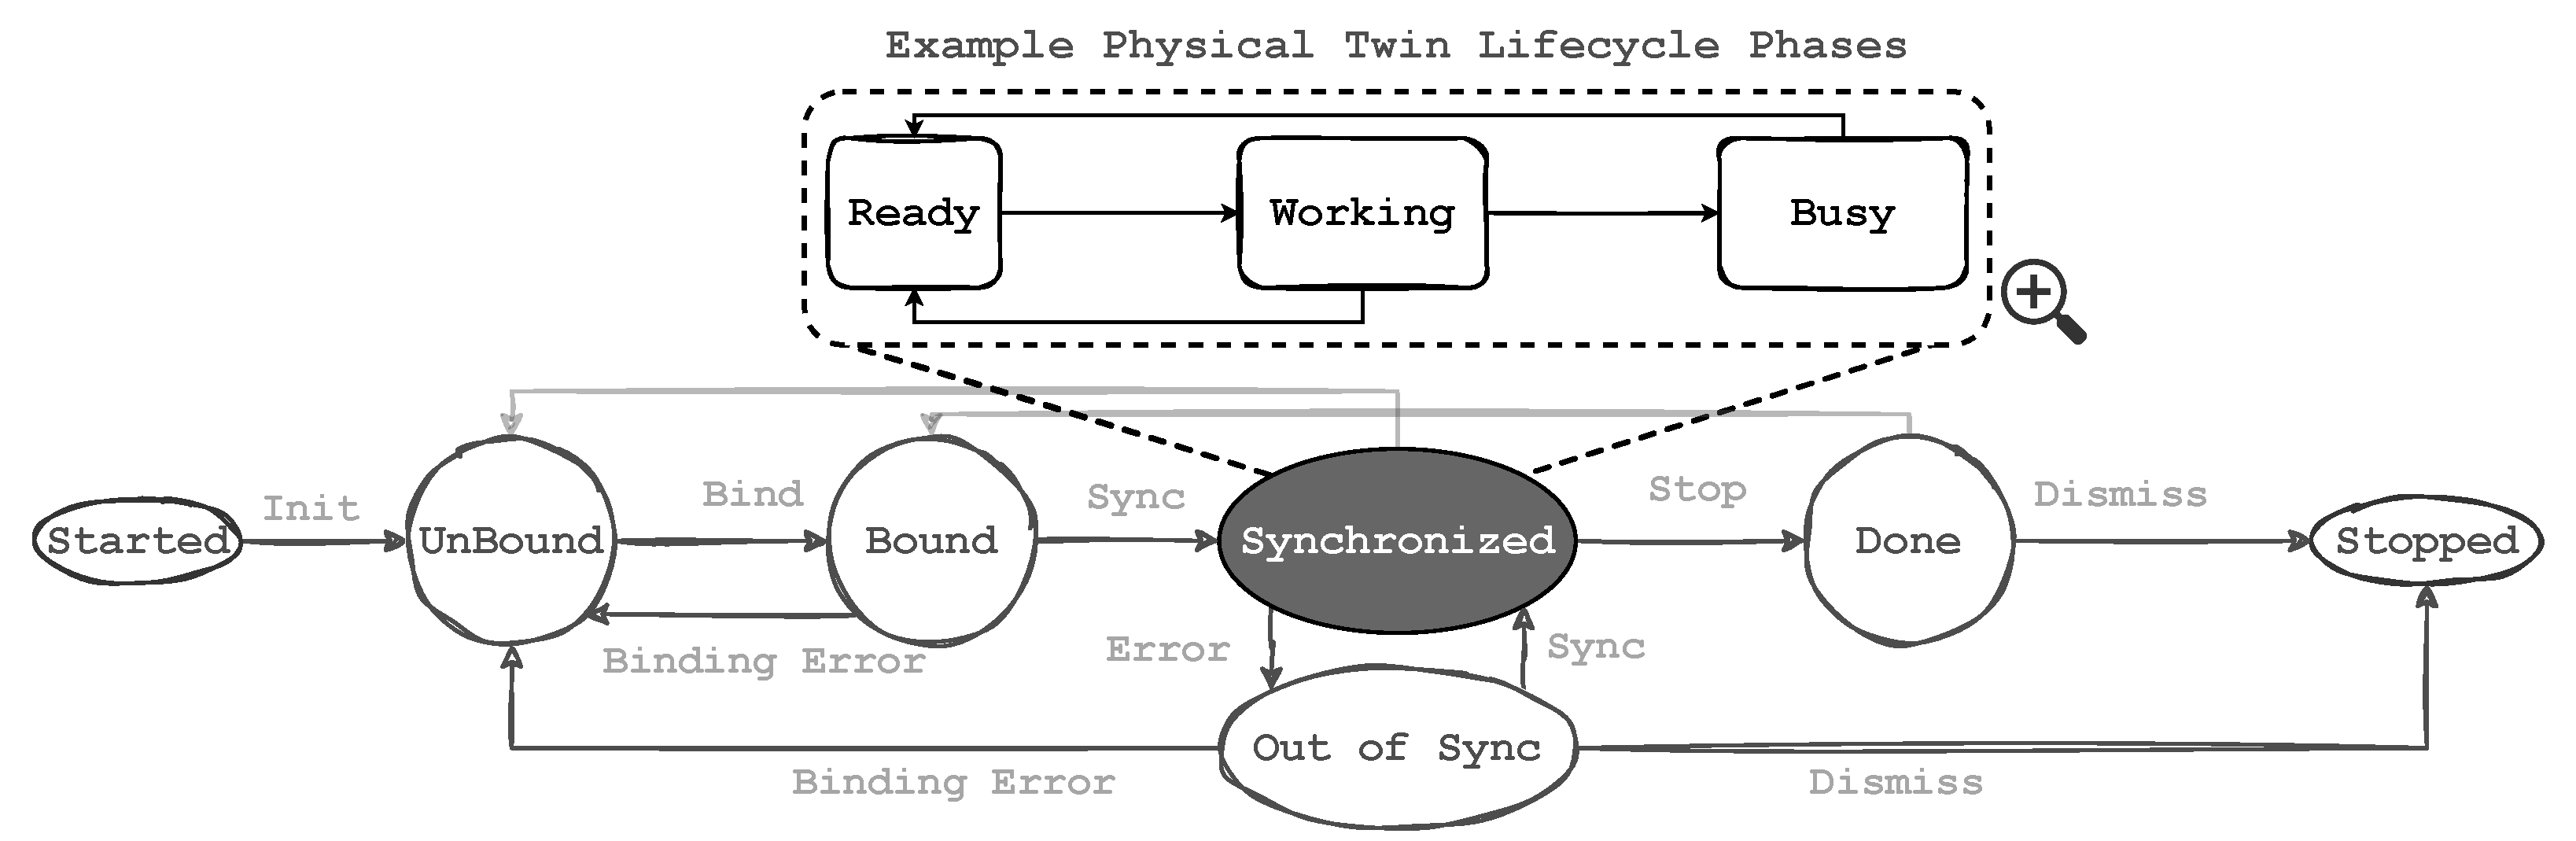
\includegraphics[width=\textwidth]{figures/dt-lifecycle/dt_lifecycle_pt_sync.pdf}
    \caption{Schematic representation of the \ac{DT} lifecycle with a structured example of the Synchronized phase.}
    \label{fig:dt_lifecycle_pt_sync}
\end{figure}


This adaptive behavior necessitates that the \ac{DT} \emph{dynamically adjust its expectations} and processing strategies based on the \ac{PA}'s operational state, avoiding false-positive anomalies caused by \emph{intentional} communication variability.  
By distinguishing between inhibited communication (e.g., \texttt{Rebooting} or \texttt{Overloaded}) and adjusted communication patterns (e.g., frequency scaling in \texttt{Idle} vs. \texttt{Active} states), the \ac{DT} can better align with the \ac{PA}'s lifecycle.
This alignment ensures the \ac{DT} remains a reliable digital counterpart, accurately reflecting the \ac{PA}'s operational context and providing a robust foundation for decision-making.  

To address these situations, the \ac{DT} must incorporate mechanisms to: 
\begin{itemize}
    \item \emph{Detect and Classify Non-Communication States:} Recognize when the lack of communication from the \ac{PA} is due to a valid operational state (e.g., rebooting) rather than a system failure;
    \item \emph{Model \ac{PA} State-Dependent Communication Behavior:} Explicitly account for \ac{PA} states that imply non-communication, such as \textit{idle}, \textit{rebooting}, or \textit{overloaded}, within the lifecycle framework. 
\end{itemize}
This requires extending the \ac{DT} lifecycle model (\Cref{fig:dt_life_cycle}) to represent such scenarios accurately.


The proposal is to refine the \texttt{Synchronized} phase by introducing sub-phases that correspond to the \ac{PA}'s operational states (\Cref{fig:dt_lifecycle_pt_sync}).
For example, in the industrial domain, a \ac{DT} of a machine may enter the \texttt{Synchronized} phase but should then transition through more specific sub-phases such as \texttt{Ready}, \texttt{Working}, or \texttt{Busy}.
Each of these sub-phases would have clearly defined transition criteria, phases, and associated $S_{\ac{DT}}$, providing a more granular and accurate representation of the \ac{DT}'s behavior.

To formalize this approach, the overall \ac{DT} lifecycle phase at a given time $t$ $LP_{DT}(t)$ can be defined as a composition of the \ac{PA} lifecycle phase $LP_{PA}(t)$ and the \ac{DT} software lifecycle phase $LP_{Soft.}(t)$, as shown in Eq.~\ref{eq:lpdt_definition}.

\begin{equation}
LP_{DT}(t) = \langle  LP_{PA}(t), LP_{Soft.}(t)\rangle
\label{eq:lpdt_definition}
\end{equation}

The \ac{DT} representation of the asset $R_{DT}$ can hence be characterized at any given time instant $t_i$ by its lifecycle phase $LP_{DT}(t_i)$, its current state $S_{DT}(t_i)$, and its history $H(t_a, t_b)$ over a specific time interval $(t_a, t_b)$, as shown in Eq.~\ref{eq:dt-definition}.

\begin{equation}
R_{DT}(t_i) = \langle LP_{DT}(t_i), S_{DT}(t_i), H(t_a, t_b)\rangle \quad \text{and} \quad  t_a, t_b \leq t_i
\label{eq:dt-definition}
\end{equation}

The values of the different components of the \ac{DT} at the time instant $t_i$ can then be mapped as a function of the different possible values of $LP_{Soft.}$, as detailed in Eq.~\ref{eq:lpdt_complete_mapping}.

\begin{equation}
\begin{split}
R_{DT}(t_i) = {} &
\begin{cases}
    LP_{PA} = \emptyset, \ S_{DT} = \emptyset, \ H = \emptyset,\\
    \quad \text{if } LP_{Soft.} \in \{\texttt{Started}, \texttt{Stopped}\}, \\[0.4em]
    LP_{PA} = \emptyset, \ S_{DT} = \emptyset, \ H = H(t_f, t_o),\\
    \quad \text{if } LP_{Soft.} \in \{\texttt{UnBound}, \texttt{Bound}, \texttt{OutOfSync}\}, \\[0.4em]
    LP_{PA} = LP_{PA}(t_i), \ S_{DT} = S_{DT}(t_i), \ H = H(t_f, t_i),\\
    \quad \text{if } LP_{Soft.} = \texttt{Synchronized},\\[0.4em]
    LP_{PA} = \emptyset, \ S_{DT} = \emptyset, \ H = H(t_f, t_d),\\
    \quad \text{if } LP_{Soft.} = \texttt{Done}
\end{cases}
\end{split}
\label{eq:lpdt_complete_mapping}
\end{equation}

When $LP_{Soft.}$ is \texttt{Started}, it represents the initialization phase where the \ac{DT} software has been instantiated. At this stage, $LP_{PA}$ is undefined since no communication with the \ac{PA} has been established. 
Similarly, $S_{DT}$ has not been computed, as the \ac{DT} has not acquired any state information. The history $H$ is also empty, as no synchronization or state updates have occurred yet.

When $LP_{Soft.}$ is \texttt{Unbound}, it indicates that the \ac{DT} is operational but not yet synchronized.
In this phase, $LP_{PA}$ remains undefined because the \ac{PA} lifecycle phase cannot be detected.
$S_{\ac{DT}}$ is also undefined since the \ac{DT} can not compute the state yet.
However, the history $H$ retains information about events recorded from the first connection data received from the \ac{PA} $t_{f}$ to the moment the \ac{DT} transitioned out of the synchronized phase, marked by $t_{o}$.
%
The same happens when the \ac{DT} is \texttt{Bound}, as the state has not been computed yet, 
or if the \ac{DT} is \texttt{Out of Sync}, as the state can no longer be updated.

When $LP_{Soft.}$  is \texttt{Synchronized}, the \ac{DT} is fully synchronized with the \ac{PA}.
In this state, $LP_{PA}$ corresponds to the lifecycle phase of the PA (e.g., in the example of Fig.~\ref{fig:dt_lifecycle_pt_sync}, this could be the \texttt{Working} phase) at the time $t_i$.
At this point, $S_{DT}$ contains the current computed state of the \ac{DT}, reflecting the alignment between the \ac{DT} and \ac{PA}.
The history $H$ encompasses all events and states up to the current time $t_{i}$, documenting the \ac{DT}'s evolution in sync with the PA.
If the \ac{DT} operates correctly, it can remain in the \textit{Synchronized} phase for the duration of its lifecycle, continually updating as the PA's lifecycle progresses.
During this phase, multiple records of lifecycle evolution can be captured as $LP_{PA}$ evolves (e.g., moving from \texttt{Working} to \texttt{Busy}), and multiple computations of $S_{DT}$ may occur within the same $LP_{PA}$.
For instance, while in the \texttt{Working} phase, the \ac{DT} could compute multiple states corresponding to variations in physical properties such as accelerometer readings or energy consumption, ensuring the \ac{DT} continuously reflects the PA's behavior in a dynamic and precise manner.

When $LP_{Soft.}$ is \texttt{Done}, the \ac{DT} synchronization has been intentionally paused, and the \ac{DT} remains active for accessing stored information. In this phase, $\text{LP}_{PA}$ is empty, $S_{DT}$ is empty, and $H$ contains the history until the time the \ac{DT} is decommissioned denoted as $t_{d}$.

Finally, when $LP_{Soft.}$ is \texttt{Stopped}, the \ac{DT} lifecycle is terminated. $LP_{PA}$ is empty, $S_{DT}$ is empty, and $H$ is also empty, as the \ac{DT} is offline and data is no longer accessible.

By clearly defining and distinguishing between the various phases, the approach enhances the alignment between \ac{DT}s and their physical counterparts, ensuring that each transition and state change is accurately captured and reflected.
The main benefits of this approach include: 
\begin{itemize}
    \item \textit{Enhanced Cyber-Physical Awareness}: a structured lifecycle model ensures that critical transitions of phases and states of the \ac{PA} are precisely tracked and understood, enhancing the overall awareness and responsiveness of the system;
    \item \textit{Better Decision-Making}: with a clear understanding of each phase and its impact, applications and services can make more informed decisions based on accurate and timely information about the current relationship between \ac{PA} and \ac{DT};
    \item \textit{Adaptability}: this structured approach can be adapted to various applications, making it versatile and applicable across different domains.
\end{itemize}

The approach assumes that the $L_{PA}$ is either provided by the \ac{PA} or can be identified by the \ac{DT} model (e.g., through a classification model).
Modeling these phases can be challenging, especially for complex \acp{DT}.
Despite improved cyber-physical awareness, phases may still be incorrectly mapped due to unforeseen external factors.
Additionally, phase tolerance could impact anomaly detection within the DT, necessitating methodological trade-offs to set this tolerance correctly.

Despite these open challenges, the proposed structured lifecycle model represents an advancement in managing \ac{DT} synchronization with their physical counterparts, providing a robust foundation for future developments.

%=======================================================
\section{Modeling Augmentation Functionalities}
\label{sec:dte:engineering-dt:dt-augmentation}
%=======================================================

\acp{PA} are typically limited by the nature of their physical characteristics throughout their lifecycle. In contrast, \acp{DT} can capitalize on software-based flexibility to modify, update, and enhance functionality over time.
These enhancements are accessible through \ac{DT} \acp{API} and can be powered by data-driven models possibly enabling adaptive and intelligent behaviors.
This core property of \acp{DT} is known as \emph{augmentation}~\cite{dt-IoT-context-Minerva-2020}.

Examples of DT-enabled augmentation include adding technical features to retrofit devices through external software, such as enhancing interoperability of \ac{IoT} devices via protocol and data format translation. Another example involves improving security and addressing unresolved bugs by mediating interactions with outdated devices that no longer receive updates. Additionally, \acp{DT} can enhance device services by introducing new high-level actions for operations, or by implementing advanced functionalities powered by machine learning and \ac{AI} algorithms, such as forecasting, anomaly detection, and pattern recognition (\Cref{sec:back:dt:ai}).

Despite the acknowledgment of augmentation as a defining feature of \acp{DT},
this property is often defined only conceptually, with implementations tailored to specific vertical cases.
The lack of a reference model for defining \ac{DT} augmentation results in unclear design patterns and potential performance limitations.
Indeed, without a well-defined and measurable boundary for augmentation features---including resource allocation---the \ac{DT} risks failing to achieve its design goal of accurately representing the \ac{PA} with sufficient \emph{fidelity}~\cite{Bellavista_Bicocchi_Fogli_Giannelli_Mamei_Picone_2023}.

%--------------------------------------------
\subsection{Extending the DT Model with Augmentation}
%--------------------------------------------

The \ac{DT} model introduced in \Cref{sec:dte:engineering-dt:abstract-architecture} is here extended to explicitly include augmentation functionalities.
%
In practical terms, augmentation serves as a bridge transforming raw data into meaningful, actionable outcomes guided by the underlying model.
\acp{DT} may expose additional services and functionalities that enhance the capabilities of the \ac{PA}.
Such functionalities can be represented as a set of \emph{augmentation functions} $F$, where $Augm_{i}$ denotes the individual augmentation functions implemented within the DT. Each augmentation function $Augm_i$ may leverage a specific model $m \in M$, to interpret and respond to changes in the DT.

\begin{equation}\label{eq:augm_set}
    F = \{Augm_{1}, Augm_{2}, \dots, Augm_{n}\}\\
\end{equation}

The model in \Cref{eq:5D_dt_model} can hence be extended to: 

\begin{equation}
DT = \langle PI, M, Shad, F, H, DI \rangle
\tag{\ref{eq:5D_dt_model}}
\end{equation}

Augmentation functions can be distinguished based on two aspects:


\paragraph{Triggering mechanism} (\( \tau \)): defines how and when the function is activated in response to events within the \ac{DT}.
%
\begin{equation}
\tau \in \{ e_{DT}, e_{Aug}, e_{Time} \}  \sigma \in \{S_{aug}, \varnothing\}
\end{equation}
%
\(\tau\) can be an event of three types:
%
\begin{itemize}
\item \( e_{DT} \) represents the output from the shadowing process indicating a new computation of the \ac{DT} state \( S_{DT} \);
\item \( e_{Aug} \) can be generated either as the output of another augmentation function or as a direct invocation by the shadowing process;
\item \( e_{Time} \) refers to temporal triggers and can be used to model periodic execution or specific scheduled tasks.
\end{itemize}
%
Notably, augmentation functions can not respond to triggers coming directly from the \ac{PI} as such $e_{PA}$.
Physical events need to be processed by the shadowing process first, which may in turn select the activation of a relevant augmentation function firing a specific $e_{Aug}$.



\paragraph{State management} (\( \sigma \)): indicates whether the function maintains an internal state that persists over time or is \emph{stateless}.
%
\begin{equation}
\sigma \in \{S_{aug}, \varnothing\}
\end{equation}
%
A stateful function possesses a state \( S_{Aug} \) that evolves and persists over time in alignment with the evolution of the \ac{DT}.  
A stateless function simply reacts to triggers without maintaining any memory of previous invocations.  
Notably, modeling stateful functions allows for the representation of processes that may even run in parallel with the \ac{DT} main control flow, producing new events \( e_{Aug} \) asynchronously.  
Since the function is stateful, it is triggered to start but can persist over time, as its execution is fully encapsulated within the function context. Additionally, the function may receive new triggers over time that feed into its ongoing process.

The output of an augmentation function \( Augm_{i} \) is determined by its inputs and can be expressed as:

\begin{equation}
    Augm_{i}(\tau, m, \sigma, H) =
    \begin{cases}
    e_{Aug} & \text{\textbf{if} $m$ matches}\\
    \varnothing & \text{\textbf{otherwise}}
    \end{cases}
\end{equation}

The triggering event $\tau$ may carry important information for the function execution.
The parameter $m \in M$ represents the model used within the augmentation function, encapsulating the rules, logic, and conditions that define how the function interprets its inputs and determines the output.
The model is crucial for evaluating whether the function should generate an output based on the current state of the function $\sigma$ and context, which is represented by the \ac{DT} history $H$ which includes the latest state $S_{DT}$.

The output \( e_{Aug} \) represents an event generated by the augmentation function, signaling that the conditions defined by the model \( m \) have been met. Conversely, if the conditions are not satisfied (i.e., if \( m \) does not align with the current state or inputs), the output will be \( \varnothing \), indicating that no new event has been produced.  
This approach captures the idea that the execution of an augmentation function does not always result in the generation of a new event. For example, in the case of an anomaly detection model, an event is only triggered when an anomaly is detected with a certain confidence threshold, meaning that no event is generated if the conditions for an anomaly are not met.
Since $e_{Aug} \in \tau$, augmentation functions can also be chained to model processing pipelines triggered by the outputs of previous functions.

%--------------------------------------------
\subsection{Impact on Shadowing}
%--------------------------------------------

The introduction of augmentation functions requires to adapt the shadowing process to handle augmentation events. Indeed, the shadowing process should be capable of receiving relevant augmentation events (e.g., detected anomalies) and use them to update the state of the DT, as illustrated below:

\begin{equation}
    e_{DT}(S_{DT}) = Shad_{DT \rightarrow DT}(M, e_{Aug}, H)
\end{equation}

The same principle applies when a physical event triggers an augmentation function. There is no direct link between physical world events (\( e_{PA} \)) and augmentation functions; 
instead, the decision to trigger an augmentation function based on the receipt of a physical event is mediated by the shadowing process.
The shadowing process analyzes the \( e_{PA} \) and determines whether it is relevant for an augmentation function in $F$ (or multiple functions simultaneously).  If the event is deemed as relevant, the shadowing process generates a trigger by producing an augmentation event (\( e_{Aug} \)), which then serves as the trigger \( \tau \) for one or more augmentation functions.

\begin{equation}
    e_{Aug} = Shad_{PA \rightarrow DT}(M, e_{PA}, H, F)
\end{equation}


Similarly, actions requests that are received by the \ac{DT} ($a_{DT}$) can also trigger augmentation functions.
Again, there is no direct relationship between the action taken on the DT, as represented by its state, and the execution of the augmentation function. Instead, this process also goes through the shadowing process, which matches the request received on the \ac{DI} with the corresponding augmentation function trigger, thus generating an augmentation event that will serve as the trigger for the augmentation function.
This can be used to model a request-response pattern for the execution of augmentation functions such as requesting the predicted next state of the \ac{DT}. In such cases, since the result of the augmentation does not impact the state of the \ac{DT}, the result can be directly routed to the external consumer of the \ac{DT}.

\begin{equation}
    e_{Aug} = Shad_{DT \rightarrow DT}(M, a_{DT}, H, F)
\end{equation}


Despite the shadowing might not be required to validate the result of an augmentation function triggered by an action request, it is still enforced to handle the incoming requests. 
This design aims to decouple the available implementations of the augmentation functions from the actions presented on \ac{DI} and handle this transparently from the consumer perspective.
For example, there might be several augmentation functions implementing a given functionality and it would be up to the shadowing process to determine which one is best suited to respond to a specific request depending on the current context of the \ac{DT} (e.g. the state prediction functionality could be implemented using different specialized models depending on some conditions in the state of the \ac{DT}).

%----------------------------------------------
\subsection{Engineering Augmentation Functions}
%----------------------------------------------

Engineering augmentation functions following the proposed model requires defining
software architectural patterns that can be practically applied to implement them.
Depending on the implementation, it is possible to define \emph{internal} and \emph{external} augmentation.  
This setup allows for the dynamic addition of new functionalities to the \ac{DT}, either through external or internal processing.

\begin{figure}
    \centering
    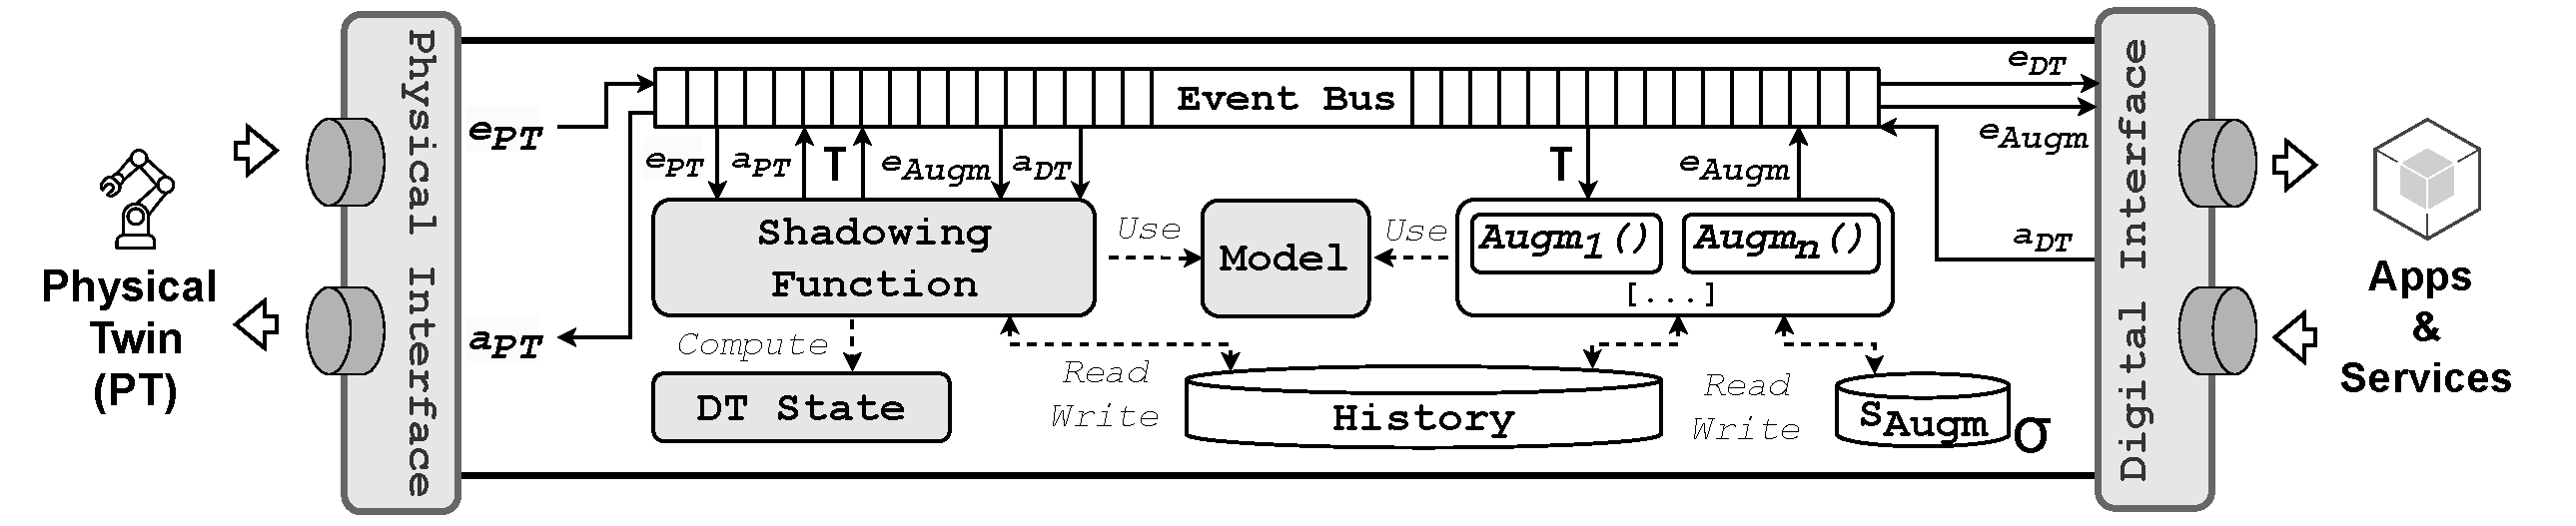
\includegraphics[width=\textwidth]{figures/event_driven_augmentation.pdf}
    \caption{Event-Driven architecture of a DT to support and enable effective Augmentation function management and execution.}
    \label{fig:event_driven_augmentation}
\end{figure}

As \Cref{fig:event_driven_augmentation} shows, the core architecture of the \ac{DT} is centered around a shared \texttt{Event Bus}, which serves as the communication backbone, handling events and actions within the \ac{DT} system.
Starting from the \ac{PI}, physical events \( e_{PA} \) are processed by the \texttt{Shadowing Function} ($Shad$) which computes the \ac{DT} State $S_{DT}$ based on the received events and the \texttt{\ac{DT} Models} ($M$), ensuring that the \ac{DT} accurately reflects the current state of the \ac{PA}.
The \texttt{\ac{DT} State} component maintains this state in memory, while the \texttt{History} ($H$) component persists past events and states for reference and analysis.

\texttt{Augmentation Functions} (\( Augm_{i} \)) provide additional capabilities or insights to the \ac{DT}, interacting with \( M \), \( H \), and internal state information \( \sigma \).
The interaction between the \( Shad \) and the \( Augm_{i} \) is entirely event-driven, based on trigger events \( \tau \) and \( e_{Augm} \) flowing out of the augmentation functions with their results.
These results are then sent to the \( Shad \) for further state computation and to the \texttt{Digital Interface} (\( DI \)) to respond to requests for \( Augm_{i} \) from external services and applications.
The \( DI \), mirroring the \ac{PI}, handles outgoing events of the \ac{DT} (e.g., \( e_{DT} \) carrying the new \( S_{DT} \) or its variations) or \( e_{Augm} \) with the results of an augmentation function, and manages incoming actions and requests from digital entities as digital actions \( a_{DT} \).

\begin{figure}
    \centering
    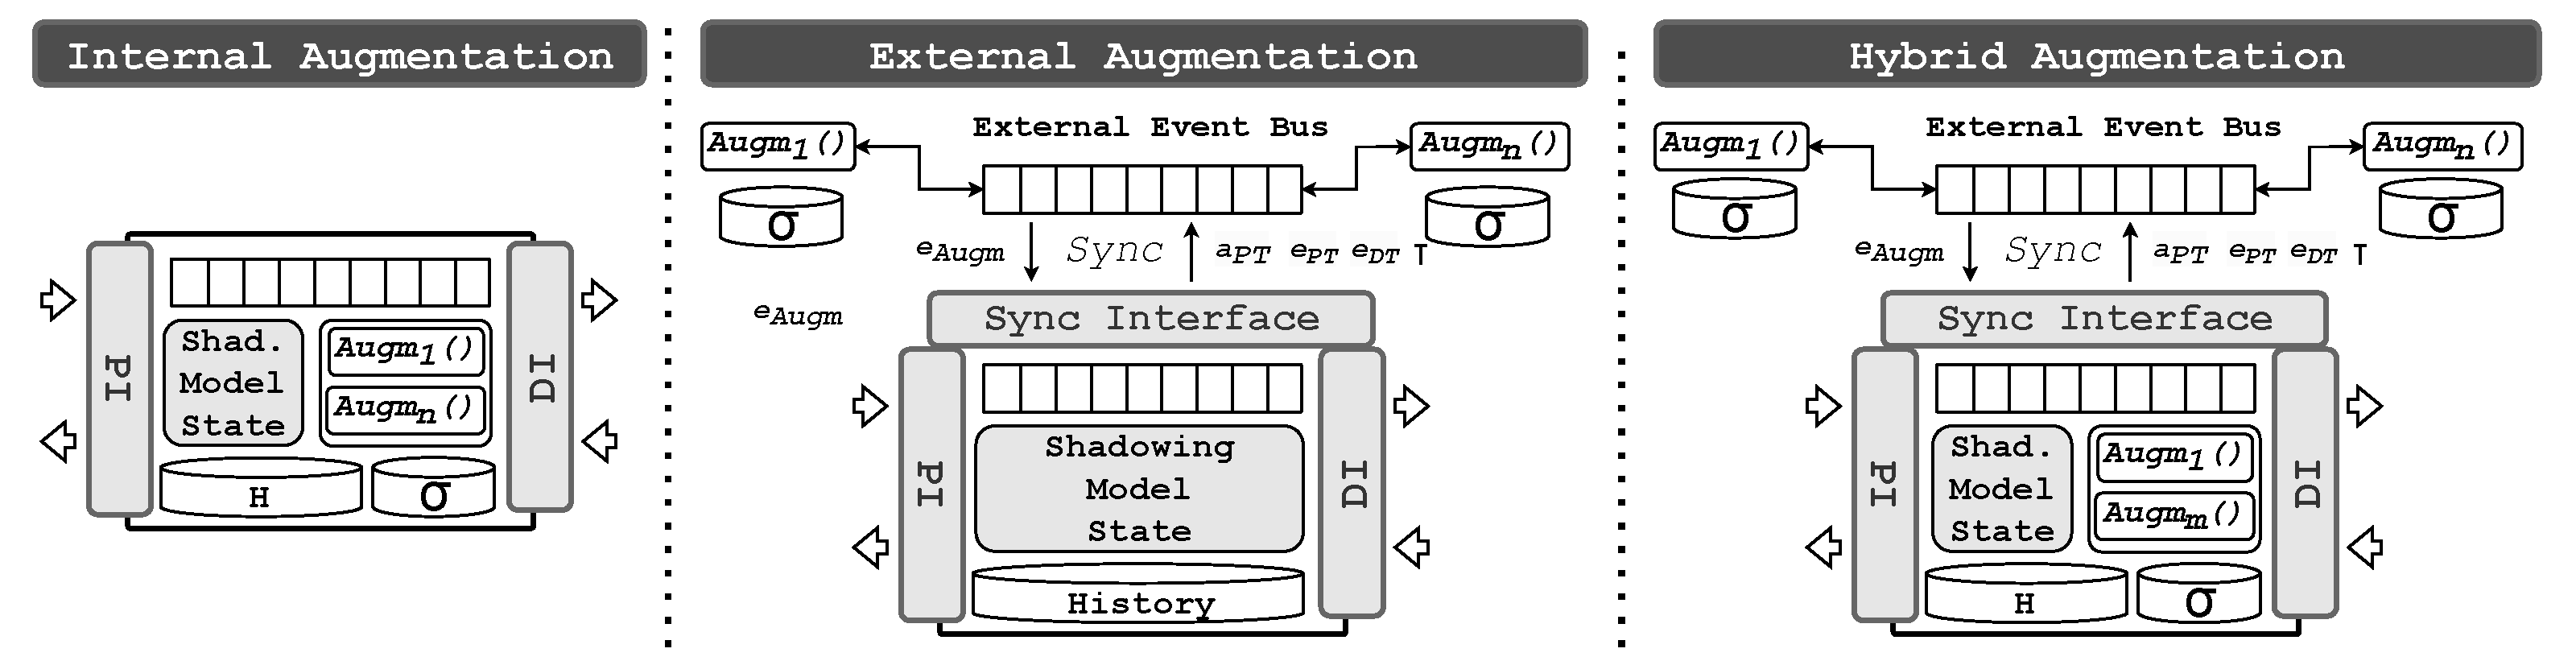
\includegraphics[width=\textwidth]{figures/augmentation_patterns.pdf}
    \caption{Patterns for augmentation functions execution: internally (left), externally (center), or through a hybrid solution (right).}
    \label{fig:augm_function_event_driven_patterns}
\end{figure}


Based on this event-driven model, it is possible to identify three approaches for implementing augmentation functions (\Cref{fig:augm_function_event_driven_patterns}):
\begin{itemize}
    \item \textit{internal} augmentation, where functions are executed within the \ac{DT} process;
    \item \textit{external} augmentation, where functions are executed outside the \ac{DT} process by means of an external service;
    \item \textit{hybrid} augmentation, where functions are executed through a combination of internal and external processes.
\end{itemize}

\subsubsection{Internal Augmentation}
Augmentation functions are executed \textit{internally}, i.e. within the same operating system process as the \ac{DT}, thus sharing the same resources allocated to the \ac{DT} instance (e.g., CPU or GPU computation capabilities).
From an external perspective, these functions are perceived as internal functionalities of the \ac{DT} and only the internal event bus of the \ac{DT} is used.

This approach ensures low latency and tight integration with the \ac{DT} core functionalities, as overhead between the \ac{DT} and the augmentation functions is minimized.
%
For instance, in a manufacturing scenario an internal augmentation function could periodically monitor the operational parameters of a machine physical counterpart.
By running within the \ac{DT} process, this function can quickly react to changes in the machine state, such as detecting abnormal vibrations that might indicate a potential failure (e.g., using signal processing approaches).
The internal event bus would handle the real-time data stream from the machine sensors, feeding the computation of the \ac{DT} state while allowing the augmentation function to promptly process this data and update the \ac{DT}.

\subsubsection{External Augmentation}
Augmentation functions run \textit{externally} as processes entirely separate from the \ac{DT}, possibly without any knowledge of the \ac{DT} internal model.
Since the functions are implemented on external processes, they can use inter-process communication to synchronize and hence they can be distributed across different computing nodes and resources, for a more fine-grained allocation.
%
This translates either in multi-process deployment of the \ac{DT} on the same host, or possibly in fully distributed deployment of the \ac{DT} on a computing cluster.

In the latter scenario, multiple event buses are present. The primary event bus will always be the internal one, while additional external event buses, possibly implemented with different technologies, will be integrated with the internal one. Such integration allows the system to provide triggers, events, and information to the augmentation functions and retrieve their results to synchronize them with the \ac{DT} logic in a completely transparent manner, both for the \ac{PA} and external applications.

A \textit{Synchronization Interface (Sync)} within the \ac{DT} will be responsible for synchronizing the internal and external event buses concerning the events and triggers associated with the augmentation functions. This component must be capable of managing the protocols or formats for mapping between the logic of the internal event bus and the external one.

Since augmentation functions can be external, the state (\( \sigma \)) of an augmentation function will be maintained externally to the \ac{DT}. For internal augmentation functions, \( \sigma \) will be internal to the \ac{DT}, but isolated from other \ac{DT} components and solely dedicated to the augmentation function.

Taking as reference a manufacturing use case, the value of such externalization can be exemplified by considering a \ac{DT} monitoring various machines on the production line, collecting real-time data on operational status and performance.
Augmented features for maintenance prediction and production schedule optimizations could be delegated to an external data analytics service which, using the external event bus, may process the \ac{DT} data with advanced machine learning algorithms and send back results to the \ac{DT} without overloading the \ac{DT} core system.

\subsubsection{Hybrid Augmentation}
Augmentation functions run both internally and externally, by combining the strengths of both methods.
A synchronization interface ensures communication between the internal and external event buses.
%
Stateful functions can store their state both externally, for those that require external resources, and internally, as a structural element of the \ac{DT} for internal functions.

This approach is the most flexible and offers significant advantages.
For example, in a smart city application, internal augmentation functions can handle real-time traffic monitoring, benefiting from low latency and immediate response times.
Meanwhile, external augmentation functions can process long-term traffic pattern analysis for strategic urban planning, leveraging powerful external computational resources without burdening the \ac{DT} core system.
%
Such hybrid model provides the flexibility to optimize for both real-time and complex, resource-intensive tasks, ensuring that the \ac{DT} remains efficient and scalable.

%=======================================================
\section{The \acl{WLDT} Framework}
\label{sec:dte:engineering-dt:wldt-framework}
%=======================================================

\begin{figure}
    \centering
    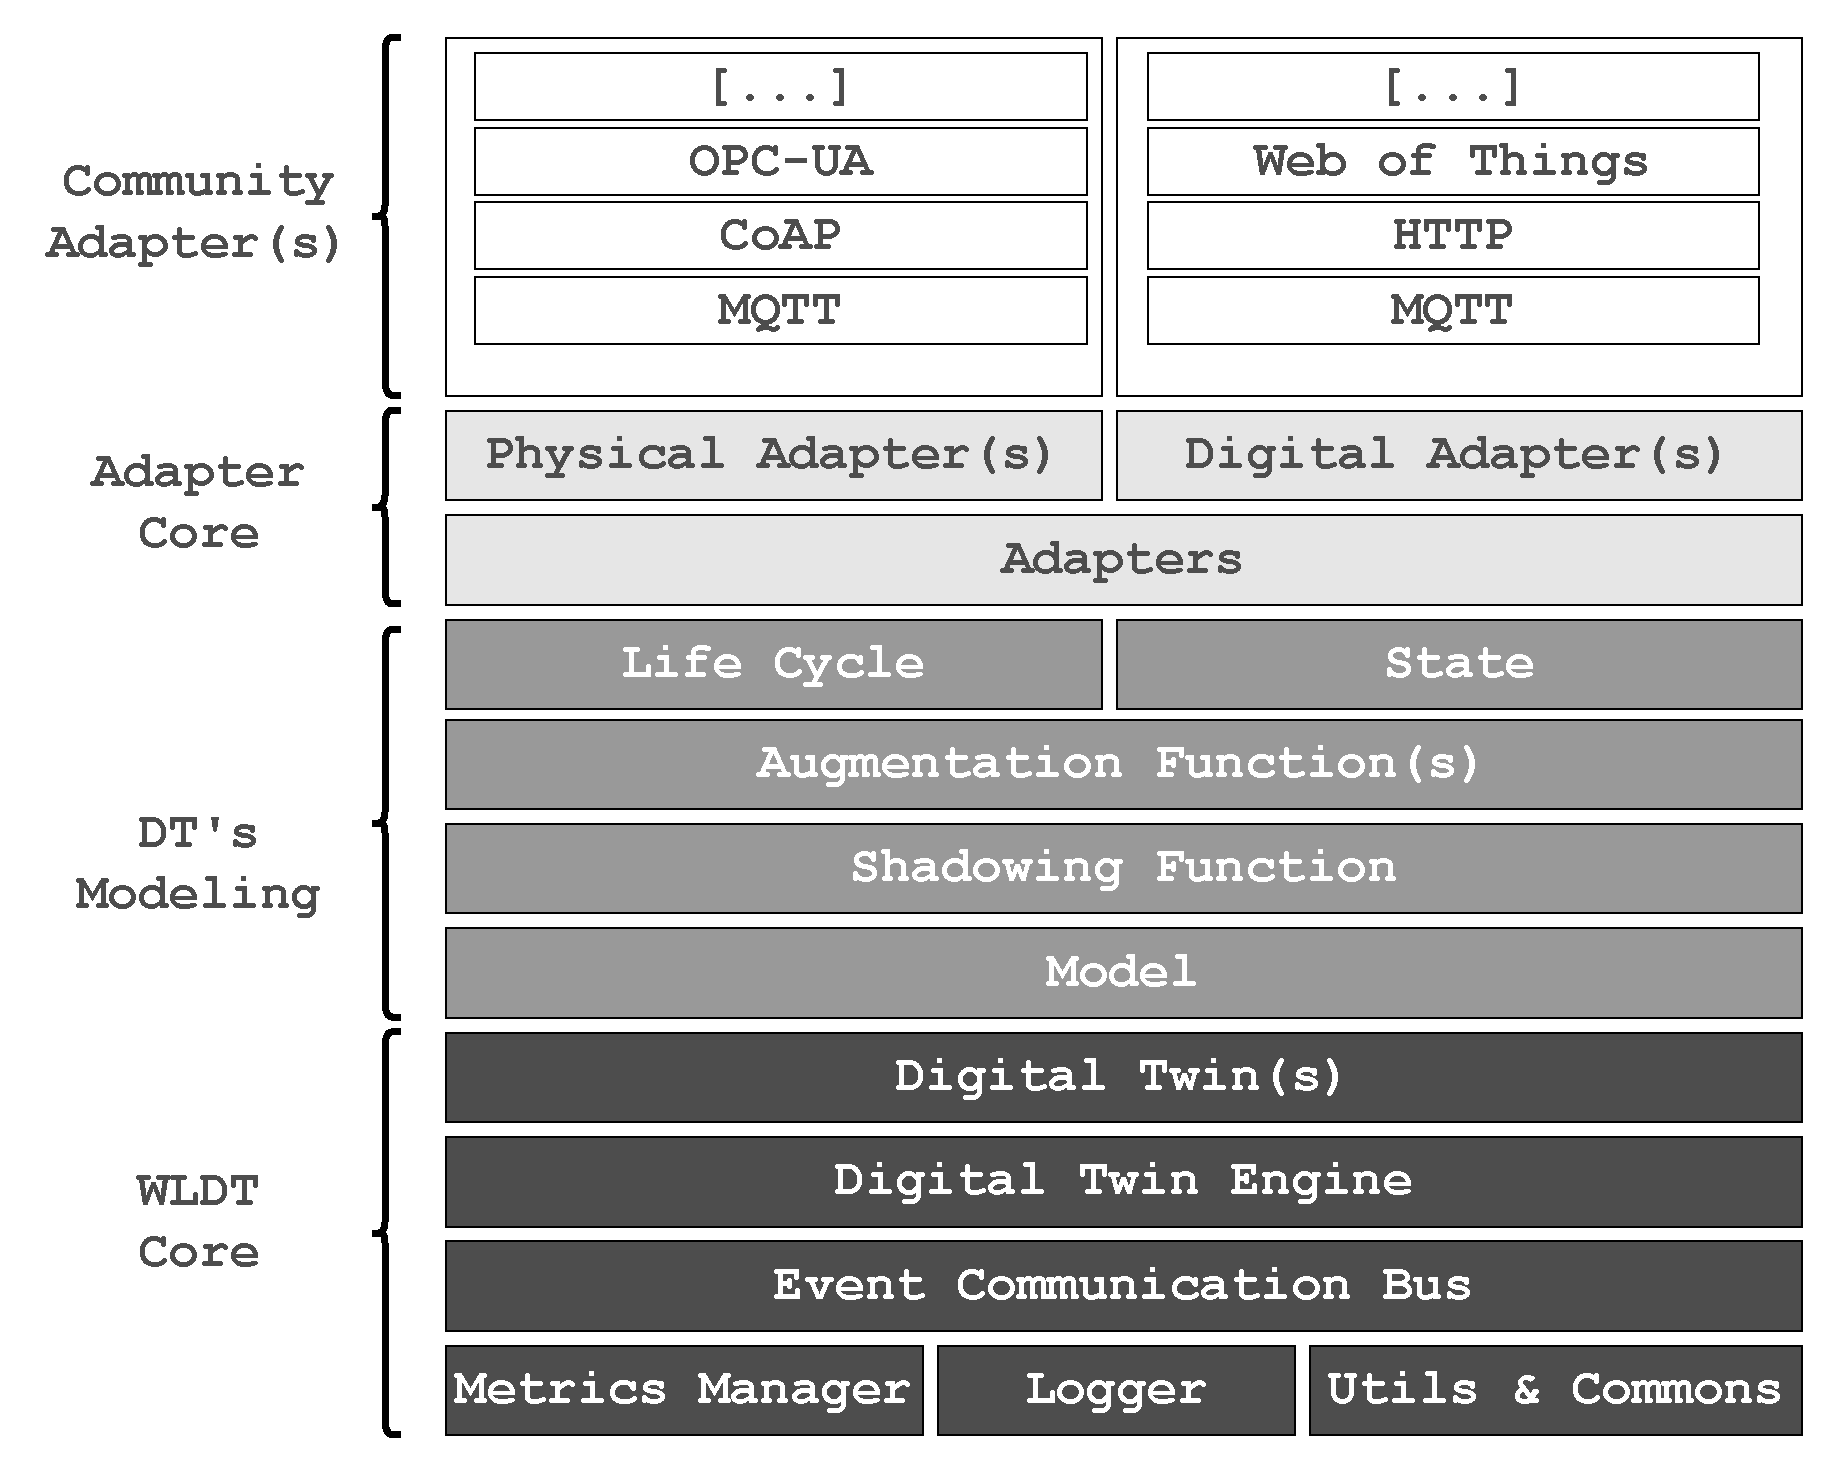
\includegraphics[width=0.7\textwidth]{figures/wldt_architecture.pdf}
    \caption{WLDT Framework's Software Architecture.}
    \label{fig:wldt_architecture}
\end{figure}

The concepts introduced in the previous sections have been implemented in an extended and evolved version of the \acf{WLDT} framework (originally introduced in \cite{PICONE2021100661}) offering a modular DT software architecture designed to maximize flexibility, promote portability, and enable seamless integration across diverse physical assets in diverse application domains.
%
\ac{WLDT} is an open-source Java framework available on GitHub\footnote{\url{https://wldt.github.io}}.

The \ac{WLDT} framework has been re-designed and extended with key requirements:
\begin{itemize}
    \item \textbf{Simplicity}: to facilitate the creation of \ac{DT} instances using existing modules or custom behaviors for specific scenarios;
    \item \textbf{Extensibility}: to allow easy extension of the \ac{DT} \ac{API}, enabling customization and addition of new features through concurrent module execution;
    \item \textbf{Portability \& Microservice Readiness}: to ensure that \ac{DT}s can run on any platform without modifications, supporting deployment as independent microservices.
\end{itemize}

The main components of the \ac{WLDT} architecture are illustrated in \Cref{fig:wldt_architecture}, which outlines the three architectural levels: the core library, the DT model, and the implementation of physical and digital interfaces through \ac{PhA} and \ac{DiA} (\Cref{sec:dte:engineering-dt:physical-digital-adapters}).

The \textit{Metrics Manager} provides the functionalities for managing and tracking various metrics within DT instances, combining both internal and custom metrics through a flexible and extensible approach.
The \textit{Logger} is designed to facilitate efficient and customizable logging within implemented and deployed DTs, with configurable log levels and versatile output options.
The \textit{Utils \& Commons} component contains a collection of utility classes and common functionalities that can be readily employed across DT implementations, ranging from handling common data structures to providing helpful tools for string manipulation.

The \textit{Event Communication Bus} represents the internal Event Bus, designed to support communication between the different components of the \ac{DT} instance (\ac{PI}, \ac{M} and \ac{DI}).
%
It allows for the definition of customized events to model both physical and digital inputs and outputs. Each \ac{WLDT} component can publish on the shared Event Bus and define a filter to specify which types of events it is interested in managing, associating a specific callback to process different messages.

The \textit{Digital Twin Engine} defines the multi-threaded engine of the library, allowing the execution and monitoring of multiple \acp{DT} and their core components simultaneously.
It orchestrates the different internal modules of the architecture while keeping track of each one, and it serves as the core of the platform, enabling the execution and control of deployed \acp{DT}.
Currently, it supports the execution of multiple twins within the same Java process, but the same engine abstraction could extend the framework to support distributed execution through different processes or microservices.

The DT component consists of a modular structure within \ac{WLDT}, combining core functionalities and capabilities of physical and digital adapters.
%
Each DT's core module is its \textit{Model}, which is responsible for implementing the twin's behavior over time. This model controls both the \textit{Shadowing Function} and \textit{Augmentation Function(s)}.
%
The Shadowing Function manages the digitalization process by integrating data from physical adapters and action requests from digital adapters.
It maintains the DT's \textit{State}, organizing properties, events, actions, and relationships as introduced in \Cref{sec:dte:engineering-dt:abstract-architecture}.
%
Augmentation Functions enhance physical capabilities by introducing new properties and actions through intelligent functionalities or dedicated processing (e.g., anomaly detection or data aggregation).
The DT's core is managed by the library to ensure consistency and lifecycle management, adapting to computational phases and interactions with physical and digital realms via adapters. 

\ac{WLDT} implements functionalities to manage the \ac{DT} synchronization lifecycle as described in \Cref{sec:dte:engineering-dt:dt-lifecycle}, ensuring proper transitions between phases and maintaining alignment with the physical asset's lifecycle.
%
Within the \ac{DT} core, the \emph{Shadowing Function} is responsible for receiving \acp{PAD} from \acp{PhA} and processing them to define when the \ac{DT} can be considered correctly \texttt{Bound} and when the \ac{DT} can be considered \texttt{Synchronized}, starting the \ac{DT} state computation. 

Developers can either leverage existing adapters---customized through configuration for context-specific reuse---or create new ones tailored to their specific requirements.
Each adapter has an internal dedicated lifecycle within the DT to ensure it can start, setup the necessary resources and respond to incoming events appropriately.
%
Adapters are identified by unique IDs, enabling the library to coordinate multiple adapters, adjust logs, and execute functions upon receiving new events. 
%
\ac{DiA} have direct access to the \ac{DT}'s state as well as the \ac{DT} history through callbacks or synchronous access, allowing it to retrieve information and expose it to digital consumers through various protocols according to the application context.


%========================================================
\section{Evaluation of the Proposed Approach}
%========================================================

In this section, the proposed architectural approach for engineering \acp{DT} is evaluated through the implementation of an industrial scenario.
%
This showcase demonstrates the practical application of the concepts introduced in the previous sections and highlights the benefits and challenges of the approach in a real-world context.

%-------------------------------------------
\subsection{Industrial Scenario Description}
 \label{ssec:dte:dt-engineering:scenario}
%-------------------------------------------

As a reference scenario, a manufacturing setting where \ac{DT} are deployed to monitor and manage a production line is considered. 
%
The production line is realized through the \emph{Fischertechnik Training Factory Industry 4.0}\footnote{Fischertechnik Industry \& Universities: \url{https://www.fischertechnik.de/en/products/industry-and-universities}}, controlled by PLCs that publish real-time data via OPC-UA and integrated with Arduino RP2040 boards\footnote{Arduino RP2040: \url{https://docs.arduino.cc/hardware/nano-rp2040-connect/}} for accelerometer data collection and processing and communicating over MQTT.
The schematic representation of the microfactory production line is shown in \Cref{fig:microfactory-production-line}.
This microfactory setup provides a controlled yet dynamic environment for testing and refining DT technologies in a realistic industrial context.

\begin{figure}[t]
    \centering
    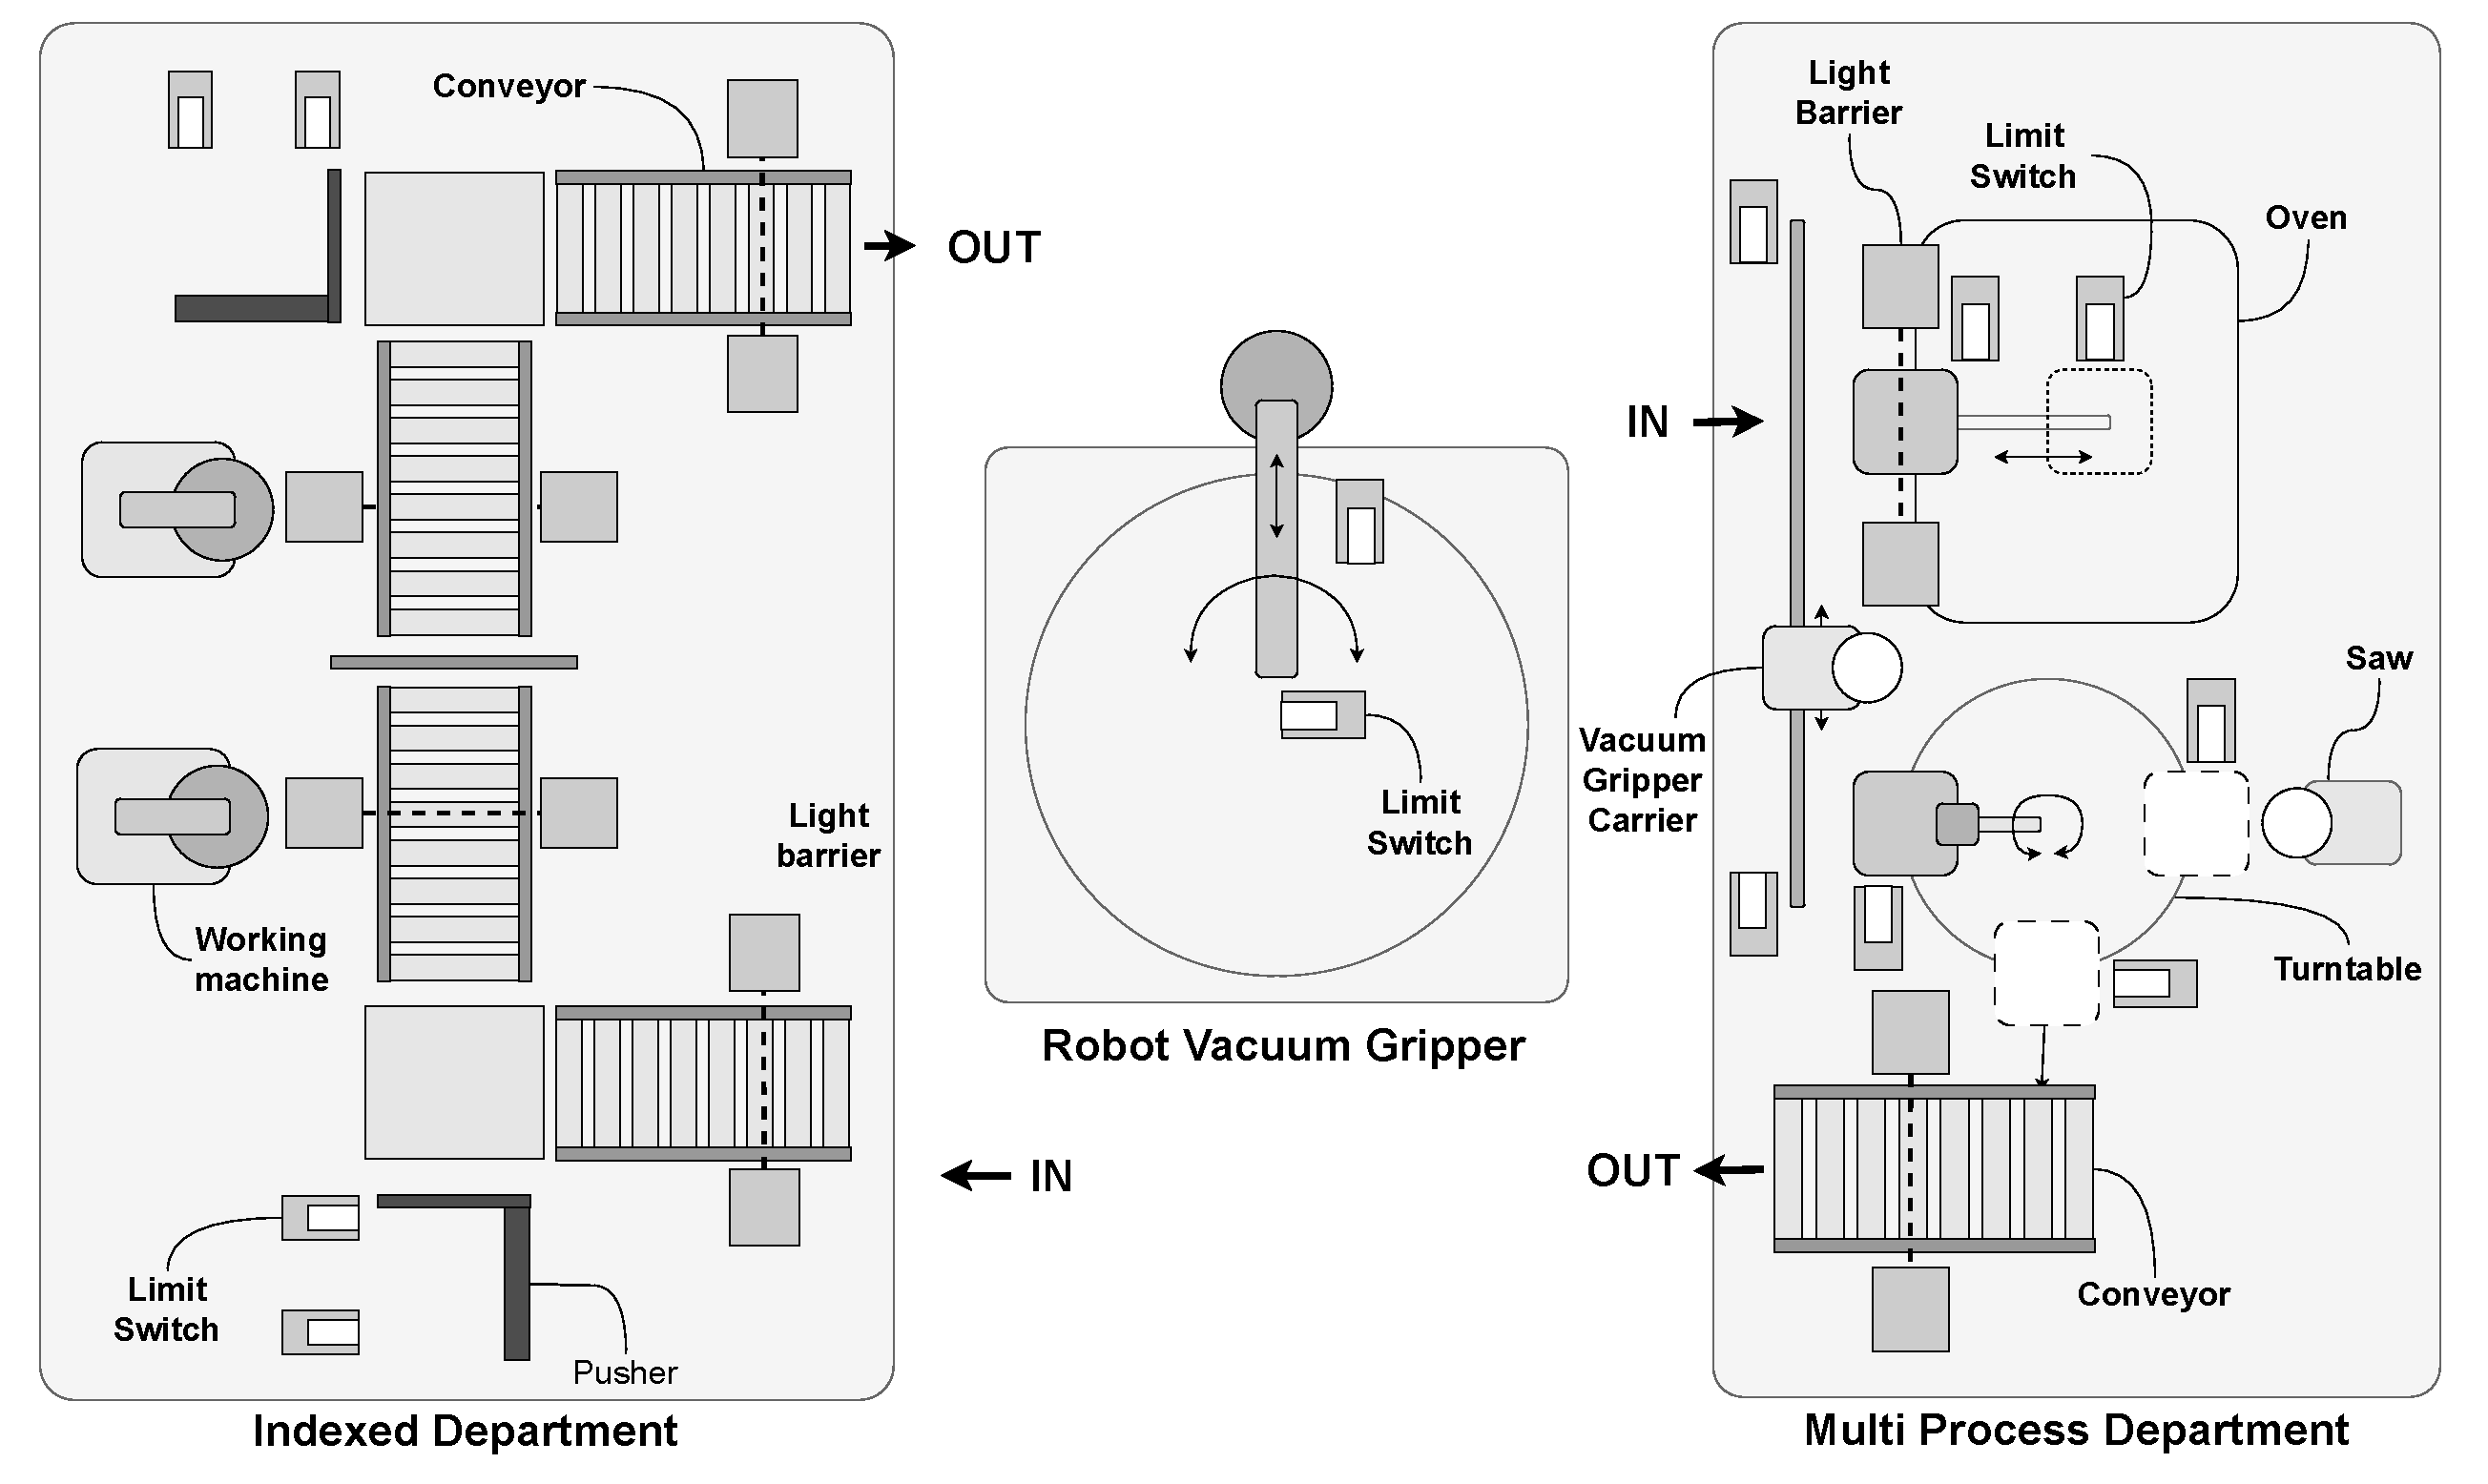
\includegraphics[width=0.8\columnwidth]{figures/mf_highlevel_schema.pdf}
    \caption{A schematic view of the microfactory production line, with the two departments.}
    \label{fig:microfactory-production-line}
\end{figure}

In this scenario, pieces are processed along a production line, passing through multiple machines.
%
The first station, referred to as the \textit{Multiprocess Station with Oven}.
As shown in \Cref{fig:microfactory-production-line} (right), the module consists of five machines arranged in a flow shop layout: 
three material handling units (vacuum gripper carrier, turntable, and conveyor)
and two transformation stations (oven and saw station).
%
Each machine is equipped with sensors (light barriers and limit switches) and actuators (with two or three operational states).
%
The second station, named the \textit{Indexed Line} (\Cref{fig:microfactory-production-line}, left), comprises four conveyor belts, two of which include mechanical processing operations for the workpieces.

The goal of the scenario is to implement, through \acp{DT}, a system with the following desired features: 
\begin{itemize}
    \item monitor the state of each machine in the production line;
    \item track production performance, including the number of pieces processed and the efficiency of each machine;
    \item monitor power consumption of each machine to optimize energy usage;
    \item regulate the production speed of each machine to ensure smooth operation and avoid bottlenecks;
    \item compute the overall production performance of the entire production line;
    \item compute the overall energy consumption of the entire production line;
    \item manage external action requests, at the system level, to adjust production parameters or respond to specific events;
\end{itemize} 

%--------------------------------------------
\subsection{Digital Twin System Architecture}
%--------------------------------------------

To achieve the desired features, a multi-layered architecture is proposed, consisting of machine-level, department-level, and factory-level \acp{DT}.
%
Each machine-level \ac{DT} processes incoming data on properties and events to generate insights such as production and energy KPIs, while also managing action requests to regulate their individual speed.
%
Additionally, two department-level \acp{DT} are created, matching the two different goals of tracking energy consumption and production performance.
%
All \acp{DT} are built using the \ac{WLDT} framework.

The production efficiency is computed at the machine level using the \ac{OEE} metric\footnote{OEE: \url{https://www.oee.com/}} calculated from production rate, uptime, and downtime.
%
At the department level, \acp{DT} representing the Indexed Departments assess performance by computing Weighted \ac{OEE}~\cite{OEE-manufacturing-cell-Gamberini-2017,Introduction-to-TPM-total-productive-maintenance-Nakajima-1995}, derived from individual machine \acp{DT}, and track throughput, defined as processed pieces per unit time.
Throughput is determined by monitoring entry and exit events within the department, utilizing relationships captured by the associated \acp{DT}.

\begin{figure}
    \centering
    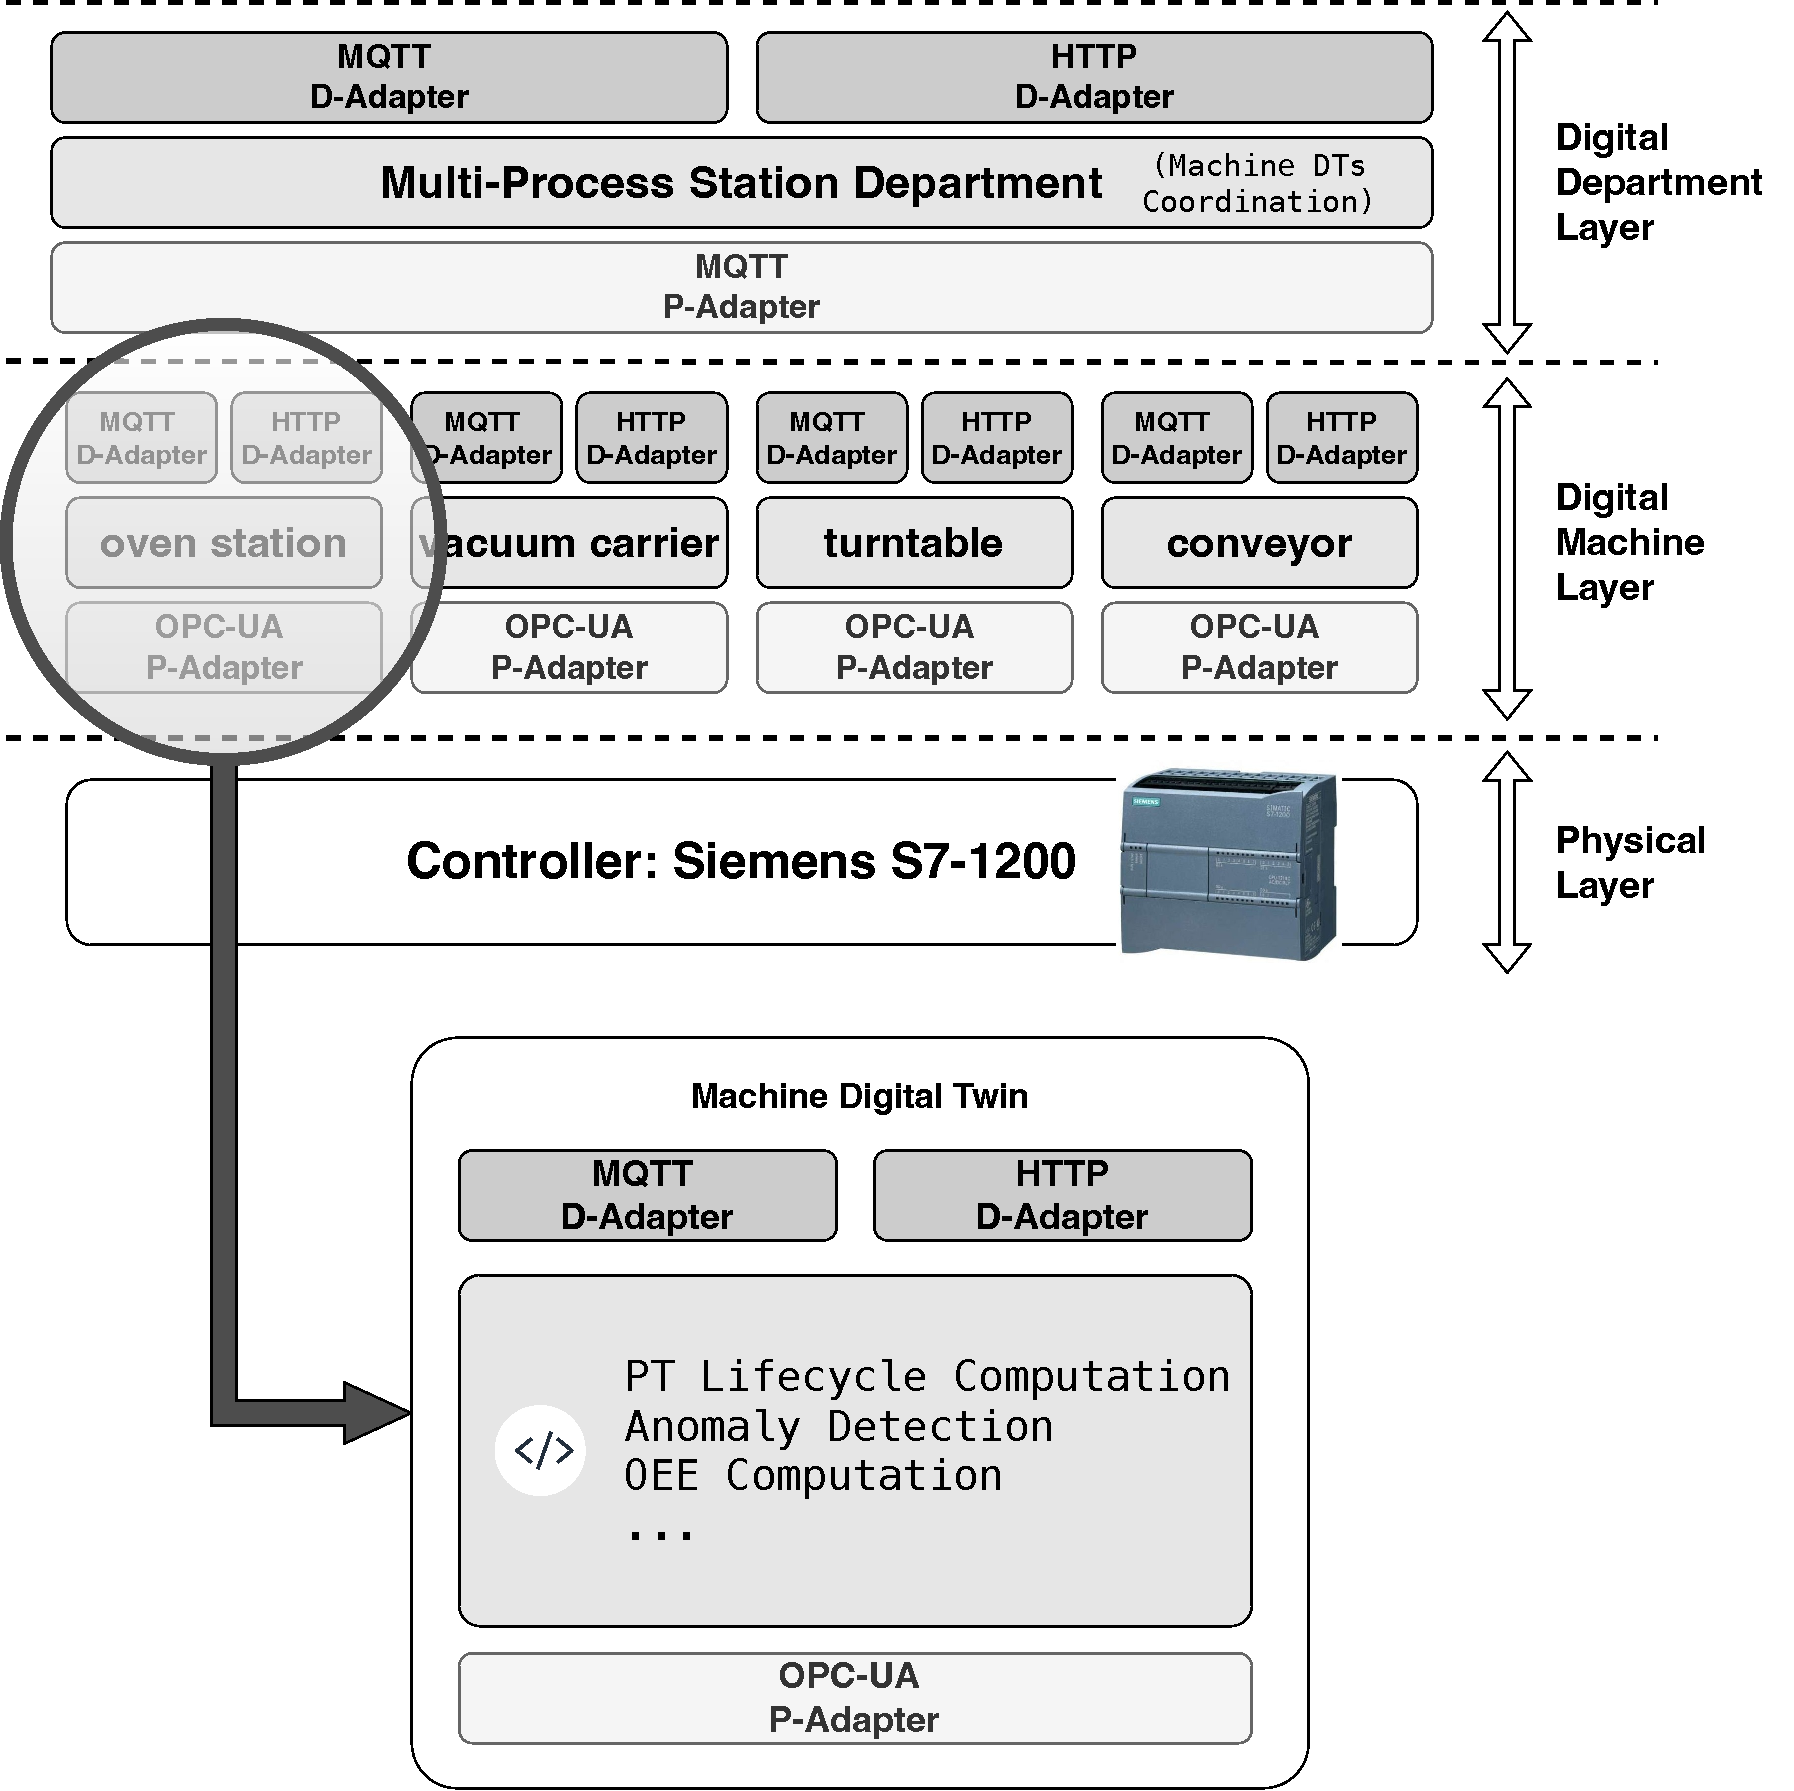
\includegraphics[width=0.7\textwidth]{figures/dt-lifecycle/mps_dt_structure_2.pdf}
    \caption{Multiprocess Station Digital Twin architecture overview.}
    \label{fig:multiprocess-station-dt-structure}
\end{figure}

\Cref{fig:multiprocess-station-dt-structure} shows the resulting \ac{DT} system architecture for the \textit{Multiprocess Station with Oven}.
%
Each machine of the station is represented by a dedicated \ac{DT} which connects to the physical asset through a \ac{PhA} that interacts with the PLC iva OPC-UA.
%
At the department level, the \ac{DT} of the \textit{Multiprocess Station with Oven} aggregates data from the machine-level \acp{DT}, computing overall performance metrics and exposing department-level actions.

\begin{figure}
    \centering
    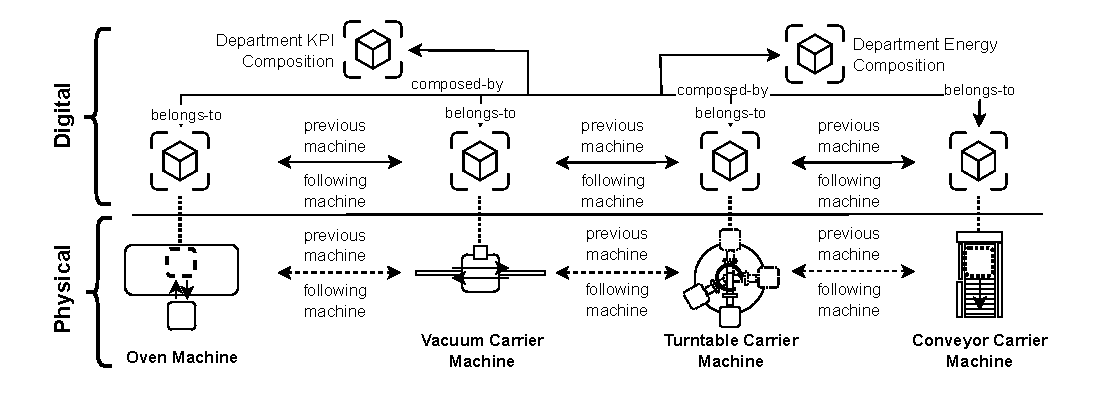
\includegraphics[width=\textwidth]{figures/engineering-wldt/Fischer-relationships.pdf}
    \caption{Relationships between \acp{DT} in the Multiprocess Station serve the purpose of tracking the physical relationships between different machines at the digital level.}
    \label{fig:dt-assets-relationships-overview}
\end{figure}

Figure \Cref{fig:dt-assets-relationships-overview} illustrates the relationships among the various \acp{DT} in the Multiprocess Station.
%
Relationships between machines and DTs (e.g., \emph{previous}, \emph{following-machines}, \emph{is-part-of}) are statically defined in this setting, but are used by department-level \acp{DT} do track the flow of pieces and compute throughput and total pieces processed.
%
\begin{figure}
    \centering
    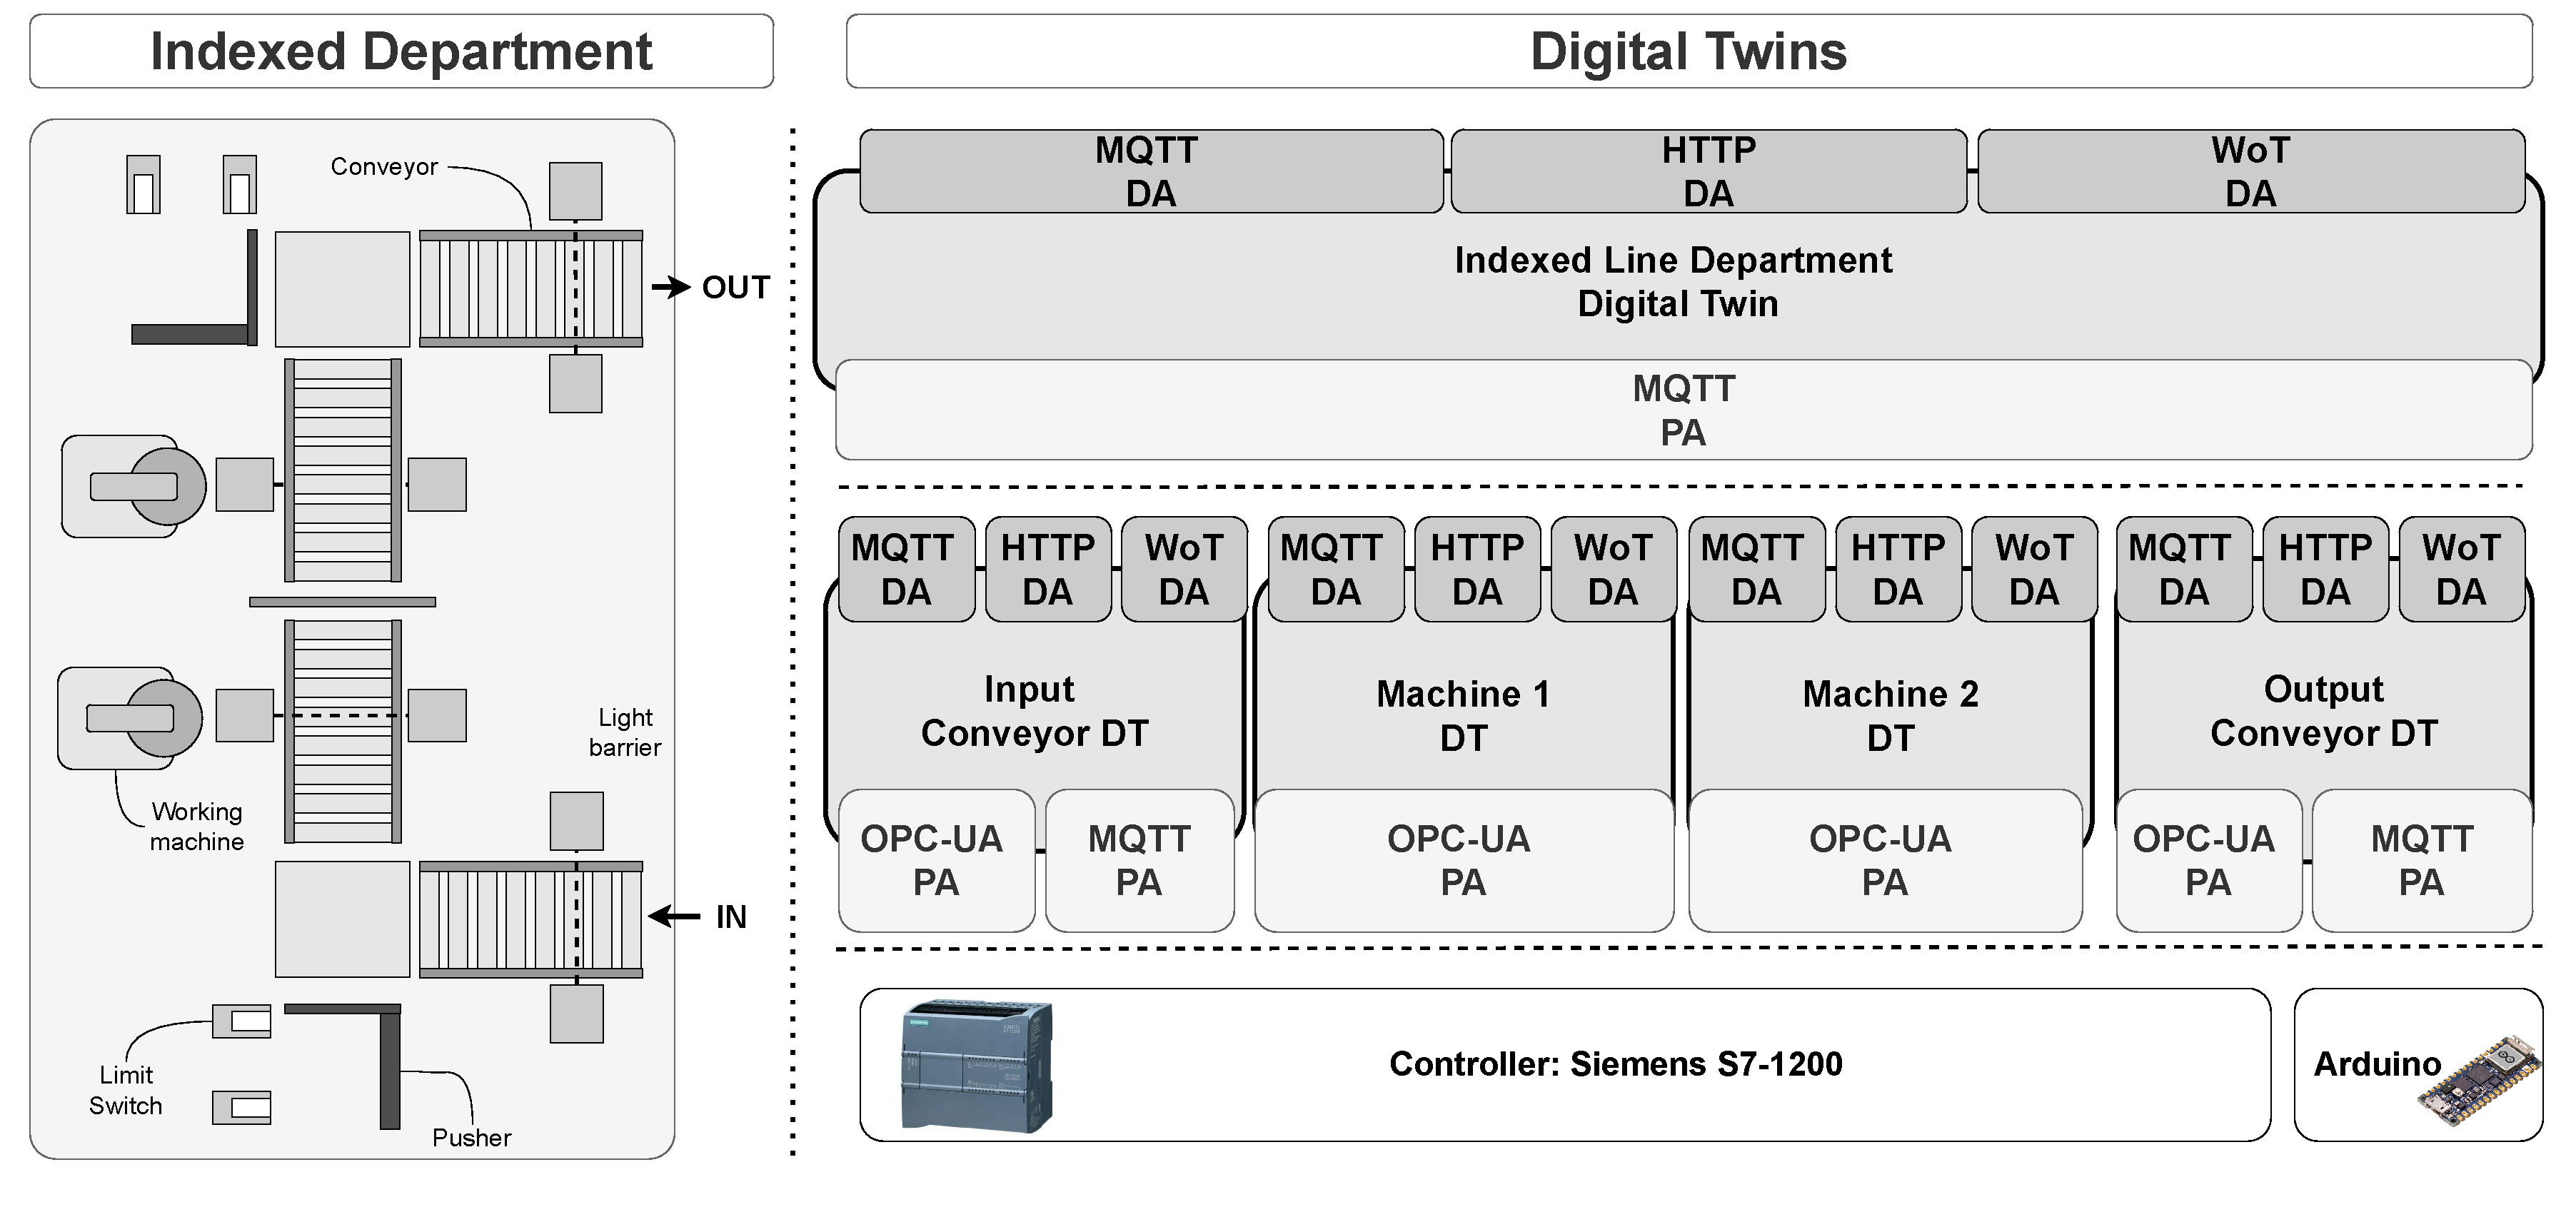
\includegraphics[width=\textwidth]{figures/dt-interoperability/mf_dt_structure.pdf}
    \caption{The \acl{DT} ecosystem architecture of the Indexed Department, alongside a schematic representation of the conveyors.}
    \label{fig:indexed-department-dt-structure}
\end{figure}

Similarly, \Cref{fig:indexed-department-dt-structure} illustrates the \ac{DT} ecosystem architecture for the \textit{Indexed Line Department}. Again, each machine is represented by a dedicated \ac{DT} connected to the physical asset through \acp{PhA}. In this setup, machines integrate the communication of the PLC via OPC-UA and Arduino boards via MQTT.
%
Finally, a factory-level \ac{DT} aggregates data from both departments, 
computing the overall production performance and energy consumption.


Machine Level \acp{DT} expose a digital interface through \acp{DiA}. 
%
An MQTT digital interface is used to connect machine-level \acp{DT} to the department-level \ac{DT}, enabling composition between \acp{DT} in a hierarchical structure. 
%
All \acp{DT} also expose an \ac{HTTP} digital interface which serves as the primary access point for external applications and services.
%
The \ac{HTTP} interface can further be described using \ac{WoT} \acp{TD}, enabling seamless integration with other \ac{WoT}-compliant systems and applications as discussed in \Cref{sec:dte:dt-engineering:wot-for-dt}.

%-------------------------------------------------------------------------
\subsection{Reducing Complexity through Reusable Adapters}
%-------------------------------------------------------------------------

Notably, the physical and digital adapters that implement MQTT, OPC-UA, and HTTP protocols, along with \ac{WoT} over HTTP for serving \acp{TD}, are reusable across different instances.
These adapters, through configurable parameters, enable effective communication and integration within both digital and physical environments.

Upon startup, each \ac{DT} connects to its data source, publishes the \ac{PAD} of the physical asset, and interacts with the PLC or Arduino to collect and send data, enabling digitalization and interoperability among heterogeneous equipment. 

%%%
\begin{figure}
    \centering
    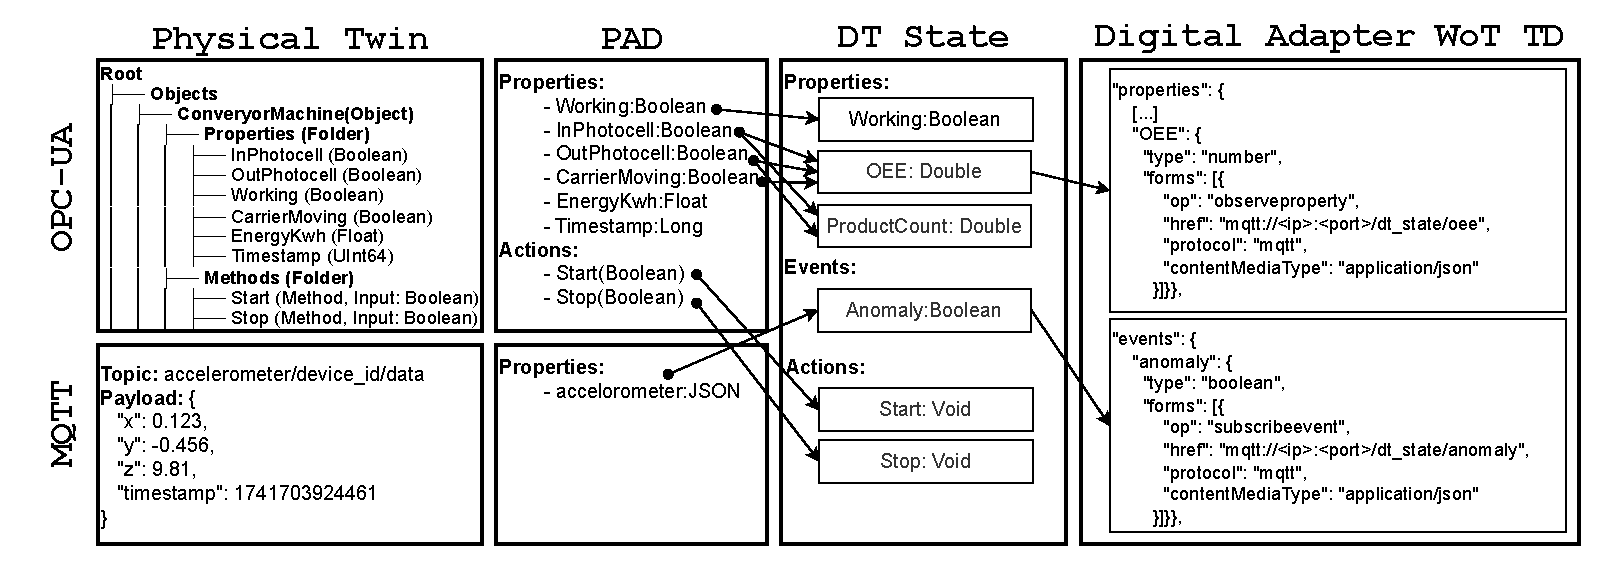
\includegraphics[width=\textwidth]{figures/dt-interoperability/dt_interoperability-pad_dt_wot.pdf}
    \caption{The transition from physical to digital representation via the \ac{PAD}, the \ac{DT} State, and the \ac{DTD} for external consumers.}
    \label{fig:pad_dt_wot}
\end{figure}
%%%


\Cref{fig:pad_dt_wot} schematically illustrates the evolution of data and representation from the physical to the digital realms through the adoption of the proposed \ac{DT} architectural approach, \ac{PAD} integration, and \ac{WoT} \acp{TD} used as \acp{DTD} on the digital side, specifically for the output conveyor of the Indexed Department production line (\Cref{fig:indexed-department-dt-structure}).
On the physical side, data is structured using OPC-UA with a hierarchical organization, containing telemetry data and action methods mapped to specific data types.
Accelerometer data is transmitted over MQTT on a specific topic with a JSON payload containing axis acceleration values. 

The \acp{PAD} act as an intermediary, translating data from the PT into a format suitable for the DT core, decoupling it from the complexity of interacting with the \ac{PT} and enabling discovery, understanding, and utilization of available data and methods.
Using the information from the \acp{PAD}, the \ac{DT} model computes the \ac{DT}'s state with target properties, events, and actions, based on either one-to-one matching of physical characteristics or augmented by combining multiple physical properties into computed \ac{DT} properties or events, such as computing the value of the \ac{OEE} property or triggering anomaly detection events based on accelerometer data. 

Finally, the \ac{DiA} of the \ac{DT} leverages \ac{WoT} \ac{TD} to describe the DT's data and functionalities through a standardized, interoperable, and machine-readable approach.
The \ac{TD} specifies how these can be accessed via protocols and data formats.
This approach enables effective interoperability from the physical to the digital, using a modular and decoupled structure through \acp{DT} in the target industrial use case.

This deployment aims to measure the impact of digitization and responsibility decoupling by comparing the system complexity in scenarios with and without \ac{DT} adoption and also with respect to the different \ac{DT}'s architectural layers.
%
This allows to assess the benefits of a modular, structured DT-based approach, particularly in terms of interoperability and heterogeneity management.

To quantify how effectively the proposed approach of \ac{PhA} and \ac{DiA} manages cyber-physical heterogeneity,
the \textit{Cyber-Physical Complexity Index (CP-CI)} proposed in \cite{lippi_dt_causality_learning, LOMBARDO2024107203} is adopted as a measure of complexity of the system. 

The CP-CI quantifies the perceived complexity of a cyber-physical application based on:
\begin{itemize}
    \item \textit{Required Protocols (p)}: communication protocols needed for device interaction;
    \item \textit{Communication Patterns (c)}: interaction models (e.g., Publish/Subscribe, Request/Response);
    \item \textit{Data Formats (d)}: required data representations or serialization methods;
    \item \textit{Interaction Points (n)}: modules or services involved in data exchange; and
    \item \textit{Aggregation Points (a)}: levels of abstraction for physical data (e.g., merging data from multiple machines).
\end{itemize}
Each criterion is weighted with a \textit{Criteria Importance Factor} (\(CIF\)) from 1 (low) to 3 (high), indicating its impact on development, deployment, and maintenance.

Focusing on \ac{DT} interoperability, the CP-CI is extended to include both inbound and outbound interfaces, essential for bridging the physical and cyber layers with differing requirements.
This extension enables a more precise assessment of the complexity in managing interoperability across system boundaries.
The CP-CI was applied not only to the entire \ac{DT} but also to its internal layers: \ac{PI}, Core, and \ac{DI}.
These results were compared to those of a monolithic external application that directly handles business logic and interoperability, bearing the full complexity, highlighting the advantages of the modular \ac{DT} design.
High importance ($CIF=3$) was assigned to managing heterogeneous data formats ($d$) and aggregation points ($a$), as they are crucial for creating interoperable data models.
Medium importance ($CIF=2$) was given to protocol diversity ($p$) and interaction with multiple entities ($n$), which become more significant as systems scale.
Low importance ($CIF=1$) was assigned to multiple communication patterns ($c$), as their concurrent use is standard in distributed applications.


\begin{figure}
  \centering
  \begin{subfigure}[t]{0.32\linewidth}
      \centering
      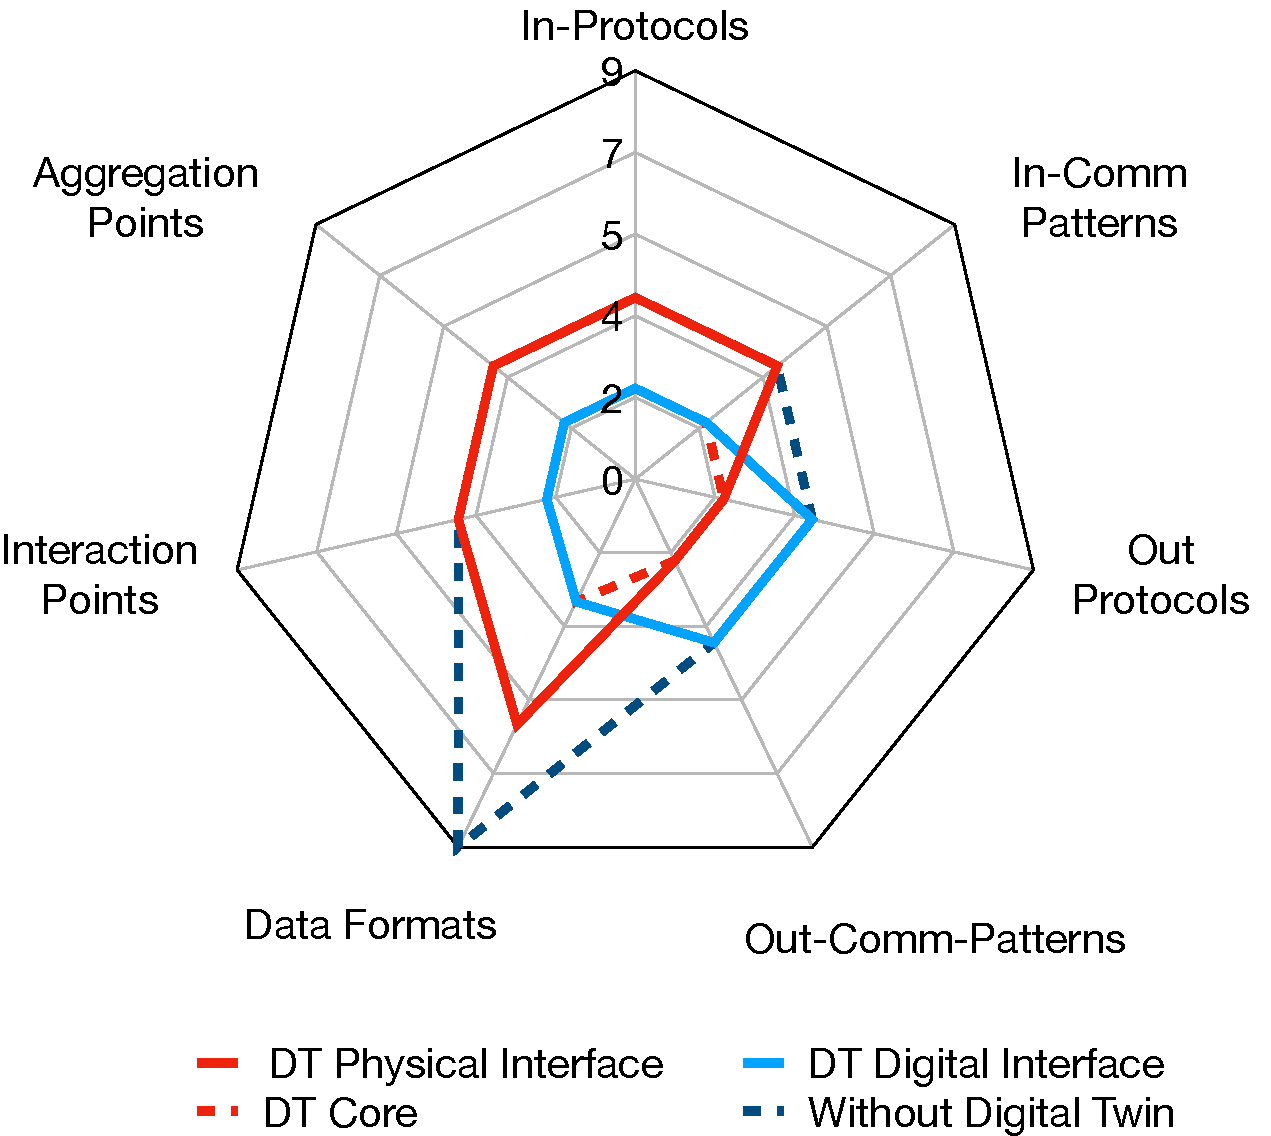
\includegraphics[width=\linewidth]{figures/dt-interoperability/machine_complexity_index.pdf}
      \caption{Machine Digital Twin}
      \label{fig:machine_complexity_index}
  \end{subfigure}
  \begin{subfigure}[t]{0.32\linewidth}
      \centering
      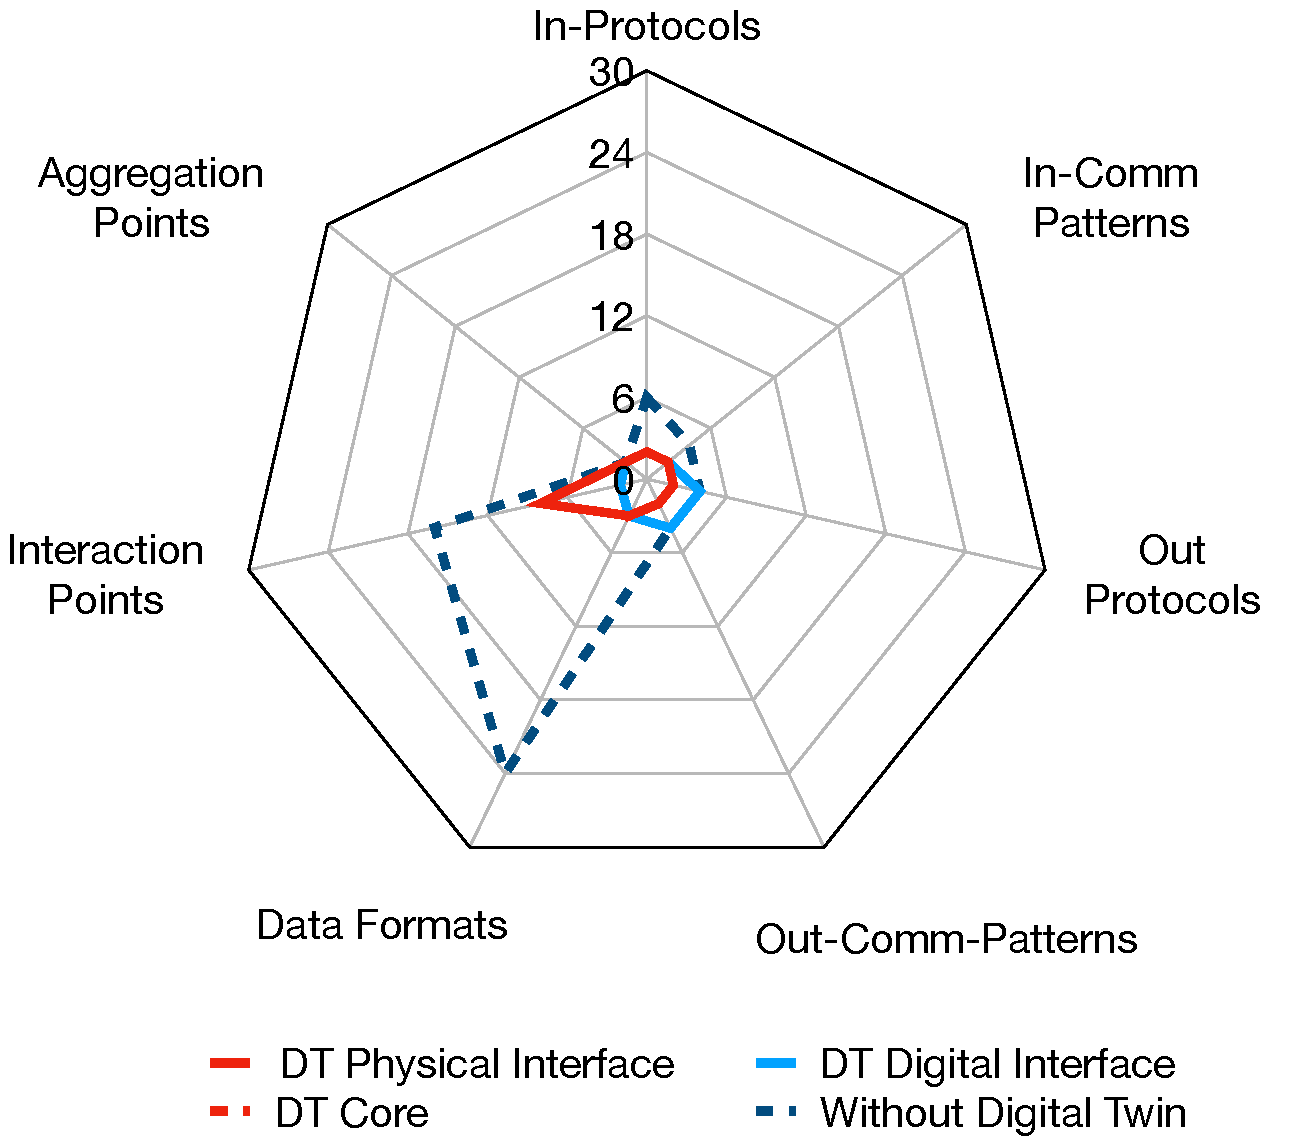
\includegraphics[width=\linewidth]{figures/dt-interoperability/station_complexity_index.pdf}
      \caption{Station (Indexed-Line) Digital Twin}
      \label{fig:station_complexity_index}
  \end{subfigure}
  \begin{subfigure}[t]{0.32\linewidth}
      \centering
      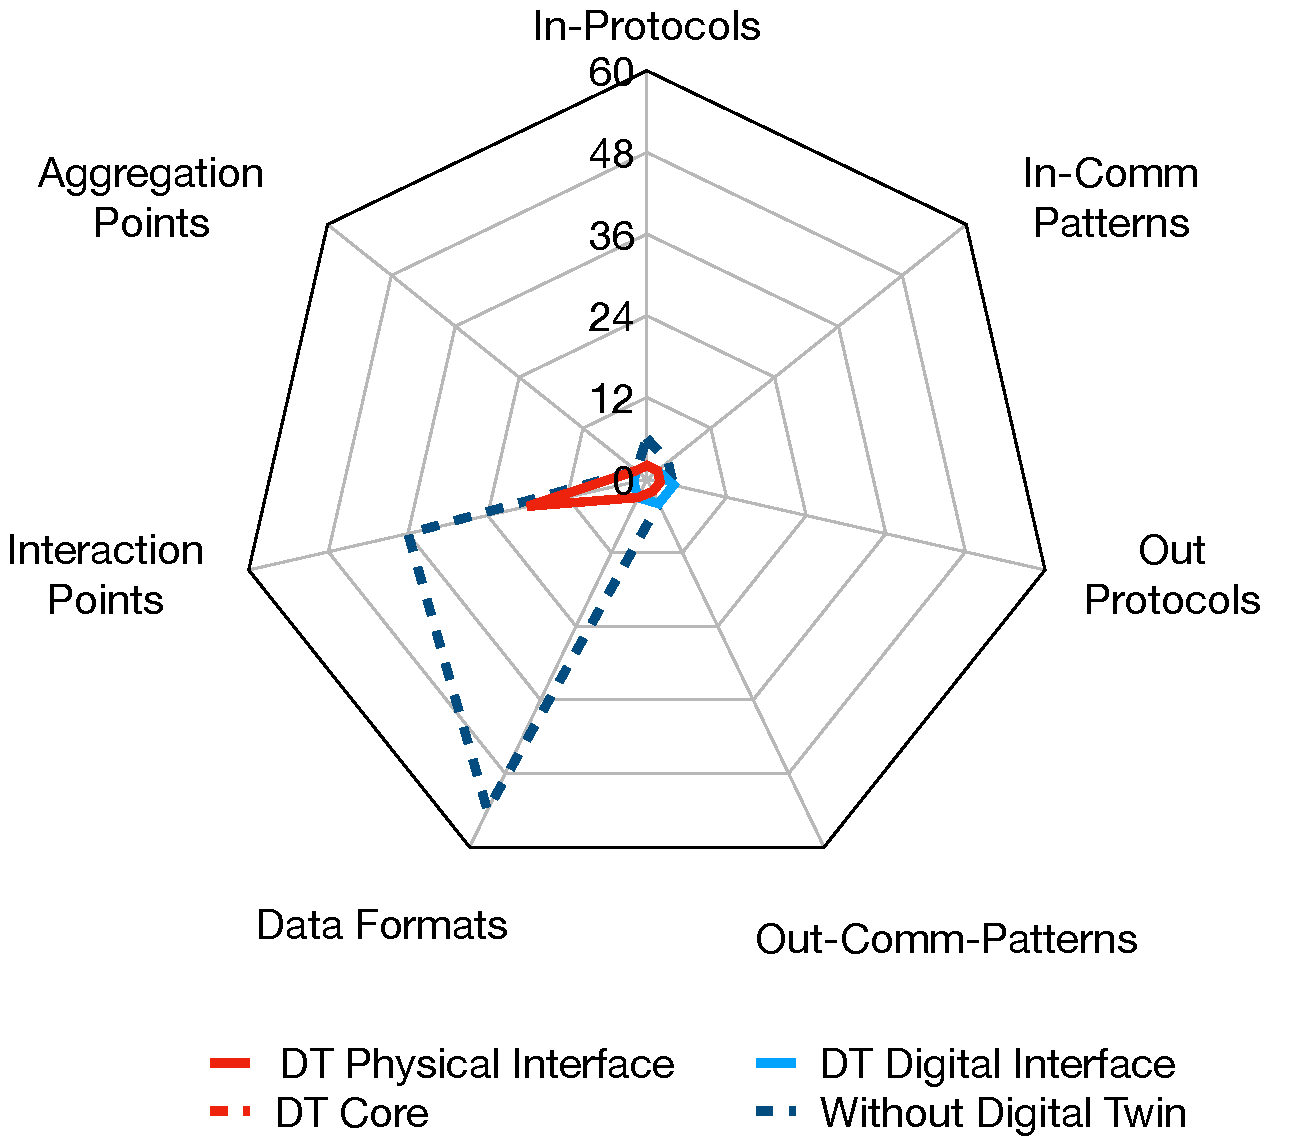
\includegraphics[width=\linewidth]{figures/dt-interoperability/factory_complexity_index.pdf}
      \caption{Factory Digital Twin}
      \label{fig:factory_complexity_index}
  \end{subfigure}
  \caption{Schematic representation of cyber-physical complexity and its impact on various components.}
  \label{fig:dt_complexity_index}
\end{figure}


The graphs presented in \Cref{fig:dt_complexity_index} display the CP-CI values obtained across different levels of deployment: a single machine, the indexed department, and the entire factory.
%
For the machines analyzed, the involved protocols ($p$) and communication patterns ($c$) are both set to 2, as MQTT and OPC-UA are used with Pub/Sub and Request/Response interactions.
On the digital side, both MQTT and HTTP are employed.
Regarding data formats ($d$), each machine manages 2 distinct formats, accounting for both PLC data and Arduino accelerometer information.
Furthermore, the interaction points ($n$) and aggregation points ($a$) are both 2, reflecting the aggregation and interaction with two different sub-entities for each machine and its corresponding DT.

The results for single machines (\Cref{fig:machine_complexity_index}) highlight the critical role of the \ac{PI} in the \ac{DT} architecture.
As a decoupling layer, the \ac{PI} isolates physical-world complexities from the DT core, managing priorities like protocols, data formats, interaction points, aggregation strategies, and communication patterns.
This allows the DT core to focus on uniform data, processed through the interface via \ac{PAD} and payload transformations, without dealing with heterogeneous physical entities.
%
Consequently, the core interacts only with its internal communication pattern and consistent interaction points, regardless of the physical environment's configuration.
A similar approach is applied to the \ac{DI}, which is decoupled from physical complexities and adapts to external digital systems, ensuring modularity and reuse.

In contrast, systems without a \ac{DT} must embed all heterogeneity management into a single application, burdening it with business logic, protocol diversity, and data format interoperability.
This increases complexity and reduces scalability, as reflected by the complexity index parameters.

As system architecture scales from individual machines to departments (Figure \ref{fig:station_complexity_index}), or entire factories (Figure \ref{fig:factory_complexity_index}), protocol diversity stabilizes while the number of interaction points and data formats increases due to the need for managing heterogeneous components.
The complexity measure shows that systems at the department or factory level experience a significant rise in complexity, driven by interaction points, aggregation nodes, and data format diversity.

These results emphasize the benefits of the modular and interoperable approach presented in \cref{sec:dte:engineering-dt:physical-digital-adapters}.
By encapsulating complexity within reusable \emph{adapters} and using interoperable representations, developers can simplify application development.
In contrast, monolithic systems struggle with managing interoperability and system evolution as integration requirements grow.

%---------------------------------------------------
\subsection{Lifecycle Awareness and Coordination}
%---------------------------------------------------

To demonstrate the applicability of the proposed lifecycle synchronization model introduced in \cref{sec:dte:engineering-dt:dt-lifecycle}, 
each machine-level \ac{DT} handles the synchronization between the $LP_{PA}$ and the corresponding $LP_{DT}$.
%
Furthermore, an anomaly detection algorithm runs within each \ac{DT}, enabling it to identify and report issues that the PLC alone might not detect, thus dynamically computing the $LP_{PA}$ when necessary (e.g., when a piece does not reach a reference photocell on the machinery within a predetermined time and an anomaly is consequently detected).

The department-level \ac{DT} of the Multiprocess Station incorporates coordination logic that adjusts machine behavior based on their current phases, ensuring seamless station management.

\begin{figure}
    \centering
    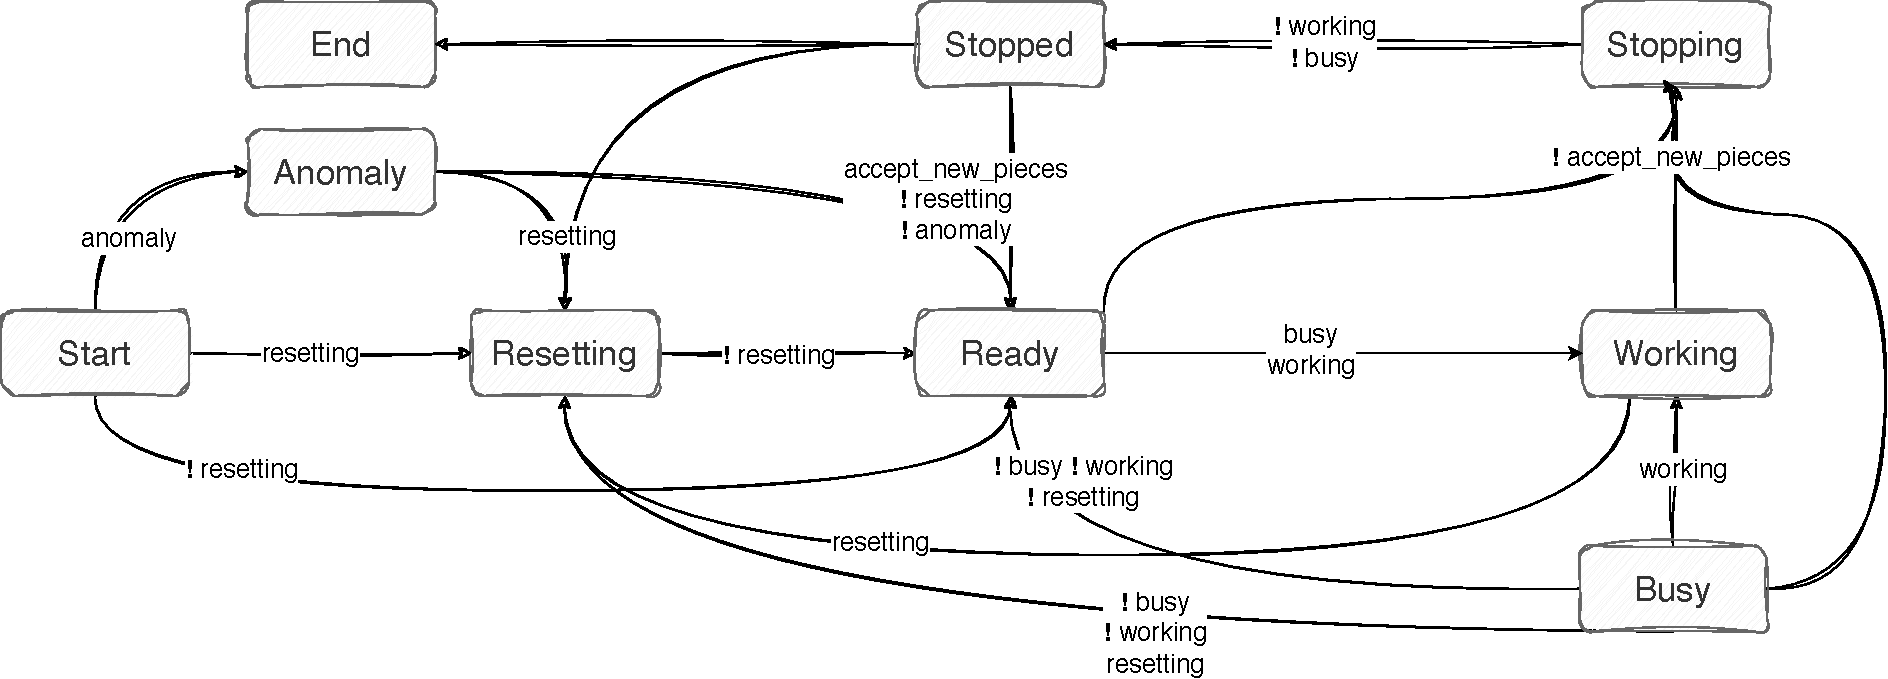
\includegraphics[width=\textwidth]{figures/dt-lifecycle/graph_machine_logic.pdf}
    \caption{Lifecycle of a \ac{PA} in the target industrial scenario, highlighting the different phases that the \ac{DT} needs to account for when synchronized.}
    \label{fig:graph-machine-logic}
\end{figure}

The machine-level \acp{DT} operate based on data produced by their physical counterparts. Leveraging these temporal data, it is possible to model the lifecycle of the physical object within the DT lifecycle as shown in \Cref{fig:graph-machine-logic}.
%
When the DT lifecycle reaches the Synchronized state, it accurately mirrors the corresponding phase of the physical machinery's operation.
%
These phases are inspired by the reference structure for industrial machine phases defined by ISA-95~\cite{ISA95} aligning \acp{DT} with recognized industry standards, enhancing their applicability and effectiveness in real-world industrial settings.

To accurately define the phases of the physical machinery,
it is essential to specify the transition conditions between these phases by leveraging the raw data and telemetry received from sensors and actuators via OPC-UA from the PLC.
%
The DT processes this data to compute and maintain the synchronized lifecycle, ensuring a precise and real-time reflection of the physical object's operational state.

Department-level \acp{DT} enable hierarchical coordination not only between machines within the same station but also across different stations.
%
For example, coordination between the \textit{Multiprocess Station} and the previously mentioned \textit{Indexed Line} can be simplified by establishing consistent lifecycle phases across machines.
%
Without this approach, coordination among multiple DTs requires using low-level physical information and telemetry, making the process less intuitive.

\begin{algorithm}
\caption{Multiple DTs Stopping Procedure}
\begin{algorithmic}
\State \texttt{invoke(OvenDT, STOP)}
\While{ \texttt{OvenDT.phase} \textbf{is not} \texttt{STOPPED} }
    \State \texttt{wait(OvenDT.phase} \textbf{is not} \texttt{WORKING)}
\EndWhile
%\vspace{1em}
%\State \textbf{publish} event ``change-vacuum-gripper-cycle" with value \texttt{false}
\State \texttt{invoke(GripperDT, STOP)}
\While{ \texttt{GripperDT.phase} \textbf{is not} \texttt{STOPPED}}
    %\State \textbf{log} waiting for end of vacuum-gripper \texttt{WORKING} state
    \State \texttt{wait(GripperDT.phase} \textbf{is not} \texttt{WORKING)}
\EndWhile
%\vspace{1em}
%\State \textbf{publish} event ``change-turntable-cycle" with value \texttt{false}
\State \texttt{invoke(TurntableDT, STOP)}
\While{ \texttt{TurntableDT.phase} \textbf{is not} \texttt{STOPPED} }
    %\State \textbf{log} waiting for end of turntable \texttt{WORKING} state
    \State \texttt{wait(TurntableDT.phase} \textbf{is not} \texttt{WORKING)}
\EndWhile
%\vspace{1em}
\State \texttt{invoke(OutputConveyorDT, STOP)}
\end{algorithmic}
\label{code:soft-stop-logic}
\end{algorithm}

As illustrated by \Cref{code:soft-stop-logic}, high-level control logic can be implemented directly leveraging information encapsulated by $LP_{DT}$ mapping the phase and the transitions of the associated physical counterparts $LP_{PA}$. Specifically, the algorithm outlines the steps the department-level DT can take to halt production on the multiprocess station.
By leveraging this additional layer of abstraction, the department-level DT no longer relies on raw sensor data for control operations, enabling a more declarative and effective coordination process, and distributing responsibilities across different DTs.
%
The composite DT leverages the PA lifecycle phases of individual machines to define the overall lifecycle of the entire multiprocess station. This provides a comprehensive overview of each station's operational behavior, enabling more effective and intuitive system management.


%-------------------------------------
\subsection{Performance Evaluation}
%-------------------------------------


\begin{figure}
    \centering
    \begin{subfigure}{0.75\textwidth}
        \centering
        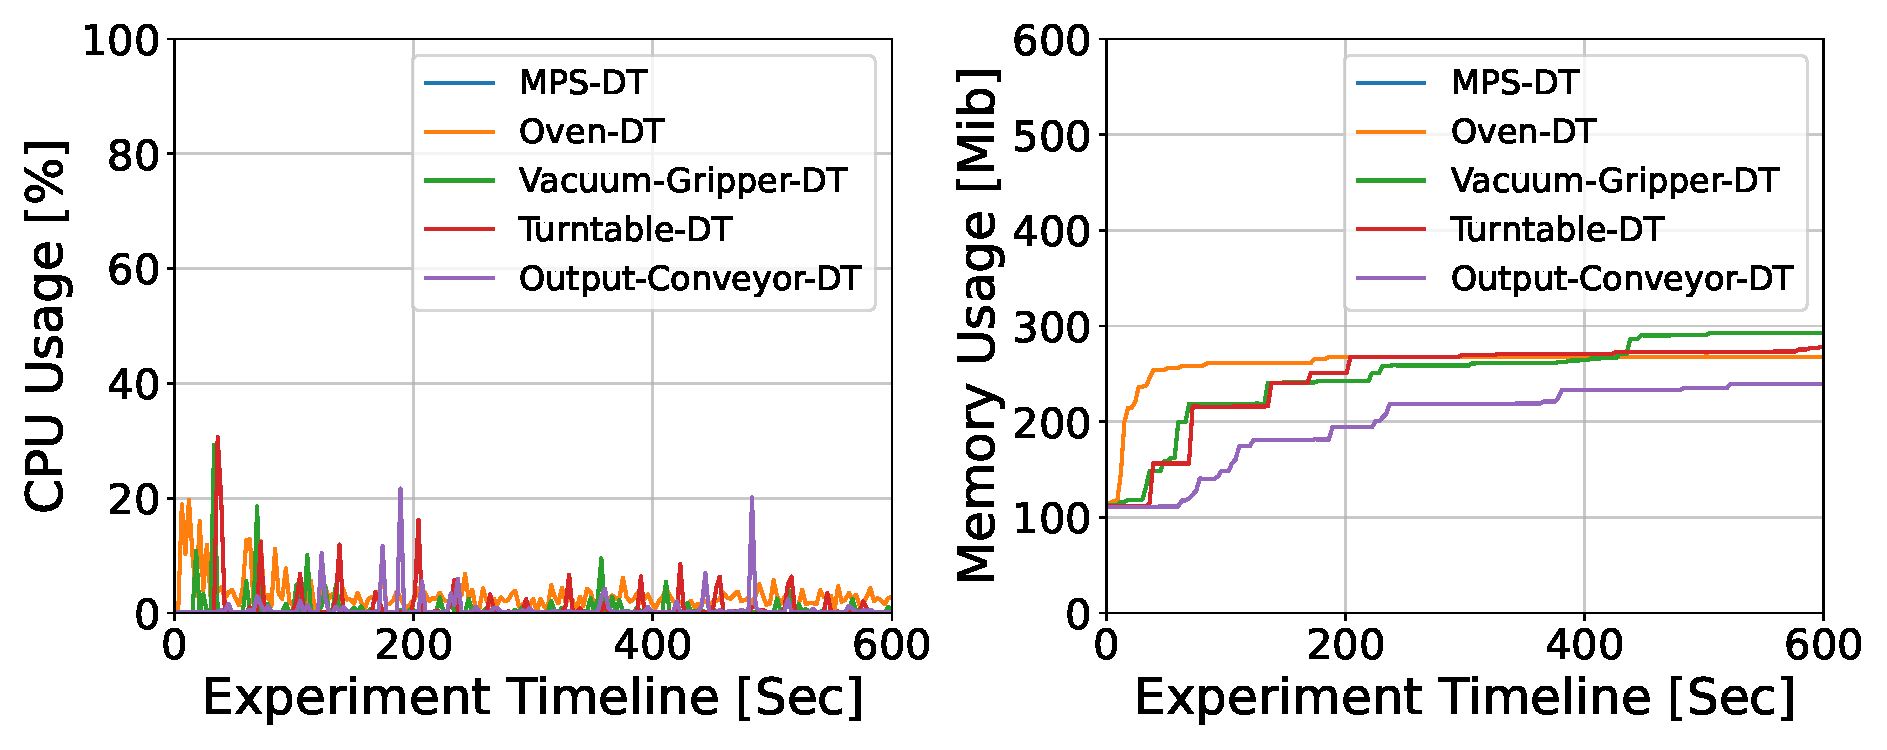
\includegraphics[width=\linewidth]{figures/wldt-results-2.pdf}\\[-2pt]
        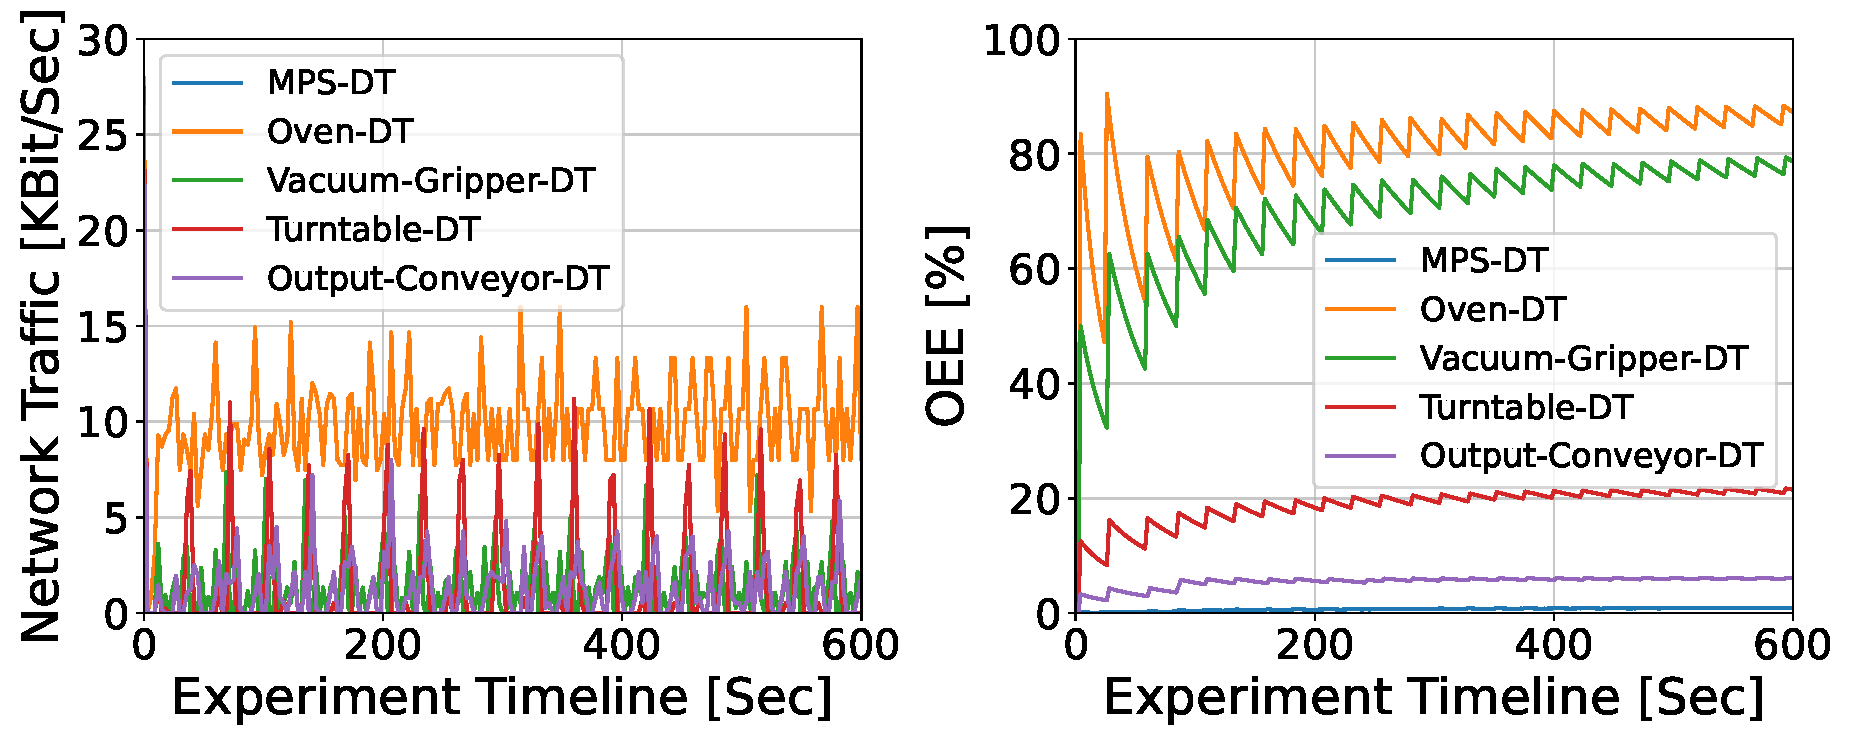
\includegraphics[width=\linewidth]{figures/wldt-results-1.pdf}
    \end{subfigure}
    \caption{Performance indicators of the Multiprocess Station DTs: CPU usage percentage [\%], Memory usage [Mib], Network usage [KBit/sec] and OEE [\%]}
    \label{fig:exp-results}
\end{figure}


To validate the \ac{WLDT} framework,
the \acp{DT} for the Multiprocess Station with Oven were containerized using Docker, and deployed on an Edge node with an Intel i7 2.4GHz processor and 32 GB of RAM.
%
Three key metrics for each DT for a total of 10 minutes (600 seconds):
\begin{itemize}
    \item \textbf{CPU Usage}: the percentage of CPU resources utilized by each DT instance over time;
    \item \textbf{Memory Consumption}: the amount of memory (in MiB) used by each DT instance during its operation;
    \item \textbf{Network Traffic}: the cumulative inbound and outbound network traffic (in Kbit/sec) generated by each DT instance.
    \item \textbf{OEE Computation}: the Overall Equipment Effectiveness calculated by each DT to assess machine and station performance.
\end{itemize}

\Cref{fig:exp-results} shows the results.
Analyzing CPU usage, there were no significant spikes during the production cycle.
Even during the most computationally demanding moments, CPU utilization remained around 30\%, indicating a stable and efficient execution.
%
The memory usage chart shows a similarly stable pattern, with DT instances settling around an average usage of 300 MiB, demonstrating consistent memory behavior over time.
As for network traffic, values remained low—typically around a few tens of Kbit/sec.
Noticeable traffic peaks correspond to active processing phases, where machines and their respective DTs exchange larger volumes of data.
%
Finally, the OEE graph highlights the performance of industrial machines computed by each DT. The Oven, which is the first machine in the station and requires the longest processing time, shows the highest OEE, as it remains under constant workload.
%
Conversely, the output conveyor exhibits a lower OEE, as it receives fewer parts to process due to the upstream bottleneck created by the Oven.

This experimental setup aimed to demonstrate the effectiveness of \ac{WLDT}-based DTs in an industrial setting.
The collected metrics confirm that DT instances can operate efficiently on standard commercial Edge nodes, handling CPU, memory, and network constraints while also supporting domain-specific computations such as OEE.
These results validate the potential of the \ac{WLDT} framework for practical DT development and deployment in real-world industrial scenarios.

%-------------------------------------------------
\subsection{Implementing Augmented Digital Twins}
%-------------------------------------------------

\begin{figure}
    \centering
    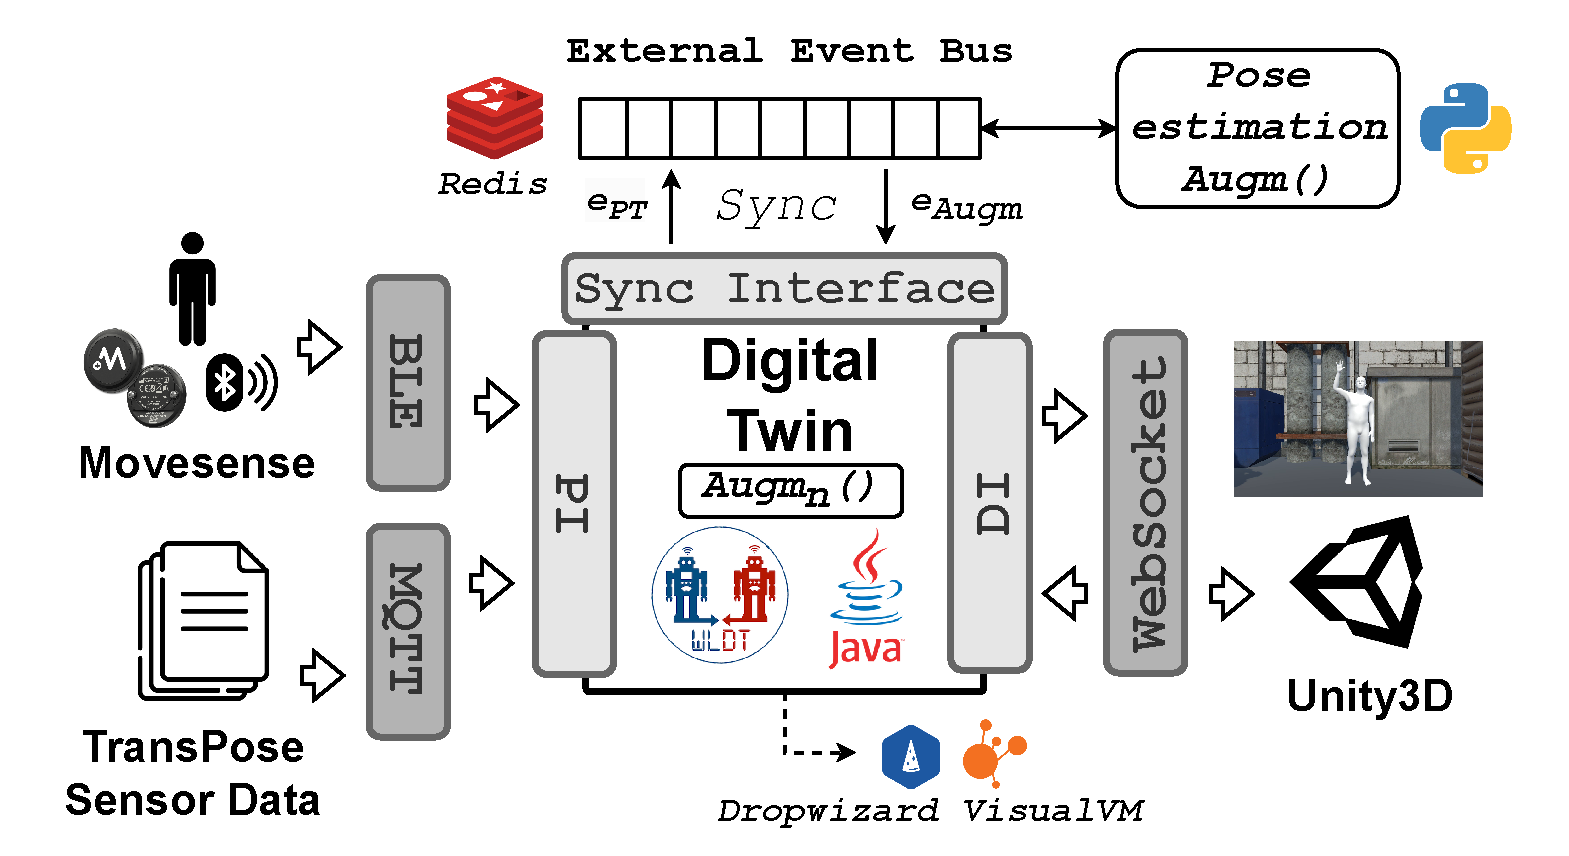
\includegraphics[width=0.9\textwidth]{figures/experimental_evaluation_scheme_new_industry.pdf}
    \caption{Experimental setup for evaluating the design of augmented digital twins for a pose estimation task.}
    \label{fig:augmentation-experimental-setup}
\end{figure}

A different experimental evaluation was conducted to validate the benefits of the modular design of augmentation proposed in \Cref{sec:dte:engineering-dt:dt-augmentation}.
%
The reference scenario involves the real-time monitoring of an industrial operator's movements within a manufacturing environment through a \ac{DT} whose state is augmented with pose estimation capabilities computed from inertial sensor data.

\Cref{fig:augmentation-experimental-setup} illustrates the experimental setup designed to evaluate the proposed augmentation function patterns within a \ac{DT}.
%
The \ac{DT} uses both physical devices and emulated traces, and embeds a machine learning model to estimate pose of the operator which is then visualized in a Unity3D\footnote{Unity: \url{https://unity.com/}} environment connected to the \ac{DT}.
%
This setup showcases how internal and external augmentation functions can be implemented in practice and what are the implications on the \ac{DT} performance.

The \ac{DT} acquires data from a Movesense Active sensor\footnote{Movesense: \url{https://www.movesense.com/movesense-active/}}: a wearable device featuring a 9-axis Inertial Measurement Unit (IMU) with accelerometer, gyroscope, and magnetometer capabilities, along with ECG and heart rate monitoring. This sensor, connected via Bluetooth Low Energy (BLE), allows for continuous tracking of physiological and motion-related data essential to represent the operator's state. Since the sensor can be configured to measure and send data with different sampling rates (13 Hz, 52 Hz, and 104 Hz) it was possible to test the \ac{DT} responsiveness under different conditions. 
%
For the reported experiments, the \ac{DT} has been deployed on a machine with an Intel i5-13600KF processor (5.1 GHz, 14 cores, 20 threads) and 32 GB of RAM and an RTX 4070ti GPU (12 GB GDDR6X).

%....................................................................
\subsubsection{Performance of Internal Augmentation Functions}
%....................................................................

To evaluate the performance of the augmentation functions, execution times, CPU usage, and memory consumption on the workstation were monitored.
%
Execution times were measured by testing various configurations.
The augmentation functions are implemented \emph{internally} in Java as periodic functions activated at a fixed period.
Each function computes the average of accelerometer values received from the Movesense sensor since the last activation.

In the first experiment, the activation interval of the functions was fixed (5 seconds).
Measurements of function execution time were taken using different sensor sampling frequencies (13, 52, and 104Hz) while varying the number of concurrently running functions (1, 3, and 5 functions).
%
\Cref{tab:AF_exec_time_fixed_act_period} presents the results from this experiment.
%
\begin{table}

    \centering
    \begin{tabular}{p{4cm} p{2cm} p{2cm} p{2cm}}
    \hline
    \textbf{\#Augm.} & \textbf{13Hz} & \textbf{52Hz} & \textbf{104Hz} \\ \hline
    \textit{1 function} & 2.55ms & 6.58ms & 10.76ms \\ \hline
    \textit{3 functions} & 2.69ms & 6.54ms & 8.42ms \\ \hline
    \textit{5 functions} & 2.79ms & 6.79ms & 11.79ms \\ \hline\hline
    \end{tabular}
    \caption{Average AF execution time with fixed activation period (5s) varying sensor sampling frequency and number of simultaneous functions.}
    \label{tab:AF_exec_time_fixed_act_period}
\end{table}
%
The experimental evaluation of augmentation functions confirmed that even when multiple augmentation functions coexist within the same DT instance the \ac{DT} maintains good performance.

In the second experiment, the sampling frequency was fixed at 13 Hz.
%
In this setup, both the number of functions and their activation intervals were varied (1, 5, 10, and 30 seconds). The results from this experiment are detailed in \Cref{tab:AF_exec_time_fixed_sens_frequency}.
The \ac{DT} performance is still robust, with minimal increases in execution times even as the number of functions and activation intervals varied. This confirmed the system ability to handle multiple augmentation functions efficiently.
%
\begin{table}
    \centering
    \begin{tabular}{p{4cm} p{0.4cm} p{2cm} p{2cm} p{2cm} p{2cm}}
    \hline
    \textbf{\#Augm} & \multicolumn{1}{c}{\textbf{1s}} & \multicolumn{1}{c}{\textbf{5s}} & \multicolumn{1}{c}{\textbf{10s}} & \multicolumn{1}{c}{\textbf{30s}}\\ \hline
    \textit{1 function} & \multicolumn{1}{c}{1.70ms} & \multicolumn{1}{c}{2.05ms} & \multicolumn{1}{c}{4.17ms} & \multicolumn{1}{c}{12.64ms}\\ \hline
    \textit{3 functions} & \multicolumn{1}{c}{1.57ms} & \multicolumn{1}{c}{2.15ms} & \multicolumn{1}{c}{3.54ms} & \multicolumn{1}{c}{13.92ms}\\ \hline
    \textit{5 functions} & \multicolumn{1}{c}{2.37ms} & \multicolumn{1}{c}{2.20ms} & \multicolumn{1}{c}{5.93ms} & \multicolumn{1}{c}{11.1ms}\\ \hline\hline
    \end{tabular}
     \caption{Avg AF execution with fixed frequency at 13Hz varying number of functions and activation period.}
    \label{tab:AF_exec_time_fixed_sens_frequency}
\end{table}

A third experiment was conducted to further examine execution times with up to five Movesense sensors connected to the DT simultaneously. The function activation frequency was fixed at 5 seconds, while the number of connected devices and sampling frequencies were adjusted. \Cref{tab:AF_exec_time_multiple_devices} summarizes the outcomes. 

\begin{table}
    \centering
    \begin{tabular}{p{4cm} p{2cm} p{2cm} p{2cm}}
    \hline
    \textbf{\#Devices} & \textbf{13Hz} & \textbf{52Hz} & \textbf{104Hz} \\ \hline
    \textit{1 Device} & 3.60ms & 16.29ms & 32.59ms \\ \hline
    \textit{3 Devices} & 7.70ms & 46.61ms & 81.76ms \\ \hline
    \textit{4 Devices} & 18.56ms & 62.06ms & 111.71ms \\ \hline
    \textit{5 Devices} & 23.12ms & 75.68ms & 104.42ms \\ \hline\hline
    \end{tabular}
    \caption{Average AF execution time with multiple devices connected, varying sensor sampling frequency.}
    \label{tab:AF_exec_time_multiple_devices}
\end{table}

To evaluate the resource consumption of the augmentation functions running on the DT, a fourth experiment was performed using a single augmentation function with a 5-second activation interval.
In this setup, both CPU usage (as a percentage) and memory consumption (in MB) were measured across the three different sampling frequencies available with Movesense sensor (13, 52 and 104Hz).
%
The results for CPU and memory usage are summarized in \Cref{tab:AF_CPU_MEM_usage}. 
%
\begin{table}[t]
    \setlength{\belowcaptionskip}{-6pt}
    \centering
    \begin{tabular}{p{4cm} p{3cm} p{3cm}}
    \hline
    \textbf{Data Freq.} & \textbf{CPU\%} & \textbf{Mem [MB]} \\ \hline
    \textit{13Hz} & 0.72\% & 158MB \\ \hline
    \textit{52Hz} & 0.98\% & 157MB \\ \hline
    \textit{104Hz} & 1.16\% & 156MB \\ \hline\hline
    \end{tabular}
    \caption{Average AF CPU and memory usage with one function at a 5-second activation period and varying sensor sampling frequency.}
    \label{tab:AF_CPU_MEM_usage}
\end{table}
%
The results showed that the DT maintained efficient resource utilization across different sampling frequencies, further validating the architecture ability to support high-frequency data streams and complex computations even with multiple data sources and physical devices connected and managed by the \ac{DT}. These experiments collectively demonstrated that the feasibility of the proposed event-driven architecture for DT augmentation functions.

The architecture successfully supports augmentation of DT functionalities, providing timely insights and maintaining good performance, even under varied and demanding conditions.


\subsubsection{Pose Estimation with External Augmentation}

\begin{figure}
    \centering
    \begin{subfigure}{0.49\textwidth}
    \centering
        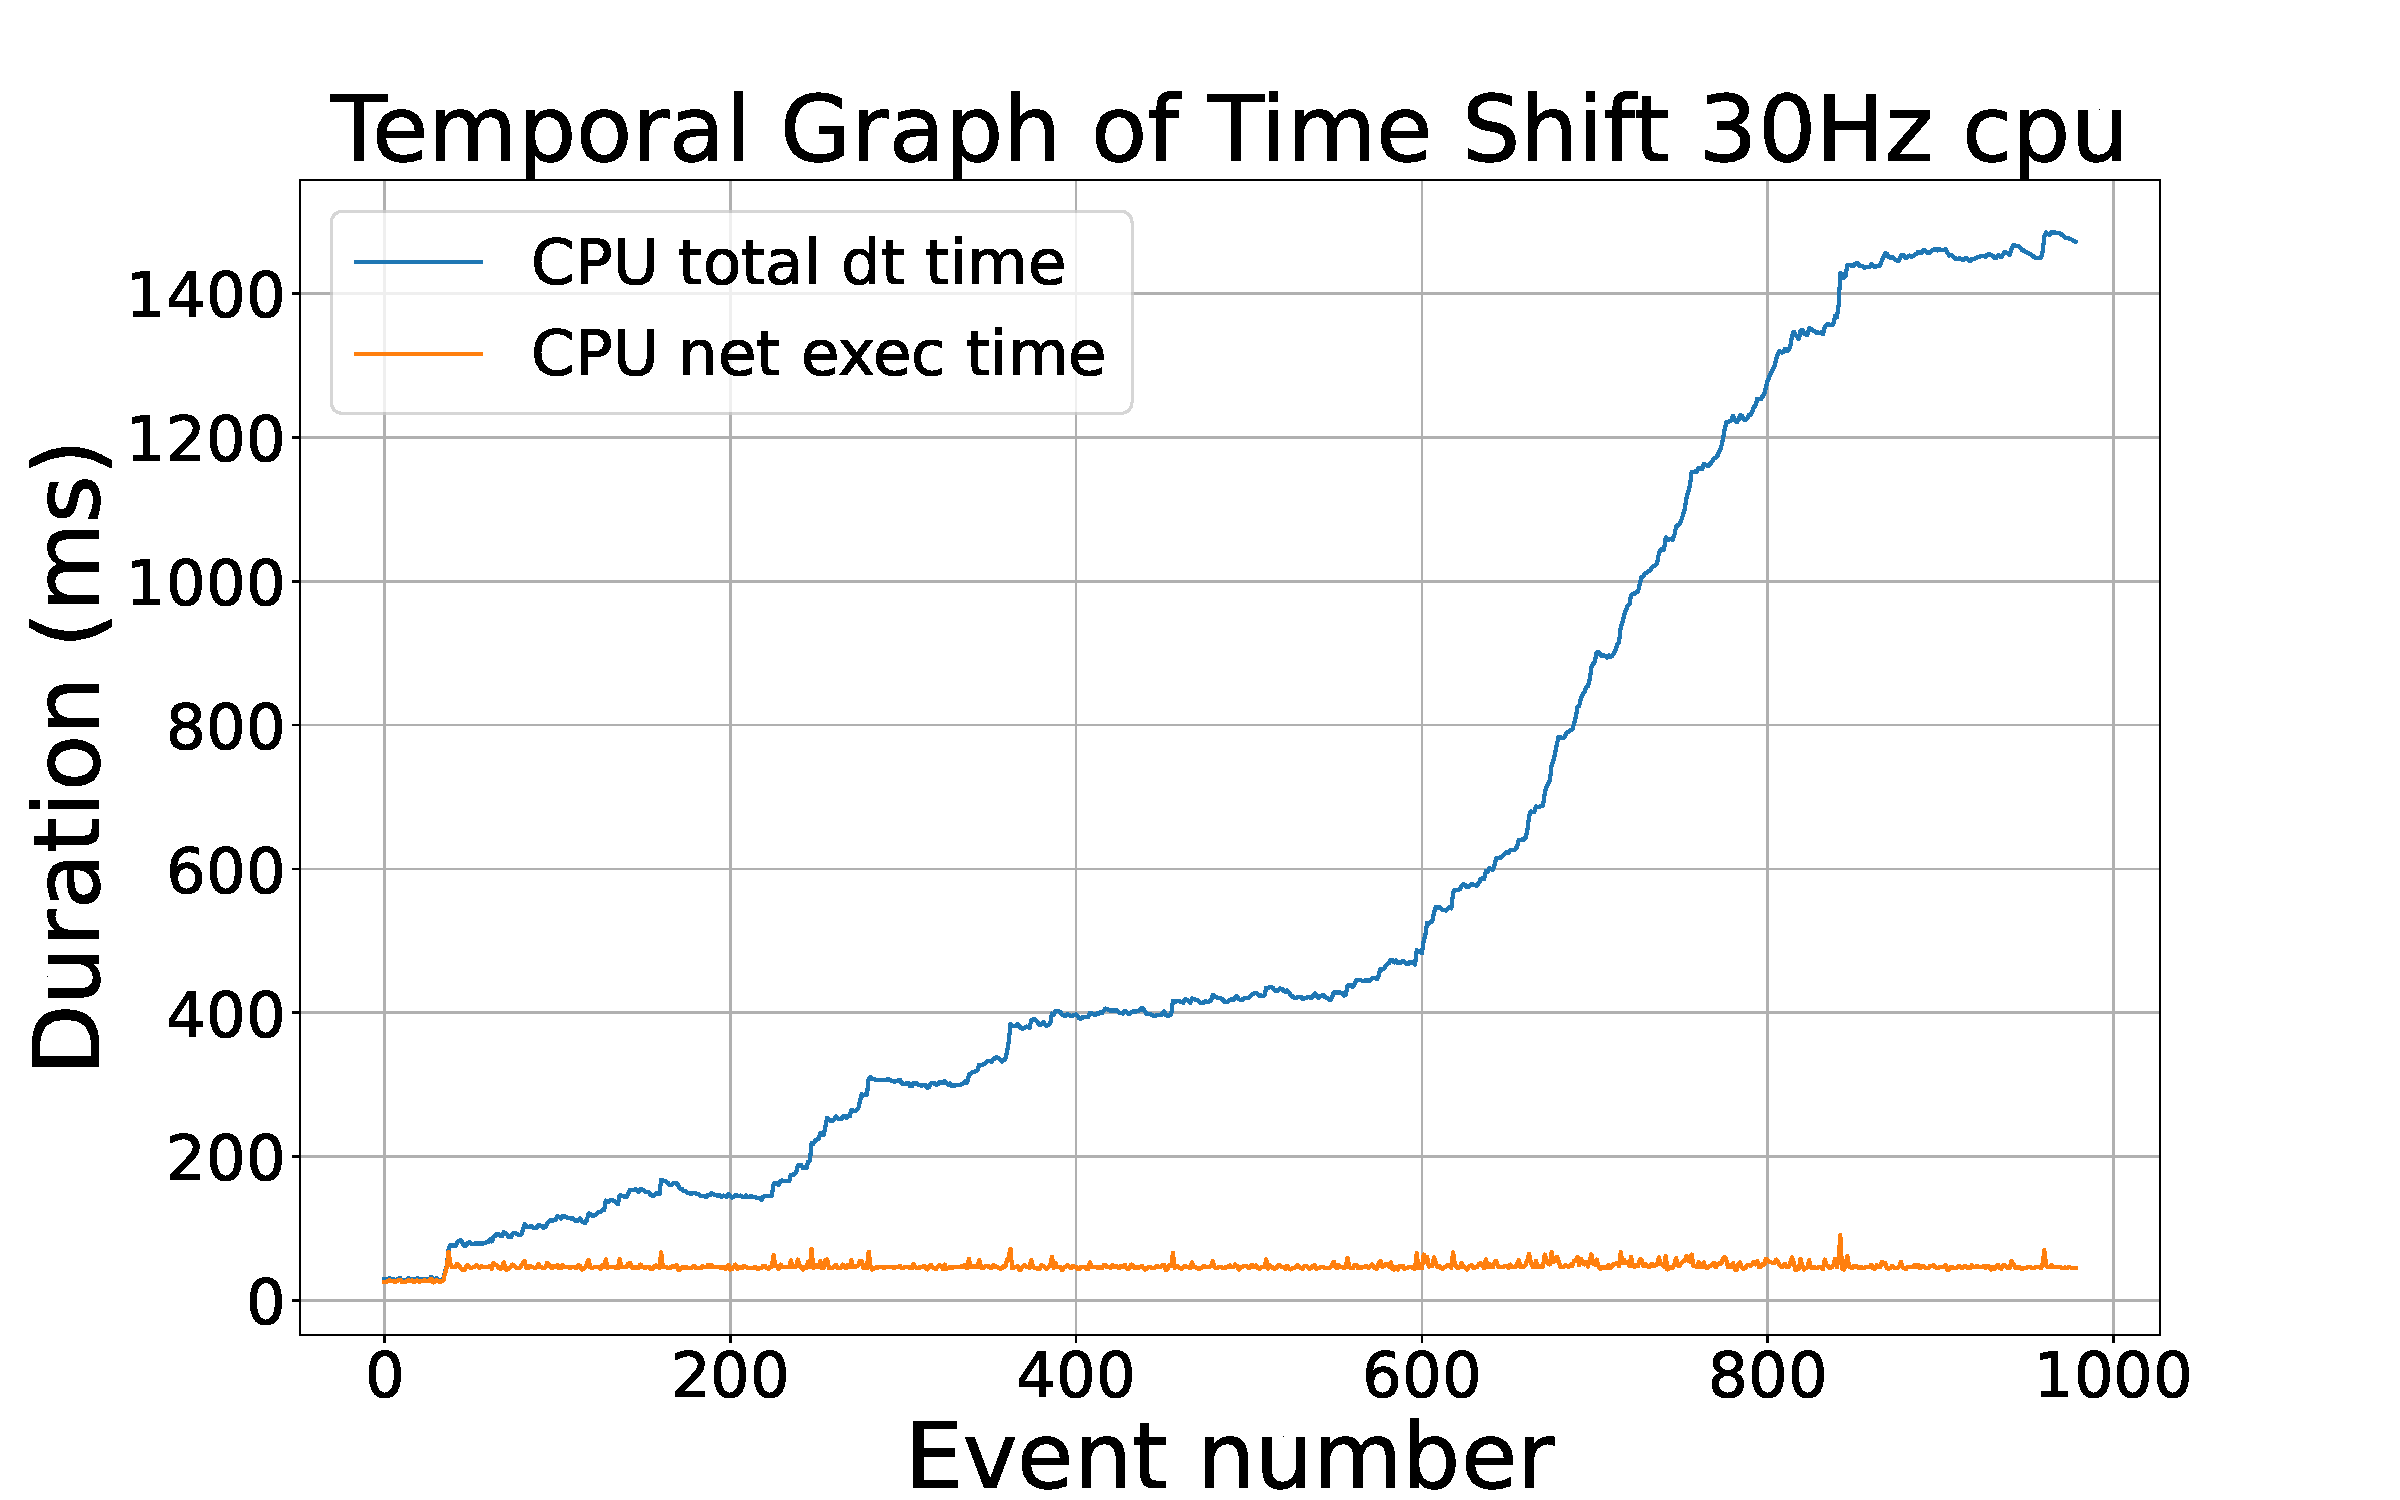
\includegraphics[width=\textwidth]{figures/temporal_graph_time_shift_30hz_cpu.pdf}
        \subcaption{}
        \label{fig:af_time_shift_30hz_cpu}
    \end{subfigure}
    \hfill
    \begin{subfigure}{0.49\textwidth}
    \centering
        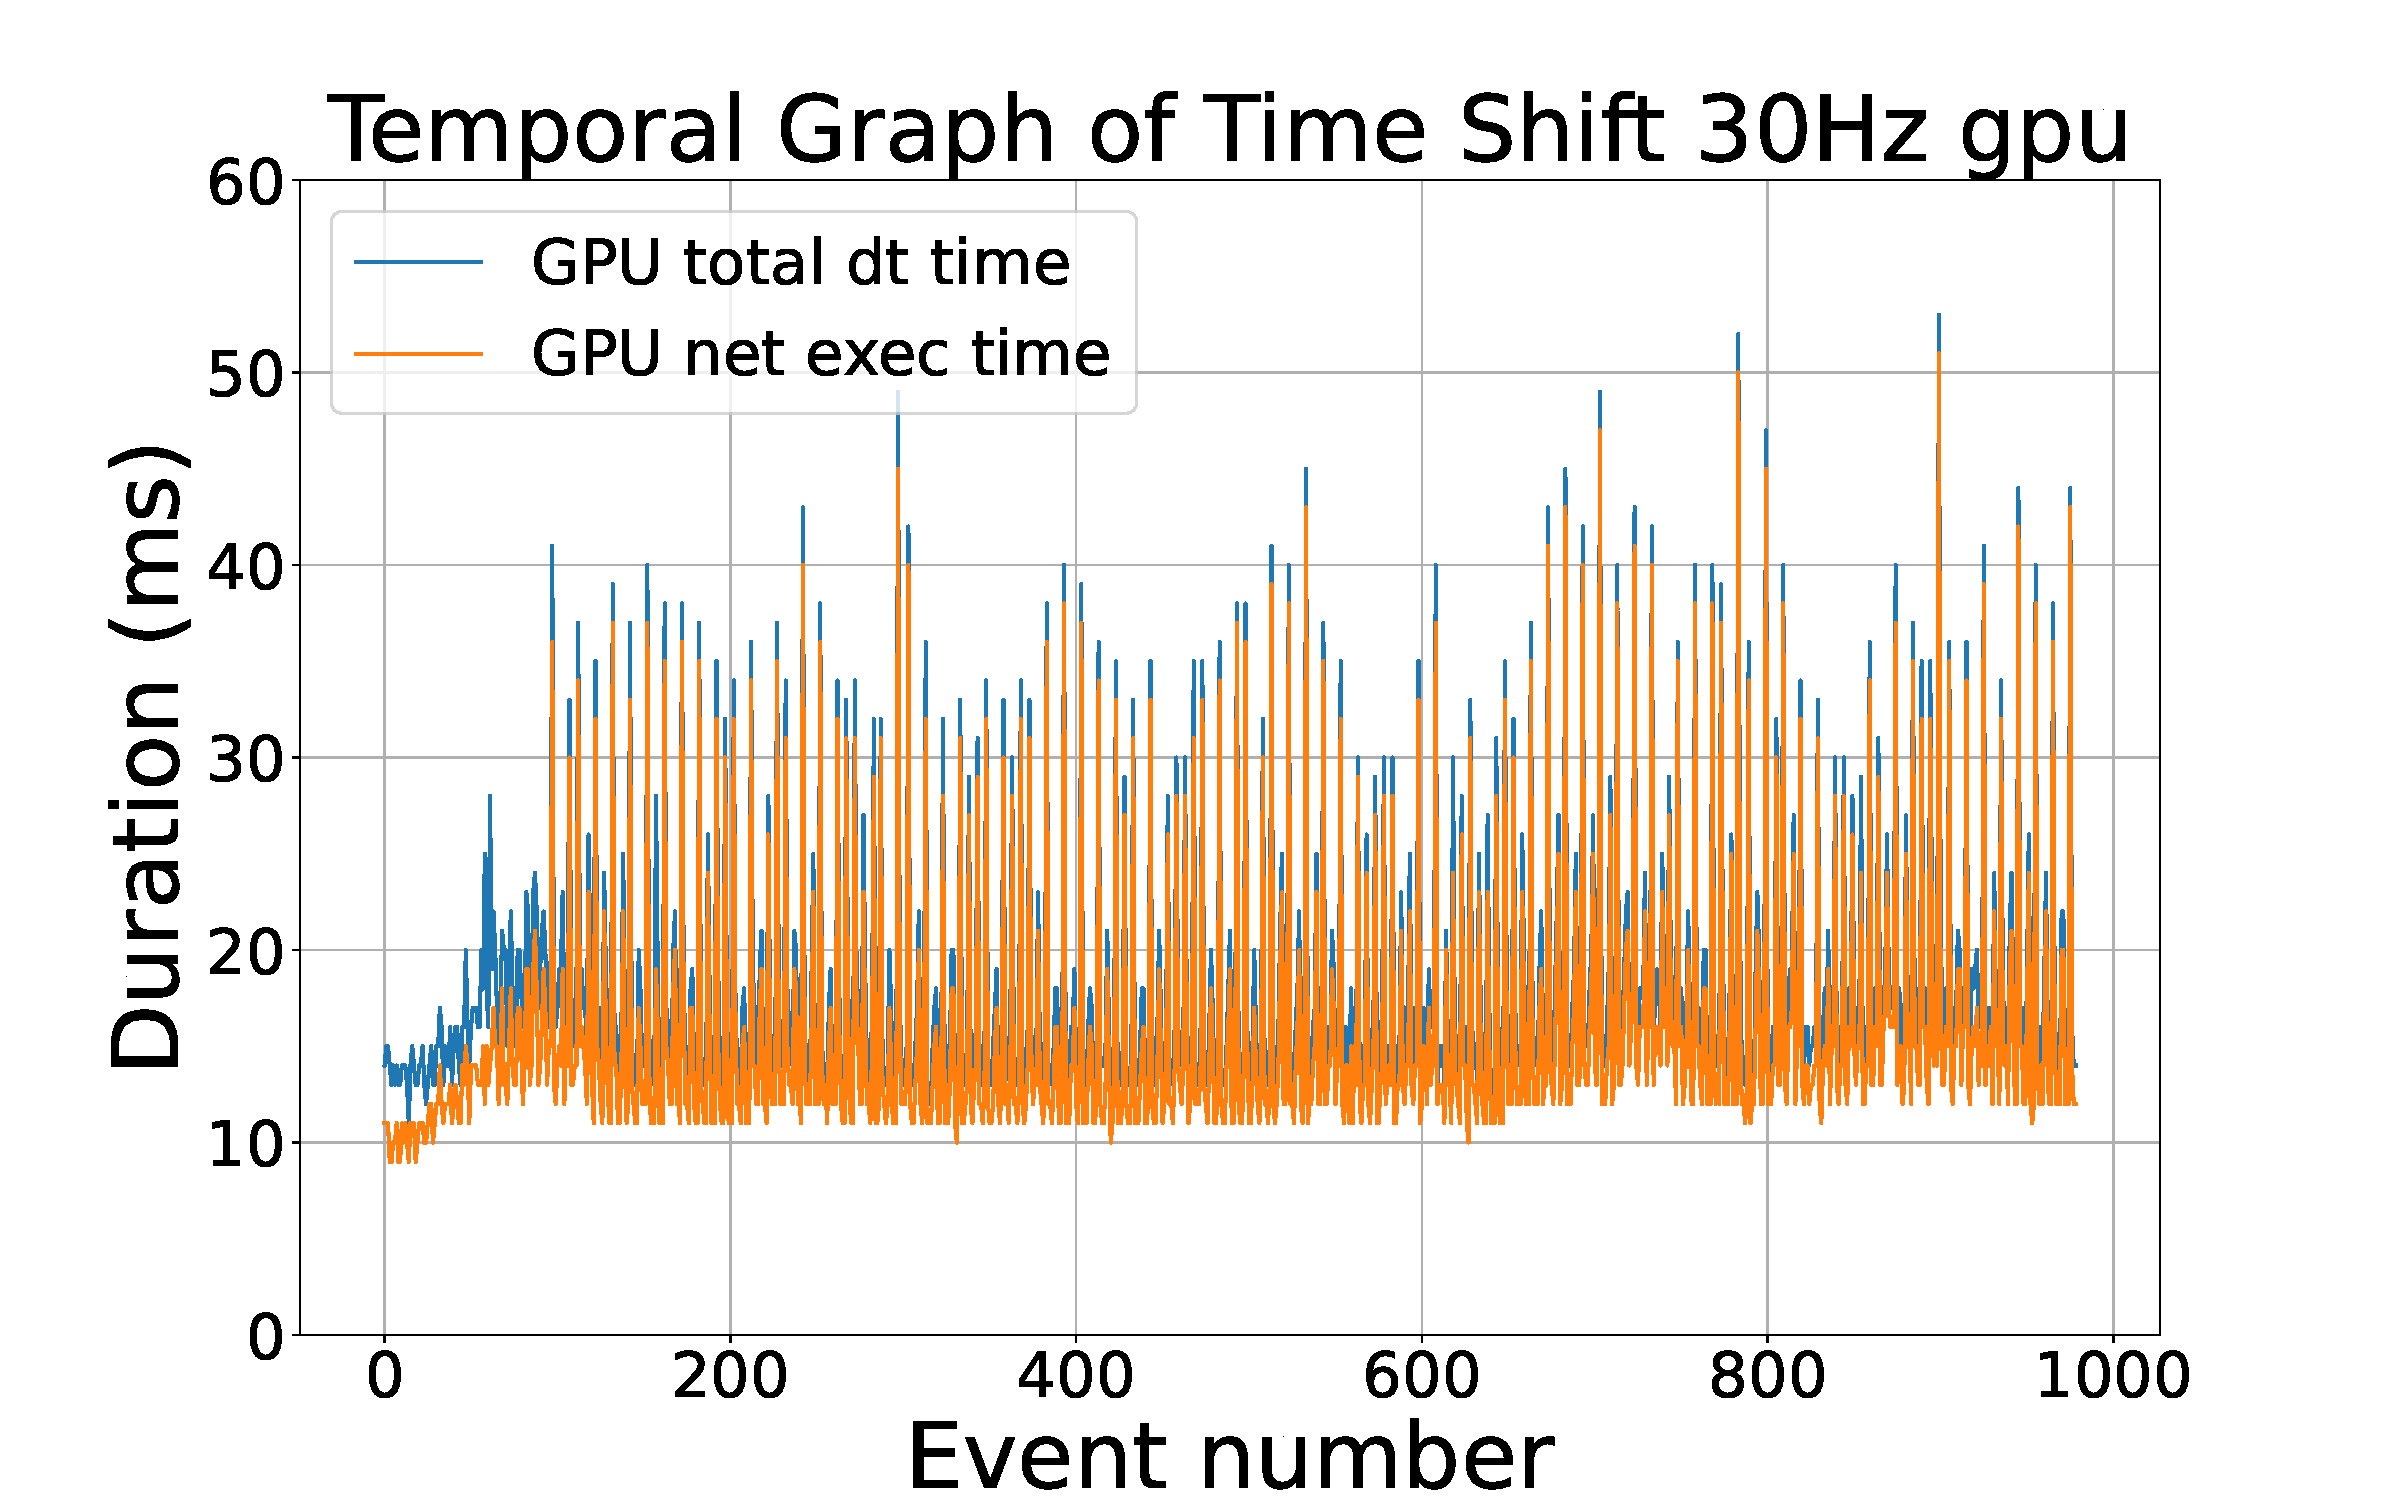
\includegraphics[width=\textwidth]{figures/temporal_graph_time_shift_30hz_gpu.pdf}
        \subcaption{}
        \label{fig:af_time_shift_30hz_gpu}
    \end{subfigure}
    \caption{Pose estimation latency computed within the DT compared to standalone execution, using the CPU (a) and using the GPU (b).}
    \label{fig:af_results}
\end{figure}

For the implementation of the pose estimation \ac{DT} feature,
the augmentation function is implemented externally using a Recurrent Neural Network from the TransPose project~\cite{TransPoseSIGGRAPH2021} using accelerometer data from six inertial sensors positioned on the operator's body to compute its position.
%
As shown in \Cref{fig:augmentation-experimental-setup} the original dataset of the project is used to emulate traces that are sent with a 30Hz frequency to the \ac{DT} through its physical interface using MQTT.
%
The augmentation function operates externally, running in parallel with the DT. Data exchange occurs via a Redis event bus, and once the position is determined, the \ac{DT} shadowing function publishes the result through the digital interface using a WebSocket to apply the inferred pose on a 3D model of a person in a Unity3D environment for visualization purposes.

The latency between data transmission and the reception of the estimated pose by the Unity3D application is measured to assess the performance of the external augmentation function.
%
First the neural network is executed using only the CPU, and then with GPU acceleration, to evaluate the impact of consciously allocating resources to augmentation functions.

Both the neural network model and the DT are executed on the same workstation. \Cref{fig:af_time_shift_30hz_cpu} illustrates the total latency introduced by the DT and the model compared with the latency associated to the same function executed outside the DT.
%
With CPU-only execution, the overall delay increases as the model cannot keep up, causing event queue buildup and increased latency. 
As shown in \Cref{fig:af_time_shift_30hz_gpu}, with the allocation of GPU resources the delay between transmission and reception remains stable over time, with most latency now attributed to model execution rather than DT processes.

This experiment demonstrates that the proposed model for the augmentation functions effectively supports developers in distributing the computational load on dedicated resources, thus improving the overall \ac{DT} performances. 

In conclusion, the experimental evaluation demonstrates that the proposed event-driven architecture for DT augmentation functions is both feasible and efficient.
The internal, external, and hybrid augmentation strategies offer flexibility, enabling real-time data processing and complex computations.
The architecture supports high-frequency data streams and provides timely insights, making it suitable for different applications.


%==============================
\section{Final Remarks}
%==============================

This chapter presents contributions to the engineering of \acp{DT} focusing on key challenges in the modeling and implementation of \acp{DT} as active components in an \ac{IoT} system, capable of integrating heterogeneous data sources, managing their synchronization with the \ac{PA} lifecycle and provide augmented functionalities. 

Despite the target scenario used for validation being an industrial manufacturing setting, emulated through a lab-scale production line, the proposed architectural framework and patterns are general and can be applied to other domains.
%
Indeed, the \ac{WLDT} framework, implementing the functionalities described in this chapter, has been used in different contexts such as smart-cities and healthcare. 

The chapter addresses the research question:

\paragraph{\ref{rq:1} How can we engineer \acp{DT} to integrate heterogeneous data sources and provide an up-to-date uniform representation of the mirrored assets?}
%
The modular architecture grounded on the concept of \acp{PhA} and \acp{DiA} effectively decouples the complexities of physical and digital environments from the core responsibilities of the \ac{DT}.
%
This enables integration of heterogeneous data sources by means of reusable components, simplifying the development of \acp{DT} and promoting interoperability.
%
Furthermore, the lifecycle management managed at the \ac{DT} level ensures that domain-specific synchronization requirements can be validated and enforced, providing applications with accurate and timely information about the state of the \ac{PA}.
%
Finally, the modular approach to \ac{DT} augmentation allows for the flexible integration of additional functionalities, either internally or externally, without impacting the core shadowing responsibilities of the \ac{DT}.


%%%%%%%%%%%%%%%%%%%%%%%%%%%%%%%%%%%%%%%%%%%%%%%%%%%%%%%%
\chapter{\aclp{DTE}}
\label{chap:dte:dte}
%%%%%%%%%%%%%%%%%%%%%%%%%%%%%%%%%%%%%%%%%%%%%%%%%%%%%%%%

%======================================================
\section{Characterizing \aclp{DTE}}
\label{sec:ecosystems}
%======================================================

As discussed in \Cref{sec:background}, the \ac{DT} concept is shifting from ultra-detailed replicas of individual \acp{PA} to contextualized models tailored to specific applications~\cite{minerva2020dtiot}.
%
However, many solutions either mirror isolated assets -- overlooking their interrelations -- or adopt monolithic models for complex systems (e.g., entire cities~\cite{Deren2021}).
%
In this paper, we focus instead on the idea of modeling such large-scale scenarios using what we informally define as a:

% \newtheorem*{dte}{Digital Twin Ecosystem}
% \begin{dte}
%     A dynamic set of \aclp{DT}, each representing a \ac{PA}, whose meaningful relationships within a target context make it valuable to consider their collective evolution to accurately reflect the mirrored portion of the physical world.
% \end{dte}

In order to characterize \acp{DTE}, in this section,
we analyze the challenges surfacing from the heterogeneity of complex domains (\ref{rq:dimensions})
and provide an operational definition of \acp{DTE} in terms of functionalities and services that consumers may expect to use (\ref{rq:functionalities}).
Finally, we compare architectural approaches for \acp{DTE} by investigating the state of the practice (\ref{rq:implementations}).


%=======================================================
\section{Operational Characterization}
\label{sec:operational-characterization}
%=======================================================

To better characterize the concept of \ac{DTE}, we analyze the fundamental functionalities to ease the fruition of services that span across several \acp{DT}.
%
We intend this operational definition to be general, regardless of the architectural design adopted to develop the ecosystem.

We consider the perspective of both \emph{managers} of the \ac{DTE} who need to oversee the creation and evolution of the ecosystem, and \emph{consumers} who instead are interested in exploiting the \ac{DTE} abstraction for their application goals.
%
We will then let these functionalities guide our implementation proposal that we describe in \Cref{sec:hwodt-idea}.

\subsubsection{Managing the \ac{DTE}}\label{sssec:operational-managing}

We define \ac{DTE} as a \emph{dynamic} set of \acp{DT} as members could join or leave the ecosystem at any time due for different reasons.
These include the \acp{PA} lifecycle (e.g., decommissioning) or application-specific inclusion criteria adopted when modeling the ecosystem (e.g., entering or exiting a geographical area).
%
To support this dynamism, \acp{DTE} should provide operations to \emph{add} and \emph{remove} \acp{DT}.
These can be public or restricted to administrators, and invocations can be either manual or automatically triggered by monitoring processes (or the \acp{DT} themselves) when detecting relevant changes in the physical environment.

A consequence of this dynamic management is the need to easily \emph{discover} which \acp{DT} are part of the ecosystem.
\acp{DTE} may hold an index of all (currently) registered \acp{DT}, each \emph{uniquely identified} and described with metadata to support fine-grained discovery.
%
A key piece of information to store is the mirrored \ac{PA} identifier, allowing tracking of both the digital and physical components of the ecosystem.
As noted in \Cref{ssec:dimensions}, since multiple \acp{DT} may represent the same \ac{PA} for different purposes, this information becomes especially valuable.
Moreover, to keep track of a \ac{DT} evolution, it should be possible to \emph{update} metadata over time.

\subsubsection{Exploiting the \ac{DTE}}\label{sssec:operational-exploiting}

\emph{Consumers} of a \acp{DTE} represent either human users, applications, or intelligent agents~\cite{burattini2025iot} which may be interested in observing the state of the registered \acp{DT} and exploiting their services.
%
An ecosystem should then offer functionalities to access individual \acp{DT} and ecosystem-wide services. 

This includes the ability to retrieve the current \emph{representation} of the state of all \acp{DT} and their relationship at a given time.
%
As the representation could grow very large, it can be more effectively managed by enabling consumers to \emph{query} the ecosystem, enabling them to select and aggregate relevant data across multiple \acp{DT}.
%
This supports the derivation of insights that would not be easily discovered by accessing each \ac{DT} individually.

Finally, given the dynamic nature of \acp{DT} continuously updating their representation of the corresponding \acp{PA}, \acp{DTE} should support \emph{observation} patterns -- even selectively through continuous queries~\cite{babu2001sigmod} -- to track changes of \acp{DT} and of the whole ecosystem over time.

Although not an operation provided by the ecosystem itself, we include \emph{navigation} by following \ac{DT} relationships as a fundamental feature of \acp{DTE} complementing the other interaction patterns.
%
This allows users to explore and discover information progressively.
Moreover, relationships may cross ecosystem boundaries, offering paths to discover related \acp{DTE}.

%=======================================================
\section{Architecting \aclp{DTE}}
\label{sec:architecting-dte}
%=======================================================

\begin{figure}[t]
    \centering
    \begin{subfigure}[b]{0.3\linewidth}
        \centering
        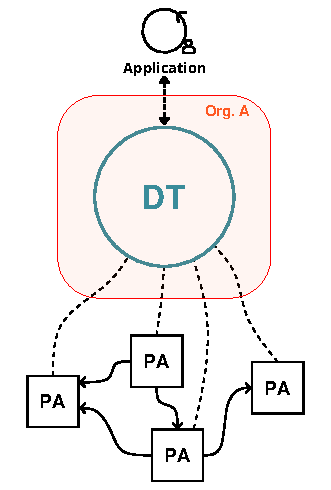
\includegraphics[width=\linewidth]{figures/hwodt/ecosystems_types-monolithic.pdf}
        \caption{\textbf{Monolithic} \ac{DTE}}
        \label{fig:ecosystem-monolithic}
    \end{subfigure}
    \hfill
    \begin{subfigure}[b]{0.3\linewidth}
        \centering
        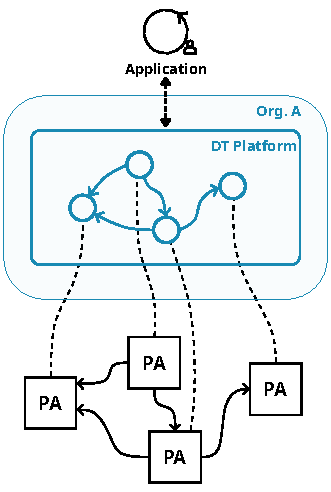
\includegraphics[width=\linewidth]{figures/hwodt/ecosystems_types-homogeneous.pdf}
        \caption{\textbf{Homogeneous} \ac{DTE}}
        \label{fig:ecosystem-homogeneous}
    \end{subfigure}
    \hfill
    \begin{subfigure}[b]{0.3\linewidth}
        \centering
        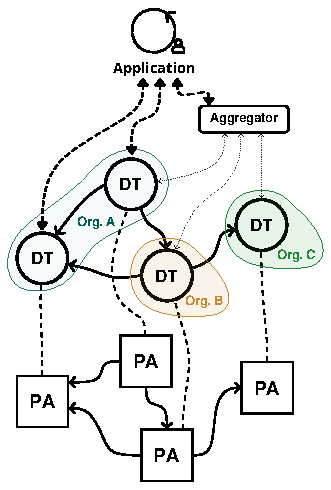
\includegraphics[width=\linewidth]{figures/hwodt/ecosystems_types-heterogeneous.pdf}
        \caption{\textbf{Heterogeneous} \ac{DTE}}
        \label{fig:ecosystem-heterogeneous}
    \end{subfigure}
    \caption{Three architectural approaches for \acp{DTE}: in \ref{fig:ecosystem-monolithic} a single \ac{DT} models the whole scenario; in \ref{fig:ecosystem-homogeneous} a single platform is used to build and deploy all the \acp{DT} in the ecosystem; in \ref{fig:ecosystem-heterogeneous} maximum flexibility is allowed, possibly reusing existing \acp{DT} under a common interface.}
    \label{fig:ecosystem-types}
\end{figure}

This section analyzes and compares approaches from current practice in applying \acp{DT} to complex scenarios involving multiple \acp{PA}.
We focus on four aspects derived from our \ac{DTE} characterization in terms of heterogeneity and operational behvior:
\begin{inlinelist}
\item the degree to which the ecosystem can evolve to reflect physical-world changes (\emph{evolvability}),
\item whether they support heterogeneous \acp{DT} within the same ecosystem (\emph{heterogeneity}),
and 
\item whether ecosystem-level functionalities are offered to users (\emph{services}).
\end{inlinelist}

We reviewed relevant works from the state of the art, survey papers, and technical documentation of \ac{DT} frameworks and platforms.
Although not a systematic review, our analysis shows three main emerging architectural approaches to implement \acp{DTE}.
%
We name these patterns \emph{monolithic}, \emph{homogeneous}, and \emph{heterogeneous} \acp{DTE}, and we schematically show their different architectures in \Cref{fig:ecosystem-types}.
We summarize our feature comparison in \Cref{tab:comparison-summary} and discuss the main peculiarities of each approach below.


\note{table}
% \noindent
% \begin{table}[t]
%     \centering
%     \begin{tabular}{l|c|c|c}
%     \toprule
%     \midrule
%     \textbf{} & \textbf{Mon.} & \textbf{Hom.} & \textbf{Het.} \\
%     \hline
%     \hline
%     \textit{Evolvability} & $\times$ & \checkmark & \checkmark
%     \\
%     \hline
%     \textit{Heterogeneity} & $\times$ & $\times$ & \checkmark
%     \\
%     \hline
%     \textit{Services} & \checkmark & \checkmark & \checkmark
%     \\
%     \hline
%     \bottomrule
%     \end{tabular}
%     \caption{Comparison summary of Monolithic (Mon.), Homogeneous (Hom.), and Heterogeneous (Het.) \acp{DTE} that shows supported (\checkmark)
%     %partially supported ($\sim$),
%     and not supported ($\times$) features.}
%     \label{tab:comparison-summary}
% \end{table}

\subsubsection{Monolithic \acl{DTE}}
\label{sssec:monolithic}

The most straightforward approach is to model the entire targeted context as a single, monolithic \ac{DT}.
Due to the fuzzy definition of a \ac{PA}, even complex entities (e.g., an entire city) can serve as valid physical counterparts of a single \ac{DT}, with some models explicitly capturing multiple internal components of such entities.

The main benefit of this approach is its simplicity in deriving the overall system architecture:
all physical-world data can flow into a single system built with a consistent technological stack (\Cref{fig:ecosystem-monolithic}).
%
A monolithic \ac{DT} also offers strong modeling capabilities and facilitates services such as running simulations on a single model of the entire ecosystem.

The drawbacks of the approach are on the management side. Representing with high fidelity dynamic scenarios involving multiple heterogeneous assets can be challenging, and even minor updates -- such as adding new entities or modifying the behavior of existing ones -- may require modifying the entire \ac{DT}.
%
This approach is not suited for rapidly evolving ecosystems or contexts involving multiple stakeholders.
%
Relying on a single \ac{DT} limits technological diversity and prevents the reuse of existing \acp{DT}, forcing the creation of a new, unified model.

Examples of monolithic \acp{DT} include modeling a single \ac{DT} for entire roads~\cite{KUSIC2023101858}, hospital buildings~\cite{dt_hospital}, or smart grids~\cite{9449682}. 

\subsubsection{Homogeneous \acl{DTE}}
\label{sssec:homogeneous}

We refer to \emph{homogeneous} \acp{DTE} when the approach relies on a general-purpose platform that natively supports the definition of multiple \acp{DT} (\Cref{fig:ecosystem-homogeneous}).
%
The \ac{DT} are hence homogeneous in their modeling and implementing technology as they are created within the same platform.
%
The native support for \acp{DTE} enhances adaptability to the evolving physical world as it is simple to add and remove \acp{DT} or update models.
%
Furthermore, the modeling and technological homogeneity make implementing ecosystem services relatively easy, as in the \emph{monolithic} approach.
%
Differently, though, it is possible to highlight the individuality of the involved \acp{DT}, which may independently process the relative data flows, offering better decomposition and separation of concerns.

However, the dependency on a single model and platform may introduce vendor lock-in, modeling and organizational constraints, limiting support for heterogeneous \acp{PA}.

An example of this approach is the Azure Digital Twins platform, which introduced the concept of a \emph{Twin Graph}\footnote{\url{https://learn.microsoft.com/en-us/azure/digital-twins/concepts-twins-graph}} to explicitly represent relationships among \acp{DT} modeled using a uniform \ac{DTDL}.


\subsubsection{Heterogeneous \acl{DTE}}
\label{sssec:heterogeneous}

The third approach is based on introducing a common interoperability layer on top of heterogeneous \acp{DT}.
%
By embracing the inherent heterogeneity of \acp{DTE}, it enables the reuse of existing \acp{DT} while ensuring uniform access and navigation for consumers (\Cref{fig:ecosystem-heterogeneous}).
%
\acp{DT} are implemented as standalone software components, each with specific models and technologies, and each exposing interfaces that can be used by applications directly or through intermediary aggregators.

This approach is well-suited for dynamic, open \acp{DTE} where \acp{DT} are developed by various stakeholders since the individual components are loosely coupled.
%
Furthermore, \acp{DT} are not limited to being part of only one ecosystem, granting an additional degree of flexibility.

To maintain interoperability, though, each \ac{DT} must be mapped to a shared metamodel to represent it within the ecosystem and expose a shared interface to enable seamless interaction.
This can lead to a potential loss of information and expressivity, as with any model conversion.
However, direct access to the original \ac{DT} remains possible when needing to use specialized services not easily mapped in the shared model.

Compared to previous approaches, where services are typically provided by the implementing technology/platform and benefit from modeling uniformity, implementing ecosystem-wide services in heterogeneous \acp{DTE} is inherently more complex.
%
This can be achieved through either fully distributed techniques
-- such as polystores~\cite{dggan2015polystore} or federated and link-traversal queries~\cite{schwarte2011semweb,quilitz2008querydistributed,bogaerts2021linktraversalquery} --
or by introducing a middleware (as shown in \Cref{fig:ecosystem-heterogeneous}) aggregating \acp{DT} and implementing the required functionalities.
%
This doubles as a way to set a clear boundary for operations, allowing a clear definition of which \acp{DT} belong to an ecosystem.

In this paper, we demonstrate how such an interoperability layer and ecosystem services can be implemented using Web technologies and standards, paving the way for the realization of open heterogeneous \acp{DTE}.

To make a parallel with open Web-based ecosystems, this would be similar to a web service exposing a well-documented public HTTP API, which does not prevent specialized consumers from using remote method invocation if they have specialized knowledge on how to interact with the server.

For the approach to be successful and encourage \ac{DT} developers to join heterogeneous ecosystems, the entry barrier needs to be set at a relatively low level to ensure take-up, while still maintaining a sufficient level of complexity to meet the overall objectives~\cite{kendall2021ndt}.



%%%%%%%%%%%%%%%%%%%%%%%%%%%%%%%%%%%%%%%%%%%%%%%%%%%%%%%%
\chapter{Operational Management of \aclp{DTE}}
\label{chap:dte:dtc}
%%%%%%%%%%%%%%%%%%%%%%%%%%%%%%%%%%%%%%%%%%%%%%%%%%%%%%%%

This chapter investigates \ref{rq:3} by exploring the challenges in the operational management of \acp{DTE} that involve the management of multiple \acp{DT} from a deployment and runtime perspective.
%
Several \acp{DT} need to be orchestrated on a cyber-physical computing infrastructure, ensuring that \acp{DT} are able to interact with the \acp{PA} they represent and maintain the target level of performance and synchronization. 
%
This problem is further exacerbated when considering that \ac{DTE} can involve \acp{DT} developed for different platforms, and computing infrastructures that span the whole \emph{edge-cloud continuum}. 

Motivated by these challenges, this chapter introduces the concept of a \emph{\ac{DTC}}, a middleware that aims to facilitate the operational management of \acp{DTE} by providing a unified interface to manage the deployment and runtime of \acp{DT} across heterogeneous \ac{DT} platforms and computing infrastructures.
%
This proposal complements the \ac{HWoDT} approach presented in Chapter~\ref{chap:dte:hwodt}, which focuses on the interaction with \ac{DTE}, rather than their operational management. 

The chapter analyzes the challenges in the operational management of \acp{DTE}, and presents a proposal for an architecture of the \ac{DTC} middleware. The functionalities are supported by a set of \emph{descriptions} that can inform the \ac{DTC} about the characteristics of the \acp{DT} and \acp{PA} involved in the \ac{DTE} and support stakeholders in having a clear understanding of the system state at any stage.


%=======================================================
\section{Operational Challenges}
%=======================================================

An orthogonal aspect of complexity when developing a \ac{DT} is understanding its non-functional requirements that allow for considering the \ac{DT} effectively synchronized.
%
The concept of \emph{entanglement}~\cite{dt-IoT-context-Minerva-2020} has been used to define the level of synchronization of the \ac{DT} with the \ac{PA} and can be measured with metrics that include network latency and computation time on both the physical device and the computing node that is running the \ac{DT}~\cite{bellavista2024odte}.

In recent years, with the increased availability of computing resources at the edge of the network, the concept of edge-cloud continuum has emerged as a paradigm to distribute computation across a variety of computing nodes, obtaining benefits in terms of latency and optimizing the overall workload of an \ac{IoT} system~\cite{Rosendo_Costan_Valduriez_Antoniu_2022}.
%
Like other \ac{IoT} system components, \acp{DT} can also be deployed within the continuum~\cite{Bellavista_Bicocchi_Fogli_Giannelli_Mamei_Picone_2024} with trade-offs in terms of entanglement, cost and resource availability.
%
The advantages of this approach, though, are offset by additional complexity in the operational management of the software system.
When it comes to \acp{DT}, this means choosing the suitable computing node to deploy the \ac{DT} software, to ensure the \ac{QoS} requirements are matched at runtime.
This can be challenging due to the cyber-physical nature of \acp{DT}.
Additionally, when several \acp{DT} are employed as parts of an ecosystem sharing the same computing infrastructure, it should be possible for operators to easily navigate the continuum and observe performance metrics to understand the potential impact of deploying new \acp{DT} in the system and eventually reconfigure it to balance the overall workload.

On the development side, the heterogeneity of \ac{DT} platforms poses additional challenges as they may constrain the ability to deploy a \ac{DT} across the edge-cloud continuum.
%
Indeed, while open-source platforms can be adapted to run on a generic infrastructure, proprietary ones are usually Platform as a Service solutions, bound to the cloud infrastructure. 
%
Developers tasked with implementing a \ac{DT} must hence evaluate the suitability of a given \ac{DT} platform, taking into consideration both the functional (i.e., meta-model, features, services) and non-functional (i.e., latency, computing power, privacy) requirements.

Since these requirements may vary significantly depending on the \ac{PA} being modeled it is realistic to assume that a complex \ac{DT}-based system may include \acp{DT} developed on different platforms.
%
This has surfaced challenges in the management of the development and deployment of \ac{DT}-based systems which may need to guarantee the \ac{QoS} requirements of \acp{DT} developed with heterogeneous technologies and platforms while managing a shared pool of heterogeneous computing resources.

The proposal of the \ac{DTC} aims to address the following goals:
\begin{itemize}
    \item \textbf{reducing deployment complexity} of a \ac{DT}-based system integrating \acp{DT} developed for different platforms sharing the same computing infrastructure.
    \item \textbf{facilitating the interaction of different stakeholders} with a \ac{DT}-based system enabling easy access of relevant information over the development-to-deployment lifecycle of \acp{DT}.
\end{itemize}

%========================================================
\section{Phases and Stakeholders}
%========================================================


The process of developing and managing a \ac{DTE} involves several critical phases, each essential for the effective development, discovery, selection, deployment, and operation of \acp{DT}.
%
These phases abstract the development-to-deployment lifecycle of \acp{DT} in a structured approach which is independent of the target application domain or specific technological choices.

Identifying these phases helps shape the requirements for the \ac{DTC} and understand the roles of the stakeholders that are involved in each phase.


\paragraph{DT Software Capabilities Discovery \& Selection}
As a starting point, every DT system is originating from the needs of a cyber-physical context.
%
This usually involves one or several \emph{\ac{PA} Owner} who are the stakeholders that possess the knowledge about the \acp{PA} and the goal that requires \acp{PA} to be modeled and digitalized~\cite{michael2024software}.
The \emph{\ac{PA} Owner} is also in charge of granting access to the \ac{PA} data and sensors. 
%
The first phase hence focuses on identifying DT capabilities that align with specific application and use case requirements.
%
This phase involves defining the functionalities of the DT, associating it with the corresponding physical asset category, specifying communication protocols, and detailing its properties, events, relationships, and available actions. 
%
Notably, an asset might have multiple owners.
For instance, an industrial machine is produced by a manufacturer and acquired by a company to employ it in one of its facilities.
The same machine is then owned simultaneously by the manufacturer who may have control of telemetry data and be interested in monitoring the machine to offer predictive maintenance services, by the company who might want to keep track of all the machines across facilities and by the facility manager who might monitor the state of operational of the machine in the specific production line it is employed. 
All the owners may have access to different data and model the same asset with different target goals.


\paragraph{DT Development and Platform Selection}

A \emph{\ac{PA} Owner} may commission the development of a \emph{DT Developer} to implement the DT for the PA. The developer will implement a DT using a target technological stack, that depends on their expertise and the availability of the computing infrastructure that is available for the deployment of the DT.
%
In this phase it is necessary to ensure that the chosen DT requirements can be effectively implemented on a specific platform.
%
This phase involves defining platform-specific configurations, including implementation details, required configuration parameters, and technical requirements.
%
Notably, the \emph{\ac{PA} Owner} is usually the (virtual) owner of the computing infrastructure on which the DT will be eventually deployed. When the DT is developed as commissioned by the \emph{\ac{PA} Owner} this may influence the technological choices of the \emph{\ac{DT} Developer}.
%
This doesn't always need to be the case though, it can be reasonably expected that in the near future \acp{DT} implementations for specific kinds of assets would be made available to owners of such assets either publicly or commercially.
These would be implemented either by manufacturers or a community of \emph{\ac{DT} Developers}.
Such reusable \acp{DT} would then be implemented with a given technological stack and need to be deployed on the available resources of the \emph{\ac{PA} Owners}, in order to be configured and connected to the locally available \acp{PA}. 
Similarly, such reusable \acp{DT} could be offered as-a-service and made available only as instances deployed on commercial platforms. This adds a further layer of complexity to the management of the computing infrastructure running the possibly different \acp{DT} in an organization.


\paragraph{Digital Twin Deployment}

Once a DT is developed (from scratch or reusing existing implementations) the next goal is to run it on a computing infrastructure.
This step involves a \emph{DT Operator} who have knowledge about the \ac{DT} requirements and can configure the computing infrastructure to make sure that the DT is deployed correctly and gets access to the \ac{PA} data streams (this can be the same person as the \emph{DT Developer} in a typical Dev-Ops fashion).
%
Deploying a DT can be a challenging task, involving several steps that depend on the complexity of the deployment infrastructure and the requirements of the DT.
%
This phase is crucial to ensuring that all deployment conditions are met, including 
the availability of deployable artifacts, and the correct setup of communication configurations, enabling interaction with both physical and digital entities.
%
In a computing continuum, a DT may need to be deployed at different levels either on the edge, fog or cloud depending on the admissible trade-offs between network latency and computing power requirements. Notably, \acp{DT} might need to be moved across this continuum for a variety of reasons, either being connectivity requirements with the \ac{PA} (and thus a DT may move horizontally in the continuum) or changes in synchronization requirements or scaling (and thus moving vertically in the continuum). Finally, the same \ac{PA} could be connected to different \acp{DT} replicas, serving different use cases~\cite{dt-IoT-context-Minerva-2020}.

\paragraph{Running Digital Twin}

The last phase starts once the \ac{DT} is up and running. In this phase the DT must be identified, described, and reachable by consumers.
%
This phase is critical for maintaining an accurate and up-to-date representation of the DT instance, managing its interaction protocols, handling lifecycle transitions, and enabling real-time state monitoring and interaction with the twin.
%
The ability to monitor information about running \acp{DT} is essential for ensuring synchronization with physical assets, supporting advanced digitalization processes, and facilitating interoperability within complex cyber-physical systems.


\begin{figure}
    \centering
    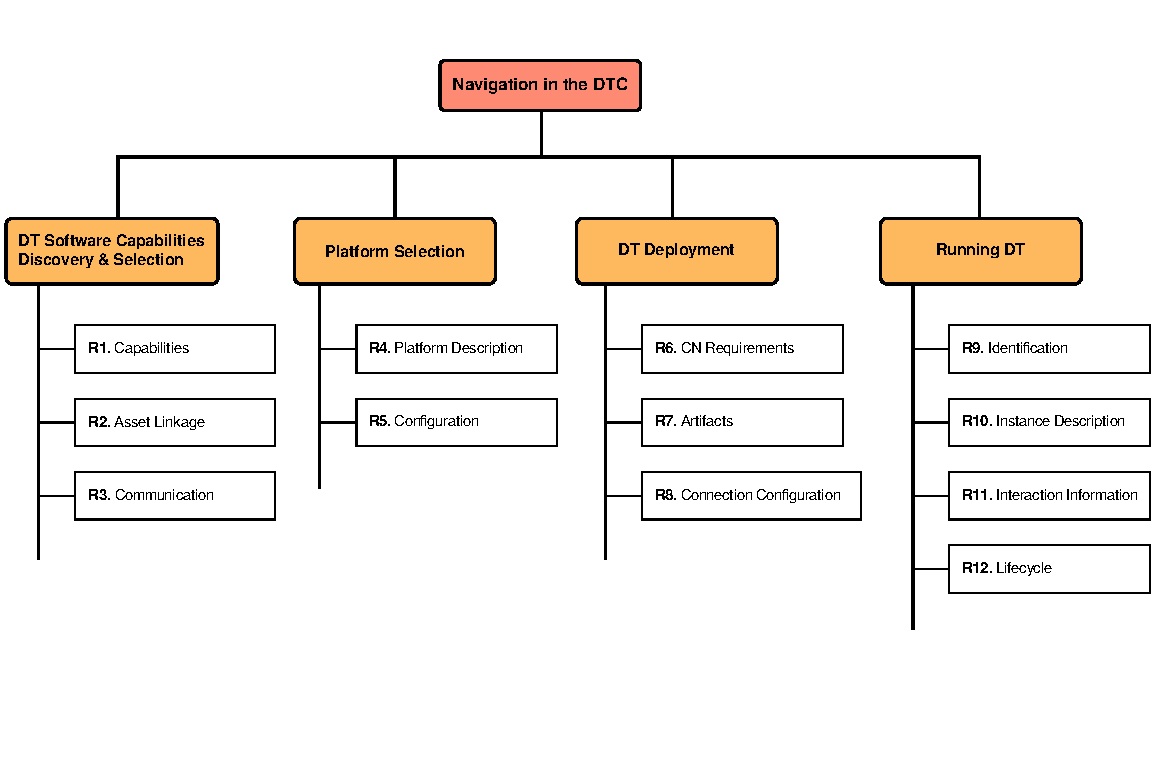
\includegraphics[width=0.9\textwidth]{figures/dtc/dtc-requirements.pdf}
    \caption{Phases and requirements for managing \acp{DT} in a \ac{DTC}.}
    \label{fig:dtc-requirements}
\end{figure}

\Cref{fig:dtc-requirements} summarizes the \emph{information} requirements for managing \acp{DT} across these phases, namely what kind of information is necessary to support stakeholders in each phase, and ensure that the phase can run successfully.
%
These requirements guide the design of \emph{descriptions} that can be used to inform the \ac{DTC} about the characteristics of the \acp{DT} to deploy and manage, in a platform-agnostic way.


%=======================================================
\section{Key Elements and Descriptions}
%=======================================================

To address the challenges in the operational management of \acp{DTE}, the \ac{DTC} relies on a set of key elements and their structured descriptions that provide a structured way to represent and manage the various components involved in a \ac{DTE}.

\begin{table}
    \centering
    \small
    \begin{tabular}{p{2cm} p{8.5cm} p{2cm}}
    \toprule
    \textbf{Entity} & \textbf{Description} & \textbf{Req.} \\
    \hline
    \textbf{Physical Asset Schema (PAS)} & Defines the abstract capabilities and interaction patterns of a specific type of industrial asset (e.g., robotic arm, conveyor system). Provides essential metadata for communication protocols, API definitions, and interface configurations without specifying instance-specific values like IP addresses or credentials. & R1, R2, R3 \\ \hline
    \textbf{Physical Asset Instance (PAI)} & Represents a deployed instance of an asset as defined by the PAS. Includes instance-specific configurations like network settings, authentication credentials, and protocol-specific settings. Facilitates the runtime communication between the DT and the physical asset. & R1, R2, R3 \\ \hline
    \textbf{Digital Twin Schema (DTS)} & Defines the capabilities, behaviors, and structural components of a Digital Twin, linking the digital representation to its corresponding physical asset. Specifies properties, events, relationships, actions, and fidelity between the physical and digital counterpart. & R1, R2, R3 \\ \hline
    \textbf{Digital Twin Package (DTP)} & Defines the platform-specific implementation of the DTS, including code, configuration parameters, and dependencies required for deployment. Ensures the fidelity and communication requirements of the DTS are met during deployment. & R6, R7, R8 \\ \hline
    \textbf{Digital Twin \-  Instance (DTI)} & Represents a running instance of the Digital Twin, including metadata for orchestration, monitoring, and lifecycle management. Tracks software lifecycle states and exposes relevant runtime metrics. Ensures the connection between the DTC and the deployed DT instance. & R9, R10, R11, R12 \\
    \hline
    \textbf{Runtime Platform (RP)} & Describes the underlying computing infrastructure and environment where the Digital Twin is deployed. This includes details about the hardware, software, and network configurations that support the DT's operation. & R4, R5 \\
    \bottomrule
    \end{tabular}
    \caption{Overview of DTC Entities: Characteristics, Responsibilities, and Associated Requirements}
    \label{table:dtc_descriptions_requirements}
\end{table}


At the core of this descriptive framework is the \textit{Physical Asset Schema} (PAS), which serves to uniquely define a specific \textit{type} of industrial asset---such as a robotic arm, conveyor system, or CNC machine.
%
The PAS encapsulates essential metadata that describes how assets of this category are expected to interact within a digital environment. This includes supported communication protocols (e.g., MQTT, OPC UA, HTTP), standardized API definitions, and more broadly, the configuration of interfaces and interaction models required for monitoring, control, and integration across systems. It is important to note that the PAS does not contain instance-specific values such as IP addresses, port numbers, or credentials. Instead, it provides a structured description of the expected capabilities and modes of interaction for devices of a given type.
%
This is similar to the concept of \emph{Thing Model} in the context of the \ac{WoT}~\cite{wot-td} which only focuses on capabilities and abstracts completely from protocols and implementation details. The PAS, instead, includes this information, as it is more closely related to the physical devices and not on their virtual \emph{Thing} representation. 

This schema is essential for the \ac{DTC} to understand how different \ac{PA} conform to specific interaction patterns and how to configure communication with them. 

Building upon the PAS, the \textit{Physical Asset Instance} (PAI) represents a deployed instance of an asset as defined by the PAS.
%
While the PAS defines the abstract capabilities and expected interaction patterns of a category of assets, the PAI provides the concrete, instance-specific configuration required for operational integration. This includes network information (such as IP addresses and ports), authentication credentials, and protocol-specific settings like MQTT topics or OPC UA node identifiers.
%
These configurations are essential to enable runtime communication between the DT and the physical asset, supporting dynamic discovery, secure interfacing. As such, the PAI forms the operational bridge that links the abstract asset description to real-world deployment contexts, ensuring that the DT can monitor and interact with its physical counterpart in a precise and reliable manner.
%
The \ac{WoT} \ac{TD} can be used for this scope as it includes the necessary information to describe how to connect to a specific device instance.

Following the same principles and responsibilities of the PAS, the \textit{Digital Twin Schema} (DTS) defines the capabilities and behaviors of a DT independently of any concrete implementation.
%
It establishes a reference to the corresponding \ac{PA} category, ensuring semantic linkage between the physical and digital representations. The schema outlines the structural components of the DT, such as its properties, observable events, defined relationships, and available actions. It also specifies the target \emph{fidelity} of the DT, capturing the mirrored functionalities of the physical counterpart within a given context and under specific application goals.

The \textit{Digital Twin Package} (DTP) represents instead the software implementation of a given schema on a target \ac{DT} platform.
%
The package includes all platform-specific implementation artifacts required for deployment and execution.
%
It incorporates the executable code, configuration parameters, and platform dependencies, ensuring compliance with the DTS's fidelity and communication requirements.
%
It also provides detailed bindings for the declared communication protocols---e.g., how MQTT is used to interface with physical assets and how HTTP APIs enable interaction with external digital services.

When a package is deployed within the DTC, it gives rise to a \textit{Digital Twin Instance} (DTI).
%
This instance represents the active, running version of the DT within the operational infrastructure and includes all metadata necessary for orchestration, monitoring, and software lifecycle management.
The DTI maintains references to its originating schema and the platform on which it is deployed, along with essential access information such as IP addresses, ports, and authentication tokens. It also exposes relevant runtime metrics—including CPU, memory, and network utilization—as well as any endpoints required to access its services and functionalities.
%
In addition, the DTI tracks and exposes the \ac{DT} connectivity information tracking whether the \ac{DT} is connected to the \ac{PA}. These lifecycle states pertain strictly to the operational status of the deployed software component and are independent of the internal logic or functional behavior of the DT itself (differently from the synchronization lifecycle discussed in \Cref{sec:dte:engineering-dt:dt-lifecycle}).
%
Functional state and domain-specific behavior remain under the responsibility of the DT and are communicated through its defined interfaces in the digital space (e.g., through the \ac{DTKG} if considering a \ac{HWoDT} ecosystem \Cref{chap:dte:hwodt})

With reference to the requirements identified in \Cref{fig:dtc-requirements}, \Cref{table:dtc_descriptions_requirements} summarizes the key elements and their associated responsibilities in supporting the operational management of \acp{DTE}.
%
The integration of the PAS, PAI, and DTS effectively addresses the core requirements \textbf{R1.Capabilities}, \textbf{R2.Asset Linkage}, and \textbf{R3.Communication}, which are focused on the representation of features of the \acp{PA} and \acp{DT}, the relationship that links a \ac{DT} to a specific \ac{PA}, and the necessary communication protocols.
%
These descriptions support the \emph{DT Software Capabilities Discovery \& Selection} phase, enabling stakeholders to explore available \acp{PA} and their corresponding DT types based on defined capabilities and interaction patterns.
%
Additionally, the DTP supports requirements \textbf{R6.Computing Node Requirements}, \textbf{R7.Artifacts}, and \textbf{R8.Connection Configuration}, which pertain to platform-specific aspects to support the creation of DT instances within the DTC and can hence support the \emph{Digital Twin Deployment} phase.

The DTI is responsible for addressing the requirements \textbf{R9.Identification}, \textbf{R10.Instance\- Description}, \textbf{R11.Interaction\- Information}, and \textbf{R12.Life\-cycle}, which in the \emph{Running Digital Twin} phase support stakeholders in the identification of the DT instance, the discovery of its status and interaction descriptions, as well as its connectivity with the \ac{PA} during operation.


\textbf{R4.Platform Description} and \textbf{R5.Configuration} are supported by the \textit{Runtime Platform} (RP) description.
%
Differently from the other descriptions, these are tied to the computing infrastructure and the target platforms on which the \ac{DT} can be deployed. 
%
\textbf{R4}, includes platform-dependent attributes such as the platform type, supported communication protocols, and data formats, enabling the DTC to match DTPs to the correct platform.
%
Additionally, \textbf{R5} plays a crucial role in establishing the necessary parameters and operational requirements specific to the platform and implementation. Proper configuration ensures that the DT functions optimally by aligning its settings with platform constraints, communication protocols, and performance expectations.  

Together, these components support stakeholders to seamlessly identify and discover managed \acp{PA}, understand their capabilities, and determine the availability of corresponding \ac{DT} packages for deployment. This structured approach ensures that the DTC facilitates efficient asset discovery, aligns with system interoperability needs, and supports dynamic integration across diverse environments. 

%=======================================================
\section{Architecture of the \acl{DTC}}
%=======================================================

\begin{figure}
    \centering
    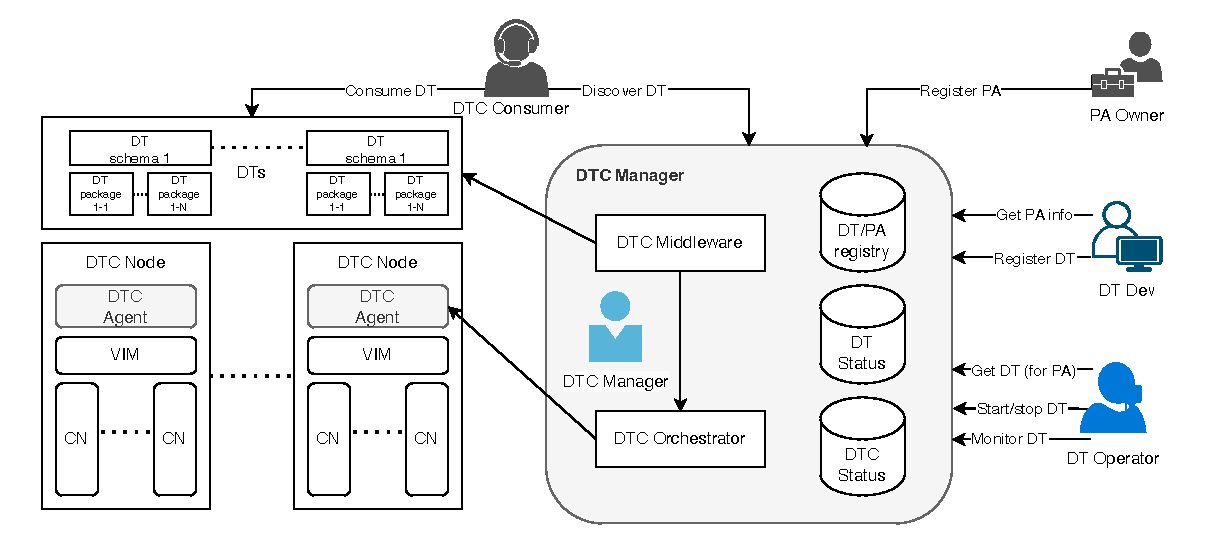
\includegraphics[width=\textwidth]{figures/dtc/architecture_new_v2.pdf}
    \caption{Functional Architecture of the \ac{DTC} with the main components and the interactions with stakeholders.}
    \label{fig:dtc-architecture}
\end{figure}

The aim of the DTC is to create a new open-system perspective of connected, interoperable and pervasive DTs modeled and engineered to create an effective cyber-physical abstraction layer.
%
This requires, first, facilitating the execution of DTs on a set of DT platforms.
Second, by exploiting the advantages of a broad compute continuum of cloud and edge resources, to deploy the DTs on the \textit{best} Compute Node (CN) available to guarantee application requirements.
%
The architecture of the DTC is depicted in \Cref{fig:dtc-architecture} and includes DTC functional blocks (grayed boxes), infrastructure modules, DT artifacts, while highlighting the interactions of DTC stakeholders. 

Other than the already introduced roles of \emph{PA Owner}, \emph{DT Developer}, and \emph{DT Operator}, we introduce the roles of \emph{DTC Manager} and \emph{DTC Consumer}.
%
The \emph{DTC Manager} is in charge of managing an instance of the middleware that servers the functionalities of the DTC across the available computing nodes in the target infrastructure.
%
The \emph{DTC Consumer} is anyone (with access to the DTC) interested in exploiting the functionalities of one or more \acp{DT} deployed on the DTC.
%
The DTC serves such users in discovering which \acp{DT} are available, what features such \acp{DT} offer and enabling to connect with \acp{DT} once found in order to exploit their APIs and services. DTC Consumers are hence DT Consumers, which make use of the DTC abstraction to connect with the \acp{DT} of interest, to possibly develop applications on top of the services offered by such \acp{DT}. 

%----------------------------------------
\subsection{Functional Overview}
%----------------------------------------

From a high-level perspective, the DTC allows DT operator to expose a collection of DTs for use of DT Consumers.
%
Each DT is described by a \emph{schema}, which in turn is associated with a certain number of DT \emph{packages}, allowing their deployment on different platforms.
%
New DT schemas and DT packages can be dynamically onboarded on the DTC by DT Developers.

DT packages are used to create and execute DT instances on the DT platforms, each running on a CN. A CN in turn can be implemented as a virtualized environment or as a bare infrastructure covering the full compute continuum. 

To mask all the deployment complexity, an intermediate DTC Manager is introduced, which will be responsible for interacting with all DTC stakeholders.
\acp{DT} can be deployed across the compute continuum on top of DTC nodes.
%
Each DTC node is a collection of computing nodes orchestrated by a Virtual Infrastructure Manager (VIM). A typical practical example of such collection of CNs is a Kubernetes cluster, orchestrated by a cloud-control manager.
%
While the VIM handles low-level resource management of computing resources, a DTC Agent is responsible for managing and monitoring the execution of \acp{DT} within the DTC node. Each DTC Agent will be in turn controlled by the DTC manager, orchestrating and coordinating the execution of \acp{DT} across the continuum.

More in detail, a DT Operator willing to create a new DT corresponding to a given schema, contacts the DTC Manager, who will be responsible for:
\begin{inlinelist}
    \item identifying the platforms and the corresponding DT packages based on the DT schema and the DT's fidelity requirements;
    \item configuring the communication and computing resources accordingly.
\end{inlinelist}

Rather than being acted by a human, the DTC Manager role can be implemented by two software components:
\begin{itemize}
    \item \textbf{DTC Middleware} is the front-end for any requests from the various stakeholders and is responsible for managing the DT/\ac{PA} registry, storing all the descriptions introduced in \Cref{table:dtc_descriptions_requirements}, and exposing the necessary APIs to interact with the DTC;
    \item \textbf{DTC Orchestrator} is responsible for instantiating \acp{DT} by configuring the underlying resources to enable the proper functioning of the \acp{DT}. This process is performed by the DTC Orchestrator through the various DTC agents, which in turn have control of DTC nodes through their respective VIMs. The separation of DTC Agents and VIMs allows the DTC orchestrator to seamelessly interact with DTC nodes, regardless of their underlying virtualization infrastructure.
\end{itemize}

A \ac{PA} Owner willing to associate a \ac{PA} to the DTC will issue a PA-registration request to the DTC orchestrator, which will record the existence of the \ac{PA} within the DT/\ac{PA} registry storing the PAS and PAI descriptions.
%
Moreover, it will ensure the \ac{PA} can be reached by the DTC nodes by configuring the underlying networking infrastructure, e.g., configuring IoT device, network appliances or virtualized components, to build and setup all the prerequisites required to run target \acp{DT} on the reference platforms (e.g., add a record on a routing table or update a firewall entry to enable the correct communication). 


A DT developer will be able to obtain information regarding existing \acp{PA}, in order to develop DTs that can interact with them.
%
When deployment is complete a DT developer will be able to register a DT within the platform by contacting the DTC middleware. This operation will add the DT to the DT/\ac{PA} registry, enabling their execution when needed by providing the DTS and DTP.

When the \ac{DT} is required to be deployed, a DT operator will be able to manage the execution of \acp{DT} through the DTC Manager.
Through the DTC Middleware the operator will be able to: \begin{inlinelist}
    \item retrieve a DT for a specific PA,
    \item start/stop a DT,
    \item monitor the execution status of a DT
\end{inlinelist}.

Finally, a DTC Consumer willing to access a DT within the DTC, contacts the DTC Middleware, who will be responsible for looking up for a DT having the required characteristics and providing the necessary hooks for the consumer. The DTC consumer will be then able to interact directly with the DT through its API.


%----------------------------------------
\subsection{Interaction Example}
%----------------------------------------


\begin{figure}
    \centering
    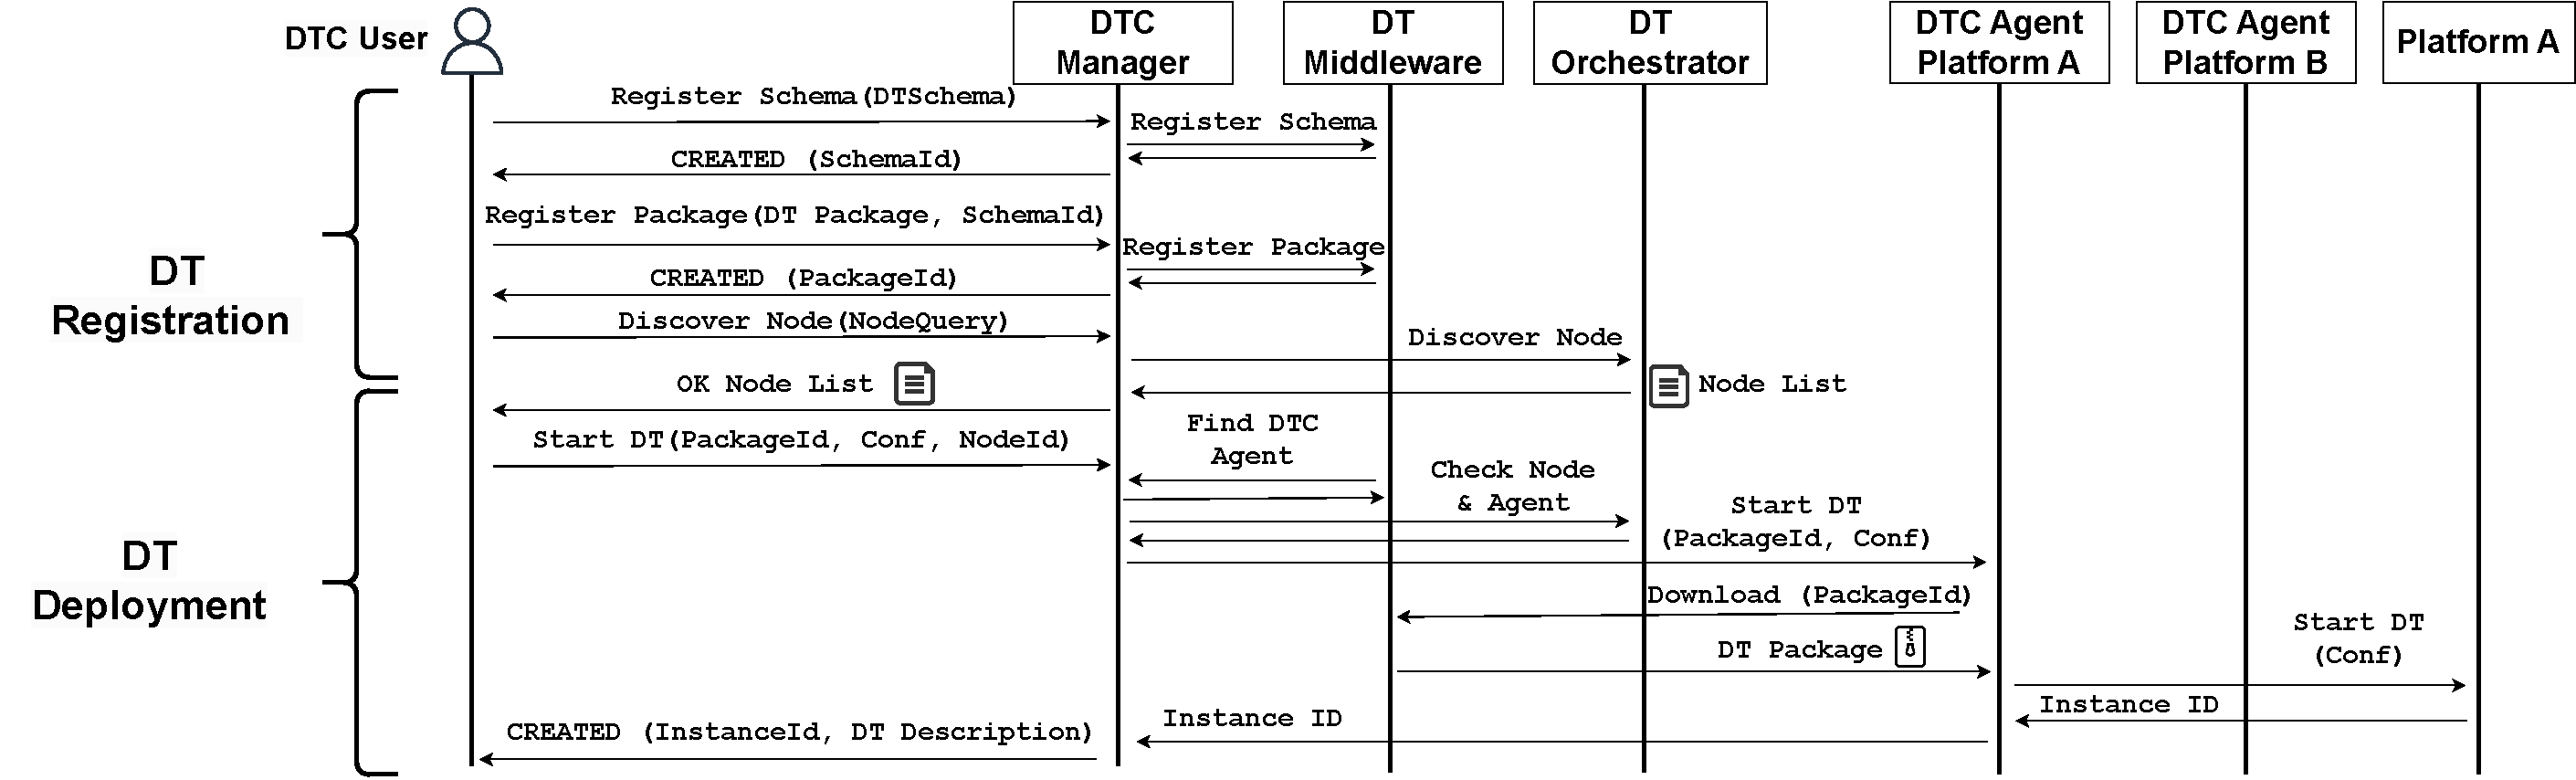
\includegraphics[width=\textwidth]{figures/dtc/sequence_diagram.pdf}
    \caption{The interaction flow example between DTC architectural components to enable DT registration and deployment.}
    \label{fig:dtc-interaction}
\end{figure}

\Cref{fig:dtc-interaction} present an illustrative example depicting a typical interaction scenario among the key components of the DTC architecture.
%
Assuming that the PA has been already registered in the DTC providing the corresponding PAS and PAI descriptions, the figure illustrates the sequence of interactions that occur when a generic user aims to register and deploy a DT for a specific PA.

The initial step to deploy a DT on a target platform involves registering a new DT Schema.
%
All the interactions are facilitated by the DTC Manager, which implements the external-facing API and receives, handles and forwards incoming requests to the appropriate internal component.
%
The request to register a DT Schema is forwarded from the DTC Manager to the DT Middleware. Here, the incoming request is validated, and a new schema is created for the target DT associated with its description, capabilities and fidelity together with the type of physical asset. Subsequently, the DTC manager responds to the user with positive feedback.

The subsequent step entails registering or creating a DT Package linked to the specific schema. The interaction flow follows is similar to the one above, with the DTC Manager receiving the request and the DT Middleware registering the package and associating it with the corresponding SchemaID. 

Moving forward, the registration process for the DTC User involves identifying suitable compute nodes for deploying the target DT. This necessitates a node discovery request initiated by the user, which is forwarded to the DTC Manager.
%
Internally, the DT Orchestrator engages in the discovery process, returning a list of available nodes that match the user's specified criteria, such as the support for package deployment and the support for target hardware requirements (e.g., a GPU for the execution of specific DT's functionalities).
%
The selection of nodes could be automated based on predefined policies. Fort simplicity, in this example, we let the user choose the preferred node from the list of available options.

Upon reviewing the list of available compute nodes matching the target package and schema, the user can proceed by sending a start request to the DTC Manager.
%
This request includes the specific package ID associated with the target schema, along with the starting configuration of the twin which include the identifier of the PAI to which the \ac{DT} will be linked together with the node ID indicating where the DT should be deployed. 
The DTC Manager first verifies compliance of the \ac{DT} package with the platform and the selected PAI, then it checks for the availability of the designated DTC Agent managing the specified node.

Subsequently, it forwards a start request to the target DTC Agent managing the selected platform and node.
%
Here, the DTC Agent checks for the presence of the target DT Package and downloads it if necessary. Once the package is available, the Agent initiates and starts the target DT on the designated platform.
%
Finally, the Agent receives the instance ID of the running DT from the platform and communicates it back to the DTC manager. Subsequently, the DTC manager replies with the instance ID to the user, along with the current description of the running DT instance.

This interaction flow exemplifies the collaborative efforts of the DTC components in facilitating the registration and deployment of DTs, ensuring a seamless experience for users while abstracting the underlying complexities of the infrastructure.
%
By leveraging the descriptions introduced in \Cref{table:dtc_descriptions_requirements}, the DTC effectively manages the lifecycle of DTs, from registration to deployment, while ensuring compatibility with the underlying platforms and compute nodes.

%=======================================================
\section{Proof of Concept Implementation}
%=======================================================


A preliminary analysis, implementation, and experimental evaluation of the core functionalities of the DTC have been conducted using a prototype based on Eclipse Ditto and WLDT as reference platforms.
%
The primary objective of this implementation is to demonstrate the feasibility of the DTC and obtain initial insights by leveraging the microservice capabilities of the White Label Digital Twin (WLDT) library.

The DTC's functional modules (\Cref{fig:dtc-architecture}) are implemented in Python, featuring a \emph{master API} that orchestrates overall behavior and a set of \emph{DTC agents} that manage specific computing nodes and interface with underlying DT platforms such as WLDT and Eclipse Ditto. 
%
These components expose structured RESTful APIs, enabling standardized interaction with the DTC core services. Monitoring and performance tracking across distributed nodes are facilitated through Prometheus, serving as a centralized time-series database, while local agents collect metrics on individual machines.
%
Observability, visualization, and analysis are supported via Grafana dashboards. For the experimental evaluation, the supporting infrastructure—including Virtual Machines (VMs), networking, and container runtimes (Docker and Kubernetes)—was assumed to be preconfigured.


\begin{figure*}[ht!]
    \centering
    \begin{subfigure}{0.49\textwidth}
        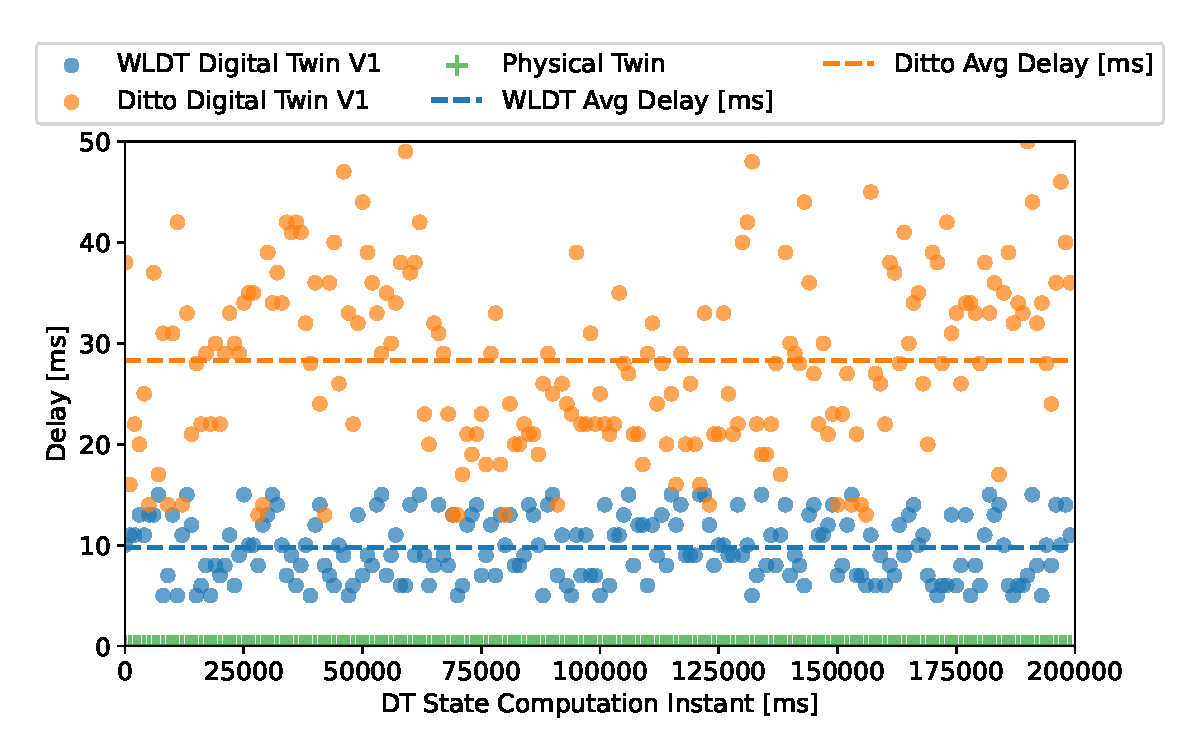
\includegraphics[width=\textwidth]{figures/dtc/wldt_ditto_end_to_end_delay_comparison.pdf}
        \caption{Single DT deployed on both edge and cloud, showing consistent state computation with a small propagation delay between platforms.}
    \end{subfigure}\hfill
    \begin{subfigure}{0.49\textwidth}
        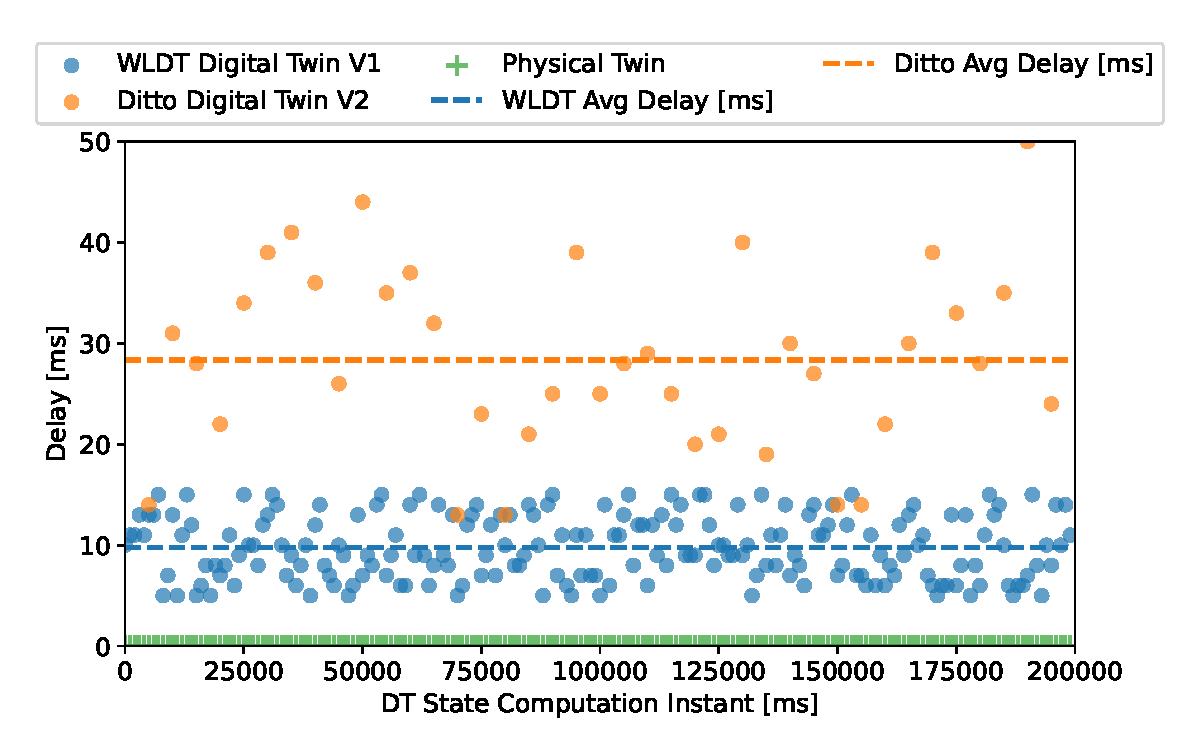
\includegraphics[width=\textwidth]{figures/dtc/wldt_ditto_end_to_end_delay_comparison_2_dts.pdf}
        \caption{Updated cloud DT model with coarser aggregation, illustrating the impact of model versioning and aggregation on state computation relative to the edge DT.}
    \end{subfigure}
    \caption{Comparison of end-to-end DT state computation delays across edge (WLDT) and cloud (Ditto) platforms.}
    \label{fig:exp_single_dt}
\end{figure*}

The \textbf{first experiment} examines the behavior of a single DT deployed across two platforms: WLDT at the edge and Ditto in the cloud. Rather than focusing on communication delays, this experiment aims to demonstrate how the DTC orchestrates state computation and ensures synchronization across multiple DT instances operating on heterogeneous platforms. Two observers, one on the edge and one in the cloud, monitored the propagation and consistency of the DT states.

In the first configuration (Figure \ref{fig:exp_single_dt} left), both DTs run the same model version. The results confirm that the DTC effectively coordinates the two instances, maintaining consistent state computation across edge and cloud, with only minor propagation differences that do not affect overall correctness.

In the second configuration (Figure \ref{fig:exp_single_dt} right), the cloud-based DT is switched to a different, coarser, DT schema (V2) that employs a longer time window for state aggregation (receiving updates from the PA every seconds and computing the state every 5 samples), while the edge DT continues operating with the original high-granularity schema. The DTC seamlessly manages this update, ensuring the cloud DT is correctly deployed and integrated without disrupting the ongoing edge operations. This illustrates the DTC's capability to orchestrate heterogeneous model versions, maintaining consistent, system-wide behavior across distributed DT instances versions and reconcile differences between distributed DT instances.

%%%
\begin{figure}
    \centering
    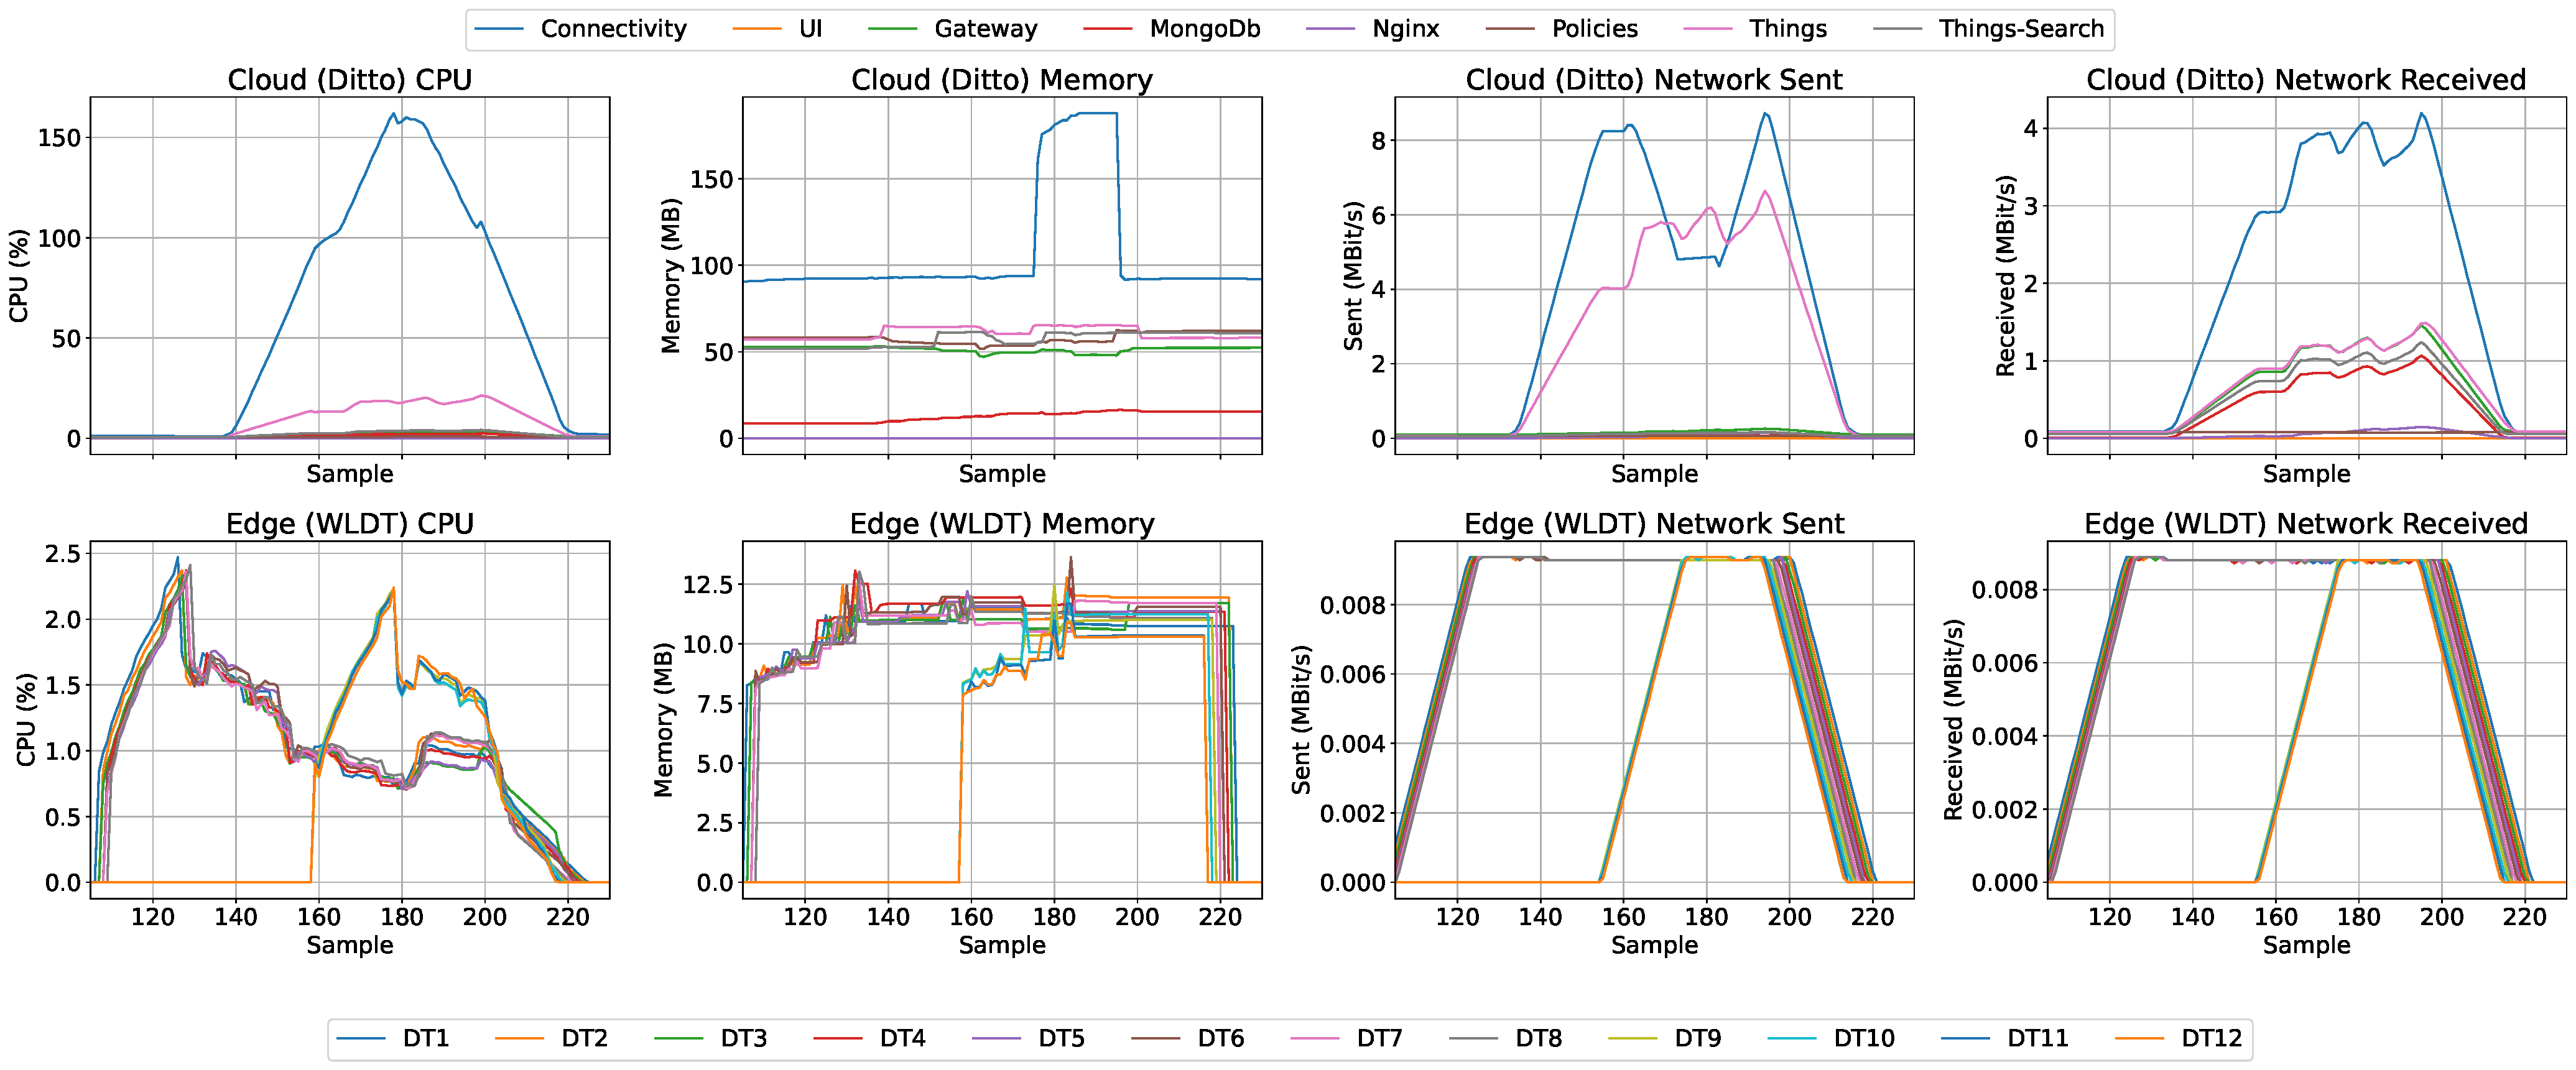
\includegraphics[width=\textwidth]{figures/dtc/edge_cloud_experiment.pdf}
    \caption{Scalability assessment of the DTC prototype in the Microfactory deployment. The figure shows two rows of graphs corresponding to edge (WLDT) and cloud (Ditto) deployments respectively on Edge and Cloud, reporting the evolution of CPU usage, memory consumption, inbound network traffic, and outbound network traffic as the number of active Digital Twin instances increases.}
    \label{fig:dt_resource_usage}
\end{figure}
%%%

The \textbf{second experiment} evaluates the scalability of the DTC prototype in a realistic microfactory deployment (see \Cref{ssec:dte:dt-engineering:scenario} for a description of the microfactory environment).
Performance metrics, including CPU and memory usage as well as network traffic, were monitored during a dual deployment scenario, with Digital Twins instantiated both at the edge (WLDT) and in the cloud (Ditto). The experiment encompasses DTs for individual machines, aggregated DT models for each of the two production lines, and a factory-level DT, totaling twelve distinct DT instances managed by the \ac{DTC}.

Deployment proceeded incrementally along the experimental timeline. Initially, eight DTs were instantiated solely on the edge, followed by the activation of four additional DTs in the cloud, until reaching the full deployment of twelve DTs on both edge and cloud platforms, representing all DT for the microfactory scenario.
%
In this setup, edge DTs exhibit composition behavior compared with the first experiment, while cloud DTs receive their input from edge DTs rather than directly from the physical assets. This configuration allows the DTC to coordinate multiple DT instances across heterogeneous platforms, maintaining synchronization, ensuring consistent communication, and optimizing resource usage as the number of DTs increases.

Measurements captured CPU and memory consumption, as well as inbound and outbound network traffic for each microservice—including core components of Eclipse Ditto and WLDT-based DTs. The results depicted in Figure \ref{fig:dt_resource_usage} illustrate distinct phases of the experiment and highlight the DTC's capability to manage multiple platforms simultaneously. Importantly, the focus is on demonstrating the orchestration and management capacity of the DTC rather than directly comparing the performance of Ditto versus WLDT.

Overall, this proof-of-concept implementation confirms the feasibility and effectiveness of the DTC architecture. The DTC successfully encapsulates the complexity of managing heterogeneous \ac{DT} platforms, providing a unified and coherent view of the industrial system across edge and cloud layers, while maintaining scalability, observability, and system performance under growing operational load.

%=======================================================
\section{Final Remarks}
%=======================================================

This chapter presents the concept of \acl{DTC} as a middleware platform to support the operational management of \ac{DTE} on a compute continuum. 
%
The \ac{DTC} addresses key challenges that emerge when dealing with the deployment and management of systems that involve multiple \acp{DT}, characterized by heterogeneous physical assets, diverse DT platforms, and varying application requirements.

The proposal in this chapter contributes to answering the research question:

\paragraph{\ref{rq:3} How can we support the operational management of DTEs?}

By using structured descriptions that capture the essential characteristics of physical assets, digital twins, and runtime platforms, the DTC enables stakeholders to effectively discover, deploy, and manage DT instances across a distributed infrastructure.
%
The descriptions are designed to be platform and application-agnostic, allowing for seamless integration and interoperability among different DT platforms and use cases.
%
The DTC architecture incorporates key functional components, including a middleware layer and orchestrator, which facilitate the interaction with distributed computing nodes through the abstraction of DTC agents. 
%
This approach supports different stakeholders in their respective roles, offering a coherent holistic view of the DT ecosystem alongside the development-to-deployment lifecycle of its components. 




%%%%%%%%%%%%%%%%%%%%%%%%%%%%%%%%%%%%%%%%%%%%%%%%%%%%%%%%
\chapter{Interoperable \aclp{DTE}}
\label{chap:dte:hwodt}
%%%%%%%%%%%%%%%%%%%%%%%%%%%%%%%%%%%%%%%%%%%%%%%%%%%%%%%%

Answering \ref{rq:2}, this chapter presents a proposal for the engineering of \emph{Heterogeneous} \acp{DTE} (\Cref{chap:dte:dte}).
%
Motivated by the design of the Web and its success in creating interoperability among digital services---more recently, in \ac{IoT} systems through the \ac{WoT} (\Cref{chap:back:Web})---the chapter explores whether and to what extent hypermedia principles and Web standards can be applied to design and implement \acp{DTE}. 
%
The result of this investigation, refines and extend the ideas originally presented in \cite{web-of-dt-ricci-2022}, combining the \ac{WoDT} conceptual model with the design rationale of the Web to build a \emph{\ac{HWoDT}}.

This approach offers a practical implementation strategy for \acp{DTE}, enabling interoperability at both the \ac{DT} and ecosystem levels, and facilitating uniform interaction across \acp{DT} regardless of the underlying technological stack.

The chapter presents the \ac{HWoDT} conceptual integration of hypermedia principles and Web standards in \ac{DTE}, 
and the prototype implementation of a supporting set of tools that demonstrate the feasibility of the approach.


%======================================================
\section{A \acl{HWoDT}}
\label{sec:hwodt-idea}
%======================================================

The main driver of the proposed approach is to support seamless integration of existing \acp{DT}, regardless of their underlying technologies and with minimal overhead.
%
Hence, the core idea is to hide the heterogeneity of \acp{DT} behind a \emph{uniform interface} built with Web protocols and standards, and supported by an explicit semantic layer that allows \acp{DT} to provide a uniform description of both their state and their features and services. 
%
Thus, the name \emph{\acf{HWoDT}}, aims to emphasize the hypermedia-driven nature of the approach, following the \ac{HATEOAS} principle of the \ac{REST} architectural style~\cite{fielding2000architectural}.

Such an interoperability layer enables navigation and seamless interaction with heterogeneous \acp{DT}.
%
To complement it with additional ecosystem-level functionalities, the idea of a \emph{WoDT Platform} is introduced as both a scope boundary defining ecosystem membership and an aggregation layer enabling consumers to query, observe, and exploit services across distributed \acp{DT}.

As illustrated in \Cref{fig:hwodt}, the resulting architecture is composed of \acp{DT}:
\begin{inlinelist}
    \item created using heterogeneous technologies,
    \item implementing the uniform interface through \emph{adapters},
    \item connected by relationships that reflect the physical ones,
    \item and that are aggregated into \acp{DTE} by being registered to one or multiple WoDT Platforms.
\end{inlinelist}    

\begin{figure}[t]
  \centering
  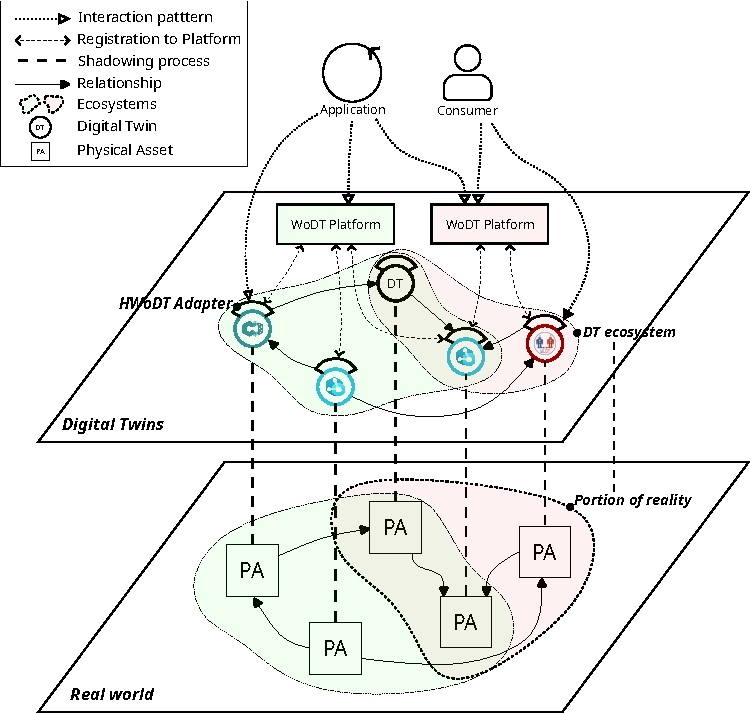
\includegraphics[width=0.7\columnwidth]{figures/hwodt/hwodt.pdf}
  \caption{The Hypermedia WoDT scheme, in the real world PAs (squares) belonging to different organizations and domains are connected by relationships. In the digital world, cross-domain ecosystems of DTs (circles) mirror different portions of reality, supported by the WoDT Platform.}
  \label{fig:hwodt}
\end{figure}

%-----------------------------------------------------------
\subsection{A Uniform Interface for Heterogeneous DTs}
\label{ssec:uniform-interface}
%-----------------------------------------------------------

The first step towards integrating heterogeneous \acp{DT} is to look into how each individual \ac{DT} can expose a uniform interface, compliant with the requirements of the \ac{HWoDT}.
Achieving standard semantic representations of \acp{DT} is an open challenge for the \ac{DT} community.
%
In this work, adopting a pragmatic approach, the benefits of uniform semantic representations in building interoperability are demonstrated through a proposal grounded on the \ac{HATEOAS} principle of the Web architecture:
each \ac{DT} must be able to provide consumers with both \emph{data} and \emph{affordances}---i.e., action possibilities---through hypermedia representations.
This leads to distinguish two logically different representations:
\begin{itemize}
    \item a \emph{\acf{DTD}}, inspired by the \ac{WoT} \acl{TD}, to hold metadata and affordances, enabling consumers to understand the \ac{DT} model, as well as which services the \ac{DT} exposes and how to access them;
    \item a \emph{\acf{DTKG}} representing the live state of the \ac{DT}, semantically encoding domain knowledge and supporting state observation, querying, and discovering relationships between \acp{DT}.
\end{itemize}

Each \ac{DT} is further required to comply with a set of standard \emph{interaction patterns} to allow consumers to uniformly obtain and manipulate such representations for all \acp{DT} in the \ac{HWoDT}.

%.................................
\subsubsection{The \acl{DTD}}
%.................................

The \ac{DTD} serves the primary purpose of providing management metadata about a \ac{DT}, registering it within the ecosystem and describing the exposed interactions\footnote{Documentation on the structure of the \ac{DTD} schema is available on GitHub \url{https://github.com/Web-of-Digital-Twins/dtd-conceptual-model}}.

A primary concern is \emph{identification} of the \ac{DT} and the associated \ac{PA} to unambiguously distinguish them from other elements of the ecosystem.
While \acp{PA} may use domain-specific identifiers (e.g., a serial number), each \ac{DT} in a \ac{HWoDT} is identified with a persistent, globally unique \ac{URI}.
This ensures identification and accessibility of \acp{DT} as Web resources throughout their whole lifecycle.

Furthermore, to support navigation from a \ac{DT} to the ecosystem it is part of, the \ac{DTD} also links to the \ac{URI} of the ecosystem---in the prototype implementation this is a URI served by the \ac{WoDT} platform to identify the \ac{DTE}.

Other relevant metadata in the \ac{DTD} concerns the model used to represent the \ac{PA} at the digital level.
%
The \ac{WoDT} metamodel (\Cref{sec:back:dt:dte})---closely aligned with the  \ac{WoT} \ac{TD}---can describe the \ac{DT} in terms of which properties, relationships, events, and actions are available to \ac{DT} consumers. 

Finally, the \ac{DTD} presents a description of the \ac{API} that consumers can use to interact with the \ac{DT}, using hypermedia controls to describe protocol bindings for the exposed interaction patterns.
%
The \ac{DTD}, is thus aligned with \ac{REST} principles as it presents both data and controls to consumers using self-descripting messages.

Even if the \ac{DTD} may evolve with new properties or interactions when a \ac{DT} gets updated, it remains mostly static as it describes the \ac{DT}'s identity metadata and software interface, not its real-time state.

%.................................
\subsubsection{The \acl{DTKG}}
%.................................

As a \ac{DT} main responsibility is to provide an up-to-date representation of the \ac{PA} state, the \ac{DTKG} complements the \ac{DTD} by representing the live state of the \ac{DT} with a \ac{KG}.

The \ac{DTKG} by means of \ac{RDF} triples, represents:
\begin{itemize}
    \item current property values;
    \item current relationships with other \acp{DT};
    \item context-dependent available actions.
\end{itemize}
Events, generated by the \ac{DT} are excluded from this representation as they are non-persistent information handled via subscriptions.

By using \ac{RDF}, the \ac{DTKG} can represent knowledge about the \ac{DT}'s state with explicit semantics using domain-specific ontologies to support a common interpretation of \ac{DT} data.
Additionally, following the Linked Data principles~\cite{Bizer_Heath_Berners-Lee_2023}, \acp{DT} linking to other \acp{DT} through relationships supports navigating across the ecosystem in a distributed \ac{KG}.

%.............................................
\subsubsection{\acl{DT} Interaction Patterns}
%.............................................

Other than generating the necessary \ac{DTD} and \ac{DTKG} each \ac{DT} in a \ac{HWoDT} ecosystem is required to implement a Web \ac{API} for consumers. This enables direct use by any Web client.

First, the \ac{API} should expose methods to retrieve the two \ac{DT} representations presented above.
%
As the main function of a \ac{DT} is to represent the \ac{PA} state over time, when dereferencing the \ac{URI} which identifies the \ac{DT} with an HTTP GET request the \ac{DT} must return the current \emph{snapshot} of the \ac{DTKG}.

\begin{figure}
    \centering
    \begin{subfigure}[t]{0.45\columnwidth}
        \centering
        \includegraphics[width=\textwidth]{figures/hwodt/dtddtkg.pdf}
        \caption{}
        \label{fig:sequence-dtddtkg}
    \end{subfigure}
    \hfill
    \begin{subfigure}[t]{0.46\columnwidth}
        \centering
        \includegraphics[width=\textwidth]{figures/hwodt/dtdactioncrop.pdf}
        \caption{}
        \label{fig:sequence-action}
    \end{subfigure}
    \caption{Interaction patterns to (a) access the \ac{DTD} and \ac{DTKG} and (b) invoke available actions on a \ac{DT} through the uniform interface and standard Web patterns.}
    \label{fig:sequence-interactions}
\end{figure}



Technically, since a \ac{DT} qualifies as a \emph{non-information resource}\footnote{For a discussion on information vs. non-information resources see \url{https://www.w3.org/TR/cooluris/} and \url{https://lists.w3.org/Archives/Public/www-tag/2005Jun/0039.html}}
the standard Web practice is returning a 303 (See Other) status code with the \textit{Location} HTTP header set to the \ac{URL} of the \ac{DTKG} information resource.
%
The \ac{URL} of the \ac{DTD} is linked in an HTTP Link Header with a custom relation type \texttt{dtd} in the response of the \ac{DTKG} GET request.
%
In this way, consumers can follow links between resources and access both \ac{DT} representations with standard Web interactions as shown in \Cref{fig:sequence-dtddtkg}.

Since the \ac{DTKG} evolves over time to reflect the \ac{PA} state, \acp{DT} are required to support a subscription \ac{API} to observe such changes (e.g., via WebSockets, long-polling, or WebSub~\cite{websub}).
Modeling the \ac{DTKG} as a Web resource also enables basic historicization using protocols like Memento~\cite{rfc7089}, if the \ac{DT} acts as a Memento TimeGate.

Finally, the \ac{API} may expose \ac{DT} actions that can be invoked by external consumers.
The \ac{DTKG} shows which actions are currently valid, while the \ac{DTD} describes how to request their execution to the \ac{DT}.
Consumers rely on both to interact and invalid actions should fail (e.g., with HTTP 403), ensuring consistency with the \ac{DT} model.
%
Figure \ref{fig:sequence-action} illustrates the interaction pattern to invoke an action on a \ac{DT}, by first checking its availability in the \ac{DTKG} and then following the affordance described in the \ac{DTD} to execute it.

%---------------------------------------------
\subsection{Ecosystem Services in the HWoDT}
\label{ssec:ecosystem-services}
%---------------------------------------------

In the proposal for realizing the \ac{HWoDT} ecosystem functionalities described in \Cref{chap:dte:dte} are implemented through a middleware:
%
the \emph{\ac{WoDT} Platform} aggregates data from registered \acp{DT} and exposes an \ac{API} that consumers can use to manage and interact with the ecosystem as a whole.

%........................................
\subsubsection{Managing the \acl{HWoDT}}
%........................................

The \ac{HWoDT} proposal assumes that \acp{DT} are existing, independently running software entities which implement the uniform interface presented in \Cref{ssec:uniform-interface}.
%
Hence, the \ac{DT} creation is handled by developers with their technology of choice, and adding it to an ecosystem is simply a matter of registering it to a \ac{WoDT} Platform. 
%
The platform exposes an \ac{API} that either managers, an external service or a \ac{DT} itself, can use to submit a \ac{DTD} to register a new \ac{DT} to the ecosystem.
The \ac{DTD} is then stored in a registry, which further allows it to be updated or removed if the \ac{DT} leaves the ecosystem.
%
Consumers can also use the registry \ac{API} to discover which \acp{DT} are in the ecosystem and to filter them based on metadata in the \ac{DTD}---e.g., they can discover if multiple \acp{DT} in the ecosystem model the same \ac{PA} filtering on the \ac{PA} identifier.

These simple operations are sufficient to manage the ecosystem. 
%
The \ac{DTD} is used in the registration process as it provides the necessary metadata to assess membership and compliance requirements as well as the \ac{API} description that the platform can use to interact with the \ac{DT} upon registration.
% 
Once registered, the platform uses the \ac{API} description within the \ac{DTD} to access and observe the \ac{DTKG}.  
It can also notify successful registration, enabling the \ac{DT} to record the platform \ac{URI} in its list of ecosystems updating its \ac{DTD} accordingly.

%..........................................
\subsubsection{Exploiting the \acl{HWoDT}}
%..........................................

By observing each individual \ac{DTKG}, the platform can cache the latest update and aggregate them to create a global \ac{DTE} \ac{KG} that can be exploited to implement ecosystem-level services for consumers.
%
The \ac{DTD} and \ac{DTKG} of each \ac{DT} are stored within the \ac{KG}, allowing queries to easily retrieve all available information about a \ac{DT}.
%
Each update of a \ac{DTKG} is processed and merged in the global \ac{KG} so that current representation of the whole ecosystem is always available to consumers.



The \ac{DTE} is a non-information resource and has a \ac{URI} which, when dereferenced, returns the global \ac{DTE} \ac{KG}\footnote{As the ecosystem \ac{KG} can be very large, returning the whole thing can be impractical. Alternatives include returning a partial representation with links to the \acp{DT} caches}.
%
Consumers can also \emph{query} the \ac{DTE} \ac{KG} through the \ac{WoDT} platform SPARQL endpoint.
%
This enables the extraction of selected information from the current state of all \acp{DT} in the ecosystem with a standard query language.

Finally, consumers may want to observe the evolution of the ecosystem \ac{KG}. The platform must then support an \ac{API} to receive subscription requests and send updates to observers.
%
Given the large nature of the \ac{DTE} \ac{KG}, consumers might not be interested in receiving \emph{all} updates. Hence, techniques for \ac{RDF} stream processing~\cite{barbieri2009www} might be more effective to support selective observation.

%======================================================
\section{A Prototype Framework for the HWoDT}
\label{sec:hwodt-impl}
%======================================================

To support the prototyping of heterogeneous \acp{DTE} based on the \ac{HWoDT} proposal, a set of tools is implemented aiming at the integration of existing \ac{DT} technologies.
%
The HWoDT framework is open source and available on GitHub\footnote{\url{https://github.com/Web-of-Digital-Twins}}. 

The software distribution includes a prototype \emph{\ac{WoDT} Platform} implementation and \emph{adapters} to implement the \ac{HWoDT} uniform interface for \acp{DT} developed with \azureTwin{}, \ditto{}, and the \ac{WLDT} framework (\Cref{sec:dte:engineering-dt:wldt-framework}).
%
The technology choice is meant to be representative of the state of the art as they differ in terms of functionalities, namely \azureTwin{} is a cloud platform, Ditto is an open-source platform, and \ac{WLDT} allows developing and deploying \acp{DT} as standalone software processes.
This section presents the overall architecture (\Cref{fig:abstract_arch}) and its implementation.


\begin{figure}
  \centering
  \includegraphics[width=0.8\columnwidth]{figures/hwodt/abstract_arch.pdf}
  \caption{Overall abstract architecture of the \ac{HWoDT} framework, showing the main functional modules. On the bottom existing \acp{DT} which, through the adapter, can implement the \ac{HWoDT} uniform interface and be integrated with a \ac{WoDT} platform.}
  \label{fig:abstract_arch}
\end{figure}



%----------------------------------------------
\subsection{A \ac{WoT}-compatible \acl{DTD}}
%----------------------------------------------

The \ac{DTD} is a central component in the design of the uniform interface of the \ac{HWoDT}.
%
Its design is inspired to the \ac{WoT} \ac{TD}, as an \ac{API} description of the functionalities offered by a \ac{DT}.

Although the \ac{WoT} explicitly reference \acp{DT} in its architectural patterns, the \ac{TD} alone does not support all the metadata that are needed in the proposed \ac{DTD}.
Hence, using \ac{WoT}-compliant mechanisms, \acp{TD} are extended to include the relevant metadata in order to qualify as a functional \ac{DTD} for a prototype implementation of the \ac{HWoDT}.
%
Namely, the \ac{TD} is extended using a custom \emph{\ac{WoDT} vocabulary}\footnote{\url{https://github.com/Web-of-Digital-Twins/wodt-vocabulary}}
which defines concepts to implement the \ac{DTD} and the \ac{DTKG}, as well as HTTP Link Headers relation types used in the interactions of the \ac{HWoDT} (see \Cref{ssec:uniform-interface}).
%
\Cref{lst:dtd-thing-model} shows a generic \ac{TM}~\cite{wot-td} that can be used to implement a valid \ac{DTD}. The \ac{DTD} must include:
\begin{itemize}
    \item the \ac{PA} identifier, 
    \item a link to the \ac{DTKG},
    \item an \texttt{observeallproperties} affordance to subscribe to updates of the \ac{DTKG}.
\end{itemize}

\lstinputlisting[
    label={lst:dtd-thing-model},
    caption={The Thing Model that Thing Descriptions must
    implement to be recognized as a valid \acl{DTD}.},
]{listings/hwodt/dtd.jsonld}


% \begin{figure}
%   \centering
%   \includegraphics[width=\columnwidth]{figures/hwodt/wot-dt-mashups.pdf}
%   \caption{Keeping Digital Twin representations aligned with the \ac{WoT} Thing Description enables the creation of mixed mashups and interoperability with existing \ac{WoT} consumers.}
%   \label{fig:wot-dt-mashups}
% \end{figure}

The alignment with the \ac{WoT} is strategic for the \ac{DT} community as reusing the existing standard ensures compatibility and favors the development of application mashups.
%
The \ac{DTD} can be served by the \ac{DI} of a \ac{DT} to be discovered and consumed by existing \ac{WoT} clients (see \Cref{sec:dte:engineering-dt:physical-digital-adapters}).
%
Clients that have the capability to interpret the \ac{WoDT} vocabulary can then exploit the additional metadata to interact with the \ac{DT} as part of a \ac{HWoDT} ecosystem as shown in \Cref{fig:wot-dt-mashups}.

%-----------------------------
\subsection{HWoDT Adapters}
\label{ssec:adapters}
%------------------------------

\acp{DT} in a \ac{HWoDT} ecosystem must all adhere to the uniform interface, regardless of the technology used to implement them.
%
Adapting existing \ac{DT} technologies to the \ac{HWoDT} interface requires aligning data and interaction patterns.
%
To show that this alignment is achievable with configurable reusable components a set of \emph{adapters} is developed to integrate some mainstream technologies within a \ac{HWoDT} ecosystem.
%
All adapters support HTTP interactions and WebSocket-based \ac{DTKG} observation.
%
The abstract architecture followed by all adapters is shown in \Cref{fig:abstract_arch}, bottom.

%..............................................
\subsubsection{\azureTwin{} Adapter}
%..............................................

\azureTwin{} is Microsoft's domain-independent \ac{PaaS} \ac{DT} solution, supporting the management of multiple \acp{DT} connected within a \emph{twin graph}.

Creating \acp{DT} in \azureTwin{} requires defining their model using the \emph{\acf{DTDL}}, a custom JSON-LD format to specify properties, relationships, commands (actions) and telemetry (events) that describe a \emph{type} of \ac{DT}.
%
\ac{DTDL} models can then be used to create \ac{DT} instances.
%
Although the model closely aligns with the \ac{WoDT} model, the support of events and actions is partial\footnote{As of June 2025, commands can be defined but not invoked automatically, while telemetries are not used within \azureTwin{} \url{https://learn.microsoft.com/en-us/azure/digital-twins/concepts-models}} and relationships are limited to linking \acp{DT} within the same \azureTwin{} instance, which hence defines a closed homogeneous ecosystem.

The \azureTwin{} adapter is implemented as a middleware, connecting to an \azureTwin{} instance and mapping \acp{DT} to the \ac{HWoDT} uniform interface.
%
The adapter can be configured to select which \acp{DT} needs to be mirrored and specify the mapping from \ac{DTD} properties and relationships to produce the \ac{DTKG}. 
%
\Cref{fig:azure-adapter-c&c} shows the adapter architecture and the necessary components to connect to an \azureTwin{} instance.
%
The following Azure service pipeline must be set up to link the \azureTwin{} instance to the adapter:
\begin{itemize}
    \item \textit{Azure Event Grid} to capture and forward \azureTwin{} events;
    \item \textit{Azure Function} (\acl{FaaS}) to fetch the current \ac{DT} state and send it to the adapter via SignalR on every new event;
    \item \textit{Azure SignalR} to deliver \acp{DT} state updates to the adapter.
\end{itemize}

The adapter can be deployed either within the Azure cloud or is designed to automatically retrieve the \ac{DTDL} models, stored on \azureTwin{}, and convert them in valid \acp{DTD} for each \ac{DT} instance.
The adapter waits for SignalR events to receive \ac{DT} state updates generated by the Azure Function and convert them into \acp{DTKG} updates.

\begin{figure}
    \centering
    \includegraphics[width=\textwidth]{figures/hwodt/adtadapter-c&c.pdf}
    \caption{The \azureTwin{} adapter, implemented as a standalone component that maps specific instances of \acp{DT} hosted on an \azureTwin{} instance.}
    \label{fig:azure-adapter-c&c}
\end{figure}

%..............................................
\subsubsection{Eclipse Ditto Adapter}
%..............................................

\emph{Eclipse Ditto}, is an open-source \ac{DT} platform from the Eclipse Foundation. 
It abstracts each \ac{PA} as a \emph{Ditto Thing} and offers a Web-based layer for interacting with \ac{IoT} devices through their \acp{DT}.
%
A Ditto instance can manage multiple \acp{DT}, using a metamodel with:
\begin{itemize}
    \item \emph{Attributes} for static metadata,
    \item \emph{Features} which can group data (properties) and functionalities (messages).
\end{itemize}
Although lacking native support for relationships, actions, and events, these can be modeled using attributes (for links), consumer-to-\ac{DT} messages (for actions), and \ac{DT}-to-consumer messages (for events). Models can be defined via a custom JSON format or a (set of) \ac{WoT} \ac{TM}.

Eclipse Ditto is implemented with a microservice architecture. 
Despite Ditto being open-source and allowing the development of custom extensions, the prototype adapter is implemented as a custom external middleware that can be deployed to map one Ditto Thing to the \ac{HWoDT} uniform interface.
%
The middleware leverages Eclipse Ditto's native WebSocket interface to retrieve data and performs two key transformations: converting the \ac{WoT} \ac{TD} exposed by Ditto into a \ac{DTD}, and serializing \ac{DT} data into a \ac{DTKG}.
This process relies on a configurable mapping between Ditto features and their corresponding \ac{RDF} representations.

\begin{figure}[ht]
  \centering
  \includegraphics[width=0.8\columnwidth]{figures/hwodt/ditto-adapter-c&c.pdf}
  \caption{The Eclipse Ditto adapter, implemented as a standalone component that maps a specific instance of a \ac{DT} hosted on the Ditto platform.}
  \label{fig:ditto-adapter-c&c}
\end{figure}

%..............................................
\subsubsection{\acl{WLDT} Adapter}
%..............................................

The \emph{\acf{WLDT} framework} (\Cref{sec:dte:engineering-dt:wldt-framework}) enables the development of \acp{DT} as standalone software components deployable across cloud or edge environments.
%
Specifically, the adapter is implemented as a \ac{DiA}, used in the \ac{WLDT} architecture to represent digital interfaces through which the \ac{DT} can expose data for consumers.
%
The framework internal metamodel is already aligned with the \ac{HWoDT}, so no additional effort is required to map concepts.
The adapter is provided as a reusable Java library, which \ac{WLDT} developers can easily import into their projects and then configure the mapping towards the \ac{HWoDT} uniform interface leveraging the implementation of the necessary \ac{API} to manage the \ac{DTD} and \ac{DTKG}.

\begin{figure}[ht]
  \centering
  \includegraphics[width=\textwidth]{figures/hwodt/wldt-adapter-c&c.pdf}
  \caption{The architectural diagram of the \ac{WLDT} adapter, illustrating its integration with the other components of the framework.}
  \label{fig:wldt-adapter-c&c}
\end{figure}


%..............................................
\subsubsection{Implementing Custom Adapters}
%..............................................
The description of the adapters implemented in the prototype \ac{HWoDT} framework should be useful for any \ac{DT} developer wishing to implement a custom adapter for their own \ac{DT} or \ac{DT} technology. 
%
The idea of the \ac{HWoDT} is grounded on the fact that implementing such custom adapters is relatively straightforward and that the little effort spent in developing (or even less in configuring) them can bring benefits in the integration with the \ac{HWoDT} ecosystem.

To summarize, the steps to develop a custom adapter are: 
\begin{enumerate}
    \item understand how to map the concept of the original \ac{DT} model into the \ac{WoDT} metamodel;
    \item understand how to represent the state of the \ac{DT} with an evolving semantic representation for the \ac{DTKG};
    \item implement a module that can reactively produce the \ac{DTKG} whenever the \ac{DT} state is updated;
    \item implement a module that can serve the \ac{DTD} over HTTP, alongside the mandatory \ac{API} for \ac{DTKG} observation.
\end{enumerate}

%-----------------------------------
\subsection{The WoDT Platform}
%-----------------------------------

A prototype of a \ac{WoDT} Platform is implemented in Kotlin.
The platform implements the modules of the abstract architecture shown in \Cref{fig:abstract_arch}, top as shown in \Cref{fig:platform-c&c}.
%
Namely, the platform offers multiple interfaces for consumers: an HTTP \ac{API} for \ac{DTE} management (Ecosystem Management Interface) and one for \ac{KG} access with a SPARQL endpoint for read-only queries, as well as a WebSocket endpoint to observe ecosystem updates (\ac{WoDT} Platform Interface).

The platform can process the \ac{WoT}-based \ac{DTD} described above to register \acp{DT}.
When a registration requested is submitted, the platform:
\begin{enumerate}[label=\textbf{Step \arabic*}, leftmargin=5.3em]
    \item locates the \ac{DTKG} observation form (\texttt{observeallproperties}) and starts observing the \ac{DT} for updates;\label{step:observe-dtkg}
    \item notifies the \ac{DT} of successful registration to let it update its \ac{DTD} with the platform URI;\label{step:notification}
    \item maps the \ac{DT} \ac{URI} to a local cache URL;
    \item observes \ac{DTKG} updates and merges them into the \ac{DTE} \ac{KG} stored in memory with Apache Jena.
\end{enumerate}

%
The current prototype supports the observation of \ac{DTKG} through WebSockets for \ref{step:observe-dtkg} and implements \ref{step:notification} sending a request to a hardcoded \texttt{/platform} HTTP endpoint on the \ac{DT}.

Consumers can interact with the \acp{DTE} through the \ac{WoDT} platform
either through (possibly repeated) SPARQL queries to retrieve the information they need or by observing the whole \ac{KG} through WebSockets.
%
In the prototype, all observers receive the whole \ac{KG} whenever there is an update so that consumers don't need to have specific update handling logic.
%

\begin{figure}
  \centering
  \includegraphics[width=\columnwidth]{figures/hwodt/platform-c&c.pdf}
  \caption{\ac{WoDT} Platform modules and interfaces, represented using components and connectors.}
  \label{fig:platform-c&c}
\end{figure}


%=======================================
\section{Comparison with Related Works}
%=======================================

This section compares the \ac{HWoDT} proposal with related approaches that target the integration of \acp{DT} in ecosystems. 
%
The aim of this comparison is to highlight the similarities and differences with existing solutions, discussing advantages and limitations of existing approaches with respect to the \ac{HWoDT}.

The \ac{HWoDT} proposal is not meant to compete with existing standards or framework, but rather to either complement them or provide an alternative approach to \ac{DT} interoperability.
%
The main principle of the \ac{HWoDT} is to promote interoperability through the adoption of \ac{REST} principles and Semantic Web technologies, given their proven effectiveness in enabling integration across heterogeneous systems on the Web.


%----------------------------------------------------
\subsection{HWoDT vs. Industrial Standards}
%----------------------------------------------------

The \ac{HWoDT} tackles the relevant issue of enabling \ac{DT} interoperability targeting the creation of \emph{heterogeneous \acp{DTE}}.
%
This is an open challenge in the \ac{DT} research community (see \Cref{sec:back:dt:interoperability}), and several interoperability frameworks are being proposed to streamline the integration of \acp{DT}~\cite{Barnard_2024}.
%
Among the most relevant standards some of the most relevants are \ac{OPC-UA}, \ac{AAS}, \ac{AML} and the \ac{W3C} \ac{WoT}. \Cref{tab:interop_comparison} summarizes a comparison of these standards across selected aspects.

Given the different nature of these standards, they can be viewed as complementary rather than competing against each other.
%
There have been integration efforts in order to leverage their different strengths. For instance, \ac{OPC-UA} has been integrated with web technologies~\cite{DBLP:journals/csi/CavalieriSS19} to support direct integration with web clients, operations in \ac{AAS}~\cite{platform_i40_aas_part1_v2} and affordances in \ac{WoT}\footnote{\url{https://profiles.opcfoundation.org/workinggroup/97}} can have an \ac{OPC-UA} protocol bindings, and \ac{AML} specifications can be linked to \ac{AAS} to have a coherent view of the involved assets~\cite{DBLP:conf/etfa/DrathRH19,DBLP:conf/indin/WengerZ018}.
%
In this view, the Semantic Web technologies adopted in the \ac{HWoDT} approach can be integrated on top of existing standards and complement their features.

\begin{table*}
    \centering
    \small
    \setlength{\tabcolsep}{3pt} % reduce inter-column spacing
    \renewcommand{\arraystretch}{1.3} % slightly tighter rows
   \begin{tabular}{>{\raggedright\arraybackslash}p{2cm}|>{\raggedright\arraybackslash}p{2.2cm}|>{\raggedright\arraybackslash}p{2.2cm}|>{\raggedright\arraybackslash}p{2.2cm}|>{\raggedright\arraybackslash}p{2.2cm}|>{\raggedright\arraybackslash}p{2.2cm}}
    \toprule
    \midrule
    \textbf{} & \textbf{AAS} & \textbf{OPC-UA} & \textbf{AML} & \textbf{WoT} & \textbf{Semantic Web} \\
    \hline
    \hline
    \textbf{Scope} &
    Asset digital representation &
    Device data / \ac{M2M} &
    Tool interoperability &
    Web-scale access &
    Cross-domain knowledge \\
    \hline
    \textbf{Data model} &
    Submodels + semantic IDs &
    Hierarchical node graph (address space) &
    Hierarchies (CAEX, CAD, PLCopen) &
    Thing Description (JSON-LD) &
    Triple Graphs (RDF / OWL) \\
    \hline
    \textbf{Semantics} &
    Structured submodels, semantic references &
    (Sub)Types and Relationships &
    Role-based, structural  &
    JSON-LD semantics, ontology-aligned &
    General-purpose ontologies \\
    \hline
    \textbf{Querying and Data access} &
    REST API &
    Browse address space &
    File access &
    SPARQL (if RDF-mapped) &
    SPARQL / Web browsing \\
    \hline
    \bottomrule
    \end{tabular}
    \caption{Comparison of interoperability frameworks across selected aspects.}
    \label{tab:interop_comparison}
\end{table*}


The Semantic Web excels at general-purpose knowledge representation, and integration of such heterogeneous knowledge under a uniform interface (\Cref{sec:back:web:semantic-web-technologies}).
%
Additionally, it enables reasoning through ontological inference and expressive queries across concepts, supporting use cases that have limited support when using the aforementioned standards alone (see \cref{tab:interop_comparison}, Querying and Data access).
%
It is then not surprising that alignment between Semantic Web technologies and industrial standards are being investigated, highlighting similarities between e.g., \ac{OPC-UA}~\cite{DBLP:conf/etfa/MajumderWD19,DBLP:conf/etfa/PerzyloP0K19} and \ac{AAS}~\cite{DBLP:conf/icphys/BedenCB21, platform_i40_aas_part1_v2} data models, to benefit from these features.

The \ac{HWoDT} proposal, follows this trend, suggesting that the hypermedia layer can serve as an integration on top of existing \acp{DT}, which may already have an implementation based on industrial standards.
%
Additionally, since the described interoperability standards emerged from the Industry 4.0 movement, they generally target only industrial domains. This poses a significant gap when needing to map concepts and represent entities from different domains.
%
The \ac{HWoDT} approach, addresses this gap through the use of Web ontologies which have been developed for a high variety of application domains and can be seamlessly integrated within the same \ac{KG}.

Finally, providing a synchronized representation is a key feature of \acp{DT}.
The \ac{HWoDT} approach, designed with a \ac{DT}-centric perspective, requires each \ac{DT} to produce and update such representation of its current state through the \ac{DTKG}. This supports consumers in both querying an up-to-date view of the whole ecosystem and observing changes on the \ac{DT} state.
%
Similar behavior can be implemented by \ac{AAS} servers (e.g. Eclipse BaSyx\footnote{\url{https://eclipse.dev/basyx/}}) that automatically retrieve data from \ac{OPC-UA} endpoints, but is limited by the expressiveness of queries on the \ac{AAS} model typically relying on Web APIs with no hypermedia support.

Overall, the comparison shows that the \ac{HWoDT} approach is compatible and complementary to existing \ac{DT} interoperability efforts and follows existing research directions aimed at bridging the Semantic Web on top of industrial standards.
The approach can be used as an additional layer integrating \acp{DT} implemented with (or without) other standards to support:
\begin{itemize}
    \item integration with \acp{DT} outside the industrial domain,
    \item advanced query with reasoning on semantic structures,
    \item simple Web-based navigation and direct access to the up-to-date representation of the mirrored asset,
    and 
    \item subscription to changes in the \ac{DT} state.
\end{itemize}

%-------------------------------------
\subsection{HWoDT vs. WoT mashups}
%-------------------------------------

Leveraging the \ac{HWoDT}, developers can focus only on application logic, abstracting away the complexity of heterogeneous \ac{DT} integration.  
This yields two important advantages that are shared with the \ac{WoT} approach:  
\begin{inlinelist}
    \item the application layer is more stable as it remains unaffected by the introduction of new \acp{DT};
    and  
    \item the \ac{DT} layer can evolve or replace underlying implementations without affecting upper layers as long as the exposed interface is not changed.
\end{inlinelist}

Still, a fundamental difference between the \ac{HWoDT} and the (semantic) \ac{WoT} is the ability to seamlessly browse a \ac{KG} of the \ac{DTE} that captures explicitly the \acp{DT}' observable state. 
%
In a W3C \ac{WoT} application, even if \acp{TD} were to be semantically annotated and stored in a \ac{KG}, selecting \emph{things} based on their state properties would require sending the necessary requests to retrieve the current value of each property of each thing.
%
This is because the W3C \ac{WoT} is not tailored to the requirements of \acp{DT}, which, instead, are by definition capable of shadowing---and thus to always show the current state of the asset they represent.
%
Furthermore, the W3C \ac{WoT} does not specify how to handle dynamic relationships between things, limiting the possibility of expressing powerful queries on the state of interrelated assets.
%
The \ac{HWoDT} proposal, leverages this \ac{DT}-specific feature through the \ac{DTKG} component, simplifying the interaction. 
%
Similarly, even when dealing with a set of heterogeneous \acp{DT}, without the unifying abstraction of the \ac{HWoDT}, consumers would need to retrieve the \ac{DT} state representation from each individual \ac{DT}, interpret them and merge the data to resolve the query (\Cref{fig:comparison-custom-vs-hwodt}).

\begin{figure}
  \centering
  \includegraphics[width=\columnwidth]{figures/hwodt/comparison_custom_hwodt.pdf}
  \caption{Comparison of the steps required to perform a ``query'' across heteregenous \acp{DT} versus with the \ac{HWoDT} approach, which abstracts heterogeneity through a uniform interface.}
  \label{fig:comparison-custom-vs-hwodt}
\end{figure}

%-------------------------------------------------------
\subsection{HWoDT vs. Closed DT Platforms}
%-------------------------------------------------------

The \ac{HWoDT} approach, offers a solution to implement open \acp{DTE} on top of heterogeneous \ac{DT} technologies.
%
This contrasts with the vision of other \ac{DT} platforms which, instead, support homogeneous \acp{DTE} and offer support for the definition of multiple \acp{DT} within the same instance, but constraining all of them to adhere to specific technological choices.

The most recognized technology for building \acp{DTE} is the off-the-shelf solution offered by \acl{ADT}.
The graph-based rationale within the platform has been an inspiration for the \ac{HWoDT}, as a way to connect multiple \acp{DT} and obtain a cohesive view of the physical reality.

Still, \acl{ADT} is a Platform-as-a-Service solution, only available through the Azure cloud, strongly limiting its application in different scenarios where the \acp{DTE} might be constructed on a private infrastructure.
%
The technological stack is completely custom, creating a vendor lock-in on the developed \acp{DT} models.
% 
Azure requires \acp{DT} to be defined using its own custom \ac{DTDL}, supports only custom ontologies (or requires converting existing ones form \ac{OWL} to \ac{DTDL}) and supports queries on the \emph{twin graph} only through a custom SQL-like query language.
%
Furthermore, in closed approaches, it would not be possible to create relationships with entities that are outside of the supporting platform. For instance, the relationship model of \azureTwin{} requires to define possible relationships between \ac{DTDL} models.
%
The \ac{HWoDT} addresses this limitation by enabling the definition of cross-platform \ac{DT} relationships using Linked Data principles.   
This enhances the expressiveness of \acp{DTE} and allows developers to model ecosystems that more accurately reflect domain knowledge.

Through the \ac{HWoDT} we reclaim the vision of open \acp{DTE} that can be enabled by a stack of open standards and technologies. 
%
This offers an alternative to closed platforms, allowing the development of \acp{DTE} in a variety of different settings tailored to the specific use case needs.

Although open-source \ac{DT} platforms like the aforementioned Eclipse Ditto exist, they have not being designed with an ecosystem perspective in mind. 
Differently from the \ac{HWoDT}, platforms like Ditto merely support having multiple instances of \acp{DT} hosted on the same platform and exposing similar \ac{API}. 
%
This constraints the \ac{DT} implementation to adhere to Ditto models, protocols and \ac{API}, does not offer native support for tracking meaningful dynamic relationships between assets and has very limited query capabilities\footnote{Ditto supports queries through a search \ac{API} based on the Resource Query Language \url{https://eclipse.dev/ditto/basic-search.html}}


%-------------------------------------------------------
\subsection{HWoDT vs. Other Web-based DTs}
%-------------------------------------------------------


The \ac{HWoDT} is not the first attempt to leverage Web features in \acp{DT} implementations. Service-oriented and micro-service architectures are among the most prominent architectural patterns when it comes to implementing \acp{DT} according to a recent survey~\cite{ferko2022architecting}, making a strong parallel with Web services.

In \cite{Liu_Jiang_Jiang_2020} the authors propose a Web-based approach for the development of \acp{DT} of a production system.
They leverage a multi-layer architecture with the uppermost layer exposing \ac{REST} \acp{API} and ontologies to describe the components of a \ac{CPS} using the abstraction of production nodes.
%
Although the approach shares some similarities with the \ac{HWoDT} proposal in enabling a uniform interface to organize modules of a \ac{CPS}, it is heavily restricted to the manufacturing domain and, crucially, it relies on all the production nodes to use the same technological stack and does not include heterogeneous \acp{DT}.

In \cite{Autiosalo_Siegel_Tammi_2021} the authors propose an approach for a \emph{Digital Twin Web} and an open-source implementation of a Web server to host \ac{DT} description documents called Twinbase through Git-based workflows.
%
The approach shares the main motivations that are behind the \ac{HWoDT} proposal, leveraging Web standards to promote interoperability and connect \acp{DT} in a network that any consumer can access with a Web browser. The main goal is to provide a meta-level registry of \acp{DT} so that consumers can discover them and also shares the idea of having relationships between \ac{DT} instances.
%
Despite these similarities, the approach differs for several reasons. First, the proposed description is not using any semantics, enforcing a very basic model for representing the \acp{DT} using Yaml files. Second, the represented \acp{DT} are mostly static, and do not share their state in a uniform way but only link to other resources or \acp{API} to interact with the \ac{DT} state under a set of generic \emph{features} the \ac{DT} can expose. Third, the proposed architecture based on Git workflows is limiting to a very specific subset of applications that can deal with that kind of interface to publish updates.

Finally, other approaches exploit the \ac{WoT} in the context of \acp{DT}. In this work, the \ac{WoT} \acp{TD} is semantically extended to implement a preliminary \ac{DTD}. 
%
A similar extension is presented in \cite{González-Gerpe_Cimmino_Bernardos_Poveda-Villalón_García-Castro} which proposes to use the \ac{TD} ontology in the construction domain, extending it to capture the five-dimensional model of \acp{DT}~\cite{qi2021enablingtechdt}.
%
The \ac{WoT} is also the foundation of WoTwins~\cite{SciulloWoTwins2022} a framework to generate automatically \acp{DT} starting from existing \ac{WoT} things, modeling their behavior and enabling prediction features. 
%
These works highlight the relevance of the \ac{WoT} as a standard for the future of \ac{DT} applications, despite its limitations in capturing fully the nature of a \ac{DT} in its entirety which may require extensions and development of custom ontologies aligned with the \ac{WoT} model.

%==========================================
\section{Prototype Performance Evaluation}
%==========================================

A performance evaluation of the prototype is carried out to quantify the performance implications introduced by the additional layer introduced by the \ac{HWoDT} to implement \acp{DTE}.
%
\Cref{fig:latency-hwodt} schematically shows the communication between components in a \ac{HWoDT}-based system. \circled{A} is the latency between \ac{PA} and \ac{DT}, \circled{B} is the latency between the \ac{DT} and the \ac{HWoDT} adapter, \circled{C} is the latency between the adapter and the platform, while \circled{D} is the latency between the platform and the client. In a scenario where the DT is used without the platform \circled{E} would be the latency between the DT and the client. This shows that the additional potential latency loss in a \ac{HWoDT} system is given by \circled{B}+\circled{C}.

\begin{figure}
  \centering
  \includegraphics[width=0.8\columnwidth]{figures/hwodt/HWoDT-latency.pdf}
  \caption{Latency in an HWoDT-based system.}
  \label{fig:latency-hwodt}
\end{figure}

Accordingly, the following evaluation assesses the performance of the \ac{HWoDT} platform prototype, thereby characterizing the overhead incurred when integrated atop existing interoperability standards.
Even though performance optimization was not a primary focus in the development of the \ac{HWoDT} platform prototype, it can still be useful to make some considerations on the performance of the \ac{HWoDT} approach.
%
To do so an experimental setup is used to measure the latency \circled{B}+\circled{C}+\circled{D} when interacting with the platform and compare it with \circled{E}.

%-----------------------------------
\subsection{Experimental Setup}
%-----------------------------------

The experiment is designed to stress the performance of the platform in a resource-intensive scenario, and measure the delay perceived by consumers wishing to interact with \acp{DT} and the ecosystem as a whole.
%
A synthetic workload is used because---differently from a real-world \ac{IoT} dataset which may include data spikes over time---the scenario allows us to have a fully controllable environment to scale the traffic and evaluate the response of the platform under different loads.

A \ac{DTE} of a network of temperature sensors is implemented, with \acp{DT} reporting an update every second using \acp{DT} implemented with the \ac{WLDT} framework, running within the same process.
%
Each \ac{DT} generates a random temperature value between 0 and 100 every second, with a random initial offset of up to one second to avoid perfect synchronization of the \acp{DT}' data streams. The \ac{DT} state includes a timestamp marking when the state was computed by the \acp{DT}.
%
The different interaction patterns of the \ac{DTE} are tested:
\begin{itemize}
    \item with clients \emph{observing} all the \acp{DT} receiving all the \acp{DT} state notifications;
    \item with clients periodically \emph{querying} the \ac{DTE} to retrieve all sensors that have a reported temperature greater than 50. 
\end{itemize}
%
The key metrics collected are the \emph{freshness} of the information, which is computed as the difference between the time a state notification is received and the timestamp of the message (or the greatest timestamp when observing the \ac{DTE} \ac{KG}).
%
Additionally, the time taken to perform a query on the ecosystem retrieving the state of all \acp{DT} matching a condition is measured.

The experiments have been carried out running the \acp{DT} the \ac{WoDT} platform and the client applications on the same machine equipped with a 13th Gen Intel(R) Core(TM) i7-13700H CPU and 32 GB of RAM, using the OpenJDK 21.0.7 runtime.
%
Data is collected by analyzing logs of the client applications.

All \acp{DT} have been implemented with the \ac{WLDT} framework. 
The framework supports defining \ac{DT} implementations and uses a plugin-based architecture to expose different interfaces. 
This has been useful to implement different interaction patterns for the same \ac{DT}.

Measurements are repeated with 50, 100 and 200 \acp{DT}, and performing operations with 1, 50, 100 clients each observing all \acp{DT} and querying the entire \ac{DTE}.


%-----------------------------------
\subsection{Results}
%-----------------------------------

This section briefly reports results of the performance evaluation focusing on the different interaction patterns of the \ac{WoDT} platform prototype and comparing them with baseline direct interactions with individual \acp{DT}.
%
The results are summarized in \Cref{fig:sequence-interactions}, showing two bar plots reporting the average values of the two metrics collected in the experiments.
%
Results confirm that the overhead introduced by the \ac{HWoDT} platform is not negligible, but still acceptable for many \ac{DT} applications, especially when considering the benefits of having a uniform interface to interact with heterogeneous \acp{DT}, especially when considering the ability to query the whole \ac{DTE} \ac{KG}.

\begin{figure}
    \centering
    \begin{subfigure}[t]{0.49\textwidth}
        \centering
        \includegraphics[width=\textwidth]{figures/hwodt/mean_latency_barplot.pdf}
        \label{fig:observation-delay}
    \end{subfigure}
    \hfill
    \begin{subfigure}[t]{0.49\textwidth}
        \centering
        \includegraphics[width=\textwidth]{figures/hwodt/mean_request_time_barplot.pdf}
        \label{fig:query-time}
    \end{subfigure}
    \caption{Performance indicators with different loads of \acp{DT} and clients working on the ecosystem: (a) average time difference when observing \acp{DT} either directly or through the \ac{WoDT} platform, and (b) average time per operation when querying the DT ecosystem either through the \ac{WoDT} SPARQL endpoint or directly retrieving the state from each \ac{DT} API.}
    \label{fig:sequence-interactions}
\end{figure}

%...................................
\subsubsection{\aclp{DT} Observation}
%...................................

The \ac{HWoDT} adapter sends updates of the \ac{DTKG} on a WebSocket connection to the platform. Clients are set up to connect to the platform and observe each \ac{DT} through a WebSocket connection.
This aims to measure the delay introduced by the communication between the adapter and the platform, before getting to a final consumer. 
%
As the platform also supports observing the full \ac{DTE} \ac{KG}, a client also observes directly the \ac{KG} updates over a WebSocket connection (\circled{B}+\circled{C}+\circled{D}).
%
This is compared against direct observation of the \ac{DT}, which is implemented by sending each state update to an MQTT broker. Clients connect to all topics \texttt{dt/+/state} to observe all \acp{DT} (\circled{E}).

Whenever a message is received, the \emph{freshness} metric is computed as the difference between the timestamp of the message and the time the message is received using the system clock (which is synchronized as all processes run on the same machine). 
%
For the \ac{DTE} \ac{KG} as a new state update is generated for each change of each \ac{DT}, the greater timestamp among all \acp{DT} is taken to compute the freshness.

\Cref{fig:observation-delay} shows the average time difference with the different observation techniques. 
As expected, directly observing individual \acp{DT} is more efficient, as there is virtually no overhead. Users of the \ac{WoDT} platform should prefer this whenever possible, following the affordances of \acp{DT} in the \ac{DTD}.
%
In all scenarios, the delay grows with the number of \acp{DT}. This is especially evident when considering the observation of the whole \ac{DTE} \ac{KG}, which is the least efficient. Analyzing the performance of the prototype it was possible to deduce that this is caused by the serialization of the whole \ac{KG} to stream it at every update, which is computationally intensive. 
%
This is also the reason why the figure avoids reporting the observation of the ecosystem \ac{KG} with more than 1 client, as the results are significantly worse than the other options, even with just 1 client.
Performances are expected to be less drastically impacted when using smarter \ac{KG} update notification strategies---such as sending incremental changes (e.g., as in \cite{roffia2018fi})---at the cost of requiring more complex clients, capable of applying the changes to reconstruct the full state.

%...................................
\subsubsection{Repeated Querying}
%...................................

Clients can query the \ac{DTE} through the SPARQL endpoint of the \ac{WoDT} platform.
%
This is compared with performing an interrogation directly on all \acp{DT} to retrieve the current state and then filtering it on the client side which is implemented by having all \acp{DT} expose a simple HTTP endpoint \texttt{GET /state} to retrieve the current state of the \ac{DT} (similarly to what is shown in \Cref{fig:comparison-custom-vs-hwodt})
%
For each client, requests are sent every second, ideally, since \acp{DT} send updates at the same frequency, this would be a realistic way to monitor the sensor network in our scenario.

The overall time the operation takes is measured by computing the time of sending the request and the response for the SPARQL query, and the time of performing all HTTP requests and then filtering for the direct interaction.
The time of performing SPARQL queries (\circled{B}+\circled{C}+\circled{D}) is compared against the time taken by a client to perform an HTTP request to retrieve the state of each \ac{DT} and filter them on the client side \circled{E}.
%
\Cref{fig:query-time} shows that the average time taken to perform a query is significantly less than requesting the state on each \ac{DT}, especially when the number of \acp{DT} in the ecosystem grows. 
%
Notably, when running only 1 client, the overhead of the computation of the platform \ac{KG} makes using queries less effective. 

%...................................
\subsubsection{Remarks}
%...................................

Results indicate that, with large numbers of \acp{DT}, using SPARQL queries becomes a more scalable and effective approach for observing the evolution of the ecosystem over time, comparable with direct observation of all \acp{DT}.
%
While this approach may not capture every individual update from each \ac{DT}, it reliably provides the latest available state at the time of each query.
In this experimental setting, for instance, querying every second is realistically sufficient to capture almost all updates, as the client would match the update frequency of the sensors.
This trade-off favors scalability and responsiveness, especially in dynamic settings where maintaining subscriptions for all \acp{DT} would be resource-intensive or impractical.

The centralized implementation of the platform makes it a potential bottleneck. Specifically, interacting with the \ac{DTE} KG is costly because the graph gets updated by all \acp{DT} updates.
%
This is a reasonable trade-off as interacting with the \ac{DTE} provides advanced functionalities that would be impossible or very difficult to replicate simply by interacting with individual \acp{DT}.
%
Nevertheless, it will be interesting to explore optimization techniques for future improvements of the platform, as well as decentralized approaches to provide ecosystem services that would make the system less reliant on the platform itself.

% %=================================================
% \section{Discussion, Limitations and Future Works}
% %=================================================



%****************************************************************************************
%****************************************************************************************
\part{Intelligent Applications with \acl{MAS}}
\label{part:mas}
%****************************************************************************************
%****************************************************************************************


%%%%%%%%%%%%%%%%%%%%%%%%%%%%%%%%%%%%%%%%%%%%%%%%%%%%%%%%
\chapter{\aclp{MAS} and \aclp{DT}}
\label{chap:mas:mas-dt}
%%%%%%%%%%%%%%%%%%%%%%%%%%%%%%%%%%%%%%%%%%%%%%%%%%%%%%%%

This chapter tackles \ref{rq:4} by analyzing how \acp{DTE} and \ac{MAS} can be used synergistically to engineer intelligent IoT systems and applications.
%
Since both abstractions have been used to encapsulate intelligence in IoT systems, it is crucial to clarify their respective roles and responsibilities to avoid confusion and overlapping solutions.
%
This has been partially explored in the literature before (\Cref{sec:back:mas:dt+mas}) but not yet systematically addressed from a software engineering perspective.

This chapter aims to fill this gap by providing a comprehensive analysis of the synergies between \acp{DT} and \ac{MAS}.
%
The resulting proposal is grounded in a set of design principles that help system designers decide when to use \acp{DT}, when to use \acp{MAS}, and how to combine them effectively.

%=======================================================
\section{Complementarity of DTs and MAS}
%=======================================================

Autonomous Agents (AAs) and Digital Twins (DTs) are gaining increasing attention in the literature about the distribution of intelligence in IoT systems and applications (\Cref{sec:back:mas:dt+mas}). 
AAs encapsulate reasoning routines and decision-making criteria tailored to a given goal. 
Hence, they naturally lend themselves to implement the perception-action feedback loop typically required in the IoT to realize the ``actionable knowledge'' paradigm~\cite{Barnaghi2013}. 
DTs digitalize an entity of interest in the physical world to decouple applications and services from the technical intricacies of interacting with such entities. 
Also, they may offer additional digital functions (i.e. \emph{augmenting} the behavior of physical entities~\cite{dt-IoT-context-Minerva-2020}). 
Thus, they both naturally fit the IoT context in bridging together the ``cyber'' and the ``physical'' parts of a system.
%
Consequently, to date, several approaches and architectures have been proposed employing either one abstraction or the other, or even both combined~\cite{Mariani_Picone_Ricci_2022,Kalyani_Collier_2024,Pretel_Moya_Navarro_López-Jaquero_González_2024}, to enable \emph{distributed intelligence}~\cite{Rosendo_Costan_Valduriez_Antoniu_2022,Alsboui_Qin_Hill_Al-Aqrabi_2021}. 

However, it is not always clear what the \emph{relationship} between these abstractions is at both the architectural and technological level: namely, whether AAs and DTs are interchangeable, (partially) overlapping, alternatives, complementary, or anything else. 
%
In those works that propose an integration, it happens in many different ad-hoc ways: for instance, with ``multi-agent based DTs'' to digitalize complex systems of the real world~\cite{Pretel_Zhinin-Vera_Navarro_López-Jaquero_González_2025}, or with AAs using DTs as a digital substrate to deal with interoperability~\cite{web-of-dt-ricci-2022}. 
%
As a consequence, there is an emerging \emph{fragmentation}: the existence and proliferation of several solutions to the same problems, which have no clear relationships with each other, and that are conceived for specific applications. 

In fact, as most of these approaches are proposed in the context of a specific application or intended goal, there is little interest in providing IoT systems and application engineers with general principles to guide their design choices regardless of the specific application domain and/or goal. 
%
Arguably, that this lack of clarity is problematic for the broader IoT community, as it leads to a variety of approaches that may tackle similar problems with different solutions, keeping closed vertical silos between partially overlapping communities.

This section briefly reports exemplary works that discuss the application of either AAs or DTs in \ac{IoT} systems, highlighting their respective contributions to the design of intelligent functionalities.
%
This effort goes towards highlighting the complementary roles of these abstractions in engineering intelligent IoT systems, paving the way for defining design principles to guide the separation of concerns between the two abstractions. 

%-----------------------------------------------------
\subsection{Use of AAs and DTs in IoT Systems}
%-----------------------------------------------------

Agents and MAS have been widely used in many domains primarily as a context-aware model and technology to encapsulate intelligent behavior in \emph{distributed} and \emph{reusable} software components (\Cref{chap:back:MAS})
%
This includes the IoT domain, 
that is a good fit for agents' situated decision-making abilities~\cite{Savaglio2020}: sensors and actuators provide the means to perceive and affect the real world (a physical environment), while agents encapsulate the system's \emph{goals} and the reasoning processes needed to bring the system in the desired state of affairs---by closing the feedback loop between sensing and acting.
%
From a distributed system perspective, MAS improves IoT by addressing autonomy and heterogeneity, enabling device and data discovery through semantic service descriptions, fostering trust through reputation and incentives, and facilitating collective intelligence~\cite{Singh_Chopra_2017}. 

\Cref{tab:aa_technology_papers} summarizes a selection of representative works that exploit AAs in IoT systems to deliver different intelligent functionalities.

\begin{table}
    \centering
    \renewcommand{\arraystretch}{1.2}
    %\setlength{\tabcolsep}{8pt}
    \footnotesize
    \begin{tabularx}{\textwidth}{|p{2.75cm}|p{2.75cm}|X|}
        \hline
        \textbf{Intelligent Functionality} & \textbf{Representative Papers} & \textbf{Notes} \\
        \hline
        \emph{Logic inference} & \cite{Omicini_Calegari_2019} \cite{longo-2021} \cite{DBLP:journals/pieee/LeitaoKRLSC16} \cite{DBLP:journals/jms/CicirelliFGGSV16} & Works applying logic-based approaches in IoT systems to improve explainability and deductive reasoning of the system components. \\%Historically the premier application of AAs in AI, as symbolic reasoning in general. \\
        \hline
        \emph{Adaptive control} & \cite{Savaglio_Fortino_Zhou_2016} \cite{lanza-2020} \cite{Ciortea_Mayer_Michahelles_2018} \cite{DBLP:journals/pieee/LeitaoKRLSC16} \cite{DBLP:journals/tii/ZhangQLL17} \cite{DBLP:journals/access/TangLWD18} & Works showcasing the effectiveness of adaptive behavior of agents in IoT settings, highlighting properties such as context- and self-awareness as well as planning for dynamic reconfiguration. \\ %Another typical application of AAs for encapsulating control policies and decision-making depends on contextual information. \\
        \hline
        \emph{Learning of control policies} & \cite{rosenberger-2022} \cite{yang-2021} \cite{DBLP:journals/comsur/LeiTZLZS20} \cite{DBLP:journals/rcim/ZhouTZZ21} \cite{DBLP:conf/itsc/LiuLC17} \cite{DBLP:journals/tvt/ZhangMZXSH23} & Works showcasing applied scenarios of Multi-Agent Reinforcement Learning and Deep Reinforcement Learning to learn cooperation policies. \\%A more recent trend arose with the success of reinforcement learning techniques, where AAs are not programmed, but learn how to do something. \\
        \hline
        \emph{Simulation} & \cite{laghari-2016} \cite{butt-2020} \cite{DBLP:journals/pieee/LeitaoKRLSC16} & Works describing simulations of IoT scenarios performed with a multi-agent based model to simulate the interactions between autonomous components.\\%Another traditional application domain for AAs, although often, and especially in MABS, the agent notion is quite weak. \\
        \hline
    \end{tabularx}
    \caption{Selection of literature on AAs exploitation in IoT for delivering different intelligent functionalities.}
    \label{tab:aa_technology_papers}
\end{table}


% %-------------------------------------------------------------
% \subsection{Use of Digital Twins Encapsulating Intelligence}
% %-------------------------------------------------------------

Similarly to AAs , \acp{DT} are increasingly used to encapsulate intelligent functionalities that enhance the capabilities of the \acp{PA} they digitalize.

The relationship between \acp{DT} and intelligence in IoT systems has been widely explored in the literature (\Cref{sec:back:dt:ai}).
%
\Cref{tab:dt_technology_papers} summarizes a selection of representative works that exploit \acp{DT} in IoT systems to deliver different intelligent functionalities.
%
\acp{DT} can leverage data collected from their corresponding \acp{PA} to perform various intelligent tasks.
%
The modeling capabilities that are intrinsic to \acp{DT} is often associated with simulation, forecasting and anomaly detection functionalities.


\begin{table}
    \centering
    \renewcommand{\arraystretch}{1.2}
    %\setlength{\tabcolsep}{8pt}
    \footnotesize
    \begin{tabularx}{\textwidth}{|p{2.75cm}|p{2.75cm}|X|}
        \hline
        \textbf{Intelligent Functionality} & \textbf{Representative Papers} & \textbf{Notes} \\
        \hline
        \emph{Prediction and Learning} & \cite{Elayan_Aloqaily_Guizani_2021} \cite{Hu2022} \cite{Qiao2019} \cite{Qian2023} \cite{DBLP:journals/tvt/ZhangWXZLNH23} \cite{DBLP:journals/tifs/AliKLYTP23} \cite{MULLER2022126} & Prediction of future states of a PA is one of the most common intelligent functionalities delivered by DTs, together with simulation (see below). Such predictions are increasingly delivered via data-driven, machine learning techniques. \\
        \hline
        \emph{Inference} & \cite{DBLP:journals/access/XuSLZ19} \cite{dt_automated_behavior_analysis} \cite{QIAN2024111349} \cite{DBLP:journals/iotj/ZhouLQ24} & DTs are also used to synthesize novel information either based on historical data gathered about the PA, or by aggregating the data of multiple PAs that are so tightly coupled in the physical world to be worth digitalizing them altogether with a single DT. \\
        \hline
        \emph{Simulation} & \cite{Boschert_Rosen_2016} \cite{Hofmann2019} \cite{Elahi2021} \cite{Karakra2019} \cite{Danilczyk_Sun_He_2019} \cite{DBLP:journals/jsac/WangDWRGD23} \cite{QIAN2024111349} & Simulation of alternate configurations or working conditions for a given PA is another typical application of DTs. \\
        \hline
    \end{tabularx}
    \caption{Selection of literature on DTs exploitation in IoT for delivering different intelligent functionalities.}
    \label{tab:dt_technology_papers}
\end{table}


%-------------------------------------------------------------
\subsection{Intelligent Functionalities}
\label{ssec:mas+dt:functionalities}
%-------------------------------------------------------------


The literature on distributing intelligence in IoT reports on several intelligent functionalities for which AA and DTs are being actively used by system designers. 
%
Here they are summarized focussing on the \textit{kind} of intelligent function they deliver, regardless of the specific task they accomplish (e.g.\ time series forecasting vs.\ fault prediction) and of the specific technique adopted (e.g.\ regression, SVM, etc.).
%
This categorization is useful in defining what can be considered, ``intelligence'' in a practical, bottom-up way, stemming from related works in the area without getting trapped in philosophical arguments.
%
Then, it is also useful to establish the \emph{coverage} of such functionalities by AAs and DTs as emerging from \Cref{tab:aa_technology_papers} and \Cref{tab:dt_technology_papers}.

\begin{description}
    \item[\emph{Prediction}] there including time series forecasting, recommendations, namely any form of reasoning meant to ``guess'' new information based on past and current knowledge. 
    In the IoT, common prediction targets are machinery failures, stock levels, resource use, and system states.


    \item[\emph{Simulation}] encompassing any form of hypothesizing different states, in the past, present, or future. 
    ``What-if''-like analysis falls into this category. 
    In the IoT, it is common to simulate the future states of individual things, for example, to improve the design of a product or a production pipeline. 
    However, complete systems can also be simulated with an added degree of complexity.


    \item[\emph{Planning}] that includes any form of synthesis, and \emph{practical reasoning}~\cite{Bratman1987-BRAIPA}, which is meant to figure out how to achieve some practical effect (on the target system) by properly sequencing available actions. 
    Planning to achieve a given system configuration is common in the IoT, as well as planning to reconfigure after some disruptions. 


    \item[\emph{Inference}] within which both \emph{epistemic reasoning}~\cite{Meyer1995}, that is, synthesizing novel information from known data, or data-driven inference such as pattern recognition and classification.
    This is perhaps the most common form of intelligence used in IoT, as even simple monitoring and control applications usually infer situations by aggregating different data coming from distributed sources of information. 
    In addition, fault detection and diagnosis can be gathered in this category. 


    \item[\emph{Adaptation}] instead gathers all the intelligent functionalities aimed at enabling the system to adapt to unforeseen situations that had not been explicitly managed at design time. 
    As in the previous category, this one is quite broad and includes several heterogeneous approaches, ranging from engineered adaptation (e.g.\ the MAPE-K loop~\cite{Kephart_Chess_2003}) to learning-based methods (e.g.\ evolutionary approaches~\cite{Eiben2005}). 


    \item[\emph{Learning}] which despite not usually being the primary goal for a functionality, is a valuable tool to implement some of the ones highlighted above and still poses important requirements on the architecture of a system that wishes to support any form of learning process in one of its components.
    That includes statistical machine learning, reinforcement learning, and causal structure learning. 
    This category groups functionalities that aim to make the system, or one of its components, learn to do something. 
    In IoT, the most common form of learning employs statistical machine learning to create prediction models, for example. 


\end{description}

These high-level categories of intelligent functionalities will guide the analysis of how to distribute them across AAs and DTs in the rest of this chapter.

%=======================================================
\section{Design Principles}
%=======================================================

In an attempt to clarify the complementary roles of \acp{DT} and \ac{MAS} in engineering intelligent \ac{IoT} systems, a set of design principles are proposed in this section, to guide the analysis from a functional standpoint, i.e.\ focusing on the intelligent functionalities to be delivered by the system.
%
The proposed principles can then be used to inform the design of architectural patterns that combine \acp{DT} and \ac{MAS} effectively. 

The principles are derived from the quite abstract software engineering criterion of \emph{separation of concerns} given in~\cite{Mariani_Picone_Ricci_2022}, expanding and refining it along three dimensions to make it more practically useful: \emph{specificity}, \emph{scope}, and \emph{time}. 
%
These are meant to be used to analyze the requirements posed by the intelligent functionalities identified in the previous section. 

Neither of these dimensions \emph{alone} is sufficient to determine \emph{univocally} which abstraction is best suited for a given functionality. 
Instead, they all need to be taken into consideration together when approaching the design of an intelligent IoT system as shown in \Cref{sec:mas:mas+dt:example}.


%--------------------------------------
\subsection{Specificity} 
%--------------------------------------

The first proposed principle is named \emph{specificity}, whose spectrum is depicted in \Cref{fig:specificity}, and is defined informally as 
\begin{quote}
    ``how much a given (intelligent) functionality is \emph{specifically} serving a given application goal (at one end of a spectrum), rather than being \emph{generally} exploitable by multiple goals and potentially across application scenarios (at the other end)''.
\end{quote}
%
This aims to help IoT systems and application designers to distinguish between
\begin{itemize}
    \item features that are strictly tied to the achievement of a specific \emph{application goal}
    \item features that may be \emph{generically} useful to pursue multiple goals and build other intelligent functionalities and/or applications on top.
\end{itemize}
%
This is especially important for designing highly modular systems that can evolve over time.

\begin{figure}
    \centering
    \includegraphics[width=.6\columnwidth]{figures/dt-mas/specificity-spectrum.pdf}
    \caption{The spectrum of \emph{specificity}: from intelligent functionalities specific to an application goal to general-purpose services.}
    \label{fig:specificity}
\end{figure}

In IoT systems, for instance, a widespread general-purpose functionality concerns the digitalization of \acp{PA} to enable intelligent functionalities such as prediction of that assets' future states, and simulation of alternate states. 
%
Functionalities like these can be considered to be not tied to the application goals, but to the general services offered by the IoT platform, in an open-system, ``as-a-service'' perspective.

In contrast, functionalities such as fault diagnosis or inference of specific information may be relevant only in the context of the application domain or goal. 
Another example would be the implementation of adaptive control policies and decision-making strategies: these are likely to be specialized for the system at hand, as they encode the requirements and goals set by stakeholders. 

For instance, in a smart building, there could be several control policies introduced to optimize comfort or energy consumption.
%
Those policies will be part of the system due to a specific requirement coming from the stakeholders.
%
At the same time, the building may also include functionalities that are more general-purpose, such as predicting the future energy consumption of the building based on historical data.
%
This may serve multiple goals, such as optimizing energy use, improving occupant comfort, or reducing operational costs.

%-----------------------------------------
\subsection{Scoping} 
%-----------------------------------------

The second proposed principle, is named \emph{scoping}, and is defined as follows:
\begin{quote}
    ``to what extent a given (intelligent) functionality requires data from the whole system (at one end of a spectrum) or a single individual entity of interest (at the other end) to deliver its results''
\end{quote}
This aims to help IoT systems and applications designers distinguish between:
\begin{itemize}
    \item features that require data, inputs, and interactions with multiple entities of interest in the system at hand (up to \emph{global} information, synthesized at the system level);
    \item features that require only considering a single asset (the extreme case of \emph{local} information).
\end{itemize}
Figure~\ref{fig:scope} depicts this spectrum. 

\begin{figure}
    \centering
    \includegraphics[width=.6\columnwidth]{figures/dt-mas/scope-spectrum.pdf}
    \caption{The spectrum of \emph{scoping}: from intelligent functionalities requiring knowledge of the whole system, to those confined to individual assets.}
    \label{fig:scope}
    
\end{figure}


In any IoT system, due to its inherent connection with the physical world, there are software components whose main function 
is to digitalize individual, clearly identifiable domain entities or a specific portion of the physical world. 
Such software components 
are coupled with PAs, which set boundaries to the \emph{scope} within which intelligent functionalities operate. 

For example, a component might be designed to collect and train on local information only (e.g.\ prediction of the future states of specific machinery, not others). 
%
Conversely, many other functionalities may require a broader scope that goes well beyond such local boundaries. 
For instance in the domain of a smart home,
software components may mirror, and grant access to, the individual devices (e.g.\ for remote monitoring and control), 
but there could also be adaptive control routines spanning multiple devices or even multiple rooms to orchestrate a coordinated action (e.g.\ preparing for the comeback of an inhabitant by activating the A/C, unlocking the doors, raising the curtains, etc.). 
%
Accordingly, the scoping principle is meant to suggest that system designers consider where the knowledge and data required to accomplish the intelligent function come from, as well as which entities will be subject to its effects. 

It should be noted that the \emph{individual} and \emph{global} scopes are the two extremes of the spectrum depicted in Figure~\ref{fig:scope}. 
Functionalities may require data from multiple entities, but such entities may be confined in a limited space, for instance geographically, or network-wise. 
Or, it could be the case that data is required from different and distant entities that are anyway somehow easy to access together---think of overlay networks. 
%
In this case, the proposed principle is still useful to guide design choices, as it forces designers to clarify and sort out why and how they deem the scope to be worth defining global or local (or even individual). 

%--------------------------------------
\subsection{Timing} 
%--------------------------------------

The third (and last, for the time being) proposed principle is what named \emph{timing}, and defined informally as 
\begin{quote}
    ``how much a given functionality relies on any one notion of \emph{time} (e.g.\ physical or logical) to be either explicitly (i.e.\ \emph{time-aware}) or implicitly (i.e.\ \emph{time-situated}) available''
\end{quote}
%
The concept of ``time-aware'', is meant to convey that the functionality requires access to time-related information, either to make it directly observable to consumers of such functionality or to work properly. 
For instance, time series forecasting (a form of prediction) needs an explicit representation of time to be available, hence it is time-aware. 

The concept of ``time-situated'', instead, conveys that the functionality has some dependency on any one notion of time, but such dependency need not be explicitly captured and managed. 
For instance, real-time monitoring and control of an asset surely depend on time, but such a dependency need not be modelled explicitly to deliver the functionality. 
%
Simply, its existence suffices for the functionality to work properly.
There are also some other cases where time does not matter from the designer's standpoint, as time is not an issue when implementing the functionality---e.g., sending commands to an actuator device. 
This whole spectrum is depicted in \Cref{fig:timing}. 

\begin{figure}
    \centering
    \includegraphics[width=.6\columnwidth]{figures/dt-mas/timing-spectrum.pdf}
    \caption{The spectrum of \emph{timing}: from intelligent functionalities requiring explicit modelling of physical or logical time, to those that don't care.}
    \label{fig:timing}
\end{figure}

Of course, placing intelligent functionalities within this spectrum cannot be a precise operation, as with the other principles. 
But some general considerations about the categories of intelligent functionalities can and should be made to aid system designers. 
%
For example, prediction, simulation, and diagnosis are likely to require time awareness. 
How far into the future should an event or state of interest be predicted? 
How long into the future should a simulation extend? 
Conversely, when did a chain of faults lead to the present faulty situation? 
%
Other functionalities, such as inference, learning, and adaptation, may be less demanding and simply be time-situated. 
Of course adaptation actions are based on some events that happened, or on some predicted future state, and need to be carried out in the future, but possibly they do not require an explicit representation of time to work properly as simply their sequential ordering is sufficient to eventually react accordingly. 

%=======================================================
\section{Matching AAs and DTs to Design Principles}
%=======================================================

The design principles introduced in the previous section are here matched against AAs and DTs, to conceptually assess which abstraction is best suited for which end of the spectrum described above for a given principle. 
Figure~\ref{fig:principles} shows the exemplary functionalities and how they are better encapsulated by AAs or DTs according to the principles. 

\begin{figure}
    \centering
    \includegraphics[width=\columnwidth]{figures/dt-mas/principles-aa-dt.pdf}
    \caption{Exemplary intelligent functionalities placed within the spectrum of the proposed design principles. AAs and DTs are clustering those functionalities that they better match with, according to such principles.}
    \label{fig:principles}
\end{figure}

Considering the \emph{specificity} design principle:
\begin{itemize}
\item \textbf{AAs}, being by definition \emph{goal-driven} entities, are usually exploited to encapsulate intelligent functionalities that are strictly related to the problem to solve, hence to the domain and objectives of the application. 
\item \textbf{DTs}, instead, are usually exploited with the scope of digitalising assets to provide data-oriented services to consumer applications, \emph{servitisation} being one of their core characteristics. 
\end{itemize}
The principle of specificity, thus, would encourage designers to encapsulate intelligent functionalities closely matching application goals in AAs, and, complementarily, to model general-purpose services as DTs instead. 

Considering the \emph{scoping} design principle:
\begin{itemize}
\item \textbf{AAs} are not tied to any particular source of information in achieving their goals. 
Although part of the definition of AA includes a relationship with the notion of an environment in which AAs are \emph{situated}~\cite{wooldridge1995ker}, AAs are not limited in any particular way to any given ``object'' in such an environment. 
In other words, the application environment (physical or digital) in its entirety is a source of information that AAs can perceive and (possibly) affect---their \emph{global} scope. 

\item \textbf{DTs}, instead, are specifically defined as being \emph{coupled} with the individual asset in the physical world that they are digitally representing (their physical twin). 
It is thus natural to give DTs a \emph{local} scope, limited to the information available from this physical asset. 
\end{itemize}
Note that the term ``scoping'' is deliberately chosen instead of, for instance, ``locality'', to avoid the misunderstanding that such design principle is inherently tied with some notion of space, such as in a geographical sense or limited by a physical size boundary under which something can be considered local or not.

Scoping simply means that there should be a clear boundary in terms of how many physical assets are involved with the intelligent functionality that designers are considering. 
If an individual asset is the source of information for that functionality, it could be suited to be encapsulated by a DT. 
Otherwise, if the information needed belongs to multiple sources, an AA might be more conceptually aligned.
%
However, the boundary of an individual asset can extend to be a rather large entity.
%
In a smart home, for instance, an asset can be an individual device, a room, or the whole house even. 
Also, nothing prevents an asset from being a composition of multiple others that have a smaller local boundary. 

Finally, with respect to the \emph{timing} principle:
\begin{itemize}
\item \textbf{AAs} do not include any explicit notion of time in their definition. 
    The situatedness feature already mentioned includes the temporal dimension but does not prescribe agents to capture and model time-related aspects. 
    Hence AAs are \emph{time-situated} entities, naturally. 
\item \textbf{DTs}, complementarily, are specifically requested to keep in sync %(shadow)
    their related PA to provide an updated digital representation in a timely manner. 
    This implies explicitly capturing the time at which events in the PA happened, and modelling the temporal evolution of the PAs. %---such as in threading. 
    DTs are thus naturally \emph{time-aware}. 
\end{itemize}

Summarizing the above considerations, AAs and DTs can be described as playing the following roles in the design of distributed intelligent functionalities in IoT systems and applications:
\begin{itemize}
    \item \textbf{AAs} are the components of the IoT system that encapsulate the system/application \textbf{goals}, hence are aware of such specific goals and strive to achieve them by autonomously deciding \textbf{whose other entity} to interact in the whole application domain. 
    AAs are also not particularly tied to any specific notion of time. 
    \item \textbf{DTs}, instead, model and encapsulate properties, behaviors, and functions of specific portions of the IoT system or application domain, therefore are \textbf{inherently bound to specific assets}, to provide \textbf{general-purpose services} to other components or directly to the application. 
    Due to such modelling, DTs must at least account for the specific \textbf{notion of time} relevant to the modelled asset. 
\end{itemize}

%
These definitions are not meant to set crisp boundaries amongst AAs and DTs in any possible use case and scenario. 
%
Consequently, there is a degree of flexibility in how these definitions can be interpreted to distribute responsibilities across different components.
%
However, having well-defined criteria that dictate how to exploit AAs and DTs as complementary abstractions helps to identify responsibilities in the design of an IoT system willing to fully leverage distributed intelligence.

%======================================================
\section{Architectural Integration Patterns}
\label{sec:mas+dt:patterns}
%======================================================

The proposed design principles and their match against AAs and DTs help decide whether an AA or a DT is best suited for a given intelligent functionality. 
However, they tell little about how to combine AAs and DTs \emph{synergistically} when intelligent functionality requires it. 
For instance, because it is positioned within the spectrum of each principle in a way that does not perfectly match all the features of either an AA or a DT, but some of both. 
Accordingly, this section discusses the several ``micro-architectures''  for AAs and DTs integration that may arise during the application of our principles.

The term micro-architecture ($\mu$-arch, for short)  is used to differentiate from the classic \emph{top-down}, ``macro-architecture'' perspective adopted in many \ac{IoT} architectural proposals: what is proposed is a reference architecture for a whole system, a blueprint to adopt in any given IoT scenario (and beyond).
%
% For instance, in the field of enterprise systems architecture, the rise of IoT and the relevance of CPSs in general as the ``backbone'' of many intelligent functionalities within the company (that require asset monitoring and control first and foremost), nurtured research in new designs and methodologies supporting IoT-related goals. 
% There, the general trend is to adopt a \emph{System of Systems} (SoS) perspective over the whole enterprise, decomposing the requirements along the same application-agnostic dimensions. 
% The FCBPSS architecture is an example \cite{DBLP:journals/eis/WangWDFKIZ16}, where the many systems supporting operations of an enterprise are seen in terms of Functions, Context, Behaviour, Principles (guiding the design), Structure (components realising the function and their relations), and State. 
% These very same concepts are applied recursively for the whole enterprise integration system---indeed, a SoS.
%
In contrast, this work follows a bottom-up approach, where the architecture of the overall system is the result of the composition of multiple $\mu$-arch, depicted in\Cref{fig:architecture} by making use of the following components: 
\begin{inlinelist}
\item 
Physical Assets (``PA'' squares), which represent the entities in the real world (e.g. devices, objects, people, processes, organizations) that the IoT system needs to model; 
\item 
DTs (``DT'' circles); 
\item 
AAs (``A'' circles); 
\item 
and the intelligent functionalities (the 3D boxes), which may be entire applications or simply one of the many functions needed for the application at hand. 
\end{inlinelist}


\begin{figure}
    \centering
    \includegraphics[width=\columnwidth]{figures/dt-mas/2024-toit-si-architecture-aa-dt.pdf}
    \caption{Architectural perspective for the synergistic combination of AAs and DTs in distributing intelligence in IoT systems. Each letter denotes a specific \emph{micro-architecture} that may arise from the application of our principles. Such architectures can be combined to give shape to the overall system architecture, in a bottom-up way.}
    \label{fig:architecture}
\end{figure}


The possible $\mu$-archs are: 
%
\begin{enumerate}[label=\textbf{(\Alph*)}]
    \item is the most common in the related literature~\cite{Mariani_Picone_Ricci_2022,Mariani_Picone_Ricci_2023,web-of-dt-ricci-2022}, and is widely used as a reference architecture for the integration of AAs and DTs. 
    In this pattern, the intelligent functionality to realize does not perfectly match either an AA or a DT. 
    For example, it may have high specificity, require time awareness, and have a scope locally extended to a set of related PAs. 
    Hence, PAs are digitalized by DTs, which offer services to AAs that encapsulate the intelligent functionalities directly serving the applications' goals. 
    %
    This $\mu$-arch typically arises when an intelligent functionality can be decomposed into an application-specific part and a PA-specific part~\cite{Mariani_Picone_Ricci_2022}. 
    The former can combine PA-related information with external data to directly serve application goals and is therefore better encapsulated by an AA. 
    The latter may impose temporal constraints on the PA and be reusable across domains, and is therefore better modeled by a DT. 


    \item represents an edge case in which the intelligent functionality can be directly mapped onto a DT: it has low specificity, its scope is limited to a given PA (or a cohesive set thereof), and explicit time awareness is required. 
    In this case, the AA abstraction is unnecessary because DTs are suitable to deliver the functionality alone. 


    \item  follows the ``agentification'' paradigm~\cite{PicoValencia2018,Savaglio2020}: wrapping any relevant object as an agent to model the domain as a \ac{MAS}, including physical devices and objects. 
    This is an edge case that requires caution because it can lead to undesired coupling. 
    This pattern is appropriate when the agent's goal is specific to the asset and the scope of its decision-making is strictly localized. 
    Such an agent should not be intended to provide a digital representation of the asset to other application components (that is the role of a DT), but can implement, for example, a closed feedback loop on the asset itself. 
    When the functionality's scope expands (e.g., coordination with other agents), $\mu$-arch \textbf{(A)} is more effective in decoupling interaction from asset control via the corresponding DT. 
    With increasing system complexity, this approach often degenerates into either \textbf{(A)} or \textbf{(E)}.

    \item  is shown as an antipattern and thus is not recommended. 
    This architecture appears, for instance, in literature on agent-based DTs~\cite{Alelaimat_Ghose_Dam_2021,Stary_2021} and MAS-based DTs~\cite{Wan_David_Derigent_2021,Pretel_Zhinin-Vera_Navarro_López-Jaquero_González_2025} when mirroring (or shadowing) of the PA by the DT is performed through an agent. 
    That intermediary role tends to introduce issues, such as delays in the mirroring process~\cite{calvaresi2017challenge}. 
    Moreover, digitalizing a PA should not be the responsibility of an AA. 
    A preferable alternative is $\mu$-arch \textbf{(E)}, described next. 

    \item  captures the intent behind \textbf{(D)} more precisely: augmenting or enhancing the capabilities of a DT. 
    In this pattern, the DT remains responsible for digitalizing the PA but interacts internally with an agent to implement or expose augmented capabilities to consumer components. 
    Unlike \textbf{(A)}, the agent in this pattern is internal to the DT and is not directly accessible by other system components. 
    This aligns with the DT definition: externally the DT mirrors a PA while adding specific functionalities, and internally it separates concerns between the digitalization process and functionalities better represented by agents (e.g., decision-making, planning, simulation)
    %
    This pattern goes towards \emph{cognitive} DTs architectures (\Cref{sec:back:dt:ai}).
\end{enumerate}

Most of these $\mu$-archs can be trivially extended to multi-AA or multi-DT configurations, where multiple AAs or DTs are used. 
These cases are exemplified at the bottom of \Cref{fig:architecture}. 
Whenever a single AA or DT appears in a $\mu$-arch, that component can be extended into a multi-AA/multi-DT subsystem. 
For example, the DT of a complex structured PA (a room or an entire building) can be obtained by composing multiple DTs in a hierarchy~\cite{Jia2022}.

It should be noted that these $\mu$-archs can be composed recursively to structure complex IoT systems~\cite{Wan_David_Derigent_2021}. 
For example, a complex DT that digitalizes a hospital ward may be composed of DTs that shadow specific rooms, each in turn shadowing individual pieces of equipment. 
Some of these DTs can provide general-purpose services and be assisted by AAs according to $\mu$-arch \textbf{(E)}. 
Those DTs may then be exploited by multiple AAs as in $\mu$-arch \textbf{(A)}, each using general-purpose services while providing application-specific functions. 
By iterating this recursive composition of $\mu$-archs, the overall IoT system architecture emerges in a bottom-up manner, driven by the nature of the intelligent functionalities rather than imposed by a reference architecture, which may fail to capture domain-specific requirements.

The next section illustrates how the proposed design principles and the resulting $\mu$-archs can be applied in a practical case study in the domain of smart manufacturing.

%=======================================================
\section{Exemplary Application of the Principles}
\label{sec:mas:mas+dt:example}
%=======================================================

In this section, the application of the proposed design principles and the resulting micro- and macro-architectures is exemplified in a smart manufacturing scenario. To illustrate the design process, consider the goal of implementing an IoT system capable of dynamically optimizing production with respect to the overall energy consumption of a manufacturing plant.
%
This goal can be achieved by distributed intelligence systems combining AAs and DTs that implement a set of high-level functionalities such as monitoring, prediction, planning for dynamic task allocation, and adaptation to external factors.

The design process proceeds by first analyzing the functionalities from a domain perspective, decomposing the main goal into finer-grained functionalities that can be implemented directly. Then, the proposed principles are applied to identify the primary characteristics of each functionality and to determine the appropriate combination of AAs and DTs.
%
This analysis provides a practical interpretation of the principles when applied to real-world requirements and validates the role of AAs and DTs as complementary abstractions for designing complex distributed intelligence systems.

\begin{figure}
    \centering
    \includegraphics[width=\columnwidth]{figures/dt-mas/smart_manufacturing_scenario.pdf}
    \caption{A reference Smart Manufacturing scenario with multiple physical entities and a set of applications interested in implementing intelligent functionalities on top of the physical deployment.}
    \label{fig:smart_manufacturing_scenario}
\end{figure}

%---------------------------------------------------------------
\subsection{A Smart Manufacturing Scenario}
%---------------------------------------------------------------

A typical production system distributes a diverse array of \textit{machinery}, \textit{operators}, and \textit{processes} throughout the shop-floor environment (as schematically represented in \Cref{fig:smart_manufacturing_scenario}). 
%
These individual components are often organized into \textit{production nodes}, which serve as logical groupings of related machines.
Several nodes make up the overall production plant.

Industrial energy monitoring and optimization is a challenging task, especially in a distributed environment. 
There, such tasks might involve several processes, to selectively turn on different nodes when needed, depending on the external information about the energy cost, while keeping production at an acceptable rate.

As summarized in \Cref{fig:target_functions}, the main target of production and energy optimization is decomposed into three objectives that represent a useful reference to analyse and apply the design principles presented and proposed in this article:
\begin{itemize}
    \item \textbf{Energy Monitoring}: to collect information about the current energy consumption and needs of each production node;
    \item \textbf{Intelligent Coordination}: to dynamically adjust the loads in the production nodes, continuously optimizing the utilisation of resources;
    \item \textbf{Production Optimization}: to make high-level decisions that incorporate data from both individual production nodes and external sources.
\end{itemize}
%
These functionalities are an exemplification of decomposition that can be performed in the design process of an IoT system. In the following, each functionality analyzed towards the definition of components that can implement the IoT system employing either DTs or AAs or a combination of the two.

\begin{figure}
    \centering
    \includegraphics[width=\columnwidth]{figures/dt-mas/target_functions.pdf}
    \caption{Three main objectives that concur to the energy optimization of a Smart Manufacturing plant: Energy Monitoring at the machine level, Intelligent Coordination between robots and operators, and overall Production Optimization based on external factors (e.g. energy cost).}
    \label{fig:target_functions}
\end{figure}

\paragraph{Energy Monitoring}
To make dynamic adjustments to the production process based on the energy consumption of the whole plant it is essential to be able to monitor it in real-time through smart metres embedded in the machines.
Furthermore, it is essential to collect data from each machine or production node to have fine-grained control on what parts of the plant are consuming the most energy.
%
Monitoring can also include some forms of inference to determine whether the observed consumption is considered regular or is an anomaly, and potentially take corrective actions in such cases to improve safety.
%
Finally, prediction or simulation can be used to forecast what the energy consumption is expected to be, given some production tasks, to improve decision-making.

\paragraph{Intelligent Coordination}
This objective involves the use of data collected from the IoT system to introduce coordination capabilities to improve both performance and safety at different levels of deployment (e.g., machine-to-machine or machine-to-operator interactions).
%
For example, machine learning models can be trained to detect patterns and, by continuously monitoring and analyzing data streams from machines and operators, the system can automatically understand the context of the currently performed activities.
%
This is essential to understand the best planning policy to schedule the next tasks as soon as machines or operators are free to perform them.
%
For example, if a portion of the plant is to be shut down for energy saving, the tasks that were queued on those machines should be redistributed across the other active production nodes of the plant.

\paragraph{Production Optimization}
Digital applications can combine real-time data from the physical world and external sources (e.g., market price and production demand) to dynamically optimize manufacturing processes together with all machines, operators, raw materials, and products.
%
This requires decision-making driven by inference of constraints, as well as means to monitor the current situation to adapt according to the real-time state of the system.
%
For this scenario, it is assumed that the market price of energy is provided by an external forecasting system. According to target business rules, the digital layer can optimize production schedules, resource allocation, and task assignment to maximize efficiency and reduce costs.

%---------------------------------------------------------------
\subsection{System Design with AAs and DTs}
\label{ssec:system_design_aas_dts}
%---------------------------------------------------------------


\newcolumntype{P}[1]{>{\centering\arraybackslash}p{#1}}
\newcolumntype{M}[1]{>{\centering\arraybackslash}m{#1}}
\begin{table}
    \centering
    \footnotesize
    \renewcommand{\arraystretch}{1.3}
    \begin{tabularx}{\textwidth}{ p{2cm} | p{2.7cm} p{1.5cm} P{1cm} P{1cm} P{1cm} P{1cm} P{1cm} }
        \hline
        \textbf{Overall Objective} & \textbf{Functionalities} & \textbf{Kind} & \textbf{Specif.} & \textbf{Scoping} & \textbf{Timing} & \textbf{Abst.} & \textbf{$\mu$-arch}\\
        \hline
        \multirow{3}{2cm}{Energy\\Monitoring} 
        & Data collection & n.a. & General & Local & Explicit & DT & \multirow{3}*{E} \\ 

        & \makecell[l]{Anomaly\\Detection} & \makecell[l]{Inference/\\Prediction} & General & Local & Explicit & DT & \\ 

        & \makecell[l]{Corrective\\Reaction} & \makecell[l]{Inference/\\Planning} & Specific & Local & Implicit & Agent & \\
        \hline

        \multirow{3}{2cm}{Intelligent\\Coordination} 
        & \makecell[l]{Activity\\Monitoring} & \makecell[l]{Inference/\\Prediction} & General & Local & Explicit & DT & 
        \multirow{3}*{A}\\ 
        & \makecell[l]{Dynamic\\Planning} & Planning & Specific & Global & Explicit & Agent &\\ 

        & \makecell[l]{Task\\Delegation} & n.a. & General & Local & Implicit & DT &\\ 

        \hline

        \multirow{3}{2cm}{Production\\Optimization} 
        & Decision-making & Inference & Specific & Global & Explicit & Agent & \multirow{3}*{A}\\ 
        & \makecell[l]{Process\\Monitoring} & Inference & General & Global & Explicit & DT & \\ 

        & \makecell[l]{Task\\Delegation} & n.a. & General & Local & Implicit & DT & \\ 
        \hline
    \end{tabularx}
    \caption{Mapping of design principles to the target use case and broad categories of intelligent functionalities (Specif.\ = Specificity, Abst.\ = Abstraction, n.a.\ = not applicable, pure digitalization function).}
    \label{tab:usecase_principles_mapping}
\end{table}


Table \ref{tab:usecase_principles_mapping} reports the mapping between the intelligence functionalities envisioned, the application of the design principles, and the associated micro-architectural design. % following the analysis with respect to the \textit{Specificity}, \textit{Scoping} and \textit{Timing} principles.
%
Each overall objective is decomposed into specific functionalities and associated with the main \textit{ kinds} of intelligent functionalities identified in Section \Cref{ssec:mas+dt:functionalities}.
%
The analysis leads to the adoption of an AA, a DT, or a combination thereof, for functionality, and a different $\mu$-arch for each objective (as shown in \Cref{fig:dt_agents_zoom}), choosing from those presented in \Cref{sec:mas+dt:patterns}

\paragraph{Energy Monitoring}
For this objective, the basic functionality is data collection of a machine's energy consumption.
This functionality has low specificity, since the collected data can be reused for other tasks (e.g., consumption prediction).
Because the data are generated by and associated with a specific PA, the functionality has a local (individual) scope.
An explicit representation of time is required to produce time series.
%
An anomaly detection functionality analyzing time series is also necessary to detect unexpected patterns is expected.
The knowledge for this task remains local to the machine, and results can serve general services (e.g., malfunction notifications).
%
An on-the-fly corrective reaction mechanism is introduced to shut down the machine upon detection of a problem.
This behavior is specific to the monitoring application goal, operates on local data, and can be triggered by events without requiring an explicit time representation.
%
This analysis indicates the need for a machine DT to collect data and detect anomalies, and an AA to implement the emergency shutdown policy.
The resulting micro-architecture corresponds to $\mu$-arch \textbf{(E)} in Figure \ref{fig:architecture}.

\begin{figure}
    \centering
    \includegraphics[width=\columnwidth]{figures/dt-mas/dt_agents_zoom.pdf}
    \caption{Three  illustrative instances showcasing the synergistic usage of AAs and DTs as guided by the principles and $\mu$-archs, within the Smart Manufacturing context.}
    \label{fig:dt_agents_zoom}
\end{figure}

\paragraph{Intelligent Coordination}

The data required for this functionality is produced by activity monitoring, which has a local scope on the mirrored PA (e.g., an operator) to infer the current activity and to predict its expected duration; therefore, an explicit representation of time is required.
%
Each machine or operator must also expose a digitalized, personalized interface for receiving delegated tasks.
Task assignment is carried out by a dynamic planning component that operates on aggregated global knowledge obtained from each entity involved in the coordination scenario.

Accordingly, each PA is expected to have a DT that mirrors it and encapsulates activity-monitoring and task-delegation functions tailored to the mirrored entity.
Planning can be implemented by an AA that maintains the global context (for example, of an entire production node) and applies a coordination policy to redirect tasks among machines.
This corresponds to $\mu$-arch \textbf{(A)}, where a single agent consumes multiple DTs as data sources and delegates tasks to each.

\paragraph{Production Optimization}

Optimization at the plant level will be guided by a decision-making functionality based on two sources of data: external data about the market price of electricity for a specific time and date
and data collected locally from the different production nodes. 
%
Depending on the cost of electricity, for instance, the policy may decide to shut down the nodes that are not actively involved in the ongoing process, delegating tasks to different nodes.

Accordingly, $\mu$-arch \textbf{(A)} is the best suited in this scenario, involving a DT that mirrors the production process as the main data source, and an AA enacting the policy and acting on the production nodes.
%
It is worth noting that, having already introduced the DTs of the different production nodes, it is possible to consider linking the DT of the production process to the DTs of the nodes, in a composition pattern that would facilitate the modeling of the production process DT as represented in Figure \ref{fig:dt_agents_zoom}.

%---------------------------------------------------------------
\subsection{Discussion of Resulting Architecture}
%---------------------------------------------------------------

\begin{figure}
    \centering
    \includegraphics[width=\columnwidth]{figures/dt-mas/dt_agents_smart_manufacturing.pdf}
    \caption{A layered architecture with the combination of DTs and Agents for a Smart Manufacturing reference scenario.}
    \label{fig:dt_agents_smart_manufacturing}
\end{figure}

Figure \ref{fig:dt_agents_smart_manufacturing} schematically illustrates the integrated architecture, using both AAs and DTs, resulting from the application of the proposed design principles and the consequential composition of the identified $\mu$-archs.

The physical world, composed of multiple heterogeneous entities such as machines, operators, raw inputs, and products, can be effectively digitalized through the use of DTs.
These DTs are responsible for representing the associated PAs in cyberspace through interoperable and homogeneous digital replicas, operating locally to the devices and associated just to their context without the need for a global scope.
This approach can also be applied to industrial processes, such as product transformation from raw inputs to final products, the interaction and collaboration between machines and operators, etc.

DTs excel in abstracting and decoupling PAs and processes into modular digital representations, simplifying interaction and integration. They support standardized communication protocols, enhancing interoperability across various platforms and systems, that is critical for integrated manufacturing operations. DTs can be composed of higher-level aggregates, providing a holistic view of the system, which is crucial for understanding interdependencies and optimizing system-wide processes.
%
Moreover, DTs can embed \emph{localized intelligence}, enabling real-time monitoring, anomaly detection, and predictive maintenance, while reducing latency and improving responsiveness.

On the other hand, AAs are designed to operate autonomously, making decisions based on predefined rules or learned behaviors, which allows them to adapt to changing conditions and respond effectively to real-time events. They excel in tasks requiring dynamic coordination and optimization, such as reallocating resources and adjusting schedules based on real-time data and system conditions. Additionally, AAs can be easily scaled and deployed across different parts of the manufacturing system, providing a flexible solution that can grow with the system’s needs.
%
In the envisioned and reference smart manufacturing example, AAs can be distributed across the entire deployment spectrum. They support both local inference and decision-making within a DT, allowing it to achieve its internal target goals, and broader spectrum operations enabling dynamic coordination throughout the production line. This includes adapting planning and task allocation in response to variations in the production line context or external market demand. 

AAs and DTs also benefit significantly from each other. 
AAs benefit from DTs decoupling of complexity when interacting with the physical world and the exploitation of a uniform and interoperable digital representation of it. Conversely, AAs encapsulate decision-making in the system, operating either internally as components of the DT's model (both for single and composed twins), or on a broader scope utilizing the different DTs to collect information and act to improve overall performance and behavior.

An additional benefit of such an integrated approach that combines both DTs and AAs is that the components can evolve separately.
%
Policies can change at the AA level (even online, via learning) without having to modify the DTs. 
Similarly, new and improved DT models could be produced as data is collected about the system, improving support given to the AA decision-making, without changing the AA at all. 

As a final remark, emphasizing modularity, it is worth noting that in this example the decision-making is all performed by AAs. This means that in case of need (e.g.\ some critical failure or an expected contingency), it would be possible to temporarily disable the AAs and let the system fall back to a \emph{manual control}.
Human operators could amend the system as needed, while still benefiting from the real-time data collected by DTs that can continue to operate.

All of these desirable non-functional properties do not come without costs challenges include system integration, resource scaling, and initial deployment complexity, requiring careful planning and optimization strategies to overcome.

%=======================================================
\section{Final Remarks}
%=======================================================

This chapter proposes a practical, software-engineering-oriented view on how to combine \acp{DT} and \ac{MAS} to engineer intelligent \ac{IoT} applications. 
It introduces three design principles (specificity, scoping, timing) to reason about which intelligent functionalities are better encapsulated by DTs or by AAs,
and describes a small catalog of reusable micro-architectures that realize their synergies in practice.

The smart manufacturing example illustrates how the principles drive concrete design choices (e.g., DTs as time-aware, asset-centric providers of data and local services; AAs as goal-driven coordinators for planning and adaptation), and how composed DTs and distributed agents can be combined to achieve modularity, evolvability, and clear separation of concerns. 
Trade-offs and antipatterns are also identified (e.g., avoiding agent-mediated shadowing of PAs), together with opportunities for runtime evolution (independent improvement of DT models or AA policies) and safe fallbacks to manual control.

\paragraph{\ref{rq:4} What are the synergies between \acp{DTE} and \ac{MAS} for the development of intelligent applications?}

DTs and MAS are complementary: DTs supply a time-aware, modelled, and interoperable digital substrate that decouples applications from physical heterogeneity and provides reusable, asset-scoped services (monitoring, prediction, simulation). 
AAs (and MAS) supply goal-oriented, autonomous decision-making, coordination, and adaptation that operate over collections of DTs or on system-level objectives. 
%
Combining them (using the presented principles and micro-architectures) enables clear responsibility separation.
DTs handle data fidelity and temporal modelling, AAs handle planning and policy enactment
while allowing reuse, scalability, and independent evolution of models and policies. 
This synergy supports robust intelligent behaviors (local autonomy, global optimization, online learning) and practical engineering benefits (modularity, interoperability, graceful degradation).




%%%%%%%%%%%%%%%%%%%%%%%%%%%%%%%%%%%%%%%%%%%%%%%%%%%%%%%%
\chapter{Engineering \acs{BDI} \aclp{MAS}}
\label{chap:mas:engineering}
%%%%%%%%%%%%%%%%%%%%%%%%%%%%%%%%%%%%%%%%%%%%%%%%%%%%%%%%

This chapter presents an overview of contributions in the area of engineering \ac{BDI} \ac{MAS} targeting the goal outlined in \ref{rq:5} of making \ac{BDI} \ac{MAS} engineering more accessible for developers wishing to integrate \ac{BDI} agents into larger software systems, there including \acp{DTE} and more broadly Web-based systems.
%
Additionally, the chapter explores the role of \emph{explainability} in \ac{BDI} agents, to make agent behavior more transparent to users, as this is a key requirement for intelligent applications applied to critical domains such as healthcare (\Cref{sec:back:h40:explainable-ai}).

%=======================================================
\section{Tooling for \acs{BDI} Agent Programming}
\label{sec:mas:engineering:jakta}
%=======================================================

\ac{BDI}~\cite{rao1991modeling} agents are considered
an excellent tool for modelling autonomous or intelligent entities
via high-level \emph{cognitive} abstractions.
%
Therefore, in the early 2000s, the expectation of the community was for \ac{AOP}~\cite{Shoham_1993} to gain its spot among other prominent paradigms,
such as object-oriented (\acs{OOP}), functional (\acs{FP}), imperative (\acs{IP}), and logic (\acs{LP}) programming.

However,
a few decades later,
it can be observed that,
although \ac{BDI} has deeply impacted the research field of \ac{MAS} and \ac{AI},
it still fails at reaching mainstream programming,
even in contexts where the application scenario would make it
a good choice to design autonomous behavior.

Limited adoption of \ac{BDI} in mainstream programming has been widely discussed~\cite{lind2000aose,DBLP:journals/sigsoft/MascardiWR19,DBLP:journals/ijaose/DignumD10,DBLP:books/sp/14/Muller014,DBLP:journals/corr/abs-1209-1428}, with no consensus on the root causes.
%
Some argue that improved tooling is needed~\cite{DBLP:conf/dalt/Hindriks14},
while others suggest that the main barrier is the cost of learning a new paradigm~\cite{DBLP:journals/ijaose/Logan18} without the gain of significant benefits in terms of engineering complex behavior, claiming that new features are needed to make \ac{BDI} more appealing.

These perspectives are not necessarily conflicting, but rather arguably complementary: paradigm adoption depends on both effective abstractions and supportive tools.
%
In \cite{DBLP:journals/ijaose/Logan18} \cpp is mentioned as an example of language that despite little tooling support at its inception, gained popularity thanks to the introduction of new abstractions (e.g., classes) that made it more appealing to mainstream developers.
%
It could be argued that it was the seamless, gradual integration of such new abstractions into existing \ac{IP} practices that made \cpp successful.
%
As seen in the evolution of \cpp and Java, such gradual integration of new abstractions can lower adoption barriers and foster community-driven innovation.
%
Thus, paradigm and tooling evolution should proceed in parallel to facilitate broader adoption, possibly by integrating \ac{BDI} concepts into existing mainstream programming practices, paradigms, software ecosystems, and tools.

%-------------------------------------------------------
\subsection{State of the Art}
%-------------------------------------------------------

Several open-source, publicly available, and actively maintained\footnote{Following the definition in~\cite{Cardoso_Ferrando_2021}.} frameworks exist for \ac{BDI} \ac{AOP} programming.
This section highlights representative frameworks, based on recent surveys of logic-based agent-oriented technologies~\cite{lptech4mas-jaamas35} and agent-based programming for \ac{MAS}~\cite{Cardoso_Ferrando_2021}.

\Cref{tab:frameworks} summarizes key characteristic of selected frameworks.
%
Other notable actively developed frameworks that did not meet the selection criteria but still deserve mention are
\jack{}~\cite{Winikoff2005} (not open-source),
the aforementioned \jacamo{}~\cite{Boissier_Bordini_Hübner_Ricci_Santi_2013} frameworks which extends \jason{} (\Cref{sec:back:mas:aose}),
\sarl{}~\cite{iat2014sarl} (not \ac{BDI}-specific),
and \goal{}~\cite{Hindriks2009} (not \ac{BDI}-adhering).

This short overview highlights how existing frameworks differ in terms of intended target applications, execution platforms and agent programming syntax.
%
A more in-depth analysis of the state-of-the-art frameworks is presented in \cite{DBLP:journals/sncs/BaiardiBCP24}, 
focusing on their features and limitations.
%
From this analysis, it is possible to observe that
most frameworks are build with custom \ac{DSL} syntaxes that require learning new languages, as well as dedicated supporting tools (e.g., IDE plugins) that require additional effort to set up and maintain.
%
This also hinders integration with existing software ecosystems and tools, as well as reuse of existing libraries and components, as the mechanisms to interface with external code are often limited and not always straightforward to use, requiring developers to shift their mindset away from familiar programming practices.

\begin{table}
    \centering
    \small
    \resizebox{\textwidth}{!}{
    \begin{tabular}{r|c|c|c}
        \textbf{Framework } & \textbf{Platform} & \textbf{Syntax} & \textbf{Intended Target} \\\hline\hline
        \textbf{\makecell[r]{\astra~\cite{CollierRL15}} }
        & JVM
        & custom DSL
        & distributed systems
        \\
        \textbf{\makecell[r]{\gwendolen~\cite{dennis2008gwendolen}} } 
        & \makecell[c]{MCAPL~\cite{Dennis2018}}
        & \agentspeak{}-based
        & \ac{BDI} verification
        \\
        \textbf{\makecell[r]{\jadex~\cite{PokahrBL2005}} } 
        & JVM
        & Java + annotations
        & distributed systems
        \\
        \textbf{\makecell[r]{\jason~\cite{Bordini_Hübner_Wooldridge_2007}} } 
        & JVM
        & \agentspeak{}
        & \ac{BDI} research
        \\
        \textbf{\makecell[r]{\jsson~\cite{DBLP:conf/emas/KampikN19}} } 
        & JavaScript
        & JavaScript
        & Web applications
        \\
        \textbf{\makecell[r]{\lightjason~\cite{aschermann2016eumas}} } 
        & JVM
        & \agentspeak{}-based
        & scalable applications
        \\
        \textbf{\makecell[r]{\phidias~\cite{DUrsoLS19}} } 
        & (Micro)Python
        & Python DSL
        & IoT/robotic applications
        \\
        \textbf{\makecell[r]{\spadebdi~\cite{PalancaRCJT22}} } 
        & Python
        & \agentspeak{}
        & distributed systems
        \\
        \hline
        \textbf{\makecell[r]{\jakta~\cite{DBLP:journals/sncs/BaiardiBCP24}} } 
        & JVM*
        & Kotlin DSL
        & general-purpose
        \\
    \end{tabular}
    }
    \normalsize
    \bigskip
    \caption{
        A selection of active \ac{BDI} programming frameworks
        and their respective execution platforms, syntax and intended target.
        \jakta{}, the framework proposed in this section, is included to compare with existing frameworks.
        *\jakta{} is currently implemented on the JVM 
        but could be ported to other platforms thanks to Kotlin's multiplatform capabilities.
    }
    \label{tab:frameworks}
\end{table}


%-------------------------------------------------------
\subsection{Desiderata for Mainstream \acs{BDI} Tooling}
%-------------------------------------------------------

As emerging from the previous section,
the \ac{BDI} \ac{AOP} community has primarily developed toolkits
as libraries, extensions, or entirely custom languages
supported by existing execution platforms.
%
This approach provides a practical environment for prototyping and deployment,
allowing developers to leverage the features of the \emph{host} platform.
%
Hence,
a \ac{BDI} framework typically expects users to work in a top-down manner,
approaching system design as a \ac{MAS} and using \ac{BDI} abstractions to model agents,
while leveraging the host language primarily for implementing vertical, low-level, practical details.

Although this may be effective for \ac{BDI} experts
it may pose a barrier for newcomers.
%
An effective way to learn a new paradigm is to start with a simple yet functional fragment,
then incrementally expand its functionalities,
gradually introducing new concepts and abstractions (example-based learning, see~\cite{vanGog2010}).


Based on these considerations and the analysis of existing frameworks, the following desiderata for mainstream \ac{BDI} tooling are identified:

\paragraph{Interoperability with Mainstream Paradigms:} to have \ac{BDI} work as a \emph{practical} paradigm it is necessary to integrate with external systems that typically are not built using \ac{BDI} concepts, which results in a developer to likely incorporate other paradigms in parts of the developed system.
%
Many modern programming languages (including Kotlin, Python, Scala, etc.) are designed to be \emph{multi-paradigm}, allowing developers to switch among paradigms with relative ease.
%
This approach, known as \emph{paradigm blending},
prioritizes integration of multiple paradigms in one code fragment
over composition of multiple fragments using different paradigms.
%
When paradigms are blended,
the same code fragment may contain \emph{syntactical}
constructs capturing abstractions of diverse paradigms.
%
In this context, \ac{BDI} \ac{AOP} could be envisioned
as yet another paradigm to support,
letting developers free to use a mix of different abstractions in the same codebase.


\paragraph{Code Reuse and Sharing Mechanisms:}

Code reuse is fundamental in software engineering for reducing redundancy and improving maintainability. General-purpose languages support reuse through constructs such as packages, modules, classes, and functions, complemented by import and extension mechanisms.
%
This is important for both \emph{in-project} reuse, but especially for \emph{cross-project} reuse, enabling the creation and sharing of libraries and frameworks. These are usually supported by build automation and dependency management tools that facilitate integration and versioning.
%
In \ac{AOP}, similar mechanisms would enable modularization and reuse of agent specifications. For \ac{BDI} \ac{MAS}, this could involve sharing plans, beliefs, or rules across agents. However, there is no standardized approach for modularity and reuse at the paradigm level.
%
When a framework provides a \ac{FFI}, reuse mechanisms from the host language can be applied to relevant code sections. For example, \jason{} and \spadebdi{} allow internal actions to be defined and reused as Java or Python code, respectively.
%
For code written in the \ac{BDI} language, reuse is often limited to file inclusion (e.g., like in \jason{}). Some like \astra{}, support specification extension, while others, such as \jack{} and \jadex{}, use capabilities~\cite{DBLP:conf/promas/BraubachPL05} to encapsulate reusable components, though interpretations vary.


\paragraph{Development Tools:}
Development tools are critical for effective \ac{BDI} programming.
Modern development environments offer features such as syntax highlighting, code completion, static analysis, and refactoring, which are now expected for a swift development experience.
%
Testing libraries and debugging support are also essential for building reliable systems. However, most \ac{BDI} frameworks lag behind mainstream languages in tool maturity, often due to the high maintenance cost for small communities and limited incentives in tool development in research-driven projects.
%
Developing and maintaining compatibility of plugins for target development environments is challenging.
%
This can be alleviated by developing \emph{internal} \acp{DSL} which can directly leverage existing tools, though sometimes at the expense of language expressiveness.
%
Testing and debugging \acp{MAS} remain complex. \ac{BDI} frameworks offer limited support, and recent efforts~\cite{DBLP:conf/atal/RodriguezTW23,amaral2023atal} are still maturing. Additionally, debugging through host language tools is possible but often exposes low-level details irrelevant to \ac{BDI} abstractions.
%
Simulation is another important tool, especially for distributed systems. Existing \ac{MABS} frameworks are not tailored for \ac{BDI} agents, leading to an abstraction gap and duplicated effort when implementing both production and simulation environments. Ideally, frameworks should facilitate seamless switching between real and simulated deployments as discussed in \Cref{sec:mas:engineering:simulation}

\paragraph{Configurability:}
\ac{BDI} frameworks also manage the runtime environment for agents, including input/output, communication, and concurrency models (\Cref{ssec:mas:engineering:concurrency}). Configurability in these aspects is essential for adapting frameworks to diverse application requirements.
%
The concurrency model, mapping the agent control flow to execution primitives (e.g., threads, processes, event loops), directly impacts efficiency, determinism, and reproducibility and affects system performance. Most frameworks support one or more concurrency models, but few offer user-oriented APIs for easily customizing or selecting the concurrency model.
%
Agent communication is another key aspect, with frameworks differing in their support for local and distributed messaging. Communication typically relies on agent communication languages (ACLs)~\cite{Kone_Shimazu_Nakajima_2000} and underlying network protocols.
%
Pluggable communication mechanisms, using standard protocols, are considered good practice, allowing users to select or extend protocols as needed. However, multi-protocol support and well-documented APIs for communication configuration remain uncommon.
%
Overall, high configurability in concurrency and communication is a desirable property for mainstream \ac{BDI} tooling, enabling broader applicability and easier integration with existing systems.

%-------------------------------------------------------
\subsection{The \jakta{} Framework}
%-------------------------------------------------------

\jakta{} is a new \ac{BDI} programming framework,
aimed at (gradually) addressing the issues discussed in the sections above.
%
\jakta{} is available on GitHub\footnote{\url{https://github.com/jakta-bdi/jakta}}
under a free, open-source, and permissive licence.
%
The main design principles of the tool are \emph{modularity},
\emph{pluggability} and
\emph{paradigm interoperability}.

\jakta{} clearly separates:
\begin{inlinelist}
    \item definition of concepts (e.g., agents, environment, plans, actions),
    \item the logic that rules concepts' behavior (e.g., execution loops, selection functions),
    and
    \item how these are presented to the final user (e.g., syntax, \ac{API}).
\end{inlinelist}
%
Multi-paradigm interoperability is obtained by designing \jakta{} as an internal \ac{DSL} in Kotlin,
thus leveraging Kotlin's multi-paradigm features that already support \ac{OOP}, \ac{FP}, and \ac{IP} styles.

\begin{figure}
    \centering
    \includegraphics[width=\textwidth]{figures/mas/jakta_modules.pdf}
    \caption{
        The main modules composing the \jakta{} framework and their dependencies.
    }
    \label{fig:jakta-modules}
\end{figure}

The \jakta{} framework is composed of four main modules (\Cref{fig:jakta-modules}), namely:
%
\begin{enumerate}
    \item the \textbf{\ac{BDI} interpreter}, which governs the execution of agents in environments,
    regardless of the particular syntax used to define them;
    \item the \textbf{\ac{DSL}}, which provides a Kotlin syntax to idiomatically define \ac{BDI} \acp{MAS};
    \item the \textbf{concurrency manager}, which regulates runtime, concurrency, and scheduling aspects for
    any system run by the \ac{BDI} interpreter;
    and
    \item the \textbf{\alchemist{} incarnation},
    which bridges the \ac{BDI} interpreter with the \alchemist{}~\cite{PianiniJOS2013} discrete-event simulator.
\end{enumerate}

A detailed description of the \jakta{} syntax is available in \cite{DBLP:journals/sncs/BaiardiBCP24}, for the interested reader.
%
Here some examples of \jakta{} code are reported to showcase the main features of the framework.

\noindent
\begin{minipage}{\linewidth}
\lstinputlisting[
    % float,
    basicstyle=\footnotesize\ttfamily,
    linewidth=\linewidth,
    language=Kotlin,
    caption={Overall structure of a \ac{MAS} specification in \jakta{}.},
    %{Entrypoint of \jakta{}, it contains the description of the Environment and Agents involved in the application.},
    label=lst:mas,
]{listings/jakta-examples/mas_dsl.kt}
\end{minipage}
%
Users can define and launch a \jakta{} \ac{MAS} specification using a \texttt{mas} block (\Cref{lst:mas}).
All elements composing the \ac{MAS} are defined within it, including the (initial) set of agents, the environment model and other \ac{MAS} configuration elements.
%
The \texttt{agent} block in \Cref{lst:mas} defines an individual \ac{BDI} agent,
specifying its initial beliefs and goals, as well as the plan library it will use at runtime.
%
The syntax is valid Kotlin code, which implements at the language level features to support the construction of \acp{DSL} (e.g., lambda with receiver, operator overloading, block-like lambdas, etc.) that can be implemented as \emph{type-safe builders}\footnote{\url{https://kotlinlang.org/docs/type-safe-builders.html}}.
%
This makes the \ac{MAS} specification fully supported by existing Kotlin development tools.

\noindent
\begin{minipage}{\linewidth}
\lstinputlisting[
    % float,
    basicstyle=\scriptsize\ttfamily,
    linewidth=\textwidth,
    language=Kotlin,
    caption={Example of paradigm-blending in \jakta{}. The code snippet uses together \ac{OOP}, \ac{FP}, and \ac{IP} constructs to create a \ac{MAS}.},
    label={lst:blending},
]{listings/jakta-examples/blending.kt}
\end{minipage}
%
% Additionally,
The adoption of a multi-paradigm language such as Kotlin
natively exposes \ac{OOP}, \ac{FP}, and \ac{IP} constructs within the \ac{BDI} \ac{DSL}.
This supports a first level of paradigm blending, which allows composing and parametrizing the \ac{MAS} specification with ease.
%
The blending is exemplified in \Cref{lst:blending},
it describes, using \jakta{} syntax,
a toy example defining a \ac{MAS} with ten agents named as the first ten athletes scraped from a web page.
%
The example showcase the combination of the \ac{OOP} paradigm employed for dealing with regular expressions matching and data extraction,
and the \ac{FP} paradigm used to map URLs to athletes names, and finally to \jakta{} agents.

Further paradigm integration can be leveraged when defining actions.
%
In \jakta{}, a valid action is any instance of the \texttt{Action} interface
(more precisely, of one of its specializations \texttt{InternalAction} or \texttt{ExternalAction}),
and can be written in-place directly inside a \texttt{mas} definition,
possibly using \ac{OOP} or \ac{FP} constructs directly in Kotlin.

\jakta{} has an explicit notion of \emph{environment}. The \jakta{} environment is responsible for:
%
\begin{inlinelist}
    \item tracking the agents in the system;
    \item governing each agent's perception by determining which percepts to deliver;
    \item governing each agent's actuation by making external actions available;
    \item governing communication among agents by deciding how messages are delivered;
    \item enabling stigmergic interaction by making the environment's data accessible to agents.
\end{inlinelist}
%
The basic implementation of the environment acting as a shared data container can be extended to implement more complex functionalities, integrate external systems within the \ac{MAS}, and support distributed communication. 


%=======================================================
\section{Testing \acs{MAS} with Simulation}
\label{sec:mas:engineering:simulation}
%=======================================================

Aside from being useful for in-silico studies,
\emph{simulation} may also aid the \emph{development} and \emph{validation}~\cite{uhrmacher_simulation_2002}
of \acp{MAS} intended for real-world deployment.
%
In fact, simulation enables developers to test the behavior of agents
and their dynamics in complex environments ahead of deployment,
while postponing costs, risks, and efforts associated with real-world execution.

The price for such flexibility, however,
is paid in additional development effort:
first and foremost, to model the deployment context in a simulation environment,
and, additionally,
to maintain alignment between the two versions of the \ac{MAS} codebase,
unless the same \ac{MAS} specification can execute \emph{with no changes}
on both real hardware and a simulator of choice.

This is particularly challenging when dealing with \ac{BDI} \acp{MAS}.
There,
the abstraction gap between the high-level cognitive model of \ac{BDI} agents and most simulators~\cite{singh_integrating_2016},
along with the minimal support of \ac{BDI} technologies
for producing \emph{reproducible} simulations of articulated scenarios~\cite{kehoe2016robust}
lead developers to resort to one of the following approaches~\cite{singh_integrating_2016}:
%
\begin{enumerate}
    \item extension of the \ac{BDI} platform with a dedicated simulation engine,
    which requires additional development effort (e.g., \cite{HubnerB09,ricci_exploiting_2020});
    \item construction and maintenance of two parallel codebases
    one for a simulator extended with \ac{BDI} modeling tools (e.g., \cite{sakellariou_enhancing_2008,TaillandierBCAG16,uhrmacher1998agents}) and one for the actual system,
    leading to consistency issues;
    \item integration of the \ac{BDI} platform with a general-purpose simulation engine,
    typically by synchronizing their execution through some form of middleware (e.g., \cite{singh_integrating_2016,davoust_architecture_2020}).
\end{enumerate}

Despite the idea of using simulation to support \ac{MAS} development being not new
there are not many tools that effectively allow one
\emph{
    ``to execute agents as they are and to switch arbitrarily between execution in the real environment and the virtual test environment''
}~\cite{uhrmacher_simulation_2002}.

This section discusses the challenges of decoupling \ac{BDI} agent concurrency when designing \ac{MAS} frameworks, as a necessary step towards enabling the same specification to run both in real concurrent deployments and in discrete-event simulation environments.
%
The proposed integration of \jakta{} with the \alchemist{} simulator explores the mapping of the \ac{BDI} control loop, showing that different granularities are possible, to address the challenge of providing a seamless transition between real and simulated environments for \ac{BDI} \acp{MAS}.

%-------------------------------------------------------
\subsection{Decoupling Concurrency in BDI MAS}
\label{ssec:mas:engineering:concurrency}
%-------------------------------------------------------

The analysis of a selection of technologies from table \Cref{tab:frameworks} presented in \cite{DBLP:conf/emas/BaiardiBCPRO24} suggests that most \ac{BDI} frameworks tightly couple the \ac{BDI} control loop with the underlying \emph{concurrency model}. 
%
This means that the way in which agents are scheduled and executed is often hardcoded into the framework, limiting flexibility and adaptability to different application requirements.

Several concurrency models are possible for \ac{BDI} \ac{MAS}: 
\begin{itemize}
    \item \emph{\ac{1A1T}}: is the most common where each agent runs in a dedicated thread. This model provides true parallelism but can lead to high resource consumption. 
    \item \emph{\ac{AA1T}}: the degenerate case where all agents run in a single thread, leading to sequential execution (e.g. round-robin scheduling), agents do not run in parallel, but the system is lightweight and easier to debug.
    \item \emph{\ac{AA1EL}}: at the conceptual level is similar to \ac{AA1T}, but instead of using threads, it employs an event loop to manage agent execution. This model is efficient and suitable for handling blocking operations in the agent logic.
    \item \emph{\ac{AA1E}}: similarly to \ac{AA1EL} but there is a shared executor allowing for concurrent execution of agents while still benefiting from the efficiency of event-driven programming. Scaling the executor allows for tuning the level of resource usage and parallelism.
\end{itemize}

Decoupling the specification of the adopted concurrency model from the \ac{BDI} control loop allows to select the most appropriate model for different applications.
%
This requires defining clear interfaces between the \ac{BDI} interpreter and the concurrency manager when designing \ac{BDI} frameworks.
%
Each agent control-loop phase (e.g., perception, deliberation, action) should be treated as a task that can be scheduled on a concurrency abstraction.
%
This decoupling can also serve the purpose of switching between real and simulated execution, as the simulator would act as yet another \emph{executor} of \ac{BDI} tasks.

%-------------------------------------------------------
\subsection{Discrete-Event Simulation for BDI}
%-------------------------------------------------------

\ac{DES} is a powerful technique for modeling complex systems, that can support the scheduling of events over simulated time, and advance the simulation clock to when the next event is due.
%
Given the fact that \ac{BDI} agents can be seen as driven by events (e.g., percepts, messages, internal triggers), \ac{DES} appears as a natural fit for simulating \ac{BDI} \acp{MAS}. 
%
\ac{DES} allows for a fine-grained control over the timing and ordering of events, making it possible to accurately model the asynchronous and concurrent nature of agent interactions.

The integration of a \ac{BDI} \ac{MAS} over a \ac{DES} simulator require mapping the \ac{BDI} control loop iterations onto the simulator's event scheduling.
%
Different granularities of mapping are possible, each with its own trade-offs:
\begin{itemize}
\item \emph{\ac{AMA}}: the entire \ac{MAS} advances in lockstep, with all agents performing one iteration of the control loop in a sequential order at every step. This is the coarsest granularity, usually adopted when simulating \ac{BDI} agents for debugging purposes (e.g., \cite{HubnerB09}).
\item \emph{\ac{ACLI}}: each full iteration of the agent's control loop is treated as a single event. Interleave of agent actions is possible, but the agent execution is treated as atomic steps and cannot model the duration of individual phases.
\item \emph{\ac{ACLP}}: each phase of the control loop (perception, deliberation, action) is mapped to separate events. This allows for more detailed modeling of agent behavior and interactions. All possible interleaving are possible, like in a true concurrent system and hence providing the most accurate simulation of real-world execution.
\item \emph{\ac{ABE}}: each event in the \ac{BDI} agent (e.g., perception, message receipt, internal trigger) is mapped to a discrete event in the simulator. This allows for fine-grained simulation but may increase the number of scheduled events significantly, potentially impacting performance of the simulation, while not providing significant benefits over \ac{ACLP} in most scenarios as the behavior of agents encapsulate its internal events.
\end{itemize}

Other than choosing the appropriate granularity for the mapping, switching between real and simulated execution requires careful handling of time management and \emph{external actions} that are invoked on the environment.

In real execution, time can be perceived from the system clock, while in simulation, time is controlled by the simulator.
%
Therefore, agents must be designed to use a time abstraction that can be adapted to both real and simulated contexts.
%
The same goes for randomness, which should be abstracted to allow for reproducible simulations controlled by the same \emph{seed}. 

For what concerns environment actions, modeling the environment is crucial for accurate simulation. 
%
The agent should be decoupled by the specific implementation of the environment, relying on an interface that can be implemented differently for real and simulated contexts.
%
The simulated environment should mimic the behavior of the real environment as closely as possible, including the generation of perceptions, the effects of actions that modify the environment state and the communication mechanisms among agents which may need to be tested for reliability under different conditions. 

The design of \jakta{} has been influenced by these considerations.
%
This made it possible to integrate \jakta{} with the \alchemist{} \ac{DES} simulator~\cite{PianiniJOS2013}.
%
The integration is achieved by letting \alchemist{} schedule the execution of \jakta{} agents by scheduling their control loop iterations and phases with a time distribution.
%


%-------------------------------------------------------
\subsection{Experimental Demonstrator}
%-------------------------------------------------------

The prototype implementation demonstrates the feasibility of the approach, and showcases how different granularities of mapping can lead to different simulation behaviors with the same \ac{MAS} specification.

To exemplify this, a simple \ac{MAS} is defined to simulate a leader \ac{UAV} moving in a circular path, while other \acp{UAV}
must follow its movement retaining their formation around the leader.

\Cref{fig:code} shows code extracts from the scenario implementation, demonstrating that agent logic is reusable across different execution platforms.

\begin{figure}
    \begin{minipage}[b]{.6\linewidth}
        \centering
        \lstinputlisting[
            language=Kotlin,
            linewidth=\linewidth,
            basicstyle=\scriptsize\ttfamily,
            label={lst:logic},
    %        caption={Platform-agnostic code}
        ]{listings/jakta+alchemist/agentsLogic.kt}
    \end{minipage}
    \hfill
    \begin{minipage}[b]{.34\linewidth}
        \centering
        \lstinputlisting[
            language=Kotlin,
            linewidth=\linewidth,
            basicstyle=\scriptsize\ttfamily,
%        caption={Entrypoint},
            label={lst:agents}
        ]{listings/jakta+alchemist/agents.kt}
    \end{minipage}
    \caption{
        The agent specifications (left) are completely platform-agnostic and reusable,
        some glue code (right) wires the logics with the underlying execution platform.
    }
    \label{fig:code}
\end{figure}


To investigate the effect of the mapping granularity on the system's behavior, experiments are conducted with the \ac{AMA}, \ac{ACLI}, and \ac{ACLP} granularities.
%
To do so, \ac{AMA} is used as baseline,
letting the entire \ac{MAS} run a full cycle every simulated second.
%
Then the baseline is compared with \ac{ACLI} and \ac{ACLP},
for which each agent is modeled with an execution frequency $f$
following a Weibull distribution with mean $f$ and deviation $f\cdot\tau$ modeling the \emph{relative drift} in the internal clock of different devices.
%
Additionally, for the \ac{ACLP} granularity deliberation and action delays are modeled,
associating each phase with an exponential distribution with rate $\lambda = f$:
faster agents (larger $f$ values) have less delay.
%
Every experiment is repeated $100$ times with a different random seed, changing
the initial positions of the followers
and the distribution in time of the events for the \ac{ACLI} and \ac{ACLP}.

\begin{figure}
    \centering
    \includegraphics[width=\linewidth]{figures/jakta+alchemist/error_over_time_flattened.pdf}
    \caption{
        Average error with time for different granularities, with \ac{ACLI} and \ac{ACLP} running at $f=1Hz$ and $f=2Hz$.
        Different charts show different values of relative drift $\tau$.
        Coloured shadows represent $\pm 1\sigma$ over multiple runs.
    }
    \label{subfig:err_time}
\end{figure}
%
% \begin{figure}
%     \centering
%     \includegraphics[width=\linewidth]{figures/jakta+alchemist/error_over_variances.pdf}
%     \caption{
%         Mean squared distance error with relative drift ($\tau$), measured for different frequencies for \ac{ACLI} and \ac{ACLP}.
%         Coloured shadows represent $\pm 1\sigma$.
%     }
%     \label{subfig:err_drift}
% \end{figure}
\Cref{subfig:err_time} shows the error on the followers position with respect to the ideal formation over time as the mean square distance of all followers \acp{UAV}.
As expected given the simplistic implementation of the agent's logic, the \ac{AMA} granularity appears to be the most stable, converging quickly to a low error.
%
Differently from \ac{AMA}, both \ac{ACLI} and \ac{ACLP} instead, show a degradation in performance at low frequencies and higher relative drifts.
%
This is due to the fact that the implementation assumed implicit synchronization among agents and virtually no-delay in the perception-action loop (which is the case in \ac{AMA}), but fail to adapt fast enough when the execution is asynchronous and delayed, similarly to real-world deployments.

This showcase demonstrates that selecting fine-grained granularities for mapping the \ac{BDI} control loop into \ac{DES} events is necessary to accurately simulate real-world deployments, thus supporting the argument that the \ac{BDI} framework should expose the ability to finely decouple the execution of individual phases of the control loop from the concurrency model.

%=======================================================
\section{BDI Agents in Hypermedia Environments}
%=======================================================

As discussed in \Cref{sec:back:mas:web}, the Web is increasingly being seen as a \emph{hypermedia environment} where autonomous agents can operate and interact with resources through \ac{REST} interactions, and by consuming semantic descriptions of resources and services.

Even more recently,
with the advent of \ac{LLM}-based \emph{Agentic AI}~\cite{Acharya_Kuppan_Divya_2025}
the creation of \ac{LLM}-driven agents that interact with Web APIs~\cite{10.5555/3692070.3692540}
(or directly with Websites~\cite{10.5555/3692070.3694608})
has gained significant attention.
%
However,
despite being promising,
these approaches
do not make structured knowledge representation obsolete~\cite{pan2024tkde},
and often trade the controllability offered by traditional agent-programming paradigms
for more guarantees in terms of correctness, and completeness.

Arguably,
Web-integrated agents developed with cognitive architectures,
such as \ac{BDI} agents,
would retain controllability and predictability:
they could directly exploit hypermedia to discover new resources and actions,
and use Semantic Web technologies like \ac{RDF} and \ac{OWL}
to act intelligently without compromising on quality.
%
However,
it can be argued that
the integration of \ac{BDI} agents with the Web
is hindered by a conceptual and technological gap,
which limits developers in creating agents that need to interact with (Semantic) hypermedia.
%
More precisely:
\begin{itemize}
  \item\label{gap:logic}
  \ac{BDI} agents are historically tied to \ac{LP}
  %-- e.g., with the popular \agentspeak{} semantic~\cite{DBLP:conf/maamaw/Rao96} --
  whereas the Semantic Web is grounded on description logic,
  and although the two paradigms are theoretically compatible,
  their practical implementations interoperate poorly,
  increasing integration cost significantly;
  % The different technological choices used to concretely implement them add cognitive load to developers working on the integration of the two worlds (e.g., converting \ac{OWL} and \ac{RDF} triples in Prolog-like formulas);

  \item\label{gap:open-world}
  \ac{BDI} agents are typically based on the \ac{PRS} architecture~\cite{georgeff1987reactive}
  which relies on pre-defined plans and does not natively support discovering new actions at runtime,
  a necessary feature to interact proficiently with hypermedia environments.
\end{itemize}

In \cite{burattini2025gap}, a detailed analysis of these gap is presented, reflecting on the nuances of different models and concrete syntaxes used for logic representation, query semantics and inference mechanisms.
%
The analysis results in the definition of a set of requirements that can guide future research on bridging the gap between \ac{BDI} agents and hypermedia environments.
%
For a deeper integration of \ac{BDI} agents with semantic hypermedia environments, the following requirements should be addressed:
\begin{enumerate}[label=\textbf{(R\arabic*)}]
  \item direct manipulation of \ac{RDF} and \ac{OWL} triples in the agent's belief base;
  \label{req:direct}

  \item ontological inference for deliberation (e.g., plan selection and execution);
  \label{req:reasoning}

  \item support for querying the belief base via \acs{SPARQL};
  \label{req:query}

  \item ability to exploit affordances discovered in the environment to dynamically adapt the agents' plans.
  \label{req:actions}
\end{enumerate}

%--------------------------------------------------------------
\subsection{A Generalized BDI Engine}
%--------------------------------------------------------------

Towards addressing \ref{req:direct}, \ref{req:reasoning}, and \ref{req:query}, \cite{burattini2025gap} proposed the development of a generalized \ac{BDI} engine that can be specialized to work with different belief, goal, plan representations and reasoning mechanisms. 
%
A similar approach has been proposed in~\cite{novak2006atal}, 
in which authors discuss the idea of a modular \ac{BDI} architecture,
to make it independent of the logic representation and reasoning mechanisms,
although not in the context of hypermedia.
%
Sharing the core modularity idea, the proposal of a generalized \ac{BDI} interpreter encapsulating agents reasoning cycle,
while decoupling the specific technology used for knowledge representation and manipulation would allow for tailoring the reasoning mechanisms to application-specific needs.
%
In this way,
beliefs
can flexibly support different formats depending on the domain at hand
and be adapted to work directly with e.g., \ac{RDF} triples, to JSON, YAML, and other Web standards.

Similarly, the fundamental operations performed by a \ac{BDI} agent (e.g., plan selection, belief update, goal adoption), could be implemented using customized mechanisms that leverage the specific semantics of the adopted representation.

\begin{figure}
    \centering
    \includegraphics[width=0.8\textwidth]{figures/generalize_bdi.pdf}
    \caption{
        The generalized \ac{BDI} engine architecture.
        The core \ac{BDI} reasoning cycle is decoupled from the specific implementations of beliefs, goals, plans, and reasoning mechanisms.
        This allows for specializing the engine to work with different representations and logics.
    }
    \label{fig:generalized-bdi-engine}
\end{figure}


\Cref{fig:generalized-bdi-engine} schematically illustrates the architecture of the proposed \ac{BDI} engine showing three layers:
\begin{itemize}
  \item \textbf{generalized \ac{BDI} reasoning layer},
  where the agent's deliberation process is implemented as a reasoning cycle,
  yet agnostic to how beliefs are represented and manipulated.
  %
  This is where
  agents' intentions are maintained
  and updated as agents perceive,
  decide what to do,
  and finally act.
  %
  Any operation involving beliefs, or plan selection, should rely on some \emph{abstract} \acs{API},
  to be implemented by the next layer.
  %
  \item \textbf{concrete specification layer},
  where the aforementioned \acs{API} is implemented to provide concrete operations on the belief base and plan library.
  %
  This layer acts as an adapter between the generalized \ac{BDI} reasoner
  and the specific knowledge representation technologies of choice.
  %
  Lastly,
    \item \textbf{application layer},
  where actual goals, plans, and interactions of a \ac{MAS} are defined
  to tackle some specific use case.
\end{itemize}

This architectural blueprint is a starting point, to which the \jakta{} framework (\Cref{sec:mas:engineering:jakta}) is intended to evolve, to better support the integration of \ac{BDI} agents with other kinds of systems, including hypermedia environments. 

%-------------------------------------------------------
\subsection{Embodiment for Agents on the Web}
%-------------------------------------------------------

When considering open, dynamic, and large-scale systems where different agents may join and leave a shared environment at any time, the ability to \emph{discover information about other agents} becomes a crucial factor for enabling interaction.
%
One way to enable the discovery of agents in such open systems is to equip them with \emph{bodies} that are reified in the shared environment.
Such bodies may also permit agents to communicate indirectly through reciprocal observation of their actions, facilitate contextual interaction, and support accountability mechanisms through the observability of visible agent behavior---all of which is enabled through embodiment.
%
The body itself becomes an indicator of an agent's presence, offering means to perceive its (observable) state and actions---and possibly even to ascribe goals to the agent~\cite{castelfranchi2012abscribingminds}.

Software agents are typically defined as \emph{situated} (\Cref{chap:back:MAS}), but not necessarily \emph{embodied} as the two properties are not dependent on each other when considering virtual environments.
%
On the Web, being \emph{situated} implies agents can browse the Web by discovering and following links from page to page. However, the agents are not \emph{embodied}: Multiple agents browsing the same website are typically unaware of one other, as there is no representation of the other agents currently \emph{on} the same page.
%
This does not preclude \textit{designing} websites that support embodiment---and this can be witnessed regularly, for instance, in collaborative document editors. However, such support must be designed and implemented explicitly into the website.

Following the proposal of \ac{hMAS} to make all significant entities in a \ac{MAS} represented within the hypermedia environment~\cite{Ciortea_Boissier_Ricci_2019}, it is possible to design an agent body as a Web resource that other agents can discover and interact with. 
%
A step in this direction is taken in~\cite{Zimmermann2023}, which motivates the need for agents' situatedness and embodiment in open hypermedia environments and illustrates a potential solution based on the Solid specifications~\cite{Solid_0.9.0:21}. The authors outline several requirements for agent embodiment in decentralized hypermedia systems, but they do not provide a conceptual model for agent bodies as first-class abstractions which can guide the design of digital embodiment in \ac{hMAS} and other kinds of virtual environments.

\cartago{} (\Cref{sec:back:mas:aose}) which is an inspiration for \ac{hMAS} provides an implementation of agent bodies as \emph{artifacts} that are automatically assigned to agents when they join a \emph{workspace}~\cite{Ricci_Piunti_Viroli_Omicini_2009}.
%
The artifact serves as a proxy to the agent in the shared environment, enabling \cartago{} to support heterogeneous agents in the same environment.

Following these ideas, \cite{embodiment2025} proposes a conceptual notion of \emph{agent body} for \ac{hMAS} based on the following set of features:
\begin{itemize}
    \item \textbf{Discoverability}: bodies should enable agents to discover one another in an environment and optionally identify the corresponding agent associated to it. 
    \item \textbf{Communication Through Behavior}: bodies should enable implicit communication between agents through their observable behavior, by showing the actions being performed by the agent.
    \item \textbf{Accountability}: bodies should support accountability mechanisms by making the agent's actions and state observable.
    \item \textbf{Situation-Dependent Interaction}: bodies should facilitate interaction by exposing contextually relevant information about the agent as well as affordances to interact with it.
\end{itemize}

To support such desired features, the agent body is hence defined as:
\begin{quotation}
A body is an artifact reifying and identifying an agent in an environment. The body situates the agent, transparently mediating its actions and allowing the agent to perceive in a timely fashion.
The body allows others to observe the owner agent and its behavior, and to perceive agent-specific affordances to interact with it.
\end{quotation}

This definition captures the fundamental properties of an agent body in virtual environments, emphasizing its role in reifying the agent (\textbf{concreteness}), identifying it (\textbf{identifiability}), implicitly mediate actions (\textbf{transparency}), routing perceptions from the environment (\textbf{timely perception}) and allowing other agents to observe the agent's behavior through it (\textbf{focusability})~\cite{embodiment2025}.

\begin{code}
\captionof{listing}{A description of agent {\tt alice} and its body artifact.}
\label{lst:agent-description}
\begin{minted}{turtle}
@base <http://localhost:8080/> .
@prefix hmas: <https://purl.org/hmas/> .
@prefix td: <https://www.w3.org/2019/wot/td#> .
@prefix jacamo: <https://purl.org/hmas/jacamo/> .

<workspaces/production/artifacts/alice/#artifact> a td:Thing, hmas:Artifact, jacamo:Body;
  hmas:isContainedIn <workspaces/production/#workspace>;
  jacamo:isBodyOf <workspaces/production/agents/alice/#agent>;
  td:hasActionAffordance [ a td:ActionAffordance, jacamo:Focus;
    td:name "focus";
    td:hasForm [ htv:methodName "POST";
      hctl:hasTarget <workspaces/production/artifacts/alice/focus>;
      hctl:forContentType "application/json";
      hctl:hasOperationType td:invokeAction ];
    td:hasInputSchema [ a js:ObjectSchema;
      js:properties [ a js:StringSchema;
        js:propertyName "callbackURI"]
    ]].

<workspaces/production/artifacts/alice/#agent> a hmas:Agent .
<workspaces/production/#workspace> a hmas:Workspace .
\end{minted}
\end{code}

\Cref{lst:agent-description} shows an example of implementation of an agent body as an artifact within an hypermedia environment exposed by the Yggdrasil platform~\cite{Ciortea_Boissier_Ricci_2019}.
%
Through \ac{RDF} triples, the agent \texttt{alice} is described as an instance of \texttt{hmas:Agent} (with the \ac{hMAS} ontology~\cite{hmas-core}), and its body is shown as currently contained in a workspace, situating the agent in the hypermedia environment.
%
The body artifact is also identified as an instance of \ac{WoT} \emph{Thing}~\cite{wot-td}, and exposes an action affordance \texttt{focus} that other agents can invoke to observe \texttt{alice}'s body (e.g., to monitor its behavior).

The definition of agent bodies for \ac{hMAS} opens up interesting research directions towards better supporting societies of agents operating in hypermedia environments. 
%
\ref{req:actions} assumes particular importance in this context, as agents would not only discover actions exposed by passive \emph{artifacts} in the environment, but possibly also from other agents through their bodies. 

%-------------------------------------------------------
\subsection{Enhancing BDI Agent Adaptability}
%-------------------------------------------------------

This section briefly reports contributions in the area of enhancing the adaptability of \ac{BDI} agents towards addressing \ref{req:actions}.
%
Although not directly focused on hypermedia environments, the proposed approaches can be extended to such contexts to improve agent adaptability in open and dynamic environments.
This follows the ideas presented in Section~5.4 of \cite{Boissier_Ciortea_Harth_Ricci_Vachtsevanou_2023}, which discusses the enhancement of agents through a set of reusable strategies that can support their exploration of open environments such as the Web.

Along this line of research,
\cite{Ciatto_Aguzzi_Battistini_Baiardi_Burattini_Ricci_2025} proposes an approach to leverage the generative capabilities of \acp{LLM} to generate plans on-the-fly, based on the current context and goals of the agent.
%
Although still in preliminary stages, this approach can significantly enhance the adaptability of \ac{BDI} agents in dynamic environments, as they can generate new plans when existing ones are not suitable for the current situation.
%
In hypermedia environments, where agents might be programmed to expect specific structures or resources, the ability to generate plans dynamically can help them adapt to unexpected changes.
%
\ac{LLM} can also be used to interpret the semantics of Web resources and map relevant information to the agent's beliefs and goals, possibly guiding the adaptation process.
%
The exploitation of \ac{GenAI} techniques for the design of agents is an open research direction, to which \ac{BDI} agents can contribute by providing a structured framework of cognitive abstractions that support the design and interpretation of autonomous behavior~\cite{DBLP:conf/atal/Ricci0ZBC24}.


A different approach is taken in \cite{DBLP:journals/aamas/HubnerBRM25}, 
where a proposal for enabling \ac{BDI} agents to forecast their behavior in a simulated environment before acting in the real deployment context is presented as a way to detect future issues and adapt accordingly by refining ordering of options.
%
\cite{wesaac} further explores this idea when considering multiple future-oriented \ac{BDI} agents, noticing how, without the exchange of information, agents may still end up in conflicting situations as they adapt their behavior based on their individual forecasts which may miss the effects of other agents' actions.

This approach can be particularly useful in hypermedia environments,
where the dynamics of the environment and the presence of other agents can lead to unexpected situations.
%
In this context, \acp{DT} can actually help agents to simulate their actions in a controlled environment, letting agents play out their plans on a simulation of the \ac{PA} first to detect potential issues and react accordingly.
%
This opens up interesting future research directions on the interplay of adaptable \ac{BDI} agents and \acp{DTE}~\cite{DBLP:conf/eumas/Burattini23}.


%=======================================================
\section{Explainability in \acs{BDI} Agents}
%=======================================================

%-------------------------------------------------------
\subsection{Multi-Level Explainability}
%-------------------------------------------------------


%-------------------------------------------------------
\subsection{Inter-Agent Explainability}
%-------------------------------------------------------


%=======================================================
\section{Final Remarks}
%=======================================================




%****************************************************************************************
%****************************************************************************************
\part{Applications Scenarios and Validation}
\label{part:validation}
%****************************************************************************************
%****************************************************************************************

%%%%%%%%%%%%%%%%%%%%%%%%%%%%%%%%%%%%%%%%%%%%%%%%%%%%%%%%
\chapter{Pharmaceutical Supply Chain}
\label{chap:val:irst}
%%%%%%%%%%%%%%%%%%%%%%%%%%%%%%%%%%%%%%%%%%%%%%%%%%%%%%%%


%=======================================================
\section{Use Case Analysis}
%=======================================================

%=======================================================
\section{\acl{DTE} Proposal}
%=======================================================

%%%%%%%%%%%%%%%%%%%%%%%%%%%%%%%%%%%%%%%%%%%%%%%%%%%%%%%%
\chapter{Trauma Management}
\label{chap:val:trauma}
%%%%%%%%%%%%%%%%%%%%%%%%%%%%%%%%%%%%%%%%%%%%%%%%%%%%%%%%

%=======================================================
\section{Use Case Analysis}
%=======================================================

%=======================================================
\section{\acl{DTE} Proposal}
%=======================================================

%=======================================================
\section{Implemented Solution}
%=======================================================

\subsection{The Trauma Management Use Case}

The healthcare sector is characterized by heterogeneity (see \Cref{ssec:dimensions}) and data integration challenges due to the presence of legacy systems and rich data that often lack adherence to shared standards.
These aspects, united with the need to track complex operations in real-time to enhance coordination among medical teams and improve the patient's journey~\cite{croatti2020jms,ricci2022dthealthcare}, make healthcare use cases perfect candidates for \ac{DT} ecosystems~\cite{10178878}.

Major Trauma Management, originally described in \cite{ricci2022wodt}, involves the coordination of rescue missions to track patient conditions from the initial contact of the medical team over the whole journey in the emergency department.

Typically, when \ac{CEU} operators receive an emergency call, they collect initial information and initiates a new \emph{mission} for each victim of the trauma.
An \emph{ambulance} and a designated \emph{rescuer} are then dispatched to reach the patient, provide first aid and eventually lead them to the hospital.
%
Upon arrival at the trauma location, the rescue crew establishes contact with the \emph{patient}, who may be identified via their health insurance card.
Depending on the patient's condition, a destination trauma center is selected and, during the journey, the patient is continuously monitored.

The trauma management process requires coordination across multiple departments, each relying on diverse systems, which we (safely) assume for the scope of our use case to be developed using different technologies due to the fragmented evolution of electronic health systems.

Specifically, we assume to have two main subsystems: emergency call management, which includes mission planning, and pre-hospital patient monitoring.
%
We further assume these systems to be already \ac{DT} enabled, but using different technologies, namely \ac{WLDT} for the emergency call management, \azureTwin{} for patient monitoring and Eclipse Ditto for the national registry of healthcare users.
%
Figure \ref{fig:use-case-diagram} depicts a possible \ac{HWoDT}-based \ac{DTE} implementation joining \acp{DT} of different systems in a coherent view.
%
The use case implementation and the complete description of the use case processes are available on GitHub\footnote{\url{https://github.com/Web-of-Digital-Twins/major-trauma-management-case-study}}.


\begin{figure}[t]
  \centering
  \includegraphics[width=\columnwidth]{figures/hwodt/major-trauma-management.pdf}
  \caption{The \ac{HWoDT}-based \ac{DTE} for the trauma management case study. \acp{DT} implemented with different technologies (WLDT, Ditto, Azure) become interoperable through the HWoDT Adapters and are integrated through the WoDT Platform. 
  Black dotted arrows represent the interaction with the platform, black dashed arrows represent relationships between \acp{DT} while grey arrows represent the interaction between consumers, the platform and \acp{DT}.
  }
  \label{fig:use-case-diagram}
\end{figure}


\subsection{Implementing a \acs{HWoDT} Ecosystem}

The first step towards creating a \ac{HWoDT} \ac{DTE} is to analyze the current state of the system and identify available \acp{DT}, evaluating their modeling capabilities, and understanding the underlying technologies they rely on.
%
Then, the ecosystem model can be refined by introducing relationships between \acp{DT}, derived from domain knowledge, especially where explicit relationships are not supported by the \ac{DT} technology.

The next step is identifying the membership criteria for the ecosystem. These are usually informed by application-specific requirements. 
%
Through the \ac{HWoDT} applications can compose dedicated \acp{DTE} that support their operations, joining only the \acp{DT} they are interested in.
%
In our example, we create one global ecosystem to provide a unified view of ongoing rescue processes.

After this analysis phase, the first step towards implementation is achieved adapting the \acp{DT} to the \ac{HWoDT} uniform interface through \emph{adapters} (\Cref{ssec:adapters}).
\Cref{fig:use-case-diagram} shows the different \acp{DT} each mapped through the relative technology adapter. 
%
Reusing existing adapters is mostly a matter of configuration (e.g., API keys, connection details). 
In this phase, the semantic mapping to build the \ac{DTKG} is the most crucial step. 
For instance, in the example we represent healthcare resources using the HL7 FHIR\footnote{\url{https://www.hl7.org/fhir/}} standard in the \ac{KG}.

At this stage \acp{DT} are already uniformly reachable by consumers, and can be accessed as-a-service.

Deploying the \ac{WoDT} platform and registering \acp{DT} to it further completes the \ac{HWoDT} providing ecosystem-wide services to inspect and monitor the state of the \ac{DTE}.

Finally, applications can now leverage both the individual \acp{DT}' uniform interface and the \ac{WoDT} platform services to implement their business logic.
For instance, the \emph{Mission Agent} (\Cref{fig:use-case-diagram}, top) in the use case can be developed to observe the \ac{DTE} \ac{KG}, react to new missions being created and find free resources to assign with a SPARQL query like the one in \Cref{lst:ambulance-rescuer-query}.

\lstinputlisting[
    label={lst:ambulance-rescuer-query},
    caption={SPARQL Query performed by the Mission Agent to obtain the available ambulances and rescuers with the appropriate qualification.},
]{listings/hwodt/use-case/ambulance-rescuer-query.rq}

\subsection{Benefits and Limitations}
\label{ssec:benefits-limitations}

\note{Maybe move this section somewhere else e.g. conclusion}

The showcase of the implementation and exploitation of an \ac{HWoDT} ecosystem allows us to highlight benefits and discuss limitations of the approach.

\paragraph{Decoupling and Interoperability}
The main benefit is the decoupling from the underlying heterogeneous technologies achieved through the \ac{HWoDT} uniform interface.
%
As a result, ecosystem-aware applications — such as dashboards and automation tools (e.g., the \emph{Mission Agent}) — can be built using standard Web technologies, treating \acp{DT} as Web resources.

\Cref{fig:comparison-custom-vs-hwodt} highlights the difference in interaction with the \ac{DTE} compared to custom, heterogeneous solutions, when querying across multiple \acp{DT}.
%
Without the \ac{HWoDT}, applications must access each \ac{DT} using technology-specific \acp{API}, adapt the data to a common model, and manually merge results to process it for global insights.
In contrast, the \ac{HWoDT} approach enables applications to rely on Web standards interactions and data formats (e.g., SPARQL, \ac{RDF}) directly supporting applications in their interrogations.

\begin{figure*}[t]
  \centering
  \includegraphics[width=0.75\textwidth]{figures/hwodt/comparison_custom_hwodt.pdf}
  \caption{Comparison of the steps required to perform a ``query'' across heteregenous \acp{DT} versus with the \ac{HWoDT} approach, which abstracts heterogeneity through a uniform interface.}
  \label{fig:comparison-custom-vs-hwodt}
\end{figure*}

A result of the \ac{HWoDT} decoupling is that developers can focus only on application logic, abstracting away the complexity of heterogeneous \ac{DT} integration.  
This yields two important advantages:  
\begin{inlinelist}
    \item the application layer is more stable as it remains unaffected by the introduction of new \acp{DT};
    and  
    \item the \ac{DT} layer can evolve or replace underlying implementations without affecting upper layers as long as the exposed interface is not changed.
\end{inlinelist}

\paragraph{Navigation}
Compatibility with the Linked Data Principles enables consumers to navigate \ac{DT} relationships within the \ac{DTE}, discovering entities and retrieving state information.
%
While this is feasible in homogeneous \acp{DTE} -- such as \azureTwin{} -- where relationships are confined within the same instance, the hypermedia layer of the \ac{HWoDT} addresses this limitation by enabling the definition of cross-platform \ac{DT} relationships using \ac{URI}.   
This enhances the expressiveness of \acp{DTE} and allows developers to model ecosystems that more accurately reflect domain knowledge.
%
As an example, in our trauma management use case, we can link patients with the mission handling their trauma in the \ac{DTE} \ac{KG} despite the respective \acp{DT} being implemented with different technologies as shown in \Cref{lst:mission-dtkg}.
\lstinputlisting[
    caption={A fragment of the \ac{DTE} \ac{KG} showing the representation of the Mission \ac{DT} showing the relationship with the patient.},
    label={lst:mission-dtkg},
]{listings/hwodt/use-case/dtkg-missiondt.ttl}

% \lstinputlisting[
%     caption={Portion of the Ambulance \ac{DTD} that shows the relevant data for the \texttt{SetDestinationCommand} action},
%     label={lst:ambulance-dtd},
% ]{listings/hwodt/use-case/ambulance-dtd.json}    

\paragraph{Explicit Semantics and Interoperability}

The explicit semantic representation in the \ac{HWoDT} is both a tool to support easy integration of different \acp{DT} and a deliberate choice to push the importance of establishing shared semantics so that users can get more information on \ac{DT} functionalities.

Furthermore, the \ac{HWoDT} does not enforce the adoption of a single ontology: while \acp{DT} expose a uniform \ac{DTD}, their \ac{DTKG} content may rely on different vocabularies or ontologies.
This is intentional: to support \acp{DT} from diverse application domains, the framework allows varying ontologies within the same \ac{DTE}.  
Semantic uniformity is thus delegated either to \ac{DT} designers -- who may agree on shared representations -- or to different implementations of the \ac{WoDT} platform, which may translate and align models to a common vocabulary. 
%
In the use case, using the HL7 FHIR standard to unify data from different sources greatly improves the quality of the information in the \ac{DT} ecosystem.

Of course, we acknowledge this requires an additional effort when developing (or mapping) \acp{DT}, as the appropriate domain ontologies need to be identified and used.
Nevertheless, we consider this a valuable trade-off aligned with the efforts towards \ac{DT} interoperability~\cite{Klar_Arvidsson_Angelakis_2024} and the support for defining some level of semantics available in many \ac{DT} tools (including, for instance, \azureTwin{} and Ditto).

% \paragraph{Information Loss}
% With any model conversion there is risk of information loss.
% %
% We acknowledge that, despite the metamodel being general enough for most use cases, a potential limitation of the \ac{HWoDT} is that not all \ac{DT} functionalities may be mapped to Web-based interactions with ease (e.g., data-intensive tasks).

% Ideally, though, the existing applications that leverage specific features of a \ac{DT} will still be able to access them, and new applications built for the ecosystem would benefit from the uniform interface instead.

\paragraph{Performance and Scalability}

As with any additional layer on top of existing systems, performance and infrastructural scalability are a possible concern.
%
In general, the \ac{HWoDT} vision does not target hard real-time scenarios, where dedicated techniques and specialized technologies are required to ensure real-time guarantees.
%
Additionally, even though the preliminary performance measurements show interesting results (\Cref{ssec:performance}), performance optimization was not a primary focus in the development of the \ac{HWoDT} Framework. 
%
Despite this, we can still make some considerations on performances of the whole \ac{HWoDT} approach.

The impact of the translation of a \ac{DT} model to the \ac{DTKG} representation within the adapter is usually negligible, the impact of the adapter depends on its implementation as either an internal (such as in \ac{WLDT}) or external component as in the second case care should be taken to scale the adapter effectively.

The centralized implementation of the platform makes it a potential bottleneck. Specifically -- as confirmed with our preliminary performance tests on the prototype -- interacting with the \ac{DTE} KG is costly because the graph gets updated by all \acp{DT} updates.
%
This is a reasonable trade-off as interacting with the \ac{DTE} provides advanced functionalities that would be impossible or very difficult to replicate simply by interacting with individual \acp{DT}.
%
Nevertheless, we are interested in exploring optimization techniques, as well as decentralized approaches to provide ecosystem services.


\paragraph{Security Considerations}
The openness and Web-based nature of the \ac{HWoDT} approach introduces several security challenges making authentication, authorization, and access control critical.
Although we do not implement this in our prototype yet, standard Web security mechanisms (e.g., OAuth 2.0, HTTPS) can be employed to secure interactions.
Fine-grained access control policies must be enforced both at the data layer (e.g., per-property visibility) and at the hypermedia interface level to possibly restrict access to specific resources.
For instance, \ac{WoT} \ac{TD}-based \ac{DTD} already supports the description of security policies~\cite{wotthing} to define access control of properties and actions. 
Furthermore, provenance tracking and data integrity verification (e.g., using digital signatures) can enhance trust. Namely, \acp{DT} should never be able to modify the representation of another \ac{DT}. Now \ac{DTKG} are not validated, but it should not be possible to post triples updating the description of a different \ac{DT} than the one it is sending them.
Finally, the mapping of a \ac{DT} in its \ac{DTKG} can purposefully avoid exposing sensitive information, or a \ac{DT} could support mechanisms to expose different \acp{DTKG} depending on authorization level of the client.
Existing efforts in the Semantic Web community such as the Solid project\footnote{\url{https://solidproject.org/}} or using RDF-star for access control metadata~\cite{rdfstar-security}, may offer interesting solutions to integrate additional security features on the management of the \ac{DTE} \ac{KG}. 




% %%%%%%%%%%%%%%%%%%%%%%%%%%%%%%%%%%%%%%%%%%%%%%%%%%%%%%%%
% \chapter{Personnel Shifts Management}
% \label{chap:val:ER}
% %%%%%%%%%%%%%%%%%%%%%%%%%%%%%%%%%%%%%%%%%%%%%%%%%%%%%%%%

% %=======================================================
% \section{Use Case Analysis}
% %=======================================================

% %=======================================================
% \section{\acl{DTE} Proposal}
% %=======================================================

% %=======================================================
% \section{Implemented Solution}
% %=======================================================

%%%%%%%%%%%%%%%%%%%%%%%%%%%%%%%%%%%%%%%%%%%%%%%%%%%%%%%%
\chapter{\acl{ORM}}
\label{chap:val:orm}
%%%%%%%%%%%%%%%%%%%%%%%%%%%%%%%%%%%%%%%%%%%%%%%%%%%%%%%%


%=======================================================
\section{Use Case Analysis}
%=======================================================

%% come fanno ora la programmazione?
%% NG: oggi la programmazione viene portata avanti, nei singoli ospedali, in maniera autonoma e indipendente. In ogni presidio si riunisce un board chirurgico, più o meno settimanalmente. Durante questo incontro, oltre a linee di indirizzo, si conferma la distribuzione degli slot di sala (purtroppo questo rimane tracciato solo all'interno di file excel). Negli ultimi anni, se si vuole citare, abbiamo implementato un progetto di riorganizzazione (denominato HPR chirurgie 2.0) che era volto a studiare i percorsi nei singoli ambiti territoriali e riportare a tutta l'Azienda elementi di omogeneità, a riorganizzare la configurazione dell'offerta nei singoli ospedali e ad abilitare la lettura delle informazioni. Dopo circa un anno di lavoro si è distribuita una reportistica che - per la prima volta in AUSL Romagna - presenta la situazione quanto più reale possibile della lista di attesa chirurgica (circa 20.000 casi in attesa di chirurgia). Qui, se servono alcuni numeri, posso inserire: consistenza attuale (o media) della lista, numero di sale operatorie e numero di ospedali, produttività media, domanda media. Si potrebbe accennare al fatto che AUSL Romagna assiste un territorio che conta 1,125,0000 assistiti e la complessità deriva anche dalla disponibilità di 90 sale operatorie distribuite in 10 presidi molto differenti distribuiti nel territorio. Infine, per quanto riguarda il monitoraggio dell'efficienza delle sale operatorie in letteratura sono definiti indicatori specifici (utilizzo grezzo, utilizzo a valore, ritardi, anticipi, ...). Dalle cose che ho scritto qui, se ritenete utile alcuni elementi in particolare e mi dite quali, posso cercare dati e fonti (per questo o per l'estensione).

In collaboration with the Local Health Authority of Romagna, Italy (AUSL Romagna) we collected information about the current management of ORs across multiple hospitals and the needs expressed by both the on-site medical staff and the general administration in order to achieve better overall control without adding too much of a burden on the daily processes of all involved parties.

\subsection{Current Situation}
%due righe che incapsulano meglio il commento di Nicola qua sopra?

The current situation is not completely automated and relies on a QR code scanning system, a printed schedule of the planned surgeries for the day and a paper form for each surgery that is filled by hand by the medical staff.

The QR scanning system is designed to allow keeping track of the most relevant phases of a surgical procedure. These steps are the following:
\begin{enumerate}
    \item Patient exits the hospital ward
    \item Patient enters the operating suite
    \item Patient enters the OR\footnote{From now on if, for any unexpected reason, the surgical procedure is interrupted step 8 is the next one}  %% questo credo possa avvenire prima di Anesthesia performed, in generale. Esistono casi per i quali l'anestesia inizia fuori dalla sala operatoria, ma dipende dalla disponibilità o meno, nel blocco, di aree dedicate
    \item Anesthesia is performed\footnote{In some cases this step can happen before step 3 if there are dedicated facilities to support it}
    \item Anesthesia is effective
    \item Surgery is started
    \item Surgery is completed
    \item Patient is moved outside of the OR
    \item Patient leaves the operating suite
    \item Patient enters a hospital ward (which can be different from the one which he came from)
\end{enumerate}
%
After a surgical procedure, OR is cleaned and prepared for the next one. 

Timing of each step execution is also annotated on the paper form, steps that happen between since one of the main current issues is the discrepancy between the time the QR codes are scanned and the time steps are actually performed. This is due to the fact that the medical staff is usually very busy and focused on the patient and can forget to scan at the appropriate time. The paper form allows them to correct the timings annotating afterwards an estimated real-time based on what they remember doing as well as other relevant information about the surgery, which they may find useful to keep track of.

Another critical issue with the current state of the system is that data registered by the QR scanning system is stored in a database that is local to each hospital. This, of course, implies that the coordinators that need to manage the network of ORs are not able to automatically retrieve information about the current state of the ongoing surgical procedures, leading to less efficient management.

The main pain points that emerged in the conversation with the medical staff are here summarised:
\begin{itemize}
    \item Low readability of manually annotated data
    \item Limited space on the paper form to annotate surgery's steps
    \item Discrepancy between the scanned times and the real times
    \item Deletion or delay of planned surgery is currently not tracked since the schedule is printed
    \item Accountability for issues regarding data collection is impossible to define
    \item Sub-optimal management of OR due to the fact that the availability of a facility is not known in real-time
\end{itemize}

\subsection{Requirements}
From the analysis of the current situation and the staff needs the following functional requirements for a new management system are defined:
\begin{itemize}
    \item Real-time monitoring of the availability of ORs: whether they are busy at the moment and what the planned surgeries for each one are
    \item Time monitoring of surgical procedures and individual procedures' steps to understand the overall efficiency
    \item Automatic generation of warnings when there is inconsistency in the transmitted data (e.g. two patients in the same room at the same time, a step that is taking an unexpected amount of time)
    \item Storage of detected warnings for historical data analysis
    \item Easy data access through a dashboard to visualise the current state, review warnings, and annotate steps. The dashboard should also be accessed through an account to solve the problem of accountability.
\end{itemize}

From a more technical point of view, the new system was also required to be integrated with the existing solution, and to support interoperability with other future possible systems that may require access to data.

Note that the objective of this case study was not to completely revolutionise the current approach for OR management, but to improve it by adopting a DT based solution that opened the possibility of future expansion.

%=======================================================
\section{\acl{DTE} Proposal}
%=======================================================



The idea of applying the DT approach in the context of ORM that we put forth in this paper is based on the premises of Section~\ref{sec:background}: the need for efficient tools, possibly based on the most recent technologies, is clear and the DTs seems to provide all the required functionalities for effective scheduling of surgeries, as well as their management and supervision.  
%
They enable the acquisition of diverse data on the real system, the storing of all the historical information describing the evolution of its state, the encapsulation of a model for performing simulation and \textit{what-if} analysis, and finally, the inclusion of AI algorithms for reasoning on knowledge and data acquired, are all ingredients that can make the difference in this context.

In this section, we provide a description of an ecosystem of DTs devised for the operating suite and the surgical procedures performed.
%
Assuming to adopt DTs as a pervasive approach, we can envision having an ecosystem of connected DTs that can map real-world facilities.
%
Each hospital can have its own DT, connected to DTs of each OR which could be even connected to those of the medical equipment available in each room.
%
Similarly, we can mirror people, namely patients and the medical staff, into human DTs that are strongly interlinked with those of the facilities exploited.

The resulting network of DTs could represent the state of the healthcare system at any given time. For example, looking at the DT of a room and analysing the relationships with other DTs one could discover its planned and real-time availability, its equipment, the historical information about its management and so on.

In Fig.~\ref{fig:dt ecosystem} we show an example of how this ecosystem looks like. On top of that, a DT of each perioperative care path can be dynamically added and linked to other DTs in different phases of its lifecycle. 

When a doctor and a patient meet for an appointment and the need for a surgical procedure is identified \emph{(1)} a new \textit{Surgery DT} is created \emph{(2)} and linked to the DT of the patient \emph{(3)}. 
%
Then, whenever the surgery is scheduled in a specific room \emph{(4)} a relationship with the DT of that room is added to keep track of the planned surgeries per each room \emph{(5)}.

The patient is then usually hospitalised and transferred to the OR \emph{(6)}. When the patient actually enters the room the \textit{Surgery DT} creates a new relationship with the OR\footnote{for any reason it could also be a different room from the planned one} DT \emph{(7)} which will report that the room is actually busy.

Finally, when the patient leaves the room \emph{(8)}, the end time is registered -- e.g. by scanning a barcode like in our case study -- \emph{(9)} and the OR can now be set back to an available state after the necessary cleaning operations.

\begin{figure}
    \centering
    \includegraphics[width=\columnwidth]{figures/orm/DTORM.pdf}
    \caption{An example of how a DT ecosystem could support the management of ORs as well as the real-time tracking of elective surgery processes.}
    \label{fig:dt ecosystem}
\end{figure}

%When the process related to surgery starts, \emph{i.e.}, when the patient exits from the hospital ward, a dedicated DT is created to track and monitor the patient within the whole surgery process, collecting operations' periods and exposing information useful for the ORM tasks.
%
%In this perspective, the whole activities occurring within a surgery block -- not only limited to surgeries -- can be tracked and used to improve the ORM process.

%DTs can retrieve data about surgery rooms from the healthcare organisation's software systems. Moreover, the same software systems can provide information about the ongoing state of the surgeries.

The case study proposed in the next section describes a real-world architecture of a DT ecosystem for ORM implementing this overall picture.



%=======================================================
\section{Implemented Solution}
%=======================================================

%%%%%%%%%%%%%%%%%%%%%%%%%%%%%%%%%%%%%%%%%%%%%%%%%%%%%%%%
\chapterOutsidePart{Conclusion}
\label{chap:conclusion}
%%%%%%%%%%%%%%%%%%%%%%%%%%%%%%%%%%%%%%%%%%%%%%%%%%%%%%%%

Motivated by the digital transformation needs of healthcare, 
this thesis presents a collection of contributions towards the definition of \acp{DTE} as an abstraction to engineer systems based on \acp{DT} capable of offering a unified view of several physical entities. 
%
This holistic conceptualization offered by \acp{DTE} is seen as a key enabler to support the design of intelligent applications that can automate processes, benefiting from the decoupling that \ac{DT} offer between the physical and digital worlds.

After an analysis of the state of the art (\Cref{part:background}) in research areas connected to the topics of healthcare digitalization (\Cref{chap:back:health4.0}), \aclp{DT} (\Cref{chap:back:DT}), Web and Semantic Web technologies (\Cref{chap:back:Web}) and \acp{MAS} (\Cref{chap:back:MAS}),
the thesis provides answers to the research questions presented in the introduction through the following contributions:

\begin{itemize}[leftmargin=2.3cm]
    \item[\textbf{\Cref{chap:dte:engineering-dt}}] A reference architecture, architectural patterns, and a supporting implementation framework for the engineering of \acp{DT} with a focus on \ac{IoT} integration, heterogeneity, lifecycle management and design of augmented behavior (\ref{rq:1}).

    \item[\textbf{\Cref{chap:dte:dte}}] A conceptualization of \acp{DTE} as an abstraction to engineer systems based on \acp{DT} capable of offering a unified view of several physical entities, along with an analysis of functionalities and possible architectural patterns to support their design and their trade-offs (\ref{rq:2}).
    
    \item[\textbf{\Cref{chap:dte:hwodt}}] A proposal, and a supporting prototype implementation for the concrete realization of \acp{DTE} based on existing \acp{DT} applying principles from the Web architecture and re-using technologies and Semantic Web standards to address the challenges of interoperability, data integration and knowledge representation (\ref{rq:2}).

    \item[\textbf{\Cref{chap:dte:dtc}}] A proposal and implementation strategies for the \ac{DTC}: a middleware to support the deployment of \acp{DTE} in distributed computing environments, while supporting the interaction of different stakeholders with the \acp{DTE} through different phases of the development-to-deployment lifecycle of \acp{DT} (\ref{rq:3}). 

    \item[\textbf{\Cref{chap:mas:mas-dt}}] An analysis of the complementary nature of \acp{DT} and \ac{MAS} as abstractions to encapsulate intelligent applications, with a proposal of design principles and micro-architectural patterns that can guide the implementation of intelligent \ac{IoT} systems through combinations of \acp{DT} and autonomous agents (\ref{rq:4}).
    
    \item[\textbf{\Cref{chap:mas:engineering}}] A collection of contributions in the area of \acp{MAS} targeting the redesign of supporting tools to lower the entry barrier, favor the use of simulation for stronger engineering guarantees of the developed \ac{MAS} behavior, support a more direct integration with open environments such as the Web and can support explainability features that are essential for real-world deployments and user trust (\ref{rq:5}).
    
\end{itemize}

Finally, \Cref{part:applications} presents the application of the proposed contributions in three healthcare-related scenarios developed thanks to the partnership with \ausl{}: the management the oncologic pharmaceutical supply chain (\Cref{chap:app:irst}), the management of rescue operations when dealing with trauma patients (\Cref{chap:app:trauma}), and the management of operating rooms (\Cref{chap:app:orm}).

%=======================================================
\section*{Discussion and Future Works}
%=======================================================


The contribution of this thesis advances the state of the art with respect to the research questions, providing novel insights in the development of \acp{DT} and the conceptualization and practical realization of \acp{DTE} to support intelligent applications in healthcare and other domains.
%
The following sections present a critical discussion of the main findings of this thesis, in light of potential limitations and open challenges that remain to be addressed.

%-----------------------------------------------------------------
\subsection*{Advanced Functionalities in Digital Twins}
%-----------------------------------------------------------------

The contributions in \Cref{chap:dte:engineering-dt} support the engineering of \acp{DT} that can integrate heterogeneous data sources, manage their lifecycle and expose digital services that augment the capabilities of the physical entities they represent. 

The lifecycle management features provide a structured approach to handle the synchronization between \acp{DT} and their corresponding \acp{PA}.
%
Measuring and assessing the quality of this synchronization remains an open challenge, as it depends on several factors such as the nature of the \ac{PA} and the specific application scenario for which the \ac{DT} is used.
%
These requirements could also vary over time, depending on the lifecycle of the \ac{DT}. 

Future works could continue exploring strategies to monitor and adapt the \ac{DT} lifecycle to detect and react to potential issues in the synchronization with the \ac{PA}, possibly leveraging prediction capabilities to compensate for temporary disconnections or data unavailability. 
%
These features should be designed in order to possibly guide practitioners in selecting the appropriate synchronization strategies based on the specific requirements of their \acp{DT}, but also \ac{DT} consumers in understanding the guarantees and \emph{fidelity} of the \ac{DT} representation.

The work on augmented behavior provides initial patterns to design \acp{DT} that can encapsulate intelligent behavior. 
%
This has currently been tested in controlled lab environments, with limited complexity of the \ac{DT} behavior.
%
Embedding more advances form of augmentation in \acp{DT}, possibly integrating prediction and simulation capabilities remains unexplored, and although the model proposed should be general enough to support these features, further validation is needed to assess its effectiveness in supporting more complex \ac{DT} behaviors.

Finally, the exploitation of such advanced \ac{DT} functionalities at an ecosystem scale through \acp{DTE} remains an open challenge.
%
Especially interesting in this setting is the idea of composing simulations or chaining predictions from multiple \acp{DT} to support a forward-looking analysis of the behavior of the ecosystem, based on its current state and graph of relationships among \acp{DT}.
%
This would require further investigation on how to orchestrate and coordinate the execution of such advanced functionalities across multiple \acp{DT} in a coherent manner.

%-----------------------------------------------------------------
\subsection*{Semantic Interoperability in Digital Twin Ecosystems}
%-------------------------------------------------------------------

The findings highlight the feasibility of re-using Web and Semantic Web technologies to address interoperability challenges in \acp{DTE}, following a similar rationale as the ones adopted by the \ac{WoT} and \ac{hMAS} initiatives. 
%
In this sense, the proposal in \Cref{chap:dte:hwodt} of the \emph{\ac{HWoDT}} aims to provide a practical mapping of the \ac{WoDT} vision onto a concrete architecture and implementation based on existing standards from the Web and Semantic Web domains.

In that context, the explicit semantic representation in the \ac{HWoDT} is both a tool to support easy integration of \acp{DT} and a deliberate choice to push shared semantics so that users can get more information on \ac{DT} functionalities.
%
The \ac{HWoDT} does not enforce the adoption of a single ontology: while \acp{DT} expose a uniform \ac{DTD}, their \ac{DTKG} content may rely on different vocabularies from diverse application domains.

Semantic consistency is thus delegated either to \ac{DT} designers -- who may agree on shared representations -- or to different implementations of the \ac{WoDT} platform, which may translate and align models to a common vocabulary.
%
If semantic consistency were a requirement of a specific \ac{DT} ecosystem, the platform could implement validation of \ac{DT} representation through existing Semantic Web mechanisms such as SHACL shapes~\cite{DBLP:conf/rweb/Pareti021}.
%
In general, guaranteeing consistency is an open problem for the Semantic Web community, which introducing semantic representations does not solve on its own~\cite{guizzardi2022ao}.

Of course, it must be acknowledged that this requires an additional effort spent in identifying and using the appropriate domain ontologies when developing (or mapping) \acp{DT}.
Nevertheless, this can be considered a valuable trade-off aligned with the efforts towards \ac{DT} interoperability~\cite{Klar_Arvidsson_Angelakis_2024} and the trend to include some form of semantic representation in many \ac{DT} tools (including, for instance, the aforementioned \acl{ADT} and Ditto).

The preliminary descriptions proposed in \Cref{chap:dte:hwodt} can be further extended and refined to cover additional aspects of \acp{DT}, such as the representation of \ac{DT} behaviors, the modeling of \ac{DT} lifecycle and versioning, or the inclusion of security and privacy-related metadata.
%
Additionally, current descriptions are limited to the representation of the \emph{present} state of a \ac{DT}, while, given the nature of \acp{DT}, it would be interesting to explore how to represent historical data, but also (possible) future \ac{DT} states, using semantic models.
%
Finally, the proposed metamodel allows \acp{DT} to expose their functionalities as \emph{actions}.
%
It might be interesting to explore how to extend this representation to include more complex \ac{DT} \emph{services}, such as requesting predictions or running simulations. 
%
Preliminary work in this direction has been proposed in \cite{DBLP:conf/models/BurattiniZPR24}, but further investigation is needed to define appropriate models and mechanisms to represent temporal aspects in \acp{DT}.

%-----------------------------------------------------------------------
\subsection*{Integration of Intelligent Applications and Digital Twins}
%-----------------------------------------------------------------------
The contribution towards the integration of intelligent applications and \acp{DT} in \ac{DTE} has been focused on the conceptual alignment and technological enablers. 

Hence, despite the contributions in \Cref{part:mas} providing a solid basis to support the integration of \acp{DT} and \acp{MAS}, further work is needed to validate the proposed design principles and micro-architectural patterns with concrete implementations of intelligent applications based on \acp{DTE}. 

This requires the definition and practical realization of more complex scenarios, where autonomous agents can leverage the unified view of multiple \acp{PA} offered by \acp{DTE} to implement more advanced behaviors. 
%
Moving on to full-scale implementations would allow to evaluate the effectiveness of the currently proposed patterns and to identify potential area of improvements.

An interesting perspective for future works in this direction is the integration of autonomous agents towards the implementation of \emph{cognitive \acp{DT}}~\cite{Minerva_Crespi_Farahbakhsh_Awan_2023}.
%
The patterns proposed for augmented behavior in \Cref{chap:dte:engineering-dt} could be adapted to support the integration of autonomous agents as components of \acp{DT}, enabling them to model intelligent behaviors directly at the \ac{DT} level.

A particularly interesting area in this direction is the integration of prediction and what-if analysis capabilities in \acp{DT} with the decision-making capabilities of autonomous agents.
%
Ideally, agents would be able to request predictions from \acp{DT} and use them to inform their actions and decisions, thus creating a feedback loop where \acp{DT} provide insights that guide agent behavior, and agents adapt their strategies based on the evolving state of the physical entities represented by the \acp{DT}, trying to anticipate future states and optimize outcomes.

Finally, the thesis focuses on \ac{MAS} and specifically on \ac{BDI} agents, but other forms of intelligent applications could be explored in relationship to \acp{DTE} to evaluate whether the proposed conceptualization supports other forms of intelligence. 

%--------------------------------------------------
\subsection*{Addressing Physical Distribution}
%--------------------------------------------------

The \ac{DTC} middleware, proposed in \Cref{chap:dte:dtc} provides a first step towards the support of \acp{DTE} in distributed computing environments, addressing challenges related to the deployment, discovery and interaction with \acp{DT} across different networked nodes.
%
The \ac{DTC} is designed to be extensible and adaptable to different deployment scenarios, abstracting the complexity of managing \acp{DTE}. 

However, further work is needed to evaluate the practical implications of deploying \acp{DTE} in real-world distributed infrastructures, assessing performance, guaranteeing reliability of the \ac{DT}-\ac{PA} connection and synchronization and dynamically adapting to changing functional or non-functional requirements. 

The proposal of the \ac{DTC} opens up interesting perspectives on dynamically migrating \acp{DT} across different nodes to optimize resource usage, latency and reliability, which remain unexplored in this thesis.

Likewise, the current design principles to distribute intelligence across \acp{DTE} and autonomous agents presented in \Cref{chap:mas:mas-dt} could be further refined to address challenges related to the physical distribution of intelligence in the edge-cloud continuum. 


%--------------------------------------------------
\subsection*{Evaluation on Real-World Scenarios}
%--------------------------------------------------

Despite the practical applications presented in \Cref{part:applications}
have been analyzed thanks to the interaction with stakeholders and domain experts from \ausl{}, 
they currently remain at a prototype level that serves only to demonstrate the feasibility and potential value of the proposed contributions. 
%
Real-world settings would provide a more robust validation of the proposed concepts, architectures and tools, allowing to assess their effectiveness in addressing real challenges, their usability by end-users and their performance under realistic conditions. 

The preliminary performance evaluation of the \ac{HWoDT} in \Cref{chap:dte:hwodt} provides encouraging results considering the lack of optimization, but further evaluations are needed to assess scalability and robustness in larger deployments with more complex \acp{DT} and higher data volumes.
%
For future works, distributed approaches to the management of the \ac{DTE} \ac{KG}, caching strategies and optimization of data retrieval and update mechanisms could be explored to enhance performance, exploiting existing techniques that are being explored in the context of Web-scale knowledge graphs.

Similarly, the proposed \ac{DTC} in \Cref{chap:dte:dtc} attempts to facilitate the roles of different stakeholders in the lifecycle of \acp{DT}, but further validation is needed to assess its effectiveness in real-world development and deployment processes, considering usability aspects and integration with existing tools and workflows.

Finally, the design principles and micro-architectural patterns proposed in \Cref{chap:mas:mas-dt} for the integration of \acp{DT} and \acp{MAS} need to be validated through more extensive implementations of intelligent applications based on \acp{DTE} in real-world scenarios, assessing their effectiveness in supporting complex behaviors.

%--------------------------------------------------
\subsection*{Security and Governance in Digital Twin Ecosystems}
%--------------------------------------------------

The openness and Web-based nature of the \ac{HWoDT} approach requires to consider security features such as authentication, authorization, and access control which are critical in \ac{DT} settings.
Although we do not implement this in the \ac{HWoDT} prototype yet, standard Web security mechanisms (e.g., OAuth 2.0, HTTPS) can be employed to secure interactions.

Fine-grained access control policies must be enforced both at the data layer (e.g., per-property visibility) and at the hypermedia interface level to possibly restrict access to specific resources.
For instance, \ac{WoT} \ac{TD}-based \ac{DTD} already supports the description of security policies~\cite{wot-td} to define access control of properties and actions. 

Furthermore, provenance tracking and data integrity verification (e.g., using digital signatures) can enhance trust.
%
Guarantees of authenticity of the data needs to be established. Namely, 
\begin{inlinelist}
    \item a \ac{DT} cannot update the representation of another \ac{DT},
    \item \ac{DT} updates need validation so that they conform to the expected structure (e.g. via SHACL).
\end{inlinelist}

Finally, the mapping of a \ac{DT} in its \ac{DTKG} can purposefully avoid exposing sensitive information, or a \ac{DT} could support mechanisms to expose different \acp{DTKG} depending on authorization level of the client.
Existing efforts in the Semantic Web community such as the Solid project\footnote{\url{https://solidproject.org/}} or using access control metadata, may offer interesting solutions to integrate additional security features on the management of the \ac{DTE} \ac{KG}. 





%%%%%%%%%%%%%%%%%%%%%%%%%%%%%%%%%%%%%%%%%%%%%%%%%%%%%%%%
% BIBLIOGRAPHY
%%%%%%%%%%%%%%%%%%%%%%%%%%%%%%%%%%%%%%%%%%%%%%%%%%%%%%%%

\backmatter

\bibliographystyle{alpha}
\bibliography{phd-thesis}

\end{document}